\documentclass[11pt,a4paper,oneside]{report}
\usepackage[T1]{fontenc}
\usepackage[utf8]{inputenc}
\usepackage{lmodern,microtype}
\usepackage[margin=25mm,top=23mm,bottom=24mm,headheight=15pt]{geometry}
\usepackage{amsmath,amssymb,amsthm,mathtools}
\usepackage{booktabs,longtable,tabularx,array,enumitem,listings}
\usepackage{needspace}
\usepackage[dvipsnames]{xcolor}
\usepackage{tikz}
\usetikzlibrary{arrows.meta,positioning}
\definecolor{ink}{HTML}{183849}
\definecolor{accent}{HTML}{0C7975}
\definecolor{quiet}{HTML}{56666F}
\definecolor{warm}{HTML}{A25132}
\usepackage[colorlinks=true,linkcolor=accent,citecolor=accent,urlcolor=accent,
bookmarksnumbered=true,
pdftitle={Kaplansky in Characteristic Zero: Collected Manuscripts and Proof Record},
pdfauthor={Research compilation prepared for Keio}]{hyperref}
\usepackage{fancyhdr}
\pagestyle{fancy}\fancyhf{}
\fancyhead[L]{\footnotesize\color{quiet}Kaplansky in characteristic zero}
\fancyhead[R]{\footnotesize\color{quiet}Collected manuscripts}
\fancyfoot[C]{\thepage}
\renewcommand{\headrulewidth}{0.3pt}
\setlength{\parskip}{3pt}
\setlength{\emergencystretch}{3em}
\raggedbottom
\setlist{topsep=4pt,itemsep=3pt,parsep=0pt}
\setcounter{tocdepth}{1}
\setcounter{secnumdepth}{2}
\makeatletter
\renewcommand*\l@section{\@dottedtocline{1}{1.5em}{3.3em}}
\makeatother
\newcolumntype{P}[1]{>{\raggedright\arraybackslash}p{#1}}
\newcolumntype{Y}{>{\raggedright\arraybackslash}X}
\newtheorem{theorem}{Theorem}[section]
\newtheorem{proposition}[theorem]{Proposition}
\newtheorem{lemma}[theorem]{Lemma}
\newtheorem{corollary}[theorem]{Corollary}
\theoremstyle{definition}
\newtheorem{definition}[theorem]{Definition}
\newtheorem{problem}[theorem]{Unresolved obligation}
\newtheorem{example}[theorem]{Example}
\theoremstyle{remark}
\newtheorem{remark}[theorem]{Remark}
\DeclareMathOperator{\supp}{supp}
\DeclareMathOperator{\rank}{rank}
\DeclareMathOperator{\diag}{diag}
\DeclareMathOperator{\tr}{tr}
\DeclareMathOperator{\Tr}{Tr}
\DeclareMathOperator{\Span}{span}
\DeclareMathOperator{\Hom}{Hom}
\DeclareMathOperator{\im}{im}
\DeclareMathOperator{\coker}{coker}
\DeclareMathOperator{\FW}{fw}
\DeclareMathOperator{\hol}{hol}
\DeclareMathOperator{\trdeg}{trdeg}
\DeclareMathOperator{\length}{length}
\DeclareMathOperator{\rad}{rad}
\DeclareMathOperator{\gr}{gr}
\DeclareMathOperator{\conv}{conv}
\DeclareMathOperator{\Rea}{Re}
\DeclareMathOperator{\Ima}{Im}
\DeclareMathOperator{\Frac}{Frac}
\newcommand{\C}{\mathbb C}
\newcommand{\Q}{\mathbb Q}
\newcommand{\Qbar}{\overline{\mathbb Q}}
\newcommand{\Z}{\mathbb Z}
\newcommand{\R}{\mathbb R}
\newcommand{\F}{\mathbb F}
\newcommand{\N}{\mathbb N}
\newcommand{\T}{\mathbb T}
\newcommand{\PP}{\mathbb P}
\newcommand{\OO}{\mathcal O}
\newcommand{\one}{\mathbf 1}
\newcommand{\KZ}{\mathsf{KZ}_0}
\newcommand{\abs}[1]{\left|#1\right|}
\newcommand{\norm}[1]{\left\|#1\right\|}
\newcommand{\ph}{\varphi}
\newcommand{\ct}{[1]}
\newcommand{\Nalg}{\mathcal N(G)}
\newcommand{\DD}{\Delta}
\newcommand{\BB}{\mathcal B}
\newcommand{\ABudget}{\mathcal A}
\newcommand{\status}[1]{\par\medskip\noindent\fcolorbox{accent}{accent!5}{\parbox{0.945\linewidth}{#1}}\par\medskip}
\newcommand{\compilationnote}[1]{\medskip\noindent{\small\color{accent}\textbf{Compilation note --- 23 November 2026.}}\par
{\small #1}\par\medskip}
\lstset{language=Python,basicstyle=\ttfamily\scriptsize,
columns=fullflexible,keepspaces=true,showstringspaces=false,
breaklines=true,frame=single,rulecolor=\color{quiet!35},
xleftmargin=4pt,xrightmargin=4pt,framesep=5pt,aboveskip=8pt,belowskip=8pt}
\begin{document}
\begin{titlepage}
\setlength{\parindent}{0pt}
\color{ink}
\noindent{\small\sffamily\bfseries\color{accent}GROUP ALGEBRAS / COLLECTED RESEARCH RECORD}\par
\vspace{22mm}
{\Huge\bfseries Kaplansky in\\[5pt]Characteristic Zero\par}
\vspace{10mm}
{\LARGE Collected Manuscripts\\[4pt]and Proof Record\par}
\vspace{10mm}
{\large Coefficient certificates, graphs, mass deletion,\\
cyclic cosets, and central and inverted powers\par}
\vspace{15mm}
\hrule
\vspace{7mm}
{\large Research compilation prepared for Keio\par}
\vspace{3mm}
{Thirteen source manuscripts, 21--22 November 2026\par}
{Integrated edition: 23 November 2026\par}
\vfill
\status{\textbf{Mathematical status.} This volume preserves complete
auxiliary proofs, restricted regularity theorems, exact reductions,
and failed-method barriers from the conversation. It does not contain
a proof or counterexample to the unrestricted characteristic-zero
Kaplansky conjecture. Global G4 and priority G6 are not claimed.}
\vspace{5mm}
{\small A single self-contained \LaTeX\ source. Bibliography, diagram,
and all distinct embedded verification programs are included.\par}
\end{titlepage}
\pagenumbering{roman}
\chapter*{Editorial Preface}
\addcontentsline{toc}{chapter}{Editorial Preface}
This volume brings together all thirteen manuscript sources retrieved
for the Kaplansky investigation in this conversation. It is a collected
proof record, not a new claim that combining the papers closes the named
conjecture. The mathematical body of each source is preserved, including
unsuccessful transfers and the proofs explaining why they fail.

The manuscripts are ordered chronologically. Each opens with a dated
compilation note and its original abstract. Repeated covers and local
contents pages are removed. The full six-coset proof and its
byte-identical program occur once; the repeated seven-coset framework
and central-power appendices in the latest note point to their complete
earlier locations. Common preliminaries from the three latest sources
are collected in Chapter~\ref{chap:common}. The coverage record at the
end identifies every such consolidation. Distinct arguments that
prove overlapping conclusions are retained.

Original phrases such as \emph{new}, \emph{remaining},
\emph{previous note}, and \emph{the present manuscript} refer to the
historical stage of the particular source. The dated compilation notes
and the opening status chapter give the reconciled state of this volume.
The word \emph{new} in a source does not establish historical priority.
No external peer review or proof-assistant certification is asserted.

References to the user-provided corpus describe the inspected snapshot
\[
\texttt{884d261108a87d2229e5bcc273e5f4a607c771d2}.
\]
They do not certify every repository paper. Original literature checks were made on
21--22 November 2026. This edition primarily compiles those checked
sources; the overlapping Abdollahi--Taheri preprint records have also
been reconciled in the bibliography. Descriptions of recent external
preprints remain attributed reports, not new independent verifications.

All labelled references are renumbered and linked throughout the
volume. The labels M01--M13 identify source manuscripts,
independently of the unified chapter numbers. An unqualified historical
numbered-section reference or version-specific literature theorem
number is read in the source context identified by that chapter.

\tableofcontents
\clearpage
\pagenumbering{arabic}
\chapter{Reading Guide and Reconciled Status}\label{chap:guide}
\section{The target has not changed}
The target throughout is
\begin{equation}\label{compiled:target}
\begin{gathered}
\forall\,G\ \text{torsion-free},\quad
\forall\,K\ \text{a field of characteristic }0,\quad
\forall\,\alpha,\beta\in K[G],\\
\alpha\beta=0\Longrightarrow \alpha=0\ \text{or}\ \beta=0.
\end{gathered}
\end{equation}
Every group-algebra element has finite support. Thus all torsion-free
groups, arbitrary coefficients, and arbitrary finite numbers of terms
are precisely the characteristic-zero target, with nonzero factors
understood. This is not an already proved enlargement of that target.
The historical source is Kaplansky's 1956 conference problem,
published in 1957 as Problem~6~\cite{B:Kaplansky}.

For a fixed finite support configuration, the coefficient equations,
coset decompositions, and exact kernel identities in this collection
are proved reductions. Their validity does not prove that every
configuration is eliminated. A theorem about $\alpha=1+a+b$, even if
proved for every torsion-free group and every finite annihilator,
would still require a valid reduction from arbitrary coefficients
and arbitrary left-support size before it could establish
\eqref{compiled:target}. This volume does not supply that reduction.

A formal cancellation model is subject to further requirements.
A colored table must have the actual group-word equalities; its
supports must remain distinct; its realization must be torsion-free;
its coefficients must satisfy the full rank-one bilinear product
equations. Several examples below show precisely where forgetting
one of these requirements produces a false positive.

\section{What is complete within its stated range}
The word \emph{complete} refers to the proof of a stated auxiliary
assertion with its hypotheses intact. It does not mean complete
coverage of \eqref{compiled:target}. The principal strands are:
\begin{enumerate}
\item \textbf{Exact algebraic certificates.}
Collision equations, paired-fiber character lattices, root-of-unity
bounds, fixed-factor integral lifting, and effective
positive-characteristic transfer are proved in
Chapters~\ref{chap:M01} and~\ref{chap:M04}. The transfer theorem
requires its actual positive-characteristic input; it does not
manufacture one at a sufficiently large prime.
\item \textbf{Graph, residual, and mass methods.}
The sharp deletion inequalities, gain-graph formulas, exact residual
contraction, Promislow calculation, and strict cyclic-coset mass
estimate are retained in Chapters~\ref{chap:M02}
and~\ref{chap:M05}--\ref{chap:M09}.
The accompanying failure examples are part of the results.
\item \textbf{Arithmetic and projective restrictions.}
Actual coefficient transcendence and degree bounds, algebraic-unit
restrictions, a quadratic-field catalogue, restricted residual-$p$
exclusions, moment identities, and all-orders scalar barriers
appear in Chapter~\ref{chap:M03}. Augmentation, character,
and finite-jet refinements are in Chapter~\ref{chap:M13}.
\item \textbf{Restricted coset and power theorems.}
The full exclusion of six occupied cyclic cosets is in
Section~\ref{M11:six:section}. Common-root factorizations, the
central-power extension, and the inverted-power family are
proved in Chapters~\ref{chap:M11}--\ref{chap:M13}.
These theorems allow unbounded finite annihilator support where
their statements say so, while retaining their hypotheses
on the left factor and group relations.
\end{enumerate}

Two power families are useful landmarks. For torsion-free $G$,
$y\ne1$, $n\ge3$, and $[x,y^n]=1$, the central-power theorem
proves regularity of
\[
  \lambda x+\sum_{j=1}^{n-1}\mu^j y^j
\]
for all nonzero characteristic-zero parameters;
see Theorem~\ref{M12:r9:main}. Under the inverse relation
$x^{-1}y^n x=y^{-n}$, the inverted-power theorem proves regularity
when $\mu$ is algebraic and $\mu^n$ is totally real, for every
nonzero $\lambda$; see Theorem~\ref{M13:invpower:main}.
Both proofs remain in full. Neither removes the group-relation
or coefficient hypotheses from its own statement.

\section{The small-support and census updates}
Nielsen and Soelberg's published Theorem~1.4 gives the
nineteen-term input recorded as Theorem~\ref{P:next:NS}:
if $|A|=3$ in a torsion-free group and $AB$ has no unique
product, then $|B|\ge19$~\cite{B:NS}. In particular, a nonzero
three-term zero divisor cannot have a nonzero partner of support
less than nineteen over any field. M02 already recorded this
stronger bound. Later uses of ten or twelve terms remain valid
historical weaker-input proofs.

For the particular seven-coset reduction in the latest chapters,
the original census of 400 formal tables was reduced to 273
with the earlier filters, and then to 51 necessary patterns
with the stronger input and actual-row arguments:
\[
 (4,1,1,1):0,\qquad (3,2,1,1):8,\qquad (2,2,2,1):43.
\]
These counts describe the finite catalogue under that reduction's
assumptions; their derivation and exact program are in
Chapter~\ref{chap:M13}. All 51 remaining patterns contain a
sparse row. They have not been realized as torsion-free zero
products, and they have not all been excluded.

The complete $(4,1,1,1)$ branch and the all-dense $(2,2,2,1)$
branch have been excluded in the stated settings. The formal
cost-ten and cost-fifteen examples in earlier chapters remain
valid demonstrations of what a weaker Laurent-matrix model can
permit. An actual zero product of those support sizes is
already prohibited by the nineteen-term theorem. Their failure
of realization is not a newly solved historical problem.

\section{What remains open in this record}
The unrestricted target \eqref{compiled:target} has not been
proved or refuted by these manuscripts. The volume does not establish:
\begin{itemize}
\item universal exclusion of the remaining seven-coset patterns,
or of arbitrary larger cyclic-coset configurations;
\item the primitive eighth-root inverted-square case in every
finite monomial dimension: the exact two-dimensional
classification does not cover unbounded dimension;
\item a contradiction for every isolated algebraic coefficient
point at arbitrary support size;
\item a strict mass estimate, terminating deletion procedure,
or acyclic topological reduction applicable to every
torsion-free group and every nonzero finite factor.
\end{itemize}
Valuation methods can delete transcendental coefficient directions
under their hypotheses and stop at algebraic ratios. Finite jets
can certify that a proposed deformation cannot continue; this
does not prove that the isolated coefficient point is absent.

The finite catalogue is therefore not a measurement of the fraction
of the original conjecture solved. Different chapters close
different restricted cases, and their union is not asserted
to cover all cases.

\section{G1--G6 for the collected volume}
\begin{longtable}{P{0.08\linewidth}P{0.25\linewidth}P{0.57\linewidth}}
\toprule Gate & Requirement & State of this volume\\
\midrule\endhead
G1 & Prior named problem & The historical Kaplansky target is identified.\\
G2 & Unchanged statement & Equation~\eqref{compiled:target} remains the target; auxiliary models do not replace it.\\
G3 & Unresolved target & The source literature reports characteristic zero as open; no resolution is claimed here.\\
G4 & Unconditional global proof & Not met. Restricted proofs do not close every group, field, and support quantifier.\\
G5 & Substantive extension & Several internal ranges are enlarged. Identities, known consequences, and actual extensions remain distinguished. This does not establish G5 for a global solution.\\
G6 & Originality and priority & Not established. Internal checks and absence of a duplicate in a search do not prove priority.\\
\bottomrule
\end{longtable}
\section{Source ledger}
Every manuscript contributes its complete distinct mathematical body.
\begin{longtable}{P{0.08\linewidth}P{0.66\linewidth}P{0.14\linewidth}}
\toprule Source & Manuscript / principal strand & Location\\
\midrule\endhead
M01 & Collision Certificates and Effective Transfer & Chapter~\ref{chap:M01}\\
M02 & Graph Methods and Locality Barriers & Chapter~\ref{chap:M02}\\
M03 & Projective Arithmetic and Moment Methods & Chapter~\ref{chap:M03}\\
M04 & Congruence Lifting and Corpus 055 & Chapter~\ref{chap:M04}\\
M05 & From Zero to One: Mass Deletion & Chapter~\ref{chap:M05}\\
M06 & Starting from the Residual & Chapter~\ref{chap:M06}\\
M07 & Radius, Topology, and Mass & Chapter~\ref{chap:M07}\\
M08 & Strict Mass and Minimal Obstructions & Chapter~\ref{chap:M08}\\
M09 & Cyclic-Coset Elimination & Chapter~\ref{chap:M09}\\
M10 & Ten Adaptive Research Rounds & Chapter~\ref{chap:M10}\\
M11 & Six Cosets, Common Roots, and the Circle & Chapter~\ref{chap:M11}\\
M12 & Central Powers and Ten Further Rounds & Chapter~\ref{chap:M12}\\
M13 & Actual Collisions and Inverted Powers & Chapter~\ref{chap:M13}\\
\bottomrule\end{longtable}
\chapter{Shared Preliminaries and Published Inputs}\label{chap:common}
This is the complete common preliminary text from M13. Its
repetitions in M11 and M12 are replaced by references here.
\section{Elementary reductions and literature inputs}

An element is \emph{regular} if it has no nonzero left or right
annihilator. A right annihilator of $\alpha$ means a $\beta$ satisfying
$\alpha\beta=0$. We write $\T=\{z\in\C:|z|=1\}$.

\begin{lemma}[Cyclic regularity]\label{P:lem:cyclic}
If $h$ has infinite order and $0\ne P\in K[z,z^{-1}]$, then $P(h)$
is regular in $K[G]$. In a torsion-free group algebra, every nonzero
element with at most two support elements is regular.
\end{lemma}
\begin{proof}
Decompose a finite element over left $\langle h\rangle$-cosets for
right multiplication, and over right cosets for left multiplication.
Each component is multiplied by $P$ in the Laurent polynomial domain.
A binomial is a group unit times a nonzero polynomial in a single
infinite-order element; a monomial is a unit.
\end{proof}

\begin{lemma}[Restriction to a support subgroup]\label{P:lem:subgroup}
If $\alpha\in K[\Gamma]$ is regular there, it is regular in $K[G]$
for every containing group $G$. For fixed $\alpha$ over a field $K$,
a finite annihilator over an extension $E/K$ implies a finite
annihilator over $K$.
\end{lemma}
\begin{proof}
For a right annihilator, use its decomposition over right cosets of
$\Gamma$. Every coset equation is separate, and a nonzero component
can be translated into $K[\Gamma]$. Use left cosets for the other
side. For coefficient descent, restrict left multiplication to the
finite span of the chosen support. The resulting finite matrix has
entries in $K$ and its rank does not change after field extension.
\end{proof}

\begin{lemma}[Finite cyclic-coset stabilizers]\label{P:lem:stabilizer}
A torsion-free virtually cyclic group is cyclic or trivial. If
$\Omega$ is a finite union of left cosets of an infinite cyclic
subgroup, its left stabilizer is cyclic or trivial.
\end{lemma}
\begin{proof}
A torsion-free virtually cyclic infinite group has a normal infinite
cyclic subgroup $C=\langle c\rangle$ of finite index, obtained by
taking a core. No element can invert $c$: if $x^r=c^s$, conjugating
this equality by an inverting $x$ gives $c^s=c^{-s}$, then $x^r=1$.
Thus $C$ is central. For coset representatives $t_1,\ldots,t_d$, write
$xt_i=t_{\sigma_x(i)}c^{a_i(x)}$. The map
$v(x)=\sum_i a_i(x)$ is a homomorphism to $\Z$, with $v(c)=d$.
If $v(x)=0$, a relation $x^r=c^s$ implies $s=0$ and then $x=1$.
The group embeds in $\Z$.

For the second assertion, right translate $\Omega$ and conjugate its
cyclic subgroup so that $1\in\Omega$. If $L$ is the left stabilizer,
then $L\subseteq\Omega$. Each nonempty intersection $L\cap tH$ is
a coset of $L\cap H$ in $L$. Consequently $[L:L\cap H]$ is finite,
and the first assertion applies.
\end{proof}

\begin{theorem}[Established small-support and product-set inputs]
\label{P:thm:inputs}
Let $G$ be torsion-free.
\begin{enumerate}
\item Over every field, $0\ne\alpha,\beta$ with
$|\supp\alpha|=3$ and $\alpha\beta=0$ satisfy
$|\supp\beta|\ge12$ \cite[Corollary 1.3]{B:AJ}.
\item If $1\in A$, $|A|=3$, $\langle A\rangle$ is nonabelian,
and $|B|\ge7$, then $|AB|\ge|B|+5$
\cite[Theorem 1.2]{B:AJ}, applied to inverse sets.
\item Over $\mathbb F_2$, a nonzero right annihilator of a
three-term element has at least twenty support elements \cite{B:ATsmall}.
\end{enumerate}
\end{theorem}
Throughout this volume, the twenty-term characteristic-two input
means the theorem over $\mathbb F_2$; no extension to arbitrary
characteristic-two coefficient fields is asserted.

The twelve-term bound is retained only where reproducing earlier proofs.
For the present exclusions we use the stronger following input.
\begin{theorem}[Nielsen--Soelberg, Theorem 1.4]\label{P:next:NS}
If $A,B$ are nonempty finite subsets of a torsion-free group,
$|A|=3$, and $AB$ has no uniquely represented product, then
$|B|\ge19$ \cite{B:NS}. Consequently every nonzero annihilator
of a three-term element over any field has at least nineteen terms.
\end{theorem}
The consequence follows because a uniquely represented product
has one nonzero coefficient product and cannot vanish.
This established computer-assisted theorem is a literature input;
its original exhaustive computation is not reproduced here.

\begin{lemma}[Finite places force unit ratios]\label{P:lem:units}
Suppose a three-term zero product is defined over a number field
$F$. At each finite place, the three valuations of the left
coefficients are equal. After normalizing one coefficient to one,
the other two are algebraic units.
\end{lemma}
\begin{proof}
At a chosen finite place, scale the two factors separately so that
each minimum coefficient valuation is zero. Reduction in the residue
field leaves a nonzero right factor. If the three left valuations
were not equal, its nonzero reduction would have one or two terms,
contradicting Lemma~\ref{P:lem:cyclic} in the same torsion-free group.
The conclusion at every finite place is precisely the unit assertion.
\end{proof}
This generalizes to number fields the elementary prime-reduction
principle used for rational coefficients in \cite[Theorem 1.1]{B:ATrational}.

\begin{lemma}[Finite-support algebraic descent]\label{P:lem:descent}
To exclude all zero products with specified finite group supports
over every characteristic-zero field, it suffices to exclude them
over number fields.
\end{lemma}
\begin{proof}
For fixed finite supports $A,B$, the actual multiplication table
$A\times B\to AB$ gives finitely many bilinear equations with
integer coefficients in the two sets of coefficient variables.
Append $s\prod_{a\in A}X_a\prod_{b\in B}Y_b=1$ to preserve
all nonzero coefficients. A solution in characteristic zero makes
the ideal in the rational polynomial ring proper. Faithful field
extension and the Nullstellensatz give a solution over
$\overline\Q$, and its finitely many coordinates lie in a number
field. The group, its equalities, and the two supports do not change.
\end{proof}

\begin{lemma}[Finite vectors cannot disappear on an open arc]
\label{P:lem:arc}
Let $h$ have infinite order, $J\subset\T$ be a nonempty open arc,
and $E_J$ be the spectral projection of $L_h$ onto $J$ in
$\ell^2(G)$. A nonzero finitely supported vector $\beta$ satisfies
$E_J\beta\ne0$.
\end{lemma}
\begin{proof}
On the orbits $\langle h\rangle t$, $L_h$ is a bilateral shift.
Fourier transformation identifies a nonzero finite component with
a nonzero Laurent polynomial. Such a polynomial cannot vanish
almost everywhere on a nonempty open arc.
\end{proof}

\begin{lemma}[Central-character content removal]\label{P:lem:content}
Let $c$ be central of infinite order in $\Gamma$ and $\tau\in\T$.
From a nonzero finite zero product $\alpha\beta=0$ in $\C[\Gamma]$
one can obtain a nonzero right annihilator whose image at $c=\tau$
is nonzero. The specialized algebra has a unitary regular
representation on the basis indexed by $\Gamma/\langle c\rangle$.
\end{lemma}
\begin{proof}
Choose coset representatives and write $\C[\Gamma]$ as a free
$\C[c,c^{-1}]$-module. Divide the finitely many coefficient
polynomials of $\beta$ by their common maximal power of $c-\tau$.
Centrality and Lemma~\ref{P:lem:cyclic} preserve the zero equation.
At least one resulting coefficient is nonzero at $\tau$.

If $t_i t_j=t_k c^{n(i,j)}$, specialization multiplies the basis
elements with scalar cocycle $\tau^{n(i,j)}$. These scalars have
absolute value one. Left multiplication by each group element is
therefore a unitary permutation with phases. This construction
requires neither torsion-freeness of the quotient nor a domain
property for its twisted algebra.
\end{proof}

\chapter{Collision Certificates and Effective Transfer}\label{chap:M01}
\noindent{\small\color{quiet}\textbf{Source manuscript M01.} 21 November 2026.}\par
\compilationnote{This chapter records the first certificate route. The support-growth
corollary is conditional on the original conjecture; the eight-by-eight
support exclusion was already known. Later chapters add restricted results
but do not supply the missing universal coverage theorem.}
\subsection*{Original abstract}
The target is the original characteristic-zero zero-divisor conjecture for
\emph{every} torsion-free group and \emph{every} characteristic-zero field.
This investigation does not prove or refute that statement. It combines a
targeted audit of the Verifiable Mathematical Reasoning Corpus with exact
coefficient certificates and current primary literature. The mathematical
outputs are: a complete character-lattice test for product fibers of size two,
including an explicit cyclotomic coefficient bound; an effective transfer
from a single sufficiently large positive characteristic to characteristic
zero, obtained from the arithmetic Nullstellensatz; a quantitative paired
Gram-rank inequality; and a short, exactly verified certificate excluding
zero products on a known eight-by-eight non-unique-product configuration.
The last example recovers a previously known exclusion, using a finite
quotient and four coefficient equations. All auxiliary results are stated
with proofs, and the indispensable unproved global step is isolated. The
six requested success conditions are audited explicitly: a new,
unconditional, complete solution has not been obtained, and no priority
claim is made for these auxiliary consequences.
\medskip
\section{The exact question and the success audit}

A group $G$ is torsion-free if $g^n=1$, with $n\ge1$, implies $g=1$.
For a field $K$, the group algebra $K[G]$ consists of finite formal sums
$\sum_g c_g g$. Its multiplication is the bilinear extension of the group
law; its coefficients commute with group elements. A domain here means a
nonzero ring with no nonzero left or right zero divisors, without assuming
that the ring itself is commutative.

The requested statement is
\begin{equation}\label{M01:eq:target}
\boxed{\KZ:\quad
\begin{gathered}
\text{For every torsion-free group }G\text{ and every field }K
\text{ with }\operatorname{char}K=0,\\
\alpha,\beta\in K[G],\quad\alpha\beta=0
\quad\Longrightarrow\quad \alpha=0\text{ or }\beta=0.
\end{gathered}}
\end{equation}
Neither finite generation, orderability, residual finiteness, amenability,
nor a computable normal form is part of the hypothesis. Finite supports do
allow us to work inside a finitely generated subgroup for each proposed
counterexample; they do not supply any of those stronger properties.

Kaplansky's Problem 6 belongs to the 1956 conference on linear algebras;
the conference report was published in 1957 \cite{B:Kaplansky}. Thus the
customary date 1956 and the bibliographic year 1957 refer to different
stages of the same historical source.

\begin{center}
\small
\begin{tabularx}{\linewidth}{@{}P{8mm}P{35mm}Y@{}}
\toprule
Gate & Requirement & Result of this investigation\\
\midrule
G1 & Existing named problem & Met: the historical problem is identified.\\
G2 & Original statement preserved & Met as a target: equation \eqref{M01:eq:target} is unchanged.\\
G3 & Actually open target & The primary sources checked continue to leave characteristic zero open.\\
G4 & Unconditional global proof & \textbf{Not met.} The group-wide noncancellation step is missing.\\
G5 & Substantive advance resolving it & \textbf{Not met for the named problem.} Auxiliary bounds do not establish a new solved class here.\\
G6 & No prior identical solution & No solution is claimed. Several proposed reductions already have prior art; priority of the refinements is unestablished.\\
\bottomrule
\end{tabularx}
\end{center}

The six requirements are conjunctive. Success on G1 and G2 does not offset
failure on G4. A theorem proving a useful finite obstruction can be correct
without qualifying as the requested solution.

\subsection{What is proved in this note}

Theorem~\ref{M01:thm:pairs} completely decides the coefficient problem for a
fixed multiplication pattern with two representations per product.
Theorem~\ref{M01:thm:effective} provides a uniform explicit characteristic
threshold for fixed support sizes. Theorem~\ref{M01:thm:rank} gives a
quantitative matrix-rank certificate under checkable hypotheses.
Theorem~\ref{M01:thm:nielsen} gives a transparent exclusion on specific existing
supports, despite the absence of uniquely represented products. These
statements have full proofs. Their limitations are part of their statements
and are recorded again in Section~\ref{M01:sec:remaining}.

\section{Literature that changes the research target}

\subsection{Characteristic zero must be kept separate}

Ivanov's October 2026 preprint reports torsion-free zero-divisor examples
in every odd positive characteristic, extending a recent characteristic-two
construction, and explicitly leaves characteristic zero open
\cite{B:Ivanov}. Mghirbi and Douglas subsequently report positive-characteristic
counterexamples with additional geometric properties \cite{B:MD}. These are
recent preprint claims; the present investigation does not independently
verify all of their constructions or formalization dependencies.

Two items in Section 8 of \cite{B:MD} are directly relevant here. Its
Proposition 8.3 already transfers bounded-support counterexamples for
infinitely many primes to algebraic characteristic-zero coefficients,
even when the groups vary. Its Theorem 8.1 and Corollary 8.2 give a
rank obstruction to type-level cancellation within a particular
squared-word-decay framework. Neither the qualitative transfer nor that
framework's rank obstruction is an original discovery of this note.

The novelty check therefore changes the work: a collision partition by
itself cannot be advertised as a new principle. The effective estimate in
Section~\ref{M01:sec:effective} is explicitly a consequence of an existing
arithmetic theorem; the matrix result in Section~\ref{M01:sec:rank} records
additional quantitative hypotheses and a complete derivation.

\subsection{Established positive classes are not the global problem}

Fisher and S\'anchez-Peralta construct division-ring embeddings for
torsion-free virtually compact special groups and for the specified
torsion-free 3-manifold groups; they also obtain the domain conclusion for
torsion-free 3-manifold groups in general \cite{B:FSP}. Their introduction
explains the strong Atiyah route in characteristic zero. Assuming that
route for an arbitrary torsion-free group would introduce a missing
theorem rather than discharge it.

For a simple illustration, if finite nonempty sets $A,B\subset G$ have a
product with exactly one representation $ab$, then the coefficient of that
product in a full-support product $\alpha\beta$ is the nonzero number
$\alpha_a\beta_b$. This proves the conjecture for unique-product groups.
Torsion-freeness alone does not supply this property; established
non-unique-product examples prevent such an inference \cite{B:RipsSegev,B:NS}.

Schweitzer's matched rectangles and associated presentations are prior
finite-support methods \cite{B:Schweitzer}. Nielsen and Soelberg give
small non-unique-product examples and a known exclusion on the particular
supports used in Section~\ref{M01:sec:worked} \cite{B:NS}. These comparisons
prevent both a change of target and an accidental claim of rediscovery.

\section{A targeted synthesis of the corpus}

The pinned repository contains 487 tracked files: 227 TEX files, 226 PDF
files, 30 archives, and four other files. All TEX and Markdown files were
searched for relevant group-ring terminology. Selected sections listed
below were read; this was not a verification of all corpus proofs or all
archive contents. The repository identifies itself as a collection of
research drafts \cite{B:Corpus}.

\begin{center}
\small
\begin{tabularx}{\linewidth}{@{}P{19mm}P{42mm}Y@{}}
\toprule
Items & Mechanism inspected & Transfer condition that must still be proved\\
\midrule
{[044], [049]} & Coset decomposition; subgroup intersections in torsion-free abelian group algebras & Domain-ness of the subgroup algebra is an input, not a consequence of the decomposition.\\
{[085]} & Size-decreasing decoder recursion and normal forms & The construction treats particular nonassociative identities; group associativity and arbitrary relations need a separate proof.\\
{[188], [193]} & Exact invariant inequalities for positive $2\times2$ matrix generators & The relevant generators, coefficient signs, and a closed invariant system must exist for the new problem.\\
{[178]} & Frobenius digit separation in Laurent polynomials & Commutativity and an abelian exponent lattice are essential.\\
{[069]} & Regular initial forms and local/global length comparison & The necessary global algebraic length is not available for arbitrary support collisions.\\
{[043]} & Operator decompositions and positive-semidefinite comparisons & Semidefinite positivity alone does not exclude a kernel.\\
\bottomrule
\end{tabularx}
\end{center}

The useful shared design principle is to seek a short certificate whose
validity is independent of the search that discovered it. Here the
certificate is an integer lattice relation, an ideal identity, or an exact
matrix inequality. This is a research workflow, not an additional
assumption from which \eqref{M01:eq:target} follows.

\subsection{A valid coset transfer}

\begin{proposition}[Subgroup locality]\label{M01:prop:locality}
Let $H\le G$, and suppose $K[H]$ is a domain. Every nonzero
$a\in K[H]$ has injective left multiplication on $K[G]$.
The corresponding assertion for right multiplication also holds.
\end{proposition}
\begin{proof}
Choose representatives $t$ for the right cosets $Ht$. As a left
$K[H]$-module,
\[
K[G]=\bigoplus_{Ht}K[H]t.
\]
If $b=\sum_t b_t t$ and $ab=0$, linear independence of the coset summands
gives $ab_t=0$ for every $t$. Since $a\ne0$ and $K[H]$ is a domain,
$b_t=0$ for every $t$. Left cosets give the right-handed assertion.
\end{proof}

Thus a support contained in an appropriate translate of a known domain
subgroup is safe in every ambient group. This standard fact is the valid
part of the corpus transfer. In [049], the finitely generated subgroups used are free
abelian and their algebras are Laurent polynomial rings. Erasing the word
``abelian'' while retaining the conclusion that the algebra is a domain
would assume the desired conjecture.

\subsection{Two transfers that fail without new input}

In the free group $F(a,b)$,
\[
(a+b)^2=a^2+ab+ba+b^2\ne a^2+b^2
\quad\text{in }\F_2[F(a,b)].
\]
The mixed words are distinct. Consequently the commutative Frobenius
identity used by [178] cannot be imported unchanged.

Likewise, positivity does not imply strict positivity. Even when all finite
multiplication maps are injective, their least singular values can tend to
zero. Section~\ref{M01:sec:spectralgap} proves this obstruction explicitly.

\section{Exact support collisions and coefficient equations}\label{M01:sec:collision}

Fix distinct elements $a_1,\ldots,a_m$ and $b_1,\ldots,b_n$ of a group
$G$. Let $\mathcal P$ be the partition of $[m]\times[n]$ defined by
\[
(i,j)\sim(k,l)\quad\Longleftrightarrow\quad a_i b_j=a_k b_l.
\]
For each block $C\in\mathcal P$, put
\begin{equation}\label{M01:eq:collisionpoly}
f_C(X,Y)=\sum_{(i,j)\in C}X_iY_j.
\end{equation}
The word ``exact'' is important: all products within a block are equal,
and products belonging to distinct blocks are different.

\begin{lemma}\label{M01:lem:matching}
Every collision block is a partial matching: it contains at most one cell
in any given row or column. If $\alpha=\sum_i x_i a_i$ and
$\beta=\sum_j y_j b_j$ have the indicated supports, then
\[
\alpha\beta=0\quad\Longleftrightarrow\quad
f_C(x,y)=0\quad(C\in\mathcal P),
\qquad x_i,y_j\ne0.
\]
In particular, a zero product with full supports has no singleton block.
\end{lemma}
\begin{proof}
If $a_i b_j=a_i b_l$, cancellation in the group gives $b_j=b_l$ and
$j=l$; the column assertion is identical. Distinct group elements form a
basis of $K[G]$, so their coefficients must vanish separately. A singleton
coefficient is the product of two nonzero field elements.
\end{proof}

Define the coefficient torus
\[
\mathcal T_{\mathcal P}(K)=
\{(x,y)\in(K^\times)^{m+n}: f_C(x,y)=0\text{ for all }C\}.
\]
This definition preserves the original multiplication problem when
$\mathcal P$ is an actual support partition. It does not certify that an
arbitrary partition is realizable in a torsion-free group.

\subsection{Reducing coefficient fields without changing the group}

\begin{proposition}\label{M01:prop:field}
For a fixed finite collision partition $\mathcal P$, the following are
equivalent: the coefficient torus has a point over some characteristic-zero
field; it has a point over $\Qbar$; it has a point over $\C$.
Consequently, a characteristic-zero counterexample can always be taken
with algebraic coefficients, in the same group and on the same supports.
\end{proposition}
\begin{proof}
Adjoin inverse variables and impose $X_iU_i-1=0$ and $Y_jV_j-1=0$ in
addition to all $f_C=0$. These equations have integer coefficients.
If their ideal over $\Q$ were the entire ring, a polynomial identity
expressing $1$ in that ideal would exclude a solution in every
characteristic-zero field. Thus a solution in one such field implies that
the ideal over $\Q$ is proper. Extension of scalars to $\Qbar$ preserves
properness: for example, the nonzero quotient is a nonzero $\Q$-vector
space and remains nonzero after tensoring with $\Qbar$. The weak
Nullstellensatz now gives a $\Qbar$-point. The inverse equations preserve
every nonzero coefficient. The remaining implications follow from
$\Qbar\subset\C$ and the fact that $\C$ is a characteristic-zero field.
\end{proof}

This does not assert that the coefficients can be chosen rational.
An algebraic point and a rational point are different conclusions.

\subsection{What an algebraic certificate proves}

Let $I_{\mathcal P}$ be the ideal generated by the collision and inverse
equations. An identity
\begin{equation}\label{M01:eq:integercert}
D=\sum_C h_C f_C+\sum_i p_i(X_iU_i-1)
       +\sum_j q_j(Y_jV_j-1),\qquad 0\ne D\in\Z,
\end{equation}
with integer polynomials, excludes a full-support zero product in
characteristic zero and in every characteristic not dividing $D$.
If $D=1$, it excludes such a product in every characteristic.
Its verification is polynomial multiplication and coefficient comparison.

Conversely, the existence of a torus point is only the coefficient half
of a possible counterexample. One still needs a group, torsion-freeness,
and an exact support realization. A presentation listing selected
equalities can force additional equalities or torsion. No coefficient
solver by itself resolves those geometric and group-theoretic questions.

\section{Complete coefficients for two-term collisions}\label{M01:sec:pairs}

Suppose every block of $\mathcal P$ has exactly two cells. Choose an
orientation for each block $e=\{(i,j),(k,l)\}$ and define
\[
v_e=e_i+f_j-e_k-f_l\in\Z^{m+n},
\]
where $e_i$ and $f_j$ denote the two disjoint families of coordinate
vectors. Let $M$ be the integer matrix with rows $v_e$.
The equation attached to that block becomes
\begin{equation}\label{M01:eq:binomial}
z^{v_e}=-1,\qquad z=(x_1,\ldots,x_m,y_1,\ldots,y_n).
\end{equation}
This is a specialization of the character-lattice description of Laurent
binomial ideals \cite[Theorem 2.1]{B:ES}. The proof is included so the exact
certificate can be checked without that machinery.

\begin{theorem}[Integral parity criterion]\label{M01:thm:pairs}
Let $K$ be algebraically closed with characteristic different from $2$.
The system \eqref{M01:eq:binomial} has a solution in
$(K^\times)^{m+n}$ if and only if
\begin{equation}\label{M01:eq:parity}
\sum_e c_e v_e=0,\quad c_e\in\Z
\quad\Longrightarrow\quad \sum_e c_e\equiv0\pmod2.
\end{equation}
If $r=\rank_{\Q}M$, then over characteristic zero a solution, when one
exists, can be chosen with every coefficient a $2^{r+1}$-th root of unity.
Moreover $r\le m+n-2$.
\end{theorem}
\begin{proof}
Multiplying \eqref{M01:eq:binomial} to the powers $c_e$ proves necessity:
an integer dependence gives $1=(-1)^{\sum_e c_e}$.

For sufficiency, set $L=\sum_e\Z v_e$. Condition \eqref{M01:eq:parity}
makes
\[
\chi_0\!\left(\sum_e c_e v_e\right)=(-1)^{\sum_e c_e}
\]
a well-defined character $L\to\{1,-1\}$. By Smith normal form there
are a basis $u_1,\ldots,u_{m+n}$ of $\Z^{m+n}$ and positive integers
$d_1\mid\cdots\mid d_r$ for which $d_1u_1,\ldots,d_ru_r$ form a
basis of $L$. Choose $w_i\in K^\times$ satisfying
\[
w_i^{d_i}=\chi_0(d_i u_i),\qquad 1\le i\le r,
\]
and put $w_i=1$ for $i>r$. Algebraic closedness supplies the roots.
Extending by $\chi(u_i)=w_i$ gives a character on the ambient lattice.
The values of $\chi$ on its original coordinate vectors provide $z$.

For the quantitative coefficient assertion, write $d_i=2^{t_i}q_i$ with
$q_i$ odd. If the prescribed value is $1$, choose $w_i=1$. If it is
$-1$, choose a $2^{t_i+1}$-th root of unity whose $d_i$-th power is
$-1$. Such a root exists since $q_i$ is odd. Each row of $M$ has two
$+1$ entries and two $-1$ entries, hence Euclidean norm $2$.
Hadamard's inequality bounds every nonzero $r\times r$ minor by $2^r$.
The product $d_1\cdots d_r$, the gcd of those minors, is therefore at
most $2^r$. In particular $t_i\le r$. All chosen $w_i$, and all of
their integral monomial combinations, are $2^{r+1}$-th roots of unity.
Finally every row of $M$ has coordinate sum zero separately in each
of the two coordinate families. These are two independent linear
constraints, so $r\le m+n-2$.
\end{proof}

\begin{corollary}[Same-support lifting for paired fibers]\label{M01:cor:pairlift}
If a group admits a zero-divisor pair in an odd characteristic and every
product of its supports has exactly two representations, then the same
group and supports admit a zero-divisor pair over
$\Q(\zeta_{2^{m+n-1}})$. Conversely, existence over characteristic zero
for that pattern implies existence over an algebraic closure of every
odd characteristic, and hence over a finite extension of each prime field.
\end{corollary}
\begin{proof}
An odd-characteristic solution forces \eqref{M01:eq:parity}, because $-1\ne1$.
Theorem~\ref{M01:thm:pairs} supplies the stated characteristic-zero solution.
Conversely the same parity condition constructs roots of unity of
2-power order in every algebraically closed odd-characteristic field.
Only finitely many coefficients occur, so they lie in a finite extension
of the relevant prime field.
\end{proof}

The same lifting conclusion holds when larger exact collision fibers
admit a partition into pairs that cancel individually at the given
odd-characteristic solution. Apply the lattice argument to that pair
refinement. Its characteristic-zero coefficients cancel every refined
pair, hence every original fiber, on the same group and supports. Modular
cancellation without such a pair refinement is not covered.

An odd-sum integral dependence is thus a small certificate excluding a
fixed paired pattern. A search over only signs $\{\pm1\}$ is not
equivalent to the theorem: its Smith invariant factors may require fourth
or higher 2-power roots of unity. Likewise, the integral kernel cannot be
replaced without proof by a kernel computed modulo $2$.

\subsection{A characteristic-two diagnostic}

In the cyclic group $C_7=\langle g:g^7=1\rangle$, take exponents
$A=(0,1,3)$ and $B=(0,6,2,5)$. Their product table is
\[
\begin{pmatrix}
0&6&2&5\\1&0&3&6\\3&2&5&1
\end{pmatrix}\pmod7.
\]
Each product occurs twice. Three collision polynomials are
\[
q_0=x_1y_1+x_2y_2,\quad
q_3=x_2y_3+x_3y_1,\quad
q_2=x_1y_3+x_3y_2.
\]
Direct expansion gives
\begin{equation}\label{M01:eq:c7}
y_3q_0-y_2q_3+y_1q_2=2x_1y_1y_3.
\end{equation}
Thus no full-support zero product exists on this table in characteristic
different from $2$, whereas all-one coefficients work in characteristic
$2$. This tests the sign obstruction exactly. The group has torsion, so
the example is not a Kaplansky counterexample in any characteristic.

\section{A finite quotient certificate on known non-UP supports}\label{M01:sec:worked}

Nielsen and Soelberg's Section 4 supplies a torsion-free group and two
eight-element supports with no uniquely represented product; it also
records that those full supports cannot support a zero-divisor pair
\cite{B:NS}. We recover the latter, already known exclusion over fields
through an explicit four-equation certificate. No solution of a previously
open named problem is claimed here.

Let
\begin{equation}\label{M01:eq:g3}
G_3=\langle x,y:\ (yx)^2(xy)^2=1,\ (xy^{-1})^2(xy)^2=1\rangle.
\end{equation}
Use the following indexed words, corresponding to the supports in that
presentation:
\begin{center}
\small
\begin{tabular}{@{}cll@{}}
\toprule
$i$ & $a_i$ & $b_i$\\
\midrule
1 & $1$ & $1$\\
2 & $x$ & $x^{-1}$\\
3 & $x^{-1}$ & $x^{-2}$\\
4 & $yxyx$ & $xy$\\
5 & $xy^{-1}$ & $y$\\
6 & $x^{-1}y$ & $y^{-1}x^{-2}$\\
7 & $yxyxy^{-1}$ & $x^{-1}y^{-1}x^{-2}$\\
8 & $yxyxy$ & $yxy$\\
\bottomrule
\end{tabular}
\end{center}

\begin{theorem}[Four-equation exclusion]\label{M01:thm:nielsen}
For every field $K$ and every choice of nonzero coefficients
$x_1,\ldots,x_8,y_1,\ldots,y_8\in K$, one has
\[
\left(\sum_{i=1}^8 x_i a_i\right)
\left(\sum_{j=1}^8 y_j b_j\right)\ne0
\quad\text{in }K[G_3].
\]
Here the lower-case coefficient symbols $x_i,y_j$ are scalars and are
distinct from the group generators $x,y$ in \eqref{M01:eq:g3}.
\end{theorem}

\begin{proof}
Consider the group $H=(\Z/4\Z)^3$ with multiplication
\begin{equation}\label{M01:eq:heisenberg}
(a,b,c)(A,B,C)=(a+A,b+B,c+C+bA).
\end{equation}
All coordinates are reduced modulo $4$. For three successive triples
$(a,b,c),(A,B,C),(u,v,w)$, the third coordinate of either association
is $c+C+w+bA+bu+Bu$; the first two coordinates are sums.
Thus the law is associative. The identity is $(0,0,0)$ and
$(a,b,c)^{-1}=(-a,-b,-c+ab)$.

Send the generators $x,y$ to $X=(1,0,0)$ and $Y=(0,1,0)$.
One computes
\[
YX=(1,1,1),\quad XY=(1,1,0),\quad XY^{-1}=(1,3,0),
\]
and
\[
(YX)^2=(2,2,3),\quad (XY)^2=(2,2,1),\quad
(XY^{-1})^2=(2,2,3).
\]
Both relators map to $(0,0,0)$, so this defines a homomorphism
$\phi:G_3\to H$.

The support images are displayed in Table~\ref{M01:tab:images}. They are
distinct within each column, so coefficients do not merge within either
factor. Applying \eqref{M01:eq:heisenberg} to all 64 pairs gives
Table~\ref{M01:tab:quotient}. Its labels indicate equal triples in $H$,
not normal forms in $G_3$.

If the proposed product vanished, its image in $K[H]$ would vanish.
The four fibers labelled $20,11,12,22$ in that table would give
\begin{align*}
P&=x_4y_6+x_7y_3=0,&
Q&=x_2y_6+x_5y_3=0,\\
R&=x_2y_8+x_5y_7=0,&
T&=x_4y_8+x_7y_7+x_8y_4=0.
\end{align*}
But the exact polynomial identity
\begin{equation}\label{M01:eq:fourcert}
\boxed{x_5y_6T-x_5y_8P+x_7y_8Q-x_7y_6R
       =x_5x_8y_4y_6}
\end{equation}
forces a product of four nonzero scalars to vanish. This is impossible
over a field, in every characteristic.
\end{proof}

\begin{table}[htbp]
\centering\small
\begin{tabular}{@{}cll@{}}
\toprule
$i$ & $\phi(a_i)$ & $\phi(b_i)$\\
\midrule
1 & $(0,0,0)$ & $(0,0,0)$\\
2 & $(1,0,0)$ & $(3,0,0)$\\
3 & $(3,0,0)$ & $(2,0,0)$\\
4 & $(2,2,3)$ & $(1,1,0)$\\
5 & $(1,3,0)$ & $(0,1,0)$\\
6 & $(3,1,0)$ & $(2,3,2)$\\
7 & $(2,1,3)$ & $(1,3,2)$\\
8 & $(2,3,3)$ & $(1,2,1)$\\
\bottomrule
\end{tabular}
\caption{Eight distinct images on each side of the support pair.}
\label{M01:tab:images}
\end{table}

\begin{table}[htbp]
\centering\small
\begin{tabular}{@{}c|rrrrrrrr@{}}
 & 1&2&3&4&5&6&7&8\\\hline
1&1&2&3&4&5&6&7&8\\
2&9&1&2&10&4&11&6&12\\
3&2&3&9&5&13&7&14&15\\
4&16&8&17&18&19&20&21&22\\
5&23&24&11&25&9&26&12&10\\
6&13&27&28&15&26&9&29&14\\
7&27&28&20&26&16&29&22&18\\
8&19&23&24&22&25&17&26&21
\end{tabular}
\caption{Product classes in the 64-element quotient: 25 pairs, two triples,
and two quadruples. Equal numbers mean equal quotient products.}
\label{M01:tab:quotient}
\end{table}

\subsection{Why this is more informative than a numerical test}

Identity \eqref{M01:eq:fourcert} rules out every possible nonzero choice of
the sixteen coefficients, without height bounds or a finite coefficient
search. The proof also avoids assuming completeness of a group rewriting
system: a homomorphism to $H$ suffices. Extra collisions in the quotient
are harmless because the four displayed quotient fibers are checked
exactly.

The certificate is a useful successful application of the workflow
``construct a finite algebraic question, solve it exactly, and transfer
the result to existing supports.'' The application itself was already
known to be excluded. Its status is therefore a transparent reproof and
a reproducible demonstration, not G3--G6 success on an open problem.
Also, the commutative coefficient calculation is not asserted for
arbitrary noncommutative coefficient domains.

\section{An effective transfer from one positive characteristic}\label{M01:sec:effective}

The qualitative transfer from infinitely many primes is prior art
\cite{B:MD,B:Ivanov}. Here an explicit bound turns it into an implication
from a \emph{single} sufficiently large prime. The needed arithmetic input
is the following form of the Krick--Pardo--Sombra theorem \cite{B:KPS}.

\begin{lemma}[Arithmetic Nullstellensatz, external input]\label{M01:lem:kps}
Let $F_1,\ldots,F_s\in\Z[Z_1,\ldots,Z_N]$ have no common complex
zero, with $N\ge1$, maximum degree $d\ge1$, and maximum logarithmic coefficient height
$h$. There exist integer polynomials $A_i$ and a nonzero integer $D$
such that
\[
D=\sum_{i=1}^s A_iF_i,
\]
and
\[
\log|D|\le 4N(N+1)d^N
\bigl(h+\log s+d(N+7)\log(N+1)\bigr).
\]
\end{lemma}

For $m,n\ge2$, define
\begin{align}
r_0&=m+n-2,& N&=2r_0,&s_0&=\left\lfloor\frac{mn}{2}\right\rfloor+r_0,
\label{M01:eq:params}\\
H(m,n)&=4N(N+1)2^N
\bigl(\log s_0+2(N+7)\log(N+1)\bigr).
\label{M01:eq:threshold}
\end{align}
All logarithms in this section are natural logarithms.

\begin{theorem}[Explicit same-group transfer]\label{M01:thm:effective}
Let $G$ be any group. Suppose a field of characteristic $p>0$ admits
a nonzero zero-divisor pair in its group algebra with support sizes $m,n$.
If
\begin{equation}\label{M01:eq:largep}
\log p>H(m,n),
\end{equation}
then $\Qbar[G]$ has a nonzero zero-divisor pair on exactly the same
two supports.
\end{theorem}
\begin{proof}
Fix the actual collision partition of the positive-characteristic witness.
Divide each factor by its first coefficient. We can therefore set
$X_1=Y_1=1$ without changing its support or the zero-product equation.
There remain $r_0$ coefficient variables. Introduce $r_0$ inverse
variables for them. The normalized collision equations, together with
the equations $ZU-1=0$ for those variables, form an integer polynomial
system in $N=2r_0$ variables.

Every polynomial has degree at most $2$, and the inverse equations have
degree exactly $2$. Distinct cells of a collision block still produce
distinct monomials after normalization: the possibilities are $1$,
$X_i$, $Y_j$, and $X_iY_j$, with the indicated indices. Hence every
nonzero coefficient is $1$ or $-1$, and $h=0$. There are no singleton
blocks by Lemma~\ref{M01:lem:matching}, so there are at most
$\lfloor mn/2\rfloor+r_0=s_0$ equations.

If this system had no complex solution, Lemma~\ref{M01:lem:kps} would supply
an integer ideal certificate $D\ne0$ with $\log|D|\le H(m,n)$.
Evaluate that identity at the given characteristic-$p$ point. It follows
that $p\mid D$, so $\log p\le\log|D|\le H(m,n)$, contradicting
\eqref{M01:eq:largep}. A complex solution therefore exists. By
Proposition~\ref{M01:prop:field} it can be taken over $\Qbar$. The inverse
equations keep every coefficient nonzero, and the group elements and
their collision partition have not changed.
\end{proof}

Torsion-freeness is not needed for the transfer; it is needed when the
conclusion is to contradict \eqref{M01:eq:target}. Cases with $m=1$ or $n=1$
cannot be zero-divisor pairs because a nonzero scalar times a group
element is a unit.

\subsection{The exact remaining quantifier}

\begin{corollary}[Uniform support formulation]\label{M01:cor:uniform}
The following are equivalent:
\begin{enumerate}[label=(\roman*)]
\item $\KZ$ holds.
\item For every integer $s\ge4$, only finitely many primes can admit a
torsion-free group, a field of that characteristic, and a nonzero
zero-divisor pair with total support size at most $s$.
\end{enumerate}
\end{corollary}
\begin{proof}
If (i) holds, Theorem~\ref{M01:thm:effective} bounds the primes for each
of the finitely many choices $m,n\ge2$ with $m+n\le s$.

Conversely, suppose (i) fails. Proposition~\ref{M01:prop:field} provides a
counterexample with coefficients in a number field $L$. Choose a
nonzero integer $D_0$ such that all coefficients and their inverses lie
in $\mathcal O_L[1/D_0]$. For every prime $p\nmid D_0$, reduction at
a maximal ideal above $p$ gives a finite residue field, preserves all
nonzero coefficients, and preserves every collision equation. The
same torsion-free group and the same supports then give a witness for
all but finitely many primes, contradicting (ii).
\end{proof}

This equivalence is not a new proof of (i). Its qualitative direction is
the established transfer already discussed. Theorem~\ref{M01:thm:effective}
provides an explicit value above which a bounded-support witness would
force the characteristic-zero obstruction to fail.

\begin{corollary}[Conditional support growth]\label{M01:cor:growth}
Assume $\KZ$. For any family of positive-characteristic counterexamples
with primes $p\to\infty$ and total support size $s_p$, one has
\[
s_p\ge\frac{\log\log p}{2\log2}
       -O(\log\log\log p).
\]
\end{corollary}
\begin{proof}
With $s=m+n$, the expression in \eqref{M01:eq:threshold} is bounded by
$C4^s s^3\log(s+1)$ for an absolute constant $C$ and all $s\ge4$.
Under $\KZ$, Theorem~\ref{M01:thm:effective} implies
$\log p\le C4^s s^3\log(s+1)$. Taking logarithms gives
$\log\log p\le2s\log2+O(\log(s+1))$.
If $s\ge\log\log p$, the desired assertion is immediate for large $p$.
Otherwise $\log(s+1)=O(\log\log\log p)$, which gives the displayed
bound after rearrangement.
\end{proof}

The conditional premise in this corollary is explicit. It cannot be
reused as an unconditional proof of that premise. Numerically,
$H(8,8)\approx2.08849\times10^{14}$, so the threshold is far beyond
a practical prime search. Its purpose is logical uniformity and an exact
quantifier, rather than an efficient experiment.

\section{A quantitative paired Gram-rank certificate}\label{M01:sec:rank}

The following auxiliary question separates the matrix calculation from
the unproved claim that all group-ring supports possess a suitable
matrix model. A correlation matrix is a real positive-semidefinite
matrix with every diagonal entry equal to $1$.

\begin{theorem}[Quantitative paired projection bound]\label{M01:thm:rank}
Let $N>0$ be even, let $C$ be a real correlation matrix, and let
$i\mapsto\bar i$ be a fixed-point-free involution with permutation
matrix $R$. Put
\[
S_{ij}=C_{ij}^2\ (i\ne j),\qquad S_{ii}=0.
\]
Suppose $f\in\mathbb R_{>0}^{N}$, $0\le\theta<1$, and $\kappa\ge1$
satisfy
\begin{equation}\label{M01:eq:gramassumptions}
Sf\le\theta Rf,\qquad
\kappa^{-1}\le f_i/f_{\bar i}\le\kappa
\quad\text{for every }i.
\end{equation}
Then
\begin{equation}\label{M01:eq:grambound}
\boxed{\rank C\ge B(N,\theta,\kappa):=
\frac N2\left(1+
\frac{(1-\theta^2)\kappa}{(\kappa+\theta)(1+\theta\kappa)}\right).}
\end{equation}
For $\kappa=1$ this becomes $\rank C\ge N/(1+\theta)$.
\end{theorem}
\begin{proof}
Let $D=\diag(\sqrt{f_i})$, $L=DCD$, and let $Q$ be the orthogonal
projection onto the range of $L$. Since $L=QL$, Cauchy--Schwarz gives
\[
L_{ii}^2=|\langle Qe_i,Le_i\rangle|^2
\le Q_{ii}(L^2)_{ii}.
\]
Here $L_{ii}=f_i$ and
\[
(L^2)_{ii}=f_i\sum_j f_jC_{ij}^2
            =f_i\bigl(f_i+(Sf)_i\bigr).
\]
Consequently
\[
Q_{ii}\ge\frac{f_i}{f_i+(Sf)_i}
          \ge\frac{f_i}{f_i+\theta f_{\bar i}}.
\]
For one inverse pair put $u=f_i/f_{\bar i}$. Summing its two bounds
gives
\begin{align*}
Q_{ii}+Q_{\bar i\bar i}
&\ge\frac{u}{u+\theta}+\frac{1}{1+\theta u}\\
&=1+\frac{1-\theta^2}{1+\theta^2+\theta(u+u^{-1})}\\
&\ge1+\frac{(1-\theta^2)\kappa}
                 {(\kappa+\theta)(1+\theta\kappa)}.
\end{align*}
The last inequality uses $u\in[\kappa^{-1},\kappa]$, on which
$u+u^{-1}\le\kappa+\kappa^{-1}$. Sum over the $N/2$ pairs and use
$\tr Q=\rank L=\rank C$. Substitution gives the balanced formula.
\end{proof}

\begin{remark}
If $\theta=0$, nonnegativity of $S$ and positivity of $f$ imply $S=0$,
so $C=I$ and the bound is exact. For every $\theta<1$, the lower bound
is strictly greater than $N/2$, and therefore $\rank C\ge N/2+1$.
For Hermitian correlation matrices the same proof works with
$S_{ij}=|C_{ij}|^2$, not $C_{ij}^2$.
\end{remark}

\begin{corollary}[Excluding low-rank cross designs]\label{M01:cor:crossrank}
Let $X_A,X_B$ be real matrices with $N$ nonzero columns. Suppose their
normalized column Gram matrices satisfy Theorem~\ref{M01:thm:rank}, with
bounds $B_A,B_B$. For every invertible complex $N\times N$ matrix $W$,
\[
\rank_{\C}(X_AWX_B^{\mathsf T})
\ge \lceil B_A\rceil+\lceil B_B\rceil-N.
\]
In particular the rank is at least two. An equality with a sum of $q$
outer products is impossible when $q$ is smaller than this lower bound.
\end{corollary}
\begin{proof}
Normalizing a Gram matrix multiplies its factors by invertible diagonal
matrices and does not change its rank. Thus its rank is that of the
original column matrix. Sylvester's inequality gives
\[
\rank(X_AWX_B^{\mathsf T})\ge\rank X_A+\rank X_B-N.
\]
Theorem~\ref{M01:thm:rank} supplies the two integer bounds. A sum of $q$
outer products has rank at most $q$.
\end{proof}

If a diagonal weighting has zero entries, first restrict to its nonzero
columns and reverify the hypotheses. An inverse pairing requires that
the chosen index set be inverse-closed and omit the identity.
Torsion-freeness makes inversion fixed-point-free on nonidentity
elements, but it gives neither the matrix factorization nor
\eqref{M01:eq:gramassumptions}.

\subsection{A sharp balanced example}

For even $N\ge4$, set
\[
C=\frac{N}{N-1}I-\frac1{N-1}J,
\]
where $J$ is the all-one matrix. The eigenvalues are $0$ on the
all-one vector and $N/(N-1)$ on its orthogonal complement. Thus $C$
has rank $N-1$, unit diagonal, and
$S\mathbf1=\mathbf1/(N-1)$. For $f=\mathbf1$, any fixed-point-free
pairing, $\theta=1/(N-1)$ and $\kappa=1$, equality holds in
$N/(1+\theta)=N-1$. This is sharpness in the class of correlation
matrices; it does not assert sharpness for incidence matrices or group
support models.

The paired projection mechanism has relevant prior art in \cite{B:MD}.
The formula above is a quantitative derivation under stated extra data.
Its correctness has been checked; historical priority has not been
established, and no construction satisfying these hypotheses for every
torsion-free group is known from this investigation.

\section{Why positivity and idempotents do not finish the proof}

\subsection{Injectivity without a uniform spectral gap}\label{M01:sec:spectralgap}

\begin{proposition}\label{M01:prop:gap}
Let $G=\langle g\rangle\cong\Z$, $a=1-g$, and restrict multiplication
by $a$ to the span of $1,g,\ldots,g^{n-1}$. Its Gram matrix $T_n$
has diagonal entries $2$, adjacent entries $-1$, and all other entries
zero. Its eigenvalues are
\[
\lambda_k=2-2\cos\frac{k\pi}{n+1},\qquad1\le k\le n.
\]
Every such map is injective, but $\lambda_1\to0$.
\end{proposition}
\begin{proof}
The $j$th column of the multiplication matrix is the coefficient vector
of $g^{j-1}-g^j$. The stated inner products give $T_n$.
For $v_j=\sin(jk\pi/(n+1))$, with $v_0=v_{n+1}=0$, the sine addition
formula gives
\[
2v_j-v_{j-1}-v_{j+1}
=\left(2-2\cos\frac{k\pi}{n+1}\right)v_j.
\]
These are the $n$ distinct eigenvalues of the real symmetric matrix.
They are positive, while the smallest tends to zero.
\end{proof}

A universal positive coercivity bound independent of support size is
therefore false even in this elementary domain. Finite-support injectivity,
injectivity on a Hilbert-space completion, and a bounded inverse are
different assertions. A proposed proof must specify which one it needs.

\subsection{The precise projectivity step after an idempotent result}

No nontrivial idempotents is weaker than no nonzero zero divisors.
For example
\[
R=\Q[u,v]/(uv)
\]
has nonzero elements $\bar u,\bar v$ with zero product. It has only the
idempotents $0$ and $1$: identify it with
\[
\{(f(u),h(v))\in\Q[u]\times\Q[v]:f(0)=h(0)\}.
\]
An idempotent pair has both entries $0$ or $1$, and their common
constant term forces them to agree.

\begin{proposition}[A projectivity bridge]\label{M01:prop:projectivity}
Let $R$ be a nonzero unital ring with only idempotents $0,1$.
If every principal right ideal of $R$ is projective as a right
$R$-module, then $R$ is a domain.
\end{proposition}
\begin{proof}
For $a\ne0$, the surjection $R\to aR$, $r\mapsto ar$, splits by
projectivity. Hence its kernel is a direct summand of $R_R$ and is of
the form $eR$ for an idempotent $e$: a projection onto the summand is
left multiplication by its value at $1$. The kernel cannot be all of
$R$, since $a\ne0$, so $e\ne1$. Thus $e=0$, the kernel is zero,
and $ab=0$ implies $b=0$.
\end{proof}

This identifies an exact missing hypothesis for that route. It does not
prove projectivity of all principal right ideals in $K[G]$. An idempotent
theorem, even accepted in full, cannot silently supply that hypothesis.

\section{An auditable certificate workflow}

The following procedure is sound whenever its group-theoretic inputs are
proved. It is deliberately a certificate procedure rather than an alleged
algorithm deciding the conjecture.

\begin{enumerate}
\item Fix a group presentation or a concrete group, supports, and the
coefficient field. Supply a proof of support distinctness and either an
exact collision partition or a verified homomorphic image.
\item Reject the proposed full-support zero product if a singleton
coefficient occurs. This is an exact argument, not a heuristic.
\item For pair blocks, compute the integer relation lattice. An odd-sum
relation gives an immediate certificate in characteristic different
from $2$. If the test passes, retain a character parametrization rather
than declaring the whole system solvable.
\item Substitute that parametrization into larger-block equations, or
work directly with the collision ideal and inverse variables. Search
for a polynomial identity such as \eqref{M01:eq:fourcert} or
\eqref{M01:eq:integercert}.
\item Verify the final identity by exact polynomial expansion. Record
the characteristics in which its right-hand side is nonzero.
\item If an algebraic solution is found, return to the group side:
prove torsion-freeness, the required equalities and inequalities of
support elements, and nonvanishing of both factors. Without them the
candidate is not a counterexample.
\end{enumerate}

Theorem~\ref{M01:thm:nielsen} completes this pipeline for one already known
support exclusion. Theorem~\ref{M01:thm:effective} controls field transfer.
Theorem~\ref{M01:thm:rank} can reject certain proposed matrix designs before
an expensive group construction. None gives a bound on the support sizes
that must be inspected for \eqref{M01:eq:target}.

\subsection{What was actually checked}

The reproducibility appendix contains a self-contained Python/SymPy
program. It checks both relators in the 64-element group, distinctness of
the two eight-element image supports, all 64 product classes, the four
certificate fibers, the polynomial identity, the characteristic-two
diagnostic, the paired rational identity, and the sharp simplex examples.
It also checks finite tridiagonal determinants as a diagnostic; the
all-$n$ spectral proof is Proposition~\ref{M01:prop:gap}.

All these exact assertions passed. They validate the finite calculations
claimed here. They do not verify all of the cited literature, and they do
not constitute a formal proof of the global conjecture.

\section{The remaining global obstruction}\label{M01:sec:remaining}

For each exact partition realized by two finite subsets of a torsion-free
group, characteristic-zero validity is the emptiness statement
\[
\mathcal T_{\mathcal P}(\C)=\varnothing.
\]
The full conjecture asks for that statement simultaneously for every
such group, every pair of supports, and every size. This is the unclosed
quantifier in the current method.

\begin{problem}[Coefficient coverage]
Prove that every torsion-free-realizable collision partition has an
integer certificate of the form \eqref{M01:eq:integercert} with $D\ne0$,
or supply some other proof that its complex coefficient torus is empty.
No such coverage theorem is established here.
\end{problem}

\begin{problem}[A contrary construction]
Alternatively, exhibit a torsion-free group with a rigorously realized
collision partition and a point of its coefficient torus over $\Qbar$.
This would refute \eqref{M01:eq:target}. An abstract solvable polynomial
system or a construction in a positive characteristic is insufficient.
\end{problem}

The first obligation is an exact restatement of the unresolved part in
the chosen coordinates. It is not presented as progress satisfying G5.
The gain from the coordinate description is that false transfers can be
identified and individual certificates checked. It does not reduce the
universal difficulty merely by giving it a new name.

Three concrete routes remain unproved in this investigation:
\begin{enumerate}
\item a certificate-generation principle with demonstrated coverage of
all torsion-free-realizable collision patterns, including large fibers;
\item a construction of the Gram data and strict paired inequalities
for every potentially vanishing group-ring product;
\item a group-wide structural input such as the projectivity hypothesis
of Proposition~\ref{M01:prop:projectivity}.
\end{enumerate}
Each would need a new argument. None follows from the corpus passages
audited here, from the successful finite example, or from the recent
positive-characteristic preprints.

\status{\textbf{Final mathematical verdict.} A new unconditional complete
proof of the characteristic-zero Kaplansky zero-divisor conjecture has
not been obtained. The deliverable consists of the exact auxiliary
theorems, proofs, a verified certificate on existing supports, a dated
literature audit, and the explicit unproved global obligation. It must
not be cited as a resolution of Kaplansky's conjecture.}


\section{Exact verification program}\label{M01:app:code}

The following program is included in this single TEX source and requires
Python 3 and SymPy. It can be copied into one file and run directly.
The abstract proofs in the main text do not depend on numerical
approximations or on the timing of this program.

% VERIFICATION_CODE_START
\begin{lstlisting}
"""Exact checks for the accompanying research note; not a proof of Kaplansky."""
from collections import Counter, defaultdict
from itertools import product
from math import log
import json
from pathlib import Path
import sympy as sp


def mul(g, h):
    a, b, c = g
    A, B, C = h
    return ((a + A) % 4, (b + B) % 4, (c + C + b * A) % 4)


def inv(g):
    a, b, c = g
    return (-a % 4, -b % 4, (-c + a * b) % 4)


identity = (0, 0, 0)
X, Y = (1, 0, 0), (0, 1, 0)
letters = {1: X, -1: inv(X), 2: Y, -2: inv(Y)}


def word(w):
    result = identity
    for letter in w:
        result = mul(result, letters[letter])
    return result


A_words = [[], [1], [-1], [2, 1, 2, 1], [1, -2],
           [-1, 2], [2, 1, 2, 1, -2], [2, 1, 2, 1, 2]]
B_words = [[], [-1], [-1, -1], [1, 2], [2],
           [-2, -1, -1], [-1, -2, -1, -1], [2, 1, 2]]
relators = [[2, 1, 2, 1, 1, 2, 1, 2],
            [1, -2, 1, -2, 1, 2, 1, 2]]
assert all(word(w) == identity for w in relators)
A, B = list(map(word, A_words)), list(map(word, B_words))
assert len(set(A)) == len(set(B)) == 8
fibers = defaultdict(list)
for i, a in enumerate(A, 1):
    for j, b in enumerate(B, 1):
        fibers[mul(a, b)].append((i, j))
assert len(fibers) == 29
assert Counter(map(len, fibers.values())) == {2: 25, 3: 2, 4: 2}
desired = [[(4, 6), (7, 3)], [(2, 6), (5, 3)],
           [(2, 8), (5, 7)], [(4, 8), (7, 7), (8, 4)]]
assert all(block in fibers.values() for block in desired)

x = sp.symbols("x1:9")
y = sp.symbols("y1:9")
f = [sum(x[i-1] * y[j-1] for i, j in block) for block in desired]
certificate = x[4]*y[5]*f[3] - x[4]*y[7]*f[0]
certificate += x[6]*y[7]*f[1] - x[6]*y[5]*f[2]
assert sp.expand(certificate - x[4]*x[7]*y[3]*y[5]) == 0

# A diagnostic in the torsion group C_7, not a Kaplansky example.
c7 = defaultdict(list)
for i, a in enumerate([0, 1, 3]):
    for j, b in enumerate([0, 6, 2, 5]):
        c7[(a+b) % 7].append((i, j))
assert Counter(map(len, c7.values())) == {2: 6}
q0 = x[0]*y[0] + x[1]*y[1]
q3 = x[1]*y[2] + x[2]*y[0]
q2 = x[0]*y[2] + x[2]*y[1]
assert sp.expand(y[2]*q0-y[1]*q3+y[0]*q2-2*x[0]*y[0]*y[2]) == 0

# Symbolic paired projection identity, valid in the proof's domain.
r, theta = sp.symbols("r theta", positive=True)
left = r/(r+theta) + 1/(1+theta*r)
right = 1+(1-theta**2)*r/((r+theta)*(1+theta*r))
assert sp.simplify(left-right) == 0
for N in [4, 6, 8]:
    C = (N*sp.eye(N)-sp.ones(N))/(N-1)
    S = C.multiply_elementwise(C)-sp.eye(N)
    assert C.rank() == N-1
    assert S*sp.ones(N, 1) == sp.ones(N, 1)/(N-1)
    assert sp.Rational(N)/(1+sp.Rational(1, N-1)) == N-1

# Exact determinants for finite multiplication by 1-g on Z.
for n in range(1, 16):
    T = sp.zeros(n)
    for i in range(n):
        T[i, i] = 2
        if i+1 < n:
            T[i, i+1] = T[i+1, i] = -1
    assert T.det() == n+1

def H(m, n):
    N = 2*(m+n-2)
    s = (m*n)//2 + m+n-2
    return 4*N*(N+1)*2**N*(log(s)+2*(N+7)*log(N+1))

report = {
    "status": "all exact assertions passed",
    "quotient_order": 64,
    "support_sizes": [8, 8],
    "quotient_product_classes": 29,
    "fiber_sizes": dict(Counter(map(len, fibers.values()))),
    "four_certificate_fibers": desired,
    "H_8_8_approx": H(8, 8),
    "global_conjecture_proved": False,
    "formal_proof_assistant_verification": False,
}
Path(__file__).with_name("verification_results.json").write_text(
    json.dumps(report, indent=2)+"\n")
print(json.dumps(report, indent=2))
\end{lstlisting}
% VERIFICATION_CODE_END

\section{Source ledger and limits of the audit}

\textbf{Corpus.} The repository commit is fixed in the front matter. The
inspected sources have these exact identifiers and titles:
\begin{itemize}
\item [043] \emph{Local Certificates, Stability, and Concavity}.
\item [044] \emph{Euler--Gompertz and Bessel Values: Joint Independence,
Integral Intersections, and Critical Limits}.
\item [049] \emph{Winding Embeddings and Prime-Power Pisot Floors:
Integral Intersections, Composite Windows, and Local Obstructions}.
\item [069] \emph{Antisymmetric Spectral Invariants}.
\item [085] \emph{decoder\_trees\_5093\_5107}.
\item [178] \emph{Polynomial Rigidity for Constant Term Sequences}.
\item [188] \emph{Weighted Wheel Forest Rayleigh}.
\item [193] \emph{Composed Certificates}.
\end{itemize}
The main claims used from those passages are their displayed hypotheses
and mechanisms, not unverified corpus-wide conclusions. No outside
repository was edited or published in this investigation.

\textbf{Established versus recent sources.} The algebraic inputs from
\cite{B:ES,B:KPS} and the published division-ring result \cite{B:FSP} are
distinguished from the 2026 preprints \cite{B:Ivanov,B:MD}. The latter are
used to identify current claims and prior formulations. The original
historical source is \cite{B:Kaplansky}; \cite{B:NS,B:Schweitzer} identify
existing finite-support methods and the worked example's prior exclusion.

\textbf{Priority.} A targeted search and independent internal proof
checking do not establish historical originality. The parity theorem is
a character-lattice specialization; the explicit threshold is an
arithmetic-Nullstellensatz corollary; the finite exclusion is known;
the quantitative matrix statement has a complete proof here but no
assertion of first discovery. This separation is essential to G6.



\chapter{Graph Methods and Locality Barriers}\label{chap:M02}
\noindent{\small\color{quiet}\textbf{Source manuscript M02.} 22 November 2026.}\par
\compilationnote{The graph tests include proved failure regions. Failure of a
certificate is not a zero divisor. This manuscript already cites the
Nielsen--Soelberg nineteen-term bound. Later chronological uses of ten or
twelve terms are weaker-input proofs. Complex gains and actual group labels
remain essential.}
\subsection*{Original abstract}
We investigate the original characteristic-zero zero-divisor conjecture using graph methods from the Verifiable Mathematical Reasoning Corpus. We retain the exact finite multiplication matrix, including its coefficient phases and noncommutative product labels. A deletion-mass argument gives a sharp inequality involving the least eigenvalues of all codimension-one principal Gram matrices; standard gain-graph forest certificates provide compatible local estimates. Pair-fiber equations admit an exact contraction, while larger fibers remain as genuine higher-arity constraints. For sign coefficients, odd internal fibers force vanishing, and certain three-term residual systems have an exact dyadic cycle criterion. For uniform positive coefficients, an integer column-budget identity proves independence of the nonzero columns whenever the residual incidence graph is a forest.

The investigation also proves two explicit limits of the proposed approach. The strict deletion budget fails for an infinite family of injective convolution matrices over \(\Q[\Z]\). More strongly, triangular Toeplitz convolution Gram matrices have factor width exactly \(m\) once \(n\ge m\) and \(3n>m^2-1\); consequently no fixed bound on the number of coordinates in positive local pieces can represent every such Gram matrix. A concrete coloured incidence table passes several graph and coefficient tests but is impossible as a group product table, illustrating why product-label consistency cannot be omitted.

All displayed auxiliary statements have proofs. Standard ingredients and existing small-support results are identified as such. No new group class satisfying the conjecture is established, no priority claim is made, and the unconditional global conjecture is neither proved nor refuted.
\medskip
\section{The original target and the scope of the restart}
The target is the characteristic-zero form of the classical problem popularized by Kaplansky at the 1956 ring-theory conference, whose report was published in 1957 \cite{B:Kaplansky}:
\begin{equation}\label{M02:eq:target}
\KZ:\quad
\begin{gathered}
G\text{ torsion-free},\quad \operatorname{char}K=0,\quad
\alpha,\beta\in K[G],\\
\alpha\beta=0\quad\Longrightarrow\quad \alpha=0\ \text{or}\ \beta=0.
\end{gathered}
\end{equation}
Torsion-free means that the identity is the only element of finite order. The quantifiers include every such group, every characteristic-zero field, every finite support, and every choice of coefficients. No bound on support size is part of the target.

This investigation starts from the graph corpus. It does not use the earlier worked finite-quotient certificate, character-lattice theorem, or effective prime-transfer estimate as its research output. The new main combinations are:
\begin{enumerate}
\item the mass-allocation argument behind the corpus's stationarity--deletion method, applied to kernel vectors of convolution Gram matrices;
\item rooted-forest determinant expansions, with complex gains retained rather than discarded;
\item exact coefficient comparison and graph contraction, followed by higher-arity equations;
\item locality obstructions showing where positive edge-based substitutions provably fail.
\end{enumerate}
An auxiliary problem is useful only if its solution applies to the unchanged target. Solving a newly defined matrix problem does not by itself meet the conditions for resolving a pre-existing named conjecture.

\subsection{Literature status checked for this investigation}
Ivanov's October 2026 preprint concerns counterexamples in odd positive characteristic and explicitly leaves characteristic zero open \cite{B:Ivanov}. Its conclusions are treated here as recent preprint claims; this manuscript does not verify that construction. Positive-characteristic developments do not give a characteristic-zero solution.

Graph approaches to small supports already have substantial prior art. Abdollahi--Taheri develop labelled zero-divisor graphs \cite{B:ATsmall}. Their cubic triangle-free conclusion is specific to the \(\mathbb F_2\) setting with the stated minimality assumptions. In characteristic zero, a fiber with three terms can cancel and can produce a triangle in the corresponding graph. Such fiber triangles cannot be discarded.

Nielsen--Soelberg's computation supplies the following coefficient-independent necessary sizes for sets with no uniquely represented product \cite[Theorem 1.4]{B:NS}:
\[
\begin{array}{c|ccccc}
|A|&3&4&5&6&7\\ \hline
|B|\text{ at least}&19&14&11&10&9.
\end{array}
\]
They also obtain \(|A|+|B|\ge16\). These established exclusions are not counted as new results here. The published \(\mathbb F_2\) support-three bound \(|B|\ge20\) from \cite{B:ATsmall} is another result used in the audit; no claim of an exhaustive latest-bound classification is needed.

Bondarenko--Juschenko relate pairing presentations to Mealy automata under precise invertibility conditions \cite{B:BJ}. Garg--Mineyev examine oriented product structures and geometric conditions for a CAT(0) construction \cite{B:GM}. Neither set of hypotheses can be silently removed to obtain an arbitrary-group theorem. Similarly, the positive results of Fisher--Sanchez-Peralta concern specified classes of groups \cite{B:FSP}.

\subsection{Reduction to complex coefficients}
\begin{lemma}\label{M02:lem:complex}
For a fixed group \(G\), proving the absence of zero divisors in \(\C[G]\) proves their absence in \(K[G]\) for every characteristic-zero field \(K\).
\end{lemma}
\begin{proof}
A proposed pair uses only finitely many coefficients. The subfield \(F\) they generate over \(\Q\) is finitely generated. Choose a transcendence basis of \(F/\Q\), embed its rational function field in \(\C\) using algebraically independent complex numbers, and extend this embedding across the finite algebraic extension \(F\). The induced map \(F[G]\to\C[G]\) is injective and preserves multiplication and nonzero coefficients. Thus a counterexample over \(K\) would give one over \(\C\).
\end{proof}
The lemma does not assert that every entire characteristic-zero field embeds in \(\C\). Only the finitely generated coefficient subfield is embedded. Consequently Hermitian Gram matrices can be used without narrowing the target to rational coefficients. The sign-coefficient results later in the paper have a separately stated, narrower scope.

\section{What was transferred from the graph corpus}
The repository snapshot checked against the remote on 22 November 2026 is
\[
\texttt{884d261108a87d2229e5bcc273e5f4a607c771d2}.
\]
It contains 487 tracked files, including 227 TEX files. The audit searched the text sources and inspected selected statements and proofs. It is not verification of every theorem in the repository or every archived attachment.
\begin{longtable}{@{}P{.15\linewidth}P{.35\linewidth}P{.43\linewidth}@{}}
\toprule
Corpus source & Mechanism inspected & Transfer and its boundary\\
\midrule\endhead
[016] & Rooted-forest coefficients via Cauchy--Binet & Retain the determinant expansion; replace ordinary incidence by actual gain rows. The corpus attributes its forest identity to classical matrix-tree theory.\\[5pt]
[160] & Coefficient identities combined with Gram positivity & Use exact rows before a positivity argument. The original forest-polynomial supports are not arbitrary group products.\\[5pt]
[194] & Compensated pair kernels and antisymmetric degree cancellation & Exact local accounting is useful, but degree data alone omit the phases and common colour coefficients in convolution.\\[5pt]
[212] & Fractional matchings and a Randi\'c bound & A multiplication graph already has a matching saturating every column and an elementary stronger bound; see Proposition~\ref{M02:prop:matching}.\\[5pt]
[226], [227] & Stationarity--deletion and a normalized mass budget & Transfer the sum of coordinate-mass demands to a kernel or minimum eigenvector. The proof below does not assume the corpus's global graph conclusions.\\
\bottomrule
\end{longtable}
Other graph sources were indexed by headings and applicability, including [015], [018], [052], [054], [084], [087], [094], [106], [161], [171], [183], [199], and [201]. They involve specified Laplacian supports, induced trees, radius reductions, bounded degrees, or distance spectra. We do not use unverified statements from them as axioms.

\section{The exact finite convolution matrix}
Let \(A=\{a_1,\ldots,a_m\}\) and \(B=\{b_1,\ldots,b_n\}\) be finite sets of distinct elements of a group. Fix
\[
\alpha=\sum_{i=1}^m x_i a_i,\qquad x_i\in\C^\times.
\]
For each \(g\in AB\), its product fiber is
\[
F_g=\{(i,j):a_i b_j=g\}.
\]
Cancellation in a group implies that each fiber contains at most one cell in each row and at most one cell in each column.

Define the matrix \(M=M_{\alpha,B}\), with rows indexed by \(AB\) and columns by \(B\), by
\begin{equation}\label{M02:eq:M}
M_{g,j}=
\begin{cases}
x_i,&a_i b_j=g,\\
0,&g\notin Ab_j.
\end{cases}
\end{equation}
There is at most one possible \(i\) in the first case. For \(z=(z_1,\ldots,z_n)^{\mathsf T}\),
\[
Mz=0\quad\Longleftrightarrow\quad
\alpha\left(\sum_jz_jb_j\right)=0.
\]
Thus \eqref{M02:eq:target}, over \(\C\), is equivalent to full column rank of every such matrix. This is an exact reformulation, not a proof of the conjecture.

The Gram matrix \(H=M^*M\) satisfies
\begin{equation}\label{M02:eq:energy}
H\succeq0,\qquad
H_{jj}=d:=\sum_i|x_i|^2>0,\qquad
z^*Hz=\sum_{g\in AB}
\left|\sum_{(i,j)\in F_g}x_i z_j\right|^2.
\end{equation}
The same \(x_i\) occurs on every edge with left label \(a_i\). Treating those occurrences as independently variable weights changes the problem.

\begin{lemma}[Minimal annihilator]\label{M02:lem:minimal}
If a nonzero \(\beta\) with \(\alpha\beta=0\) has minimum support size for the fixed \(\alpha\), then \(\dim\ker M_{\alpha,\supp\beta}=1\), and every proper subset of its columns is independent.
\end{lemma}
\begin{proof}
A dependence on a proper subset gives a smaller annihilator. If the kernel had dimension at least two, a suitable linear combination of two independent kernel vectors would kill one coordinate and remain nonzero, again giving a smaller annihilator.
\end{proof}
In particular, all codimension-one principal Gram matrices of a minimal obstruction are positive definite. This fact alone does not imply that the full Gram matrix is positive definite.

\subsection{Matching abundance is automatic}
Let \(\Gamma(A,B)\) be the bipartite incidence graph with parts \(B\) and \(AB\), and edges \(b_j\sim a_i b_j\). Put \(d_g=|F_g|\).
\begin{proposition}\label{M02:prop:matching}
The graph \(\Gamma(A,B)\) has matching number \(n\), and its ordinary Randi\'c index satisfies \(R(\Gamma)\ge n\).
\end{proposition}
\begin{proof}
Every column vertex has degree \(m\), every row vertex has degree \(d_g\le m\), and fixing one \(a_i\) gives an injective matching \(b\mapsto a_i b\) saturating \(B\). Thus the matching number is exactly \(n\). Also
\[
R(\Gamma)=\frac1{\sqrt m}\sum_{g\in AB}\sqrt{d_g}
\ge\frac1m\sum_gd_g=n,
\]
using \(\sqrt{d_g}\ge d_g/\sqrt m\).
\end{proof}
Consequently the corpus's fractional-matching bound \(R\ge\nu^{2/3}\) supplies no additional numerical obstruction here. A perfect matching in a chosen square submatrix gives a term in its determinant, but several such terms may cancel after the repeated colour coefficients are substituted.

\subsection{A necessary constraint that does use group labels}
For fixed distinct \(i,k\), draw an arrow \(b\to b'\) whenever \(a_i b=a_k b'\). Then
\[
b'=(a_k^{-1}a_i)b.
\]
The arrows are a restriction of a bijection, so indegrees and outdegrees are at most one. In a torsion-free group there is no directed cycle: a cycle of length \(r\) gives \((a_k^{-1}a_i)^r b=b\), contradicting distinctness of \(a_i,a_k\). Thus this two-label graph is a disjoint union of finite paths and isolated vertices. Combining several different label pairs, however, introduces word relations not recorded by this condition alone.

\section{A sharp deletion-mass certificate}
The next theorem transfers the mass-accounting pattern of corpus [226] and [227] to an arbitrary equal-column-norm matrix. It is proved directly by the Rayleigh principle. Principal-submatrix eigenvalue methods and eigenvector identities are classical \cite{B:DPTZ}; we do not assert that the displayed expression is historically new.
\begin{theorem}[Deletion-mass inequality]\label{M02:thm:deletion}
Let \(M\) have \(n\ge2\) columns, each of squared norm \(d>0\), and set \(H=M^*M\). Define
\[
\lambda_j=\lambda_{\min}\bigl(H[\widehat j,\widehat j]\bigr).
\]
If \(M\) has a nonzero kernel, then
\begin{equation}\label{M02:eq:budget}
\boxed{\ \sum_{j=1}^n\frac{\lambda_j}{d+\lambda_j}\le1.\ }
\end{equation}
In particular, a strict reverse inequality certifies full column rank.
\end{theorem}
\begin{proof}
Choose \(z\in\ker M\) with \(\|z\|=1\), and put \(p_j=|z_j|^2\). The exact equation
\[
M_{\widehat j}z_{\widehat j}=-z_jM_j
\]
gives
\[
\lambda_j(1-p_j)
\le\|M_{\widehat j}z_{\widehat j}\|^2
=d\,p_j.
\]
Therefore \(p_j\ge\lambda_j/(d+\lambda_j)\). Summing and using \(\sum_jp_j=1\) proves the result.
\end{proof}
For convolution, the deleted matrix is precisely multiplication by the same \(\alpha\) on the smaller support \(B\setminus\{b_j\}\), with zero output rows harmlessly retained. Its phases have not been forgotten.

\begin{theorem}[Spectral extension]\label{M02:thm:spectral}
In the setting of Theorem~\ref{M02:thm:deletion}, let \(\lambda=\lambda_{\min}(H)\). If \(H\ne dI\), then
\begin{equation}\label{M02:eq:spectral}
\boxed{\ \sum_{j=1}^n
\frac{\lambda_j-\lambda}{d+\lambda_j-2\lambda}\le1.\ }
\end{equation}
All denominators are positive. If \(n\ge3\), \(H\ne dI\), and
\[
F(0)>1,\qquad
F(t):=\sum_j\frac{\lambda_j-t}{d+\lambda_j-2t},
\]
there is a unique \(\tau\in(0,\min_j\lambda_j]\) with \(F(\tau)=1\), and \(\lambda\ge\tau\).
\end{theorem}
\begin{proof}
The diagonal and interlacing give \(0\le\lambda\le\lambda_j\le d\). A nonscalar \(H\) has \(\lambda<d\), since its trace is \(nd\). Choose a unit minimum eigenvector \(z\), put \(p_j=|z_j|^2\), and let \(y=z-z_je_j\). Direct expansion gives
\[
y^*Hy=\lambda+(d-2\lambda)p_j,\qquad \|y\|^2=1-p_j.
\]
The deleted Rayleigh bound implies
\[
\lambda_j-\lambda\le(d+\lambda_j-2\lambda)p_j.
\]
The denominator is at least \(d-\lambda>0\). Sum over \(j\) to obtain \eqref{M02:eq:spectral}.

Write \(\lambda_*=\min_j\lambda_j\). For \(n\ge3\) and nonscalar \(H\), at least one \(\lambda_j<d\): otherwise every deleted matrix, with diagonal \(d\) and minimum eigenvalue \(d\), would be \(dI\), forcing every off-diagonal entry of \(H\) to vanish. Hence \(\lambda_*<d\), and on \([0,\lambda_*]\),
\[
F'(t)=\sum_j\frac{\lambda_j-d}{(d+\lambda_j-2t)^2}<0.
\]
By \eqref{M02:eq:spectral}, \(F(\lambda)\le1\), and by hypothesis \(F(0)>1\). Continuity and strict monotonicity give the unique root \(\tau\le\lambda\).
\end{proof}
If \(H=dI\), the answer is directly \(\lambda=d\). For \(n=2\), all deleted eigenvalues are \(d\) and \(F(t)=1\) for \(t<d\), so the strict budget cannot occur. Failure of the budget is not evidence of singularity.

\begin{proposition}[Sharpness]\label{M02:prop:sharp}
For \(H=aI+bJ\), where \(b<0\), \(a+nb\ge0\), and \(d=a+b>0\), equality holds in \eqref{M02:eq:spectral}. If \(n\ge3\) and \(a+nb>0\), the root \(\tau\) equals the actual minimum eigenvalue.
\end{proposition}
\begin{proof}
The eigenvalues in question are
\[
\lambda=a+nb,\qquad \lambda_j=a+(n-1)b.
\]
Each quotient in \eqref{M02:eq:spectral} is \(1/n\). For \(\lambda>0\), strict monotonicity gives \(F(0)>F(\lambda)=1\).
\end{proof}
At the singular endpoint
\[
H=\frac n{n-1}I-\frac1{n-1}J,
\]
every diagonal entry is one, every proper principal submatrix is positive definite, and the budget is exactly one. Thus positive deleted spectra alone cannot close an induction.

\subsection{Certified estimates and block deletion}
Exact eigenvalues are not necessary. If \(0<\ell_j\le\lambda_j\le d\), \(0\le t<\min_j\ell_j\), and
\begin{equation}\label{M02:eq:lowerinput}
\sum_j\frac{\ell_j-t}{d+\ell_j-2t}>1,
\end{equation}
then \(\lambda_{\min}(H)>t\). Indeed, if \(\lambda\le t\), the same Rayleigh proof with \(\ell_j\) gives a mass sum at \(\lambda\) at most one, while every summand decreases with its \(t\) argument. This contradicts \eqref{M02:eq:lowerinput}. Section~\ref{M02:sec:forest} supplies one way to certify the \(\ell_j\).

For a partition \(S_1,\ldots,S_k\) into nonempty proper column sets, put
\[
\mu_i=\lambda_{\min}(H[V\setminus S_i]),\qquad
\Lambda_i=\lambda_{\max}(H[S_i]).
\]
A unit null vector has \(p_i=\|z_{S_i}\|^2\) and satisfies
\[
\mu_i(1-p_i)
\le\|M_{V\setminus S_i}z_{V\setminus S_i}\|^2
=\|M_{S_i}z_{S_i}\|^2
\le\Lambda_i p_i.
\]
Consequently
\begin{equation}\label{M02:eq:blockbudget}
\sum_i\frac{\mu_i}{\Lambda_i+\mu_i}\le1.
\end{equation}
The denominators are positive here because every nonempty column block has a positive diagonal entry.

If only the common lower bound \(\lambda_j\ge\mu\) is used, the spectral argument yields, for \(n>2\),
\[
\lambda_{\min}(H)\ge
\frac{(n-1)\mu-d}{n-2}.
\]
The real symmetric version of this uniform-minimum corollary already follows from \cite[Theorem 2.1]{B:BDSS} by shifting and scaling; related real symmetric bounds also appear in \cite{B:FMS}. The direct Rayleigh proof here applies to Hermitian matrices. This corollary is not presented as a new resolution of a matrix conjecture.

\section{Gain graphs and forest certificates}\label{M02:sec:forest}
Extract from \(M\) all rows supported on one or two columns, and call the resulting matrix \(N\). A singleton row is a pin. A pair row has the form
\[
p_e z_u+q_e z_v,\qquad p_e,q_e\ne0,\quad u\ne v.
\]
Orient the edge \(u\to v\), and define \(\gamma_e=-q_e/p_e\); its zero equation is \(z_u=\gamma_ez_v\). Reversing an edge inverts its gain. Parallel edges are allowed.
\begin{definition}
A connected pair component is balanced if the product of oriented gains around every closed walk is one. A component is live if it is balanced and contains no pin.
\end{definition}
\begin{proposition}[Standard gain-graph kernel]\label{M02:prop:gain}
The dimension of \(\ker N\) equals the number of live components. On each live component there are nonzero transports \(t_v\), fixed by a root normalization, such that every solution is \(z_v=t_vc\). Every coordinate in a nonlive component vanishes.
\end{proposition}
\begin{proof}
Solve the equations along a spanning tree. They express every coordinate as a nonzero multiple of one root value. A pin kills that value. Each remaining edge either agrees with the tree transports or forces the value to zero; agreement for all edges is exactly balance.
\end{proof}
This is the usual signed/gain-incidence rank mechanism \cite{B:Zaslavsky,B:Reff}. Its use here retains the actual complex coefficients.

\subsection{The determinant, with the correct adjoint}
\begin{theorem}[Pinned-tree and unicycle expansion]\label{M02:thm:forest}
For \(N\) as above, \(\det(N^*N)\) is the sum of the following nonnegative weights over selected sets of \(|V|\) rows. A selection contributes only when each component is either a tree with exactly one selected pin or a unicyclic graph with no selected pin.

For a tree rooted at its pin \(r\), the factor is
\[
|a_r|^2\prod_{e\in T}|c_{e,\mathrm{child}}|^2,
\]
where \(a_r\) is the pin coefficient and \(c_{e,\mathrm{child}}\) is the row coefficient at the endpoint away from \(r\).

For a unicyclic component, orient its cycle and use \(p_e\) at the initial endpoint. Its factor is
\[
\left(\prod_{e\text{ off the cycle}}|c_{e,\mathrm{child}}|^2\right)
\left(\prod_{e\text{ on the cycle}}|p_e|^2\right)
|1-\hol(C)|^2.
\]
Multiply these factors over components and sum over selections.
\end{theorem}
\begin{proof}
Cauchy--Binet gives
\[
\det(N^*N)=\sum_{|S|=|V|}|\det N[S,V]|^2.
\]
A component with fewer selected rows than vertices is rank deficient. Since the totals agree, any component with more forces another with fewer. In a nonzero term each connected component has equally many rows and vertices. Its pair edges connect it, so it is either a tree with one pin or a unicycle without a pin.

In a pinned tree, expand at leaves toward the root. For a unicycle, first remove off-cycle leaves. For the remaining cycle of length \(\ell\), the determinant is
\[
\prod_e p_e+(-1)^{\ell-1}\prod_e q_e
=\left(\prod_e p_e\right)
\left(1-\prod_e(-q_e/p_e)\right).
\]
Taking squared moduli proves the stated weights.
\end{proof}
The mechanism is classical: it is the Hermitian sparse-row version of the Forman--Kenyon cycle-rooted forest expansion \cite{B:Kenyon}. We give the proof to fix conventions. For a general complex gain \(h\), the positive Gram factor is \(|1-h|^2\). The expression \(2-h-h^{-1}\) agrees with it when \(|h|=1\), and must not be substituted without that hypothesis.

\subsection{A quantitative estimate from a cycle}
Throughout this paragraph, \(N\) and \(z\) denote their restrictions to one chosen connected pair component, and all vertex sums are over that component. Choose a spanning tree and transports \(t_v\). Write \(z_v=t_vw_v\), so a tree row has squared norm
\[
c_e|w_u-w_v|^2,\qquad c_e=|p_et_u|^2>0.
\]
Let \(R_T(x,y)=\sum_{e\in[x,y]_T}c_e^{-1}\). For a chord \(e_0:u\to v\), put
\[
c_0=|p_{e_0}t_u|^2,\qquad
h=-\frac{q_{e_0}t_v}{p_{e_0}t_u},\qquad \delta=|1-h|.
\]
If \(\delta>0\), define
\[
A_0=\frac{\sqrt{c_0^{-1}+|h|^2R_T(u,v)}}{\delta},
\qquad
K_T=\sum_x|t_x|^2
\left(A_0+\sqrt{R_T(u,x)}\right)^2.
\]
Then
\begin{equation}\label{M02:eq:coercivity}
\|Nz\|^2\ge K_T^{-1}\|z\|^2.
\end{equation}
To prove it, let \(E=\|Nz\|^2\). Weighted Cauchy--Schwarz on a tree path gives
\[
|w_x-w_u|\le\sqrt{R_T(u,x)}\sqrt E.
\]
Using the chord and the path as distinct row terms,
\[
\delta|w_u|
\le \sqrt{c_0^{-1}+|h|^2R_T(u,v)}\sqrt E
\]
follows from \((1-h)w_u=(w_u-hw_v)+h(w_v-w_u)\). Hence
\(|w_x|\le(A_0+\sqrt{R_T(u,x)})\sqrt E\); square, weight by \(|t_x|^2\), and sum. A pin at \(u\) gives the same estimate with \(A_0=|a_ut_u|^{-1}\).

Additional rows only increase the energy. The estimate may therefore give certified deleted eigenvalue bounds for \eqref{M02:eq:lowerinput}. Its deterioration as \(h\to1\) is essential, not an error to be replaced by a universal positive constant.

\section{Exact contraction of pair components}
The pair certificate may leave live components. Keeping larger fibers is necessary.
\begin{theorem}[Residual matrix]\label{M02:thm:residual}
Let the live components of \(N\) be \(C_1,\ldots,C_s\). Form the \(n\times s\) matrix \(T\) whose \(c\)-th column is the transport vector on \(C_c\), extended by zero elsewhere. Let \(M_{\ge3}\) consist of rows of \(M\) with at least three nonzero entries and set
\[
Q=M_{\ge3}T,\qquad
Q_{g,c}=\sum_{\substack{(i,j)\in F_g\\j\in C_c}}x_i t_j.
\]
Then
\begin{equation}\label{M02:eq:residual}
\ker M=T\ker Q,\qquad
\dim\ker M=s-\rank Q,\qquad
\rank M=n-s+\rank Q.
\end{equation}
\end{theorem}
\begin{proof}
Proposition~\ref{M02:prop:gain} gives \(\ker N=\operatorname{im}T\), and the disjoint nonzero column supports make \(T\) injective. A vector \(Tu\) lies in \(\ker M\) precisely when the remaining equations \(M_{\ge3}Tu=Qu=0\) hold. The rank identities follow.
\end{proof}
This eliminates a graph subsystem exactly. It does not establish full rank of the residual matrix, and that missing assertion cannot be supplied by naming the reduction.

\subsection{Signs, odd fibers, and exact forcing}
Suppose \(x_i=\epsilon_i\in\{1,-1\}\). Then all transports can be chosen in \(\{1,-1\}\). A fiber of odd size wholly inside one live component contributes
\[
\left(\sum_{(i,j)\in F_g}\epsilon_i t_j\right)u_c=0.
\]
The coefficient is an odd integer, hence nonzero in characteristic zero.
\begin{corollary}[Odd internal fiber]\label{M02:cor:odd}
With sign coefficients in characteristic zero, a live pair component containing an entire odd fiber has zero coordinate in every vector of \(\ker Q\). In particular, if \(m=3\), the pair graph is connected, and a triple fiber exists, then \(M\) has full column rank.
\end{corollary}
\begin{proof}
The displayed odd integer pins the component. In the connected case, the pair subsystem either already has zero kernel or has exactly one live parameter, which the triple pins.
\end{proof}
More generally, after some component coordinates have been proved zero, any residual row with exactly one remaining nonzero coefficient forces its last coordinate to vanish. Repeating this rule is a sound finite certificate. It is a linear-algebra form of zero forcing \cite{B:AIM}; no claim that every group product table admits such a sequence is made.

\subsection{Why the rational support-three application is legitimate}
For completeness, the known reduction from \cite[Theorem 1.1]{B:ATrational} can be proved briefly. A one-term element is a unit up to scalar. A two-term element is a scalar and group translate of \(1-cg\), where \(g\ne1\). A finite nonzero annihilator would have support invariant under translation by \(g\), forcing \(g\) to have finite order. Thus no support-one or support-two zero divisor occurs in a torsion-free group over any field.

Now clear denominators of a rational support-three \(\alpha\) and its annihilator separately, making both integer coefficient vectors primitive. If a prime \(p\) divided some but not all coefficients of \(\alpha\), reduction modulo \(p\) would leave a nonzero element of support one or two and a nonzero annihilator, a contradiction. Primitivity excludes a prime dividing all coefficients. Therefore each nonzero coefficient of primitive \(\alpha\) is \(\pm1\).

This validates the sign analysis for that rational subcase. It does not normalize arbitrary algebraic or complex coefficient triples to signs and does not reduce the entire characteristic-zero target to support three.

\subsection{An exact dyadic criterion for some triple systems}
Assume \(m=3\), sign coefficients, no singleton fibers, and balanced pair components. Seek a solution with all component parameters nonzero. A triple meeting a component \(C\) twice and a component \(D\) once has equation
\[
(\sigma_1+\sigma_2)u_C+\sigma_3u_D=0,\qquad
\sigma_i\in\{1,-1\}.
\]
If \(\sigma_1=-\sigma_2\), this is impossible for full support. Otherwise it becomes
\begin{equation}\label{M02:eq:dyadicedge}
u_D=2\eta_eu_C,\qquad \eta_e\in\{1,-1\}.
\end{equation}
Orient the residual edge from its repeated component \(C\) to its singleton component \(D\).
\begin{theorem}[Dyadic residual balance]\label{M02:thm:dyadic}
Suppose every triple meets at most two pair components, no triple is internal to one component, and the cancelling repeated-component case above is absent. A connected residual component has a full-support solution over a characteristic-zero field if and only if every closed walk \(W\) has:
\begin{enumerate}
\item equally many forward and backward traversals, counted with multiplicity;
\item product \(+1\) of its edge signs.
\end{enumerate}
Equivalently, there are integer heights \(h_C\) and signs \(s_C\) such that each edge \(C\to D\) satisfies
\[
h_D-h_C=1,\qquad s_D=\eta_es_C.
\]
With \(h_{\mathrm{root}}=0\) and \(s_{\mathrm{root}}=1\), every solution on that component is \(u_C=s_C2^{h_C}u_{\mathrm{root}}\).
\end{theorem}
\begin{proof}
Multiply \eqref{M02:eq:dyadicedge}, or its inverse for a backward traversal, around a closed walk. It gives
\[
1=\left(\prod_{e\in W}\eta_e\right)2^{\,\#\mathrm{forward}-\#\mathrm{backward}}.
\]
In characteristic zero this holds exactly under the two stated conditions. Conversely, define signs and heights by path products from a root; the closed-walk conditions make them well-defined. They solve every edge equation and leave one free scalar.
\end{proof}
Thus an odd residual cycle or a directed cycle is impossible. Even bipartiteness is insufficient: an even cycle with nonzero orientation imbalance is also impossible. This is a specialization of gain balance, not a newly established general principle. Triples meeting three live components remain genuine three-variable equations.

\subsection{A forest criterion using the common colour budget}\label{M02:sec:residualforest}
There is an additional restriction when all \(x_i=1\). It uses the uniform number of left labels at every column, rather than treating \(Q\) as an arbitrary sparse matrix.
\begin{theorem}[Uniform-coefficient residual forests]\label{M02:thm:residualforest}
Suppose \(\alpha=\sum_{i=1}^m a_i\), and use sign transports on the live pair components. The residual integer matrix \(Q\) satisfies
\begin{equation}\label{M02:eq:colbudget}
\sum_gQ_{g,c}\in m\Z,\qquad
\sum_c|Q_{g,c}|\le m.
\end{equation}
If the bipartite support graph of \(Q\), with one vertex per row and per column and edges at nonzero entries, is a forest, then its nonzero columns are linearly independent. Equivalently, its kernel consists exactly of coordinates on identically zero columns.
\end{theorem}
\begin{proof}
Every original column of \(M\) has exactly \(m\) entries equal to one. Summing the \(c\)-th column of \(MT\) therefore gives \(m\sum_{j\in C_c}t_j\). The singleton and pair rows of \(MT\) vanish, so this is also the column sum of \(Q\). Each remaining fiber contains at most \(m\) cells, and each contributes a sign to one residual entry. The triangle inequality proves the row bound in \eqref{M02:eq:colbudget}.

If a nonzero column has degree one in the support graph, its sole entry is a nonzero multiple of \(m\). The row bound makes that entry \(\pm m\) and leaves no other nonzero entry in its row. Thus it forms an isolated edge. Remove all such isolated edges and all zero columns. In what remains, every column vertex has degree at least two.

Every nonempty finite forest with an edge has a leaf. Here a leaf must be a row vertex. Its nonzero coefficient forces the adjacent column coordinate of a kernel vector to vanish. Delete that row and that column, and discard newly isolated row vertices. The degrees of the other column vertices have not changed: the deleted row was adjacent only to the deleted column. The same reasoning repeats until no nonzero columns remain. Thus all their kernel coordinates vanish.
\end{proof}
\begin{corollary}\label{M02:cor:residualcycle}
Suppose \(\alpha=a_1+a_2+a_3\) in a characteristic-zero group algebra has a nonzero annihilator of minimum support, and at least one triple fiber occurs. Then the support graph of the residual matrix \(Q\) contains a cycle.
\end{corollary}
\begin{proof}
A full-support kernel vector excludes every nonlive pair component. If the residual support were a forest, the theorem would force every residual column to be zero, since all component parameters in this vector are nonzero. Minimality and Lemma~\ref{M02:lem:minimal} would then leave just one pair component. The triple would be an internal odd fiber, contradicting Corollary~\ref{M02:cor:odd}.
\end{proof}
The arithmetic divisibility in \eqref{M02:eq:colbudget} is the extra input beyond an arbitrary-forest rank statement. With mixed signs, the column sum is instead the augmentation of \(\alpha\) times \(\sum t_j\); for a three-term mixed-sign \(\alpha\), its absolute augmentation is one, and the isolated-edge argument above does not follow. No extension to that case is asserted.

\section{An exact coloured-graph false positive}\label{M02:sec:falsepositive}
The following example tests whether matrix and graph conditions have accidentally been substituted for group realizability. It is \emph{not} a group-ring counterexample.
\begin{center}
\begin{tabular}{c|cccccc}
\toprule
Left position & \(a\)&\(b\)&\(c\)&\(d\)&\(e\)&\(f\)\\
\midrule
\(0\)&\(r_1\)&\(r_5\)&\(r_7\)&\(r_2\)&\(r_4\)&\(r_8\)\\
\(1\)&\(r_3\)&\(r_1\)&\(r_8\)&\(r_5\)&\(r_6\)&\(r_2\)\\
\(2\)&\(r_4\)&\(r_6\)&\(r_1\)&\(r_3\)&\(r_2\)&\(r_7\)\\
\bottomrule
\end{tabular}
\end{center}
Each left position has distinct output labels, and each output occurs at most once in a column. With all left coefficients one, the coefficient matrix is
\[
M_0=
\begin{pmatrix}
1&1&1&0&0&0\\
0&0&0&1&1&1\\
1&0&0&1&0&0\\
1&0&0&0&1&0\\
0&1&0&1&0&0\\
0&1&0&0&1&0\\
0&0&1&0&0&1\\
0&0&1&0&0&1
\end{pmatrix},\qquad
M_0
\begin{pmatrix}1\\1\\-2\\-1\\-1\\2\end{pmatrix}=0.
\]
Its rank is five. The pair equations give \(d=e=-a\), \(b=a\), and \(f=-c\); the first triple then gives \(c=-2a\), and the second triple is dependent. Every column has degree three, and all fibers have size two or three. Even the output count \(8=3+6-1\) is compatible with the familiar small-product lower bound.
\begin{figure}[htbp]
\centering
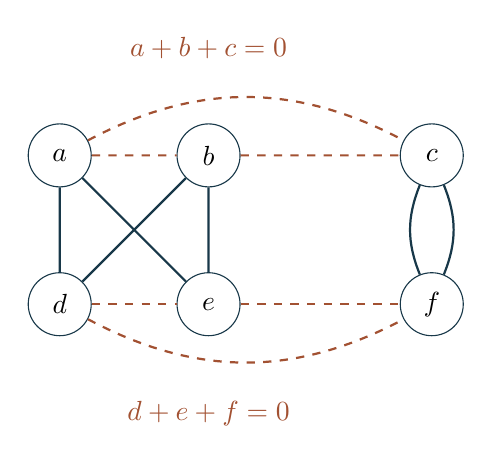
\begin{tikzpicture}[scale=1.05,
v/.style={circle,draw=ink,fill=white,minimum size=8mm,inner sep=1pt},
pair/.style={draw=ink,thick},
hyper/.style={draw=warm,dashed,thick}]
\node[v] (a) at (0,1.8) {\(a\)};
\node[v] (b) at (1.8,1.8) {\(b\)};
\node[v] (d) at (0,0) {\(d\)};
\node[v] (e) at (1.8,0) {\(e\)};
\node[v] (c) at (4.5,1.8) {\(c\)};
\node[v] (f) at (4.5,0) {\(f\)};
\draw[pair] (a)--(d) (a)--(e) (b)--(d) (b)--(e);
\draw[pair] (c) to[bend left=22] (f);
\draw[pair] (c) to[bend right=22] (f);
\draw[hyper] (a) to[bend left=28] (c);
\draw[hyper] (a)--(b)--(c);
\draw[hyper] (d) to[bend right=28] (f);
\draw[hyper] (d)--(e)--(f);
\node[above=7mm of b,text=warm] {\(a+b+c=0\)};
\node[below=7mm of e,text=warm] {\(d+e+f=0\)};
\end{tikzpicture}
\caption{The abstract table's pair graph and its two triple constraints. Solid edges give two balanced pair components; dashed connections mark triples. This diagram is not realizable by the distinct group supports asserted by the table.}
\end{figure}
\begin{proposition}[The labels force support collapse]\label{M02:prop:collapse}
The displayed table cannot be realized as a product table of three distinct left elements and six distinct right elements in any group.
\end{proposition}
\begin{proof}
Normalize the left elements to \((1,x,y)\) and the first right element \(a\) to \(1\). This preserves all product equalities: left-multiply the left factors by the inverse of their first factor and right-multiply all right factors by \(a^{-1}\).

The equations at \(r_4,r_3,r_5\), respectively, give
\[
e=y,\qquad d=y^{-1}x,\qquad b=xd=xy^{-1}x.
\]
The \(r_1\) equations are \(xb=1\) and \(yc=1\). Hence
\[
x^2y^{-1}x=1,\qquad y=x^3,\qquad
b=x^{-1},\quad c=x^{-3},\quad d=x^{-2}.
\]
Finally, \(r_8\) gives \(f=xc=x^{-2}=d\), contradicting distinctness.
\end{proof}
The group calculation supplies information absent from the matrix kernel, pair balance, and dyadic height tests. A universal presentation that contains torsion is likewise insufficient by itself: a proposed torsion-free quotient might kill that torsion. One must track the word and prove a support collapse or another contradiction in the quotient.

\section{Two exact barriers to a universal graph argument}\label{M02:sec:barriers}
\subsection{The deletion budget can fail on an injective cyclic example}
\begin{theorem}\label{M02:thm:budgetbarrier}
Let \(G=\langle g\rangle\cong\Z\), \(\alpha=1+g\), and \(B_n=\{1,g,\ldots,g^{n-1}\}\). Multiplication is injective on this support for every \(n\). Nevertheless, its deletion budget satisfies
\[
\sum_{j=1}^n\frac{\lambda_j}{2+\lambda_j}<1
\qquad(n\ge18).
\]
\end{theorem}
\begin{proof}
The convolution Gram matrix has diagonal two and adjacent entries one. Its eigenvalues are \(2+2\cos(k\pi/(n+1))\), \(1\le k\le n\), all positive. Deleting coordinate \(j\) leaves two path blocks of lengths \(j-1\) and \(n-j\). With \(L_j=\max(j-1,n-j)\),
\[
\lambda_j=2-2\cos\frac{\pi}{L_j+1}
\le\frac{\pi^2}{(L_j+1)^2}
\le\frac{4\pi^2}{(n+1)^2}.
\]
Therefore
\[
\sum_j\frac{\lambda_j}{2+\lambda_j}
\le\frac12\sum_j\lambda_j
\le\frac{2\pi^2n}{(n+1)^2}
<\frac{20n}{(n+1)^2}<1
\]
for \(n\ge18\), using \(\pi^2<10\) and \((n+1)^2>20n\).
\end{proof}
Thus universal strictness of Theorem~\ref{M02:thm:deletion}'s test is false even for a torsion-free cyclic group. The pair subsystem here has boundary pins and handles the example, so combining the tests is useful. The example does not show the combined method covers all groups.

\subsection{A genuine higher fiber cannot be replaced by positive edges}
\begin{proposition}\label{M02:prop:rankone}
Let \(v\in\C^r\) have at least three nonzero coordinates. If \(0\preceq L\preceq vv^*\) and \(L\) is a sum of positive semidefinite matrices each supported on at most two coordinates, then \(L=0\). In particular, \(vv^*\) itself has no such decomposition.
\end{proposition}
\begin{proof}
For \(z\perp v\), nonnegativity gives \(0\le z^*Lz\le z^*vv^*z=0\). Each positive summand also vanishes on every such \(z\), so its range lies in \(\operatorname{span}(v)\). Every nonzero summand must therefore be a positive multiple of \(vv^*\), which has at least three coordinates in its support. This contradicts the pair-support restriction.
\end{proof}
Consequently a single triple-fiber energy cannot be exactly replaced, or nontrivially bounded below, by a sum of positive pairwise energies on the same coordinates. This is a fiberwise assertion. Several fibers together can have larger range and admit useful edge-based lower bounds.

\subsection{Exact factor width: no fixed positive locality suffices}
Factor width is an established matrix notion \cite{B:BCPT}. We use its natural Hermitian version. The rank-one support obstruction and the existence of full-rank matrices of arbitrarily large factor width already occur in \cite[Proposition 3 and its following remark]{B:BCPT}. The application below concerns actual cyclic group-convolution matrices.
\begin{definition}
For \(H\succeq0\), let \(\FW(H)\) be the least integer \(k\) for which \(H\) is a finite sum of positive semidefinite matrices, each supported in a principal block on at most \(k\) coordinates. Equivalently, \(H\) is a sum of rank-one positive matrices whose generating vectors each have at most \(k\) nonzero coordinates.
\end{definition}
\begin{lemma}[Trace obstruction]\label{M02:lem:fwtrace}
If \(\FW(H)\le k\), then
\begin{equation}\label{M02:eq:fwtrace}
\one^*H\one\le k\,\tr H.
\end{equation}
Factor width is invariant under invertible diagonal congruence.
\end{lemma}
\begin{proof}
For a summand \(P\succeq0\) supported on \(S\), \(|S|\le k\),
\[
\one^*P\one
\le |S|\lambda_{\max}(P)
\le k\,\tr P.
\]
Sum over the decomposition. If \(D\) is invertible diagonal, \(P\mapsto D^*PD\) preserves positive semidefiniteness and its coordinate support. Applying the same observation to \(D^{-1}\) proves invariance.
\end{proof}
\begin{theorem}[Exact locality requirement for cyclic convolution]\label{M02:thm:factorwidth}
Let \(m\ge2\), \(n\ge m\), and let \(H_{m,n}\) be the Gram matrix of multiplication by
\[
\alpha_m=1+g+\cdots+g^{m-1}
\]
on \(B_n=\{1,g,\ldots,g^{n-1}\}\) in \(\Q[\Z]\). Then
\[
(H_{m,n})_{ij}=(m-|i-j|)_+,\qquad H_{m,n}\succ0,
\]
and
\begin{equation}\label{M02:eq:fwbound}
\left\lceil m-\frac{m^2-1}{3n}\right\rceil
\le\FW(H_{m,n})\le m.
\end{equation}
In particular,
\begin{equation}\label{M02:eq:fwexact}
\boxed{\quad n\ge m,\quad 3n>m^2-1
\quad\Longrightarrow\quad \FW(H_{m,n})=m.\quad}
\end{equation}
For every fixed \(k\ge1\), a choice \(m=k+1\), \(n=m^2\) yields an injective torsion-free convolution Gram matrix that has no positive decomposition supported on at most \(k\) coordinates, even after invertible diagonal congruence.
\end{theorem}
\begin{proof}
Two shifted strings of \(m\) ones overlap in \((m-|i-j|)_+\) positions, giving the formula. Multiplication by a nonzero polynomial cannot annihilate a nonzero polynomial, so the convolution matrix is injective and its Gram matrix is positive definite. Each of its row outer products uses at most \(m\) coordinates, proving the upper bound.

The trace is \(mn\), whereas
\begin{align*}
\one^*H_{m,n}\one
&=mn+2\sum_{r=1}^{m-1}(n-r)(m-r)\\
&=nm^2-\frac{m(m^2-1)}3.
\end{align*}
Lemma~\ref{M02:lem:fwtrace} implies
\[
\FW(H_{m,n})\ge
\frac{\one^*H_{m,n}\one}{\tr H_{m,n}}
=m-\frac{m^2-1}{3n}.
\]
Integrality gives \eqref{M02:eq:fwbound}. Under the strict hypothesis \(3n>m^2-1\), the last ratio exceeds \(m-1\), proving \eqref{M02:eq:fwexact}. The explicit choice in the last sentence meets both hypotheses, and diagonal invariance finishes the claim.
\end{proof}
The lower-bound mechanism also follows from \cite[Theorem 12]{B:BCPT}: for real positive semidefinite \(A\), that theorem bounds factor width below by the ceiling of the largest eigenvalue of its diagonally normalized matrix. Here the normalization is \(H_{m,n}/m\), and its Rayleigh quotient at \(\one\) gives exactly the lower estimate in \eqref{M02:eq:fwbound}. Thus the spectral lower-bound principle is prior art; the explicit convolution-family calculation is supplied here without a priority claim.

The strict threshold in \eqref{M02:eq:fwexact} matters: at equality the lower bound from this argument is only \(m-1\). No assertion of an exact threshold in the remaining parameter region is made.

The smallest illustrative case is
\[
H_{3,3}=
\begin{pmatrix}3&2&1\\2&3&2\\1&2&3\end{pmatrix},
\qquad
\det H_{3,3}=8,\qquad \FW(H_{3,3})=3.
\]
For a pair-supported positive block, the sum of its diagonal entries is at least twice the modulus of its off-diagonal entry. Therefore every factor-width-two matrix satisfies
\[
\tr H\ge2\sum_{i<j}|H_{ij}|.
\]
Here the two sides are \(9\) and \(10\). This provides an immediate pairwise obstruction.

Theorem~\ref{M02:thm:factorwidth} is a complete statement about an infinite family. It is obtained using elementary sparse-positive-factor bounds in an established framework, and its historical first appearance has not been established. It rules out a specified universal positive-local-decomposition strategy. It does not rule out graph methods with auxiliary variables, variable-size blocks, nonpositive identities, or additional group-theoretic input.

\section{A sound combined procedure and the unsolved step}
The results provide a sound certificate procedure for an explicitly known group product table and explicitly given coefficients:
\begin{enumerate}
\item Construct the exact fibers and \(M_{\alpha,B}\), retaining all common colour coefficients and group labels.
\item Extract singleton and pair rows. Use pins, gain inconsistency, or a positive forest minor to kill components.
\item Contract live components using Theorem~\ref{M02:thm:residual}; keep all higher-fiber residual coefficients exactly.
\item Apply residual forcing, exact minors, the uniform-coefficient forest criterion, or the dyadic test when their hypotheses hold.
\item Use phase-retaining forest coercivity on suitable deleted matrices, followed by the deletion budget or its block form.
\item Independently check noncommutative label relations. A surviving coefficient solution is not a group counterexample until the group, torsion-freeness, support distinctness, and the proposed product equalities have all been proved.
\end{enumerate}
Every successful certificate has a proof supplied above. A failed certificate is inconclusive. This is not asserted to be a terminating decision procedure for arbitrary group presentations: even recovering the exact product table can require a separate word-problem argument.
\begin{problem}[Universal coverage]\label{M02:prob:coverage}
Prove that every matrix \(M_{\alpha,B}\) arising from a torsion-free group and nonzero complex \(\alpha\) has full column rank, either by the displayed certificates or by an additional argument that covers their failure regions.
\end{problem}
The exact reduction identifies the same obligation as \(\rank Q=s\) for every remaining live-component residual system. That is an equivalent restatement within this framework, not an independent result. Theorem~\ref{M02:thm:budgetbarrier} prevents asserting universal strictness of the singleton budget. Theorem~\ref{M02:thm:factorwidth} prevents asserting a universal fixed-arity positive decomposition. Section~\ref{M02:sec:falsepositive} prevents identifying abstract coloured incidence feasibility with realizability in a torsion-free group.

In the rational support-three route, connected pair graphs with triple fibers are handled, but disconnected balanced pair components and triples joining three live components remain. The uniform-positive-coefficient forest theorem excludes another structural case, while leaving residual cycles and mixed-sign cases. Even a fully balanced pair-only system still requires a decisive use of the noncommutative labels. No theorem here shows that all such surviving systems collapse in a torsion-free group.

\section{Success-condition audit and verification record}
\begin{longtable}{@{}P{.09\linewidth}P{.25\linewidth}P{.59\linewidth}@{}}
\toprule
Gate & Verdict & Reason\\
\midrule\endhead
G1 & Preserved & The pre-existing named problem is Kaplansky's characteristic-zero zero-divisor conjecture.\\[4pt]
G2 & Preserved & The original fields, groups, supports, coefficients, and zero-product assertion are retained. Restricted lemmas are labelled as such.\\[4pt]
G3 & Open in checked sources & Current primary literature explicitly leaves characteristic zero open. Already-known support exclusions are not claimed as new resolutions.\\[4pt]
G4 & Not met & No unconditional proof for all torsion-free groups and all supports has been obtained.\\[4pt]
G5 & Not met for the original problem & The certificates and locality theorem are fully proved, but no new global group-ring case or universal coverage theorem follows.\\[4pt]
G6 & Not established & Gain balance, forest determinants, factor width and Rayleigh arguments have extensive prior art. Searches do not establish first priority for the specialized formulations.\\
\bottomrule
\end{longtable}
\subsection{What was checked}
The appendix program uses exact rational, integer, and symbolic complex arithmetic. It checks the abstract table's entries, rank, kernel, and residual contraction; mixed pins and complex gains; cycle determinants and a Hermitian Cauchy--Binet identity; the sharp deletion-budget family; and finite instances of the cyclic factor-width formulas.

The infinite-parameter theorems are justified by the displayed algebraic proofs, not by those finite tests. The nonrealizability of the abstract table is proved by the explicit group calculation, not by a numerical rank computation. No Lean or Coq verification, external referee approval, or exhaustive proof check of the source corpus is claimed.
\subsection{Priority and mathematical conclusion}
The most useful transfer in this restart is a precise way to combine phase-retaining graph certificates with deleted spectral data, while preserving higher-order fibers and group labels. The strongest proved limitation is the unbounded exact factor width of an explicit family of injective cyclic convolution matrices. These findings sharpen the research method but do not resolve the historical target.

\noindent\fcolorbox{accent}{accent!5}{\parbox{0.945\linewidth}{
\textbf{Final conclusion.} This manuscript contains complete auxiliary proofs and exact diagnostics from a fresh graph-corpus attack. It must not be cited as a proof, disproof, or claimed resolution of Kaplansky's characteristic-zero zero-divisor conjecture.
}}


\section{Self-contained exact-check program}
The program below requires Python 3 and SymPy. Copy the listing to a file and run it. Its final status explicitly distinguishes finite successful checks from a global proof. Graph and matrix data are embedded; no input data file is required.
\begin{lstlisting}
"""Exact checks for the graph-based Kaplansky research note.

Python 3 and SymPy are required. These checks do not prove Kaplansky.
"""
from collections import defaultdict
from itertools import combinations
import json
import sympy as s


def contract_pairs(M):
    """Return T,R with ker(M) = T ker(R), using exact arithmetic."""
    n = M.cols
    adj = [[] for _ in range(n)]
    pins, higher = set(), []
    for i in range(M.rows):
        nz = [j for j in range(n) if M[i, j] != 0]
        if len(nz) == 1:
            pins.add(nz[0])
        elif len(nz) == 2:
            u, v = nz
            gain = s.cancel(-M[i, u] / M[i, v])
            adj[u].append((v, gain))
            adj[v].append((u, 1 / gain))
        elif len(nz) > 2:
            higher.append(i)
    seen, live = set(), []
    for root in range(n):
        if root in seen:
            continue
        transport = {root: s.Integer(1)}
        todo, bad = [root], False
        seen.add(root)
        while todo:
            u = todo.pop()
            bad = bad or u in pins
            for v, gain in adj[u]:
                wanted = s.cancel(transport[u] * gain)
                if v in transport:
                    bad = bad or s.simplify(transport[v]-wanted) != 0
                else:
                    transport[v] = wanted
                    seen.add(v)
                    todo.append(v)
        if not bad:
            live.append(transport)
    T = s.zeros(n, len(live))
    for c, transport in enumerate(live):
        for j, value in transport.items():
            T[j, c] = value
    R = M.extract(higher, list(range(n))) * T
    assert M.rank() == n - T.cols + R.rank()
    return T, R


# Abstract colour table: deliberately NOT a group product table.
table = [[1,5,7,2,4,8], [3,1,8,5,6,2], [4,6,1,3,2,7]]
assert all(len(set(row)) == 6 for row in table)
assert all(len({table[i][j] for i in range(3)}) == 3
           for j in range(6))
M = s.zeros(8, 6)
for i in range(3):
    for j in range(6):
        M[table[i][j]-1, j] += 1
z = s.Matrix([1,1,-2,-1,-1,2])
assert M*z == s.zeros(8,1) and M.rank() == 5
assert [sum(M[i,j] for i in range(8)) for j in range(6)] == [3]*6
assert [sum(M[i,j] for j in range(6)) for i in range(8)] == [3,3,2,2,2,2,2,2]
T, R = contract_pairs(M)
assert T.cols == 2 and R.rank() == 1

# Mixed singleton, pair and higher rows: pins and complex gains.
examples = [
    s.Matrix([[1,-1,0],[0,1,-1],[1,1,1]]),
    s.Matrix([[1,1,0],[0,1,1],[1,0,1]]),
    s.Matrix([[1,0,0,0],[1,s.I,0,0],[0,1,1,1]]),
    s.Matrix([[1,2,0],[0,1,3],[2,4,0],[1,1,1]])]
for A in examples:
    contract_pairs(A)

# Exact cycle determinant and Cauchy--Binet with actual Hermitian adjoint.
p1,p2,p3,q1,q2,q3 = s.symbols('p1 p2 p3 q1 q2 q3')
C = s.Matrix([[p1,q1,0],[0,p2,q2],[q3,0,p3]])
assert s.expand(C.det()-p1*p2*p3-q1*q2*q3) == 0
N = s.Matrix([[2,-1,0],[0,1,-s.I],[1,0,1],[1,0,0]])
minor_sum = sum(s.expand_complex(abs(N[list(S),:].det())**2)
                for S in combinations(range(N.rows), N.cols))
assert s.simplify((N.conjugate().T*N).det()-minor_sum) == 0

# Sharp deletion budgets: exact rational spectra are known analytically.
for n in range(3,12):
    for eps in [s.Integer(0), s.Rational(1,7)]:
        a, b = s.Rational(n,n-1)+eps, -s.Rational(1,n-1)
        d, lam, deleted = a+b, a+n*b, a+(n-1)*b
        assert s.simplify(n*(deleted-lam)/(d+deleted-2*lam)) == 1
        if eps == 0:
            assert n*deleted/(d+deleted) == 1
        else:
            assert n*deleted/(d+deleted) > 1

# The universal deletion strictness fails: exact rational upper bound.
for n in range(18,101):
    assert s.Rational(20*n,(n+1)**2) < 1

# True cyclic-group convolution and the factor-width obstruction.
def cyclic_gram(m,n):
    C = s.zeros(m+n-1,n)
    for j in range(n):
        for i in range(m):
            C[i+j,j] = 1
    return C.T*C

H3 = cyclic_gram(3,3)
assert H3 == s.Matrix([[3,2,1],[2,3,2],[1,2,3]])
assert H3.det() == 8 and s.trace(H3) == 9
assert 2*sum(abs(H3[i,j]) for i in range(3) for j in range(i+1,3)) == 10
for m in range(2,11):
    n = max(m, (m*m-1)//3+1)
    H = cyclic_gram(m,n)
    total = sum(H)
    assert total == n*m*m-s.Rational(m*(m*m-1),3)
    assert s.trace(H) == n*m
    assert s.Rational(total,n*m) > m-1
    assert all(H[:k,:k].det() > 0 for k in range(1,min(n,4)+1))

# Dyadic gain consistency: orientations matter beyond bipartiteness.
assert 2*2*s.Rational(1,2)*s.Rational(1,2) == 1
assert 2**4 != 1
assert (-2)*2*s.Rational(1,2)*s.Rational(1,2) == -1

print(json.dumps({
    'status':'all exact assertions passed',
    'abstract_table_rank':int(M.rank()),
    'pair_components':int(T.cols),
    'residual_rank':int(R.rank()),
    'group_nonrealizability_proof':'in manuscript, not checked by this program',
    'cyclic_3_by_3_gram_determinant':int(H3.det()),
    'global_Kaplansky_conjecture_proved':False,
    'formal_proof_assistant_verification':False
},indent=2))
\end{lstlisting}

\section{Source ledger}
The following corpus identifiers refer to the pinned snapshot in Section 2:
\begin{itemize}
\item [016] \emph{Universal Weighted-Laplacian Cones and the Maximal-Cusp Spectral Link}: the subsection on spanning forests, Lemma \emph{Rooted-forest coefficients}.
\item [160] \emph{Wagner Forest SOS Obstruction}: forced norms and cycle dependence on the prescribed supports.
\item [194] \emph{Compensated Pair Kernels and Exact Defect Decompositions for the Zhang--Wu Line-Graph Randi\'c Conjecture}: local pair identities and antisymmetric transfer.
\item [212] \emph{Randi\'c Extremal Matchings}: fractional matching split and the stated Randi\'c lower bound.
\item [226] \emph{Fajtlowicz Average Distance Proof}: stationarity--deletion principle.
\item [227] \emph{Fajtlowicz Proof Audit}: the normalized probability constraint and deletion accounting.
\end{itemize}
These are inspected research drafts. Their mechanisms motivate independently proved statements in this manuscript. Their broader claimed conclusions are not used as unverified premises.



\chapter{Projective Arithmetic and Moment Methods}\label{chap:M03}
\noindent{\small\color{quiet}\textbf{Source manuscript M03.} 22 November 2026.}\par
\compilationnote{The projective and arithmetic assertions concern actual coefficients.
Their coefficient and group hypotheses remain in force. Algebraicity is
not rationality, and a degree bound is not emptiness of the coefficient
locus. Augmentation and jet refinements appear in Chapter~\ref{chap:M13}.}
\subsection*{Original abstract}
We restart the characteristic-zero zero-divisor problem using a broader set of methods from the Verifiable Mathematical Reasoning Corpus. The main route treats zero-product coefficients as a projective incidence variety. For a torsion-free group, projective boundary intersection proves that a zero divisor with support size \(m\) has projective coefficient transcendence degree at most \(m-3\). A pair of minimum total support \(m+n\), if one exists, has a joint normalized coefficient field of degree at most \(\binom{m+n-2}{m-1}\).

For support three, the actual coefficient ratios are consequently algebraic. Reduction at finite places makes them algebraic units, while Hilbert-space equality analysis imposes strict triangle inequalities at every embedding. These restrictions yield a finite coefficient catalogue over every quadratic number field. Combined with finite \(p\)-group augmentation, they exclude all support-at-most-three zero divisors over quadratic fields other than \(\Q(\sqrt{-3})\) for torsion-free residually finite \(p\)-groups, provided \(p\ne3\) and \((L,p)\ne(\Q(\sqrt5),5)\). No bound on an annihilator's support or on coefficient height occurs in this statement.

A second route uses the full convolution operator. Exact Christoffel moment bounds give support exclusions, an all-orders free-model formula, and a sharp obstruction: positive integral algebraic moments and an integral formal determinant can still carry a nonzero atom at zero. The manuscript supplies proofs, exact checks, corpus provenance, and a prior-work audit. It does not solve the original global conjecture and does not establish historical priority for the specialized results.
\medskip
\section{The unchanged problem and the new starting point}
The target is the characteristic-zero form of Kaplansky's historical Problem~6, associated with the 1956 conference and published in its 1957 report \cite{B:Kaplansky}:
\begin{equation}\label{M03:eq:target}
\boxed{\KZ:\quad
\begin{gathered}
G\text{ torsion-free},\quad \operatorname{char}K=0,\quad
\alpha,\beta\in K[G],\\
\alpha\beta=0\quad\Longrightarrow\quad \alpha=0\text{ or }\beta=0.
\end{gathered}}
\end{equation}
All supports are finite by the definition of a group algebra. There is no bound on their sizes, and no residual-finiteness, ordering, amenability, or coefficient-degree assumption in \eqref{M03:eq:target}. Recent primary literature still distinguishes the open characteristic-zero question from positive-characteristic constructions \cite{B:Ivanov}. The latter are not substituted for the former.

The preceding investigations studied exact collision certificates and finite graph reductions. This restart puts the \emph{coefficient variety} and the \emph{full regular convolution operator} first. Its principal questions are:
\begin{enumerate}
\item Can a positive-dimensional family of zero-product coefficients be specialized to a smaller support?
\item What arithmetic restrictions remain when no such support decrease is possible?
\item Can a full-operator moment sequence exclude finite-support annihilators without a spectral gap?
\end{enumerate}
The first two questions lead to the projective and quadratic-field results below. The third yields a valid independent certificate but also a precise limitation.

\paragraph{Terminology.}
In this paper, an element is \emph{right regular} if it has no nonzero right annihilator. All statements about a three-term element concern this sense. Applying the involution or using the opposite group gives the corresponding left statement. A group is \emph{residually a finite \(p\)-group} if every nonidentity element survives in some finite \(p\)-group quotient. Taking the product of finitely many such quotients separates any prescribed finite set.

\paragraph{What has actually expanded.}
The quadratic coefficient catalogue and the residual-\(p\) application give explicit, fully quantified partial exclusions absent from the two earlier manuscripts. They are not merely tests up to a finite support bound. They still leave the rational support-three problem for arbitrary torsion-free groups, larger supports, and arbitrary algebraic coefficient degree. No claim that a new \emph{group class with unrestricted supports} has been solved is made.

\section{Corpus synthesis and the hypotheses retained}
The source snapshot is
\begin{center}\small\texttt{884d261108a87d2229e5bcc273e5f4a607c771d2}.\end{center}
The repository contained 487 tracked files, including 227 TEX files. Its available remote head was rechecked for this restart. The whole TEX title inventory was scanned; selected proof passages were read in detail. This is not a claim that all 227 manuscripts were independently verified.

\begin{longtable}{@{}P{22mm}P{49mm}P{80mm}@{}}
\toprule Corpus & Actual method inspected & Transfer made, or missing hypothesis\\
\midrule\endhead
[069], [070] & Excluding a projective boundary; generic sections; B\'ezout degree & Replace the spectral scheme by a zero-product incidence scheme. Support minimality, not a spectral identity, excludes its boundary.\\[5pt]
[061] & Level-set degeneration & Motivates support specialization. Its all-parameter Floquet identity is not assumed for group rings.\\[5pt]
[013], [045] & Primitive local normalization; finite-dimensional descent & Normalize at one valuation at a time; keep a fixed finite multiplication matrix when descending fields.\\[5pt]
[010], [089], [060] & Trace/norm constraints; least-valuation arguments; fixed multiplicative data & Combine unit ratios with inequalities at every embedding. Density zero is not substituted for emptiness.\\[5pt]
[001], [019], [026] & Actual positive measures; inverse Gram expressions; Hankel determinants & Construct the regular spectral measure and derive exact constrained moment minima.\\[5pt]
[037], [099] & Return-count recurrences; moment rigidity & Prove the free-model recurrence directly. Arbitrary group moments are not presumed D-finite or atom-free.\\[5pt]
[078], [088], [112], [178] & Frobenius, arithmetic power series, natural-boundary arguments & Ordinary noncommutative Frobenius fails. A cyclic trace identity survives, but does not force zero spectral mass.\\[5pt]
[085] & Well-founded decoder trees & The actual decoder identities have only trivial images in groups; their nonassociative models cannot be imported.\\[5pt]
[095], [193] & Cancellation profiles; composition with exact cross terms & No factorial-tail or universal positive-gluing hypothesis is available here. Common vocabulary does not supply a transfer.\\
\bottomrule
\end{longtable}
The projective mechanism in [069] is explicitly attributed there to existing spectral work. The geometry, valuation arguments, and Christoffel theory used here are established tools. The question is what their correctly proved group-ring specializations say; historical novelty is a separate issue.

\section{Projective support descent}\label{M03:sec:projective}
Fix distinct elements
\[
A=\{a_1,\ldots,a_m\},\qquad B=\{b_1,\ldots,b_n\}
\]
of a group. For variables \(X=(X_1,\ldots,X_m)\), let \(M(X)\) be the matrix with rows indexed by \(AB\), columns by \(B\), and entries
\[
M(X)_{g,j}=\begin{cases}X_i,&a_i b_j=g,\\0,&\text{otherwise}.\end{cases}
\]
Group cancellation makes the index \(i\) unique. Thus
\begin{equation}\label{M03:eq:exactmatrix}
M(x)y=0\quad\Longleftrightarrow\quad
\left(\sum_i x_i a_i\right)\left(\sum_jy_jb_j\right)=0.
\end{equation}
Define the projective rank-deficient locus
\begin{equation}\label{M03:eq:Z}
Z_{A,B}=\{[x]\in\PP^{m-1}_{\C}:\rank M(x)<n\}.
\end{equation}
It is cut out over \(\Q\) by homogeneous \(n\)-minors of degree \(n\). There are at least \(n\) rows, since \(a_1B\subset AB\). Each coordinate point is absent from \(Z_{A,B}\), because multiplication by a single group element is injective.

\begin{lemma}[Field descent with the left factor fixed]\label{M03:lem:descent}
Let \(L\subset E\) be fields, \(G\) a group, and \(\alpha\in L[G]\). A nonzero finite-support annihilator of \(\alpha\) in \(E[G]\) implies one in \(L[G]\), supported inside the original right support.
\end{lemma}
\begin{proof}
Use the finite matrix \(M(x)\) on that support. Its rank is unchanged by field extension because rank is characterized by nonzero minors. A nonzero kernel over \(E\) therefore implies a nonzero kernel over \(L\). Some right coefficients may vanish after descent; this is harmless.
\end{proof}

\begin{lemma}[One and two terms]\label{M03:lem:two}
Over any field, a nonzero element of support at most two in the group algebra of a torsion-free group is right regular.
\end{lemma}
\begin{proof}
A one-term element is a unit. After multiplying a two-term element by a unit on the left, it has the form \(1-cg\), with \(c\ne0\) and \(g\ne1\). If \(\beta=cg\beta\ne0\), its finite nonempty support is invariant under translation by \(g\). A permutation of a finite set has finite order, giving \(g^k b=b\) for some \(b\) and \(k>0\). Hence \(g^k=1\), a contradiction.
\end{proof}

We use the elementary projective intersection theorem: nonempty projective closed sets in \(\PP^N\) of dimensions \(r,s\) meet whenever \(r+s\ge N\); their intersection then has dimension at least \(r+s-N\) \cite[Lemma 33.34.3]{B:StacksProjective}. In particular a positive-dimensional projective variety meets every hyperplane.

\begin{theorem}[Support--transcendence descent]\label{M03:thm:trdeg}
Suppose \(G\) is torsion-free and
\[
0\ne\alpha=\sum_{i=1}^m x_i a_i\in\C[G],\qquad
\alpha\beta=0\ne\beta,
\]
where all \(x_i\ne0\). Put
\[
t=\trdeg_{\Q}\Q(x_2/x_1,\ldots,x_m/x_1).
\]
For any choice of \(t\) coordinates, there exists a nonzero zero-divisor left factor supported on the remaining at most \(m-t\) elements of \(A\), with a nonzero annihilator supported inside \(\supp\beta\). Consequently
\begin{equation}\label{M03:eq:trdeg}
\boxed{t\le m-3.}
\end{equation}
In particular, every support-three zero divisor has \emph{actual} projective coefficient ratios in \(\Qbar\).
\end{theorem}
\begin{proof}
The \(\Q\)-Zariski closure of \([x]\) is a projective subvariety of dimension \(t\). All defining minors of \(Z_{A,B}\) vanish at \([x]\) and have rational coefficients, so this closure lies in \(Z_{A,B}\). After base change to \(\C\), choose a component of dimension \(t\). The coordinate linear space obtained by setting any chosen \(t\) coordinates to zero has dimension \(m-1-t\). The projective intersection theorem gives an intersection point. At that point \(M\) has a nonzero kernel, proving the support decrease.

If \(t\ge m-2\), one may instead intersect with \(m-2\) coordinate hyperplanes, leaving at most two left support elements. Lemma~\ref{M03:lem:two} rules this out. Hence \eqref{M03:eq:trdeg}. For \(m=3\), transcendence degree zero of this finitely generated field means it is a number field.
\end{proof}

\begin{corollary}[An all-group coefficient exclusion]\label{M03:cor:transcoeff}
For every torsion-free group, every \(m\)-term element whose projective coefficient field has transcendence degree at least \(m-2\) is right regular. In particular, a three-term element with even one transcendental coefficient ratio is right regular, with no restriction on the possible annihilator support.
\end{corollary}
This is stronger than merely replacing a hypothetical counterexample by a different algebraic-coefficient example. It controls the coefficients of the given element. It does not exclude algebraic ratios.

\begin{theorem}[Finite coefficient locus at minimum left support]\label{M03:thm:mindegree}
Suppose \(m\) is the minimum left support size of a nonzero zero divisor in \(\C[G]\). For fixed \(A,B\) of sizes \(m,n\), the locus \(Z_{A,B}\) is finite, and every point in it satisfies
\begin{equation}\label{M03:eq:detdegree}
[\Q(x_2/x_1,\ldots,x_m/x_1):\Q]\le n^{m-1}.
\end{equation}
If \(G\) is torsion-free and \(m=3\), this conclusion applies whenever a support-three zero divisor exists, without an additional minimality assumption.
\end{theorem}
\begin{proof}
No point of \(Z_{A,B}\) can have a zero coordinate: it would give a nonzero zero divisor with smaller left support. A positive-dimensional projective component would meet a coordinate hyperplane. Thus \(Z_{A,B}\) is finite.

Let \(r=m-1\). Select \(r\) general rational linear combinations of the degree-\(n\) minors. They cut \(\PP^r\) to a zero-dimensional scheme containing \(Z_{A,B}\): at each step the finite base locus prevents any positive-dimensional component from being contained in every available equation, and a general combination avoids the finitely many bad choices. Projective B\'ezout bounds the length of this complete intersection by \(n^r\). Hence there are at most \(n^r\) geometric points in \(Z_{A,B}\). Every point is algebraic, and its distinct Galois conjugates, whose number is the degree in \eqref{M03:eq:detdegree}, are among those points. Characteristic zero ensures separability.

The last statement follows from Lemma~\ref{M03:lem:two}.
\end{proof}

\subsection{A sharper bound for a minimum-total-support pair}
The bilinear incidence variety gives a sharper joint field bound.

\begin{theorem}[Segre bound for a smallest pair]\label{M03:thm:segre}
Suppose \(\C[G]\) has nonzero zero divisors, and choose a pair \(\alpha\beta=0\) with \(m+n=|\supp\alpha|+|\supp\beta|\) minimum. Write its nonzero coefficients as \(x_i,y_j\). Then their joint normalized field
\[
L=\Q(x_2/x_1,\ldots,x_m/x_1,y_2/y_1,\ldots,y_n/y_1)
\]
is a number field and
\begin{equation}\label{M03:eq:segre}
\boxed{[L:\Q]\le\binom{m+n-2}{m-1}.}
\end{equation}
\end{theorem}
\begin{proof}
Inside \(\PP^{m-1}\times\PP^{n-1}\), impose every exact product equation
\[
f_g(X,Y)=\sum_{a_i b_j=g}X_iY_j=0.
\]
Call the resulting projective scheme \(W\). A point with any zero coordinate in either factor would give a nonzero zero-product pair with smaller total support. Thus its underlying closed set lies entirely in the product of the two coordinate tori. This is an affine open subset of the projective product. A projective closed set contained in an affine variety is finite; equivalently, in the Segre embedding any positive-dimensional component must meet the hyperplane \(X_1Y_1=0\), which is excluded here.

The Segre variety \(S\) has dimension \(d=m+n-2\). Each \(f_g\) is a linear equation in its Segre coordinates. Because their common base locus \(W\) is finite, choose \(d\) general rational linear combinations cutting \(S\) properly at each step. The resulting finite linear section contains \(W\). Its length is \(\deg S\), so the number of geometric points of \(W\), and hence the Galois orbit of our point, is at most \(\deg S\).

For completeness, the degree follows from the graded Hilbert function of the Segre embedding:
\[
\dim H^0(S,\OO_S(k,k))
=\binom{k+m-1}{m-1}\binom{k+n-1}{n-1}.
\]
Its leading coefficient is \(1/((m-1)!(n-1)!)\). Multiplying by \(d!\) gives \(\deg S=\binom{m+n-2}{m-1}\). The normalized coordinates recover the point from its Segre coordinates, so the Galois orbit size is exactly \([L:\Q]\).
\end{proof}

\begin{remark}[What the degree bound does not give]
The total support \(m+n\) is unbounded. A finite coefficient locus can be nonempty, and \eqref{M03:eq:segre} does not bound coefficient height. These theorems cannot turn an infinite search into a proof merely by replacing complex numbers with finitely many algebraic possibilities at a fixed size.
\end{remark}

\paragraph{A sharp calibration outside the target.}
In the finite cyclic group \(C_q=\langle g\rangle\), take \(A=\{1,g\}\) and \(B=C_q\). The matrix of multiplication by \(x+yg\) has determinant
\[
x^q-(-y)^q.
\]
It gives exactly \(q\) projective coefficient points, each with a one-dimensional full-support kernel. The corresponding bilinear incidence consists of \(q=\binom{q}{1}\) points. Thus the Segre point count can be sharp for group-product matrices. This example has torsion and is not a counterexample to \eqref{M03:eq:target}.

\section{Arithmetic rigidity of three coefficients}\label{M03:sec:arithmetic}
The preceding section makes the arithmetic route applicable to the \emph{actual} coefficients of every support-three complex zero divisor.

\begin{theorem}[Unit ratios at every finite place]\label{M03:thm:units}
Let \(G\) be torsion-free and let
\(\alpha=c_1a_1+c_2a_2+c_3a_3\in L[G]\), where \(L\) is a number field, the \(a_i\) are distinct, and all coefficients are nonzero. If \(\alpha\) has a nonzero finite-support annihilator over an extension of \(L\), then
\begin{equation}\label{M03:eq:units}
c_i/c_j\in\OO_L^\times\qquad(1\le i,j\le3).
\end{equation}
\end{theorem}
\begin{proof}
By Lemma~\ref{M03:lem:descent}, choose an annihilator in \(L[G]\). Fix a nonzero prime ideal \(\mathfrak p\) and its normalized valuation. Independently rescale the two factors so that each minimum coefficient valuation is zero. The factors are integral at \(\mathfrak p\), their reductions are nonzero, and their product remains zero.

If the three valuations in the left factor were not all equal, only one or two coefficients would survive its reduction. This contradicts Lemma~\ref{M03:lem:two} over the residue field. Hence the three valuations agree at every finite prime. Each ratio consequently has valuation zero at every finite prime, which is exactly \eqref{M03:eq:units}.
\end{proof}
This extends the familiar rational modular reduction in Abdollahi--Taheri \cite[Theorem 1.1 and its proof]{B:ATrational}; over \(\Q\), the unit ratios are just \(\pm1\). For support greater than three, the same proof says only that at least three coefficients attain the minimum valuation. It does not force all coefficient ratios to be units.

\begin{lemma}[The equality boundary of dominance]\label{M03:lem:dominance}
Let \(G\) be torsion-free and \(\alpha=\sum_{i=1}^m c_i g_i\in\C[G]\), with distinct support elements and \(m\ge2\). If
\begin{equation}\label{M03:eq:dominance}
|c_k|\ge\sum_{i\ne k}|c_i|
\end{equation}
for some \(k\), then \(\alpha\) is right regular.
\end{lemma}
\begin{proof}
If \(\alpha\beta=0\ne\beta\), regard \(\beta\) as a vector in \(\ell^2(G)\). Translation is unitary, so
\[
|c_k|\|\beta\|_2
=\left\|\sum_{i\ne k}c_i g_i\beta\right\|_2
\le\sum_{i\ne k}|c_i|\|\beta\|_2.
\]
Strict inequality in \eqref{M03:eq:dominance} is impossible. At equality, equality in the Hilbert-space triangle inequality forces all the nonzero summands to be positive multiples of a common vector. They are also scalar multiples of \(g_k\beta\). Thus \(g_k^{-1}g_i\beta\) is a scalar multiple of \(\beta\) for some \(i\ne k\). Its finite nonempty support is invariant under a nonidentity translation, contradicting torsion-freeness as in Lemma~\ref{M03:lem:two}. For \(m=2\), that scalar-multiple relation follows directly from the two-term equation.
\end{proof}

\begin{corollary}[All conjugate triangles]\label{M03:cor:triangle}
Under the hypotheses of Theorem~\ref{M03:thm:units}, every embedding \(\sigma:L\hookrightarrow\C\) satisfies
\[
|\sigma(c_i)|<|\sigma(c_j)|+|\sigma(c_k)|
\quad(\{i,j,k\}=\{1,2,3\}).
\]
\end{corollary}
\begin{proof}
Apply \(\sigma\) to the descended zero product and use Lemma~\ref{M03:lem:dominance}. Nonzero coefficients remain nonzero.
\end{proof}

\subsection{A finite catalogue over all quadratic fields}
Let \(\mu_r\) denote the \(r\)-th roots of unity and put \(\ph=(1+\sqrt5)/2\).

\begin{theorem}[Quadratic coefficient catalogue]\label{M03:thm:quadratic}
Let \([L:\Q]\le2\), \(G\) be any torsion-free group, and \(\alpha\) a support-three element with projective coefficient field contained in \(L\). If \(\alpha\) has a nonzero finite-support annihilator, its coefficient tuple, up to a common nonzero scalar and permutation, is in this list:
\begin{center}
\begin{tabular}{@{}P{57mm}P{87mm}@{}}
\toprule Field & Necessary normalized coefficients\\
\midrule
\(L\notin\{\Q(i),\Q(\sqrt{-3}),\Q(\sqrt5)\}\) & Three signs in \(\{1,-1\}\).\\[4pt]
\(L=\Q(i)\) & Three elements of \(\mu_4\).\\[4pt]
\(L=\Q(\sqrt{-3})\) & Three elements of \(\mu_6\).\\[4pt]
\(L=\Q(\sqrt5)\) & Independent signed versions of \((1,1,1)\), \((1,1,\ph)\), or \((1,\ph,\ph)\).\\
\bottomrule
\end{tabular}
\end{center}
Every coefficient tuple outside the list is right regular for every torsion-free group. No bound on coefficient height or annihilator support is required.
\end{theorem}
\begin{proof}
By Theorem~\ref{M03:thm:units}, all normalized coefficients are algebraic units.

In an imaginary quadratic field, a unit has norm one and absolute value one. Its integral trace lies in \([-2,2]\). The resulting quadratic polynomials give only \(\pm1\), the fourth roots of unity in \(\Q(i)\), or the third and sixth roots in \(\Q(\sqrt{-3})\). This proves the imaginary cases.

In a real quadratic field, order the absolute values at one embedding and divide by the coefficient of smallest absolute value. Write the magnitudes as
\[
(1,u,v),\qquad 1\le u\le v.
\]
The numbers \(u,v\) are positive units. Their conjugate magnitudes are \((1,1/u,1/v)\), since each unit norm has absolute value one. Corollary~\ref{M03:cor:triangle} yields
\[
v<1+u,\qquad 1<1/u+1/v.
\]
Consequently
\begin{equation}\label{M03:eq:smallunits}
1\le v/u<2,\qquad 1\le u<2.
\end{equation}
There is exactly one positive real quadratic unit in \((1,2)\): \(\ph\). Indeed, a unit \(\epsilon\) in that interval has norm \(\pm1\) and integral trace \(\epsilon+N(\epsilon)/\epsilon\). For norm \(+1\), the trace is strictly between \(2\) and \(5/2\), containing no integer. For norm \(-1\), it is strictly between \(0\) and \(3/2\), so it must be \(1\). This gives \(\epsilon^2-\epsilon-1=0\).

Thus \(u\) and \(v/u\) each lie in \(\{1,\ph\}\). If both equal \(\ph\), then \(v=\ph^2=1+\ph\), contradicting the strict triangle inequality. The other three possibilities are exactly the listed patterns. If \(L\ne\Q(\sqrt5)\), only \((1,1,1)\) remains. Over \(\Q\), the unit assertion directly gives signs.
\end{proof}

\paragraph{Scope of the catalogue.}
The entries in the list are surviving \emph{necessary} forms. They are not examples of zero divisors. In particular \((1,1,1)\) survives all local tests and retains a central unresolved part of the original problem. The projective theorem does not bound the coefficient-field degree by two; Theorem~\ref{M03:thm:quadratic} treats only that degree range.

\paragraph{Examples with unrestricted right support.}
For distinct \(a,b,c\) in any torsion-free group, each of
\[
a+\sqrt2\,b+\sqrt3\,c,\qquad
a+(1+\sqrt2)b+(1+\sqrt2)c,\qquad
a+\ph b+\ph^2c
\]
is right regular over \(\C\). The first follows from a nonunit coefficient ratio in its number field. The second has a dominant coefficient at the other real embedding. The third uses the \emph{equality} case \(\ph^2=1+\ph\). These are illustrations of the proved criteria, not newly named problems.

\section{An application to residually finite \texorpdfstring{\(p\)}{p}-groups}\label{M03:sec:residualp}
The catalogue can be connected to a group-theoretic input that actually excludes whole coefficient families.

\begin{lemma}[Augmentation at one good place]\label{M03:lem:augmentation}
Let \(G\) be residually a finite \(p\)-group, \(L\) a number field, and \(\alpha\in\OO_L[G]\). If its augmentation \(s=\sum_g\alpha_g\) is a unit at one prime \(\mathfrak p\) above \(p\), then \(\alpha\) is right regular over \(L\), and over every extension of \(L\).
\end{lemma}
\begin{proof}
An annihilator may first be descended to \(L\), then rescaled to be \(\mathfrak p\)-integral with nonzero reduction. Choose a finite \(p\)-group quotient injective on that reduced support. The image of the annihilator is nonzero, whereas the image of \(\alpha\) has nonzero augmentation and is invertible in the residue-field group algebra.

Here is a proof of the latter fact. The augmentation ideal of a finite \(p\)-group in characteristic \(p\) is nilpotent. Induct on the group order, using a central subgroup \(\langle z\rangle\) of order \(p\). Modulo \(z-1\), the augmentation ideal is nilpotent by induction. A sufficiently high power of the original ideal is therefore contained in \((z-1)\); its \(p\)-th power is zero because \((z-1)^p=z^p-1=0\) and \(z-1\) is central. An element of nonzero augmentation is a nonzero scalar times \(1+u\) with \(u\) nilpotent, and has a finite geometric-series inverse. This contradicts the reduced zero product.
\end{proof}
The rational version is the mechanism of \cite[Proposition 2.1 and Theorem 1.2]{B:ATrational}. The point here is to retain all residue places of the quadratic field rather than only a rational coefficient sum.

\begin{theorem}[Quadratic support-three exclusion]\label{M03:thm:residualp}
Let \(G\) be torsion-free and residually a finite \(p\)-group, and let \([L:\Q]\le2\). Suppose
\begin{equation}\label{M03:eq:exceptions}
L\ne\Q(\sqrt{-3}),\qquad p\ne3,\qquad
(L,p)\ne(\Q(\sqrt5),5).
\end{equation}
Then every nonzero element of support at most three in \(L[G]\) is right regular, including against annihilators over any extension field of \(L\).
\end{theorem}
\begin{proof}
The one- and two-term cases are Lemma~\ref{M03:lem:two}. If a three-term counterexample existed, normalize its coefficients using Theorem~\ref{M03:thm:quadratic}.

For the sign catalogue, the augmentation is \(\pm1\) or \(\pm3\), a unit at every prime above \(p\ne3\).

For \(L=\Q(i)\), divide by the first root of unity. The augmentation is \(1+u+v\) with \(u,v\in\mu_4\). The possible values are
\[
\pm1,\quad\pm i,\quad1\pm2i,\quad2\pm i,\quad3,
\]
of norms \(1,5,9\). If \(p\notin\{3,5\}\), every such value is a unit above \(p\). For \(p=5\), a value of norm \(5\) is divisible by only one of the two distinct prime ideals above \(5\), so it is a unit at the other. Thus a good place exists for every \(p\ne3\).

For \(L=\Q(\sqrt5)\), the sign pattern has already been treated. The signed sums from \((1,1,\ph)\) and \((1,\ph,\ph)\) are nonzero and have norms in \(\{-5,-1,1,5\}\). This is obtained directly from \(\ph+\ph'=1\) and \(\ph\ph'=-1\). All are units above \(p\ne5\). Lemma~\ref{M03:lem:augmentation} now contradicts every case allowed by \eqref{M03:eq:exceptions}.
\end{proof}

\begin{corollary}[Two residual primes]\label{M03:cor:twoprimes}
If \(G\) is torsion-free and is residually a finite \(p\)-group and residually a finite \(q\)-group for two distinct primes, then every nonzero element of support at most three over every quadratic number field \(L\ne\Q(\sqrt{-3})\) is right regular.
\end{corollary}
\begin{proof}
Use the catalogue for the individual hypothetical element. Sign and Gaussian patterns have only the possible bad prime \(3\). Genuine golden patterns have only the possible bad prime \(5\); the rational sign patterns within \(\Q(\sqrt5)\) still have only \(3\). Of two distinct residual primes, at least one is good for that particular pattern. Lemma~\ref{M03:lem:augmentation} applies.
\end{proof}

\paragraph{Why the exceptions have not been removed.}
In \(\Q(\sqrt5)\), the augmentation \(2+\ph\) has norm \(5\), and \(5\) ramifies. The Gaussian argument using the other prime does not apply. In the Eisenstein field, \(1+\omega+\omega^2=0\) gives an entire allowed coefficient pattern with zero augmentation. Neither observation constructs a zero divisor; it shows exactly why the present augmentation proof stops.

\paragraph{Relation to the full conjecture.}
Theorem~\ref{M03:thm:residualp} quantifies over every annihilator support and every torsion-free residually finite \(p\)-group satisfying the stated conditions. It is therefore a complete theorem on its stated range. It does not remove the restriction to three left support elements, to residual \(p\)-finiteness, or to quadratic coefficients. The rational subcase was already established in \cite{B:ATrational}. No priority or non-subsumption claim is made for the quadratic extension.

\subsection{A rational reduction for the surviving golden forms}
Up to common scaling, permutation, and Galois conjugation, every genuinely golden pattern can be written
\[
\alpha=P+\ph,\qquad P=\pm g\pm h,
\]
after a group translation, with distinct nonidentity \(g,h\). For \((1,\ph,\ph)\), divide by \(\ph\) and conjugate, using \((\ph^{-1})'=-\ph\). If \((P+\ph)\beta=0\), then
\begin{equation}\label{M03:eq:goldnorm}
(P+\ph')(P+\ph)\beta=(P^2+P-1)\beta=0.
\end{equation}
The factors commute because both are polynomials in the same \(P\) with central scalars. The rational element \(P^2+P-1\) has support at most seven and is nonzero: its augmentation is \(t^2+t-1\) for \(t\in\{-2,0,2\}\), hence \(1,-1,\) or \(5\). Lemma~\ref{M03:lem:descent} produces a rational annihilator. Equation~\eqref{M03:eq:goldnorm} is an exact reduction, not a proof that every resulting rational element is regular.

\section{Full convolution moments instead of a finite graph}\label{M03:sec:moments}
Let \(0\ne\alpha\in\C[G]\), use the involution \(\alpha^*=\sum\overline{\alpha_g}g^{-1}\), and put
\[
T=\alpha^*\alpha,\qquad c_k=\ct T^k,\qquad c_0=1.
\]
Here \(\ct\) extracts the identity coefficient. For \(d\ge0\), define
\begin{equation}\label{M03:eq:Lambda}
\Lambda_d(\alpha)=
\min_{\substack{\deg q\le d\\q(0)=1}}\|q(T)\|_2^2.
\end{equation}
The minimum exists: it is the squared distance from \(1\) to the finite-dimensional span of \(T,\ldots,T^d\) in coefficient \(\ell^2\).

\begin{theorem}[Moment-to-support inequality]\label{M03:thm:moment}
For every group and every nonzero finite-support annihilator \(\alpha\beta=0\),
\begin{equation}\label{M03:eq:momentbound}
\boxed{\Lambda_d(\alpha)\ge
\frac{\|\beta\|_\infty^2}{\|\beta\|_2^2}
\ge\frac1{|\supp\beta|}\qquad(d\ge0).}
\end{equation}
In particular, \(\Lambda_d(\alpha)<1/N\) excludes all annihilators of size at most \(N\), regardless of where their supports lie.
\end{theorem}
\begin{proof}
Since \(T\beta=0\), every admissible polynomial satisfies \(q(T)\beta=\beta\). At any group element, coefficientwise Cauchy--Schwarz gives
\[
|\beta_g|\le\|q(T)\|_2\|\beta\|_2.
\]
Maximize over \(g\) and minimize over \(q\). Finally
\(\|\beta\|_2^2\le|\supp\beta|\|\beta\|_\infty^2\).
\end{proof}
This finite inequality needs no von Neumann algebra. Its mechanism is an uncertainty inequality, not a new abstract principle.

\begin{proposition}[Exact Hankel formula]\label{M03:prop:hankel}
Let \(H_d=(c_{i+j})_{0\le i,j\le d}\). It is positive semidefinite. If it is positive definite, then
\begin{equation}\label{M03:eq:inverseH}
\Lambda_d=
\frac1{(H_d^{-1})_{00}}
=\frac{\det H_d}{\det(c_{i+j})_{1\le i,j\le d}}.
\end{equation}
For \(d=0\), the empty determinant is one. If \(H_d\) is singular, the variational definition remains valid and no inverse is asserted.
\end{proposition}
\begin{proof}
Self-adjointness of \(T\) gives
\(\|\sum a_iT^i\|_2^2=a^*H_da\). Minimize subject to \(a_0=1\). Constrained Cauchy--Schwarz gives the minimizer
\(H_d^{-1}e_0/(e_0^*H_d^{-1}e_0)\), and the cofactor formula gives the determinant ratio.
\end{proof}
This is the classical Christoffel variational formula \cite[Theorem 9.2]{B:Simon}, used here with an explicitly constructed group trace.

\begin{proposition}[The limit and its exact meaning]\label{M03:prop:limit}
Let \(\mu_T\) be the probability spectral measure of the bounded positive regular convolution operator \(T\) at the identity vector. Then
\begin{equation}\label{M03:eq:atomlimit}
\Lambda_d\downarrow\mu_T(\{0\}).
\end{equation}
Consequently \(\Lambda_d\to0\) excludes every finite-support annihilator.
\end{proposition}
\begin{proof}
The moments of \(\mu_T\) are \(c_k\), so the minimized expression is \(\int|q(t)|^2\,d\mu_T(t)\). It is at least \(\mu_T(\{0\})\). Choose \(R>0\) with \(\supp\mu_T\subset[0,R]\). The polynomials \(q_d(t)=(1-t/R)^d\) are admissible, bounded by one on that interval, and converge to zero off \(0\). Dominated convergence supplies the opposite limiting inequality. Monotonicity follows from increasing the polynomial space.
\end{proof}
The atom is the trace of the \(\ell^2\)-kernel projection. Faithfulness makes its absence equivalent to \(\ell^2\)-injectivity. Requiring this for every torsion-free group is the stronger \emph{analytic} zero-divisor conjecture discussed by Linnell \cite{B:Linnell}. No equivalence with the original algebraic statement for arbitrary groups is assumed. An equivalence is known in the amenable setting \cite{B:Elek}.

For finite \(d\), the condition \(\Lambda_d=0\) is much stronger than injectivity: some \(q(T)=0\) with \(q(0)=1\), so writing \(q(t)=1+tr(t)\) gives a polynomial left inverse \(-r(T)\alpha^*\) of \(\alpha\). The method instead uses positive \(\Lambda_d\) tending to zero; a spectral gap is unnecessary.

\section{An exact all-orders model and its transfer}\label{M03:sec:free}
\begin{theorem}[Free equal-coefficient sums]\label{M03:thm:free}
For \(m\ge2\), let \(F_{m-1}=\langle x_1,\ldots,x_{m-1}\rangle\) and \(\alpha=1+x_1+\cdots+x_{m-1}\). Then for every \(d\ge0\),
\begin{equation}\label{M03:eq:free}
\boxed{\Lambda_d=\frac{m-1}{md+m-1},\qquad
\det H_d=m^d(m-1)^{d^2}.}
\end{equation}
\end{theorem}
\begin{proof}
Work temporarily in the free product \(W=*_{i=0}^{m-1}\langle s_i\mid s_i^2=1\rangle\). Its even-word subgroup is free on \(x_i=s_0s_i\), as follows by reduced-word rewriting. Put \(A=\sum_i s_i\). Then \(\alpha=s_0A\) and \(T=A^2\), so the identity moments can be computed in \(W\).

Let \(v_0=1\), and for \(k\ge1\) let \(v_k\) be the normalized sum of the \(m(m-1)^{k-1}\) reduced words of length \(k\). Direct multiplication gives
\begin{align*}
Av_0&=\sqrt m\,v_1,\\
Av_1&=\sqrt m\,v_0+\sqrt{m-1}\,v_2,\\
Av_k&=\sqrt{m-1}(v_{k-1}+v_{k+1})\quad(k\ge2).
\end{align*}
Thus \(v_k=p_k(A)1\) for orthonormal polynomials of the symmetric trace measure of \(A\). Evaluation of the recurrence at zero yields
\[
p_0(0)=1,\qquad p_{2j+1}(0)=0,\qquad
p_{2j}(0)=(-1)^j\sqrt{m/(m-1)}\quad(j\ge1).
\]
The polynomials \(r_j(t)=p_{2j}(\sqrt t)\) are orthonormal for the measure of \(T\). Expanding an admissible \(q\) in this basis and applying Cauchy--Schwarz shows that its minimum squared norm is the reciprocal of
\(\sum_{j=0}^d|r_j(0)|^2=1+dm/(m-1)\). This proves the first formula.

The Jacobi parameters of \(T\), found by squaring the displayed recurrence on its even subspace, are
\[
b_0=m,\quad b_j=2(m-1)\ (j\ge1),\quad
a_1^2=m(m-1),\quad a_j^2=(m-1)^2\ (j\ge2).
\]
The monic orthogonal-polynomial squared norms are \(h_0=1\) and \(h_j=m(m-1)^{2j-1}\). Gram elimination makes \(\det H_d=\prod_{j=0}^d h_j\), giving the second formula.
\end{proof}
The torsion-containing auxiliary group \(W\) is only a calculation device; the target element lies in its torsion-free free subgroup. This regular-tree computation recovers an already solved family and carries no new free-group priority claim.

\begin{corollary}[A relation-length bound]\label{M03:cor:relations}
Suppose \(g_1,\ldots,g_{m-1}\in G\) satisfy no nontrivial freely reduced relation of length at most \(4d\), where \(d\ge1\). If
\[
(1+g_1+\cdots+g_{m-1})\beta=0\ne\beta,
\]
then
\begin{equation}\label{M03:eq:relations}
|\supp\beta|\ge\left\lceil1+\frac{md}{m-1}\right\rceil.
\end{equation}
\end{corollary}
\begin{proof}
Every word in the expansion of \(T^k\) has free-word length at most \(2k\). For \(k\le2d\), the hypothesis makes its identity test agree with the free model. The first \(2d\) moments, and therefore \(\Lambda_d\), agree. Combine \eqref{M03:eq:free} with \eqref{M03:eq:momentbound}.
\end{proof}
This is uniform over the positions of the annihilator support. Torsion-freeness alone does not guarantee the relation-length hypothesis. For \(m=2\), the cyclic example \(1-g\) has \(\Lambda_d=1/(2d+1)\), proving all-support injectivity without a spectral gap. This handles an example on which the preceding manuscript's strict deletion budget failed, but the cyclic result itself is classical.

\section{Arithmetic traces and a sharp all-orders obstruction}\label{M03:sec:witt}
The arithmetic-power-series corpus suggests combining the moment method with congruences. A correct noncommutative version must first be proved.

\begin{theorem}[An integral formal determinant]\label{M03:thm:witt}
For every torsion-free group and \(a\in\Z[G]\), the formal series
\begin{equation}\label{M03:eq:witt}
\Delta_a(z)=\exp\left(-\sum_{n\ge1}\frac{\ct a^n}{n}z^n\right)
\end{equation}
belongs to \(1+z\Z[[z]]\). Conversely, if this property holds for every \(a\in\Z[G]\), then \(G\) is torsion-free.
\end{theorem}
\begin{proof}
View the finite support of \(a\) as an alphabet whose letter weights are its integer coefficients, including negative weights. A word contributes to \(\ct a^n\) exactly when its ordered group product is \(1\). If a closed word is a power of a shorter word, torsion-freeness forces the shorter word to be closed too. Cyclic rotation preserves closedness.

Let \(C\) range over primitive closed cyclic words, with length \(\ell(C)\) and product of letter weights \(w(C)\in\Z\). A primitive cyclic word of length \(\ell\) has \(\ell\) distinct rotations. Sorting every closed word by its primitive root and repetition count gives, as a formal identity,
\[
\sum_{n\ge1}\frac{\ct a^n}{n}z^n
=\sum_C\sum_{r\ge1}\frac{w(C)^r}{r}z^{r\ell(C)}.
\]
Only finitely many factors affect any fixed coefficient, so exponentiation is legitimate and yields
\begin{equation}\label{M03:eq:necklace}
\Delta_a(z)=\prod_C(1-w(C)z^{\ell(C)})\in1+z\Z[[z]].
\end{equation}
Signed coefficients cause no difficulty in this weighted product.

Conversely, if \(g\) has finite order \(q>1\), then
\(\ct g^n=1\) precisely when \(q\mid n\). Hence
\(\Delta_g(z)=(1-z^q)^{1/q}\), whose coefficient of \(z^q\) is \(-1/q\), not an integer.
\end{proof}
The associated coefficient-return congruences
\begin{equation}\label{M03:eq:gauss}
\ct a^{np^r}\equiv\ct a^{np^{r-1}}\pmod{p^r}
\end{equation}
follow either from the weighted cyclic decomposition or the integral Euler product. For the latter, take \(-z\Delta'_a/\Delta_a\) and use
\(w^{p^s}-w^{p^{s-1}}\equiv0\pmod{p^s}\) for integers \(w\). The exact signed group-ring congruence and its torsion characterization occur in prior public work \cite{B:GaussNote}; no novelty is claimed for this route.

Ordinary Frobenius is unavailable: in \(\F_p[F_2]\), \((x+y)^p\) contains mixed noncommuting words and is not \(x^p+y^p\). The trace identity above is weaker and must not be replaced by that false equality. Nor does the integrality of \(\Delta_a\) imply a radius-one hypothesis needed for a P\'olya--Carlson argument. Spectral rescaling generally loses integral coefficients.

\subsection{All the scalar tests can pass while a zero atom remains}
\begin{theorem}[A positive integral algebraic moment obstruction]\label{M03:thm:atomexample}
Let \(\mu_0\) be the arcsine spectral measure of \(2-g-g^{-1}\) on \(\Z\), supported on \([0,4]\), and set
\[
\mu=\tfrac12\delta_0+\tfrac12\mu_0.
\]
Its moments, Hankel matrices, Christoffel minima, moment generating function, and formal determinant satisfy
\begin{align}
c_0&=1,& c_n&=\tfrac12\binom{2n}{n}\in\Z\quad(n\ge1),\label{M03:eq:atomc}\\
\det H_d&=d+1>0,& \Lambda_d&=\frac{d+1}{2d+1}\longrightarrow\tfrac12,\label{M03:eq:atomH}\\
F(z)&=\tfrac12+\frac1{2\sqrt{1-4z}},&
\Delta(z)&=\frac{1+\sqrt{1-4z}}2\in1+z\Z[[z]].\label{M03:eq:atomF}
\end{align}
Thus positivity of every Hankel matrix, integrality of every moment, algebraicity (hence D-finiteness) of \(F\), and all ordinary Gauss congruences coexist with a zero atom of mass \(1/2\).
\end{theorem}
\begin{proof}
The moments of \(\mu_0\) are \(\binom{2n}{n}\), as follows by extracting the constant term of \((2-g-g^{-1})^n\). Halving nonconstant moments gives \eqref{M03:eq:atomc}; these are integers because \(\binom{2n}{n}=2\binom{2n-1}{n-1}\).

For any \(q(0)=1\), its squared norm for \(\mu\) is \(1/2\) plus half its squared norm for \(\mu_0\). The \(m=2\) case of Theorem~\ref{M03:thm:free} gives \(\Lambda_d=(d+1)/(2d+1)\). If \(H_d^0\) denotes the arcsine moment matrix, then
\[
H_d=\tfrac12H_d^0+\tfrac12 e_0e_0^{\mathsf T}.
\]
The matrix determinant lemma, \(\det H_d^0=2^d\), and \(((H_d^0)^{-1})_{00}=2d+1\) yield
\(\det H_d=2^{-(d+1)}2^d(1+2d+1)=d+1\). Positive definiteness also follows directly from the continuous positive part of \(\mu\).

The binomial generating function gives \(F\). Differentiating the proposed \(\Delta\) verifies
\(-z\Delta'/\Delta=F-1\), and \(\Delta(0)=1\), proving the formal identity. Finally
\(\Delta=1-\sum_{n\ge1}C_{n-1}z^n\), where \(C_j\) are the integer Catalan numbers. Every series in \(1+z\Z[[z]]\) has an Euler product \(\prod_{j\ge1}(1-z^j)^{b_j}\) with \(b_j\in\Z\): successively choose \(b_j\) to cancel the first remaining coefficient. This integral Euler product implies the ordinary Gauss congruences for the ghost coefficients of \(\Delta\), which are exactly \(c_n\).
\end{proof}

There is an actual integral group-ring realization after dilation by four. In \(C_2\times\Z\), let \(h^2=1\) and
\[
\alpha=(1+h)(1-g).
\]
The \(h=-1\) character sector gives zero, while the \(h=1\) sector gives \(4(2-g-g^{-1})\) for \(\alpha^*\alpha\). Each has trace weight \(1/2\). This realizes the dilated measure by an integer group-ring element.

\status{\textbf{Exact limitation.} This is a torsion example, not a counterexample to Kaplansky. It proves that the listed scalar consequences for one operator do not force a zero-free spectral measure. The all-elements trace property in Theorem~\ref{M03:thm:witt} still detects torsion; additional information about the whole group may be useful.}

\paragraph{Finite moments alone have a separate sharp limitation.}
For \(C_q=\langle g\rangle\), \(q>2d\), the first \(2d\) moments of \((1-g)^*(1-g)\) agree with those on \(\Z\): no nonzero exponent of modulus at most \(2d\) is divisible by \(q\). Yet \(1+g+\cdots+g^{q-1}\) is an annihilator. At \(q=2d+1\), equality holds in \eqref{M03:eq:momentbound}. This limits a test using only those scalar moments; it does not rule out arguments that also use torsion-freeness in another way.

\section{Two other radical transfers and their exact stopping points}\label{M03:sec:other}
\subsection{Decoder trees do not retain their models in groups}
The corpus [085] builds nonassociative models with identities of the forms
\[
x=L_y^k(x*(z*y)),\qquad\text{or}\qquad x=L_y^k(z*(x*y)),
\]
where \(L_y\) is left multiplication by \(y\). Their well-founded construction can inspire a proof search. Their operations cannot simply be transferred to a group.

\begin{proposition}\label{M03:prop:decoder}
Every magma homomorphism from a model of either displayed identity into a group has trivial image.
\end{proposition}
\begin{proof}
The image is closed under multiplication and satisfies, respectively,
\[
x=y^k xzy\qquad\text{or}\qquad x=y^k zxy.
\]
Fix \(x,y\) in the nonempty image and vary \(z\). Cancellation forces every image element \(z\) to be the same. If the singleton is \(\{s\}\), closure gives \(s^2=s\), so \(s=1\).
\end{proof}
Thus this corpus construction cannot itself provide a faithful division-ring or group model for the original problem.

\subsection{Universal torsion-free saturation is not a terminating descent}
For a group \(\Gamma\), let \(T_0=1\), and let \(T_{r+1}/T_r\) be the normal subgroup generated by the torsion elements of \(\Gamma/T_r\). Set \(T_\omega=\bigcup_rT_r\). Then \(\Gamma/T_\omega\) is torsion-free: if a word has a power trivial in this quotient, that power was already trivial at some finite stage, and the word is killed at the next. Every homomorphism from \(\Gamma\) to a torsion-free group kills every \(T_r\), so this is the universal torsion-free quotient.

This construction is already used for collision presentations in Schweitzer's work \cite{B:Schweitzer}. Infinite torsion length can occur for finitely presented groups \cite{B:ChiodoVyas}. Consequently, a universal fixed-depth stopping claim is not justified. Those examples do not, by themselves, rule out a special bound for a particular class of collision presentations.

For a counterexample construction, collapse of distinct elements \emph{within a factor's support} is critical. Merging two output product classes is harmless if each class already has coefficient zero: their merged coefficient is still zero. This observation removes an unnecessary exact-output requirement from such a construction, but it supplies neither support separation nor a torsion-free example with characteristic-zero cancellation.

\section{What remains and how the six gates are judged}\label{M03:sec:status}
\subsection{An exact combined route}
If a counterexample exists, choose a pair with minimum total support. Theorem~\ref{M03:thm:segre} puts its normalized coefficients in a number field of explicitly bounded degree at that support size. If one factor has support three, Theorems~\ref{M03:thm:trdeg} and~\ref{M03:thm:units} constrain its actual ratios to algebraic units. Degree at most two leads to Theorem~\ref{M03:thm:quadratic}, and suitable residual finite \(p\)-group structure completes the exclusion in Theorem~\ref{M03:thm:residualp}.

For a different fixed element, the moment certificate can exclude all annihilators up to a proved size bound; an all-orders decay theorem would exclude every finite support. The exact model demonstrates that such decay can work without a gap. The atomic example demonstrates that the proposed scalar arithmetic conditions do not supply the necessary decay in general.

The following implications are \emph{not} established:
\begin{enumerate}
\item A finite projective incidence variety is empty.
\item Every minimum-support coefficient field is quadratic.
\item Every torsion-free group has the needed residual finite \(p\)-group quotients.
\item Every remaining sign, golden, or Eisenstein pattern is impossible in every torsion-free group.
\item Positive integral algebraic moments and trace congruences imply \(\Lambda_d\to0\).
\end{enumerate}
The first four leave the algebraic route incomplete. The fifth is false under those scalar hypotheses by Theorem~\ref{M03:thm:atomexample}.

\begin{center}\small
\begin{tabular}{@{}P{10mm}P{43mm}P{98mm}@{}}
\toprule Gate & Verdict & Exact reason\\
\midrule
G1 & Preserved & The named historical zero-divisor problem is the target.\\[4pt]
G2 & Preserved & Its quantifiers and original characteristic-zero assertion remain unchanged; every restricted theorem labels its assumptions.\\[4pt]
G3 & Open in checked sources & No established global characteristic-zero solution was identified in the primary sources checked.\\[4pt]
G4 & Not met & No proof covers every torsion-free group, coefficient field, and support size.\\[4pt]
G5 & Partial scope, not a solution & The coefficient catalogue and residual-\(p\) theorem exclude infinite restricted families, but do not resolve the original conjecture.\\[4pt]
G6 & Not established & Core geometry, modular reduction, Christoffel theory, and trace congruences have prior art. Absence of a search match for specialized statements does not establish first priority.\\
\bottomrule
\end{tabular}
\end{center}

\subsection{Verification and limits}
The geometric and arithmetic proofs received independent internal checks, including the minimality assumptions, field descent, equality in the triangle inequality, the split prime above \(5\) in \(\Q(i)\), and the Segre degree calculation. The appendix checks exact quadratic norm tables, free-word and radial moments, Hankel formulas, the atomic model, and cyclic determinant calibrations. It is not a formal verification of the general proofs, an external referee report, or a proof of the original conjecture.

\status{\textbf{Final mathematical conclusion.} The restart obtains a different set of rigorous coefficient restrictions and a fully quantified quadratic residual-\(p\) exclusion. It also proves why several broader corpus transfers stop. No unconditional global proof or disproof of Kaplansky's characteristic-zero zero-divisor conjecture is claimed.}


\section{Self-contained exact diagnostic program}
The following Python 3 program uses SymPy and no input files. Its finite checks supplement the displayed proofs; the final status flags explicitly distinguish them from a global or formal proof.
\begin{lstlisting}
"""Exact diagnostic for the new operator/moment route; not a global proof."""
from collections import defaultdict
import json
import sympy as sp


def reduce_word(word):
    out = []
    for a in word:
        if out and out[-1] == -a:
            out.pop()
        else:
            out.append(a)
    return tuple(out)


def mul(a, b):
    out = defaultdict(int)
    for u, x in a.items():
        for v, y in b.items():
            out[reduce_word(u+v)] += x*y
    return {w: c for w, c in out.items() if c}


def free_moments(m, upto):
    alpha = {(): 1, **{(i,): 1 for i in range(1, m)}}
    star = {tuple(-i for i in reversed(w)): c for w, c in alpha.items()}
    T = mul(star, alpha)
    power = {(): 1}
    out = [1]
    for _ in range(upto):
        power = mul(power, T)
        out.append(power.get((), 0))
    return out


def radial_moments(m, upto):
    size = upto//2+2
    J = sp.zeros(size)
    for j in range(size):
        J[j, j] = m if j == 0 else 2*(m-1)
        if j+1 < size:
            J[j, j+1] = 1
            J[j+1, j] = m*(m-1) if j == 0 else (m-1)**2
    v = sp.zeros(size, 1)
    v[0] = 1
    out = [sp.Integer(1)]
    for _ in range(upto):
        v = J*v
        out.append(v[0])
    return out


def cyclic_moments(q, upto):
    T = [0]*q
    T[0] = 2
    T[1 % q] -= 1
    T[-1 % q] -= 1
    v = [0]*q
    v[0] = 1
    out = [1]
    for _ in range(upto):
        v = [sum(T[i]*v[(j-i) % q] for i in range(q)) for j in range(q)]
        out.append(v[0])
    return out


for m in (2, 3, 4):
    assert free_moments(m, 4) == radial_moments(m, 4)

cases = []
for m in range(2, 7):
    for d in range(1, 7):
        moments = radial_moments(m, 2*d)
        H = sp.Matrix(d+1, d+1, lambda i, j: moments[i+j])
        determinant = H.det()
        lam = 1/H.inv()[0, 0]
        assert determinant == m**d*(m-1)**(d*d)
        assert lam == sp.Rational(m-1, m*d+m-1)
        cases.append((m, d))

for d in range(1, 9):
    q = 2*d+1
    expected = [sp.binomial(2*k, k) for k in range(2*d+1)]
    assert cyclic_moments(q, 2*d) == expected
    assert sp.Rational(1, q) == sp.Rational(1, 2*d+1)
    # The invariant beta is the all-ones vector, annihilated by 1-g.
    beta = sp.ones(q, 1)
    difference = sp.zeros(q)
    for j in range(q):
        difference[j, j] += 1
        difference[(j+1) % q, j] -= 1
    assert difference*beta == sp.zeros(q, 1)

a = sp.Rational(1, 2)
for d in range(1, 7):
    moments = [sp.Integer(1)]+[(1-a)*sp.binomial(2*k, k) for k in range(1, 2*d+1)]
    assert all(v.is_Integer for v in moments)
    H = sp.Matrix(d+1, d+1, lambda i, j: moments[i+j])
    assert H.det() == d+1
    assert 1/H.inv()[0, 0] == a+(1-a)/sp.Integer(2*d+1)

z = sp.Symbol('z')
delta = (1+sp.sqrt(1-4*z))/2
ghost = sp.series(-z*sp.diff(delta, z)/delta, z, 0, 13).removeO().expand()
assert all(ghost.coeff(z, n) == sp.binomial(2*n, n)/2 for n in range(1, 13))
delta_coeffs = sp.series(delta, z, 0, 13).removeO().expand()
assert all(delta_coeffs.coeff(z, n).is_Integer for n in range(13))
for p in (2, 3, 5, 7):
    for n in range(1, 8):
        for r in (1, 2):
            u = int(sp.binomial(2*n*p**r, n*p**r)/2)
            v = int(sp.binomial(2*n*p**(r-1), n*p**(r-1))/2)
            assert (u-v) % p**r == 0

# Exact arithmetic checks for the quadratic coefficient catalogue.
i = sp.I
units4 = [1, -1, i, -i]
gaussian = [sp.expand(1+u+v) for u in units4 for v in units4]
assert {int(sp.expand(a*sp.conjugate(a))) for a in gaussian} == {1,5,9}
for a in gaussian:
    re, im = map(int, a.as_real_imag())
    if re*re+im*im == 5:
        assert any((re+root*im) % 5 for root in (2,3))
phi = (1+sp.sqrt(5))/2
phic = (1-sp.sqrt(5))/2
from itertools import product
for pattern in ((1,1,phi),(1,phi,phi)):
    norms = set()
    for signs in product((-1,1), repeat=3):
        val = sp.expand(sum(e*v for e,v in zip(signs,pattern)))
        conjugate = val.xreplace({sp.sqrt(5):-sp.sqrt(5)})
        norm = sp.simplify(val*conjugate)
        assert norm in (-5,-1,1,5)
        norms.add(int(norm))
assert sp.simplify(phi**2-phi-1) == 0
X = sp.Symbol('X')
assert sp.expand((X+phi)*(X+phic)) == X**2+X-1
assert {t*t+t-1 for t in (-2,0,2)} == {-1,1,5}
# A sharp calibration of the Segre degree bound in cyclic groups.
x,y=sp.symbols('x y')
for q in range(2,9):
    C=sp.zeros(q)
    for j in range(q):
        C[j,j]+=x
        C[(j+1)%q,j]+=y
    assert sp.expand(C.det()-(x**q-(-y)**q)) == 0
print(json.dumps({
 'free_word_vs_radial_moments':'passed',
 'free_determinant_and_christoffel_cases':len(cases),
 'atomic_integral_moment_checks':'passed',
 'gaussian_and_golden_norm_catalogues':'passed',
 'cyclic_segre_calibration':'passed for q=2,...,8',
 'global_Kaplansky_proved':False,
 'priority_established':False,
 'formal_proof_assistant_verification':False
},indent=2))
\end{lstlisting}

\section{Source ledger}
Corpus identifiers below refer to the pinned repository \cite{B:Corpus}. The method passages, rather than unverified claims of entire manuscripts, were used.
\begin{itemize}[itemsep=0.5pt,topsep=3pt]
\item [069], \emph{Antisymmetric Spectral Invariants}: Proposition ``Global length''; projective boundary exclusion and B\'ezout, attributed there to its cited spectral source.
\item [070], \emph{Frobenius Lifting, Floquet Rigidity, and Equivariant Stabilization}: ``Base loci and generic sections''; dimension counts and choosing sections avoiding components.
\item [013], \emph{Profinite Recognition of Mahler Equations and D-Finite Witt Escape}: primitive vectors in a fixed coefficient space and descent through a nonzero minor.
\item [045], \emph{Arithmetic of Gieseking Moment Lattices}: ``A uniform algebraic root-height certificate''; a unique least-valuation term cannot cancel.
\item [010], \emph{Arithmetic Constraints on a Hypothetically Algebraic Mills Constant}: exact trace/norm identities and valuation restrictions.
\item [089], \emph{Congruence Compression and Simultaneous Hilbert Irreducibility}: the polynomial-family proof's unit-leading-coefficient valuation argument; fixed multiplicative-group hypotheses retained.
\item [060], \emph{Exponent Collapse and a Question of Corvaja and Zannier}: integrality and finite quotients of a fixed multiplicative group; density conclusions not imported as emptiness.
\item [019], \emph{Euler's Constant: Complete Integrated Research Manuscript}: ``Nonvanishing from polynomial positivity'' and the positive rational moment problem.
\item [026], \emph{Exact Orders, Shift Optimality, and Zero Asymptotics for q-Exponential Hankel Determinants}: actual moment representation and Cauchy--Binet positivity.
\item [001], \emph{Exponential-Integral Periods across Arithmetic, Pad\'e, Hankel, Reciprocal Geometry, and Frobenius Framing}: ``Hankel determinants and critical capacity''; leading growth does not determine an atomic perturbation.
\item [037], \emph{Isotropic Fuchs Squeezes and Exact Differential Complexity}: lattice return counts and an independently supplied differential equation.
\item [099], \emph{An Inverse-Arctangent Function Is Not Stieltjes}: moment extraction and the difference between positivity and an atomicity conclusion.
\item [178], \emph{Polynomial Rigidity for Constant-Term Sequences}: Frobenius digit factorization in a commutative Laurent algebra; its commutativity hypothesis is essential.
\item [085], \emph{Decoder Trees and Kisielewicz's Identity}: well-founded nonassociative constructions; Proposition~\ref{M03:prop:decoder} explains why their models cannot transfer to groups.
\end{itemize}
Additional relevant passages in [028], [029], [032], [044], [061], [078], [088], [095], [112], [158], and [193] were screened. No theorem from them is silently assumed to hold for arbitrary group algebras.



\chapter{Congruence Lifting and Corpus 055}\label{chap:M04}
\noindent{\small\color{quiet}\textbf{Source manuscript M04.} 22 November 2026.}\par
\compilationnote{The corpus-055 transfer is audited through exact fixed-factor lattice
calculations. The factor must stay fixed in the lifting statements.
The $S_4$ example and central extension diagnose field and ramification
obstructions; neither is a torsion-free characteristic-zero counterexample.
External preprint reports retain their original attributed status.}
\subsection*{Original abstract}
We investigate whether the integral-congruence methods surrounding VMRC
manuscript [055] can resolve Kaplansky's zero-divisor conjecture in
characteristic zero. Direct follow-ups [056], [057], [176], and [180]
provide genuine linear-lattice tools, but their passage to bilinear
group-ring equations requires additional arguments. We prove an exact
lifting filtration and a quantitative correction theorem for a fixed
integral factor: a modular annihilator at depth $p^k>\|\alpha\|_2^r$,
where $r$ is the rational rank of its finite multiplication matrix,
has an exact integral lift with the same residue coefficients. We also
show why torsion-freeness does not guarantee the required rank equality.
For paired collision fibres we refine the existing Smith-character
description to an exact coefficient-field condition. An explicit
$3\times12$ pattern in $S_4$ is solvable precisely when $-1$ is a square;
its unramified mod-$4$ obstruction disappears through a ramified
quadratic term. The same pattern intrinsically forces torsion.
All auxiliary claims are proved, with an exact verification appendix.
No proof or counterexample to the unrestricted characteristic-zero
conjecture is obtained, and no historical priority is claimed.
\medskip
\section{The unchanged question and the corpus connection}

The target is the assertion
\begin{equation}\label{M04:eq:target}
\KZ:\quad\begin{gathered}
\forall G\text{ torsion-free},\quad
\forall K\text{ a field of characteristic }0,\\
\forall\alpha,\beta\in K[G],\quad \alpha\beta=0
\Longrightarrow \alpha=0\text{ or }\beta=0.
\end{gathered}
\end{equation}
The naming refers to Kaplansky's Problem 6 in the proceedings published
in 1957 after the 1956 conference \cite{B:Kaplansky}. The positive-characteristic
constructions reported by OpenAI and Ivanov do not settle
\eqref{M04:eq:target}; Ivanov explicitly leaves characteristic zero open
\cite{B:OpenAI,B:Ivanov}. Mghirbi--Douglas also distinguish this remaining
case and prove restrictions on their particular type-based construction
\cite[Section 8]{B:MD}. We use those papers as public mathematical sources,
without claiming an independent recompilation of their formalizations.

The corpus was inspected at commit
\texttt{884d261108a87d2229e5bcc273e5f4a607c771d2} \cite{B:Corpus}.
The following is a transfer map, not a claim that every paper in the
repository has been verified.

\begin{longtable}{@{}P{13mm}P{49mm}P{89mm}@{}}
\toprule
Item & Relevant mechanism & What its transfer actually requires\\
\midrule
\endhead
[055] & Odd $2$-integral vectors in the rational Okada kernel; odd-order averaging.
& A stable linear kernel. Averaging need not preserve a rank-one coefficient array.\\[4pt]
[056], [057] & Descending elimination through prime-coordinate layers, with integral Euler operators.
& Constant layer congruences, commuting translations, and independent prime-logarithm total constraints.\\[4pt]
[176] & Exact congruence content
$D(q)=\gcd(q-1,\{v_p(q)\}_{p\mid q})$.
& A saturated linear kernel and divisibility-preserving elimination. Linear Chinese remaindering does not automatically preserve products of two varying factors.\\[4pt]
[180] & Rational/residue rank comparison and integral purity of a digamma presentation.
& Two independent rank bounds. Its ordinary-distribution freeness is specific to that presentation.\\[4pt]
[093], [107] & Finite permutation cycles, signed digits, and exact valuation budgets for periodic sums.
& Vanishing of a scalar harmonic functional is not vanishing of every group-product coefficient.\\[4pt]
[068] & Orbit reduction and finite abelian weighing-matrix constraints.
& The norm identity and multiplier symmetry are additional hypotheses.\\[4pt]
[158] & Equivalence bridges, including exact residue and Hasse-jet formulations.
& An equivalent formulation still needs the original nonvanishing or lifting theorem.\\
\bottomrule
\end{longtable}

The structural inputs used in [180] are identifiable in the primary
literature: Murty--Pathak determine the rational Okada-space dimension,
and the finite-level ordinary distribution is free of rank $\varphi(q)$
by Kubert's theorem, also stated by Anderson \cite{B:MP,B:Anderson}.
The dimension $q-\varphi(q)-\omega(q)$ concerns the space with $f(0)$
unrestricted. Imposing $f(0)=0$ first changes the dimension question.
The hypotheses in [180] include $p\equiv1\pmod\ell$ for every $p\mid q$.
They cannot be omitted when importing its rank comparison.

The earlier manuscripts in this investigation already contain the
Laurent-binomial parity criterion, Smith bounds on roots of unity,
paired-fibre transfer between odd characteristics, and an arithmetic
Nullstellensatz support threshold. Those results are not presented here
as new. The additions below concern the precise residue preserved by a
fixed-factor correction, an explicit field-sensitive example, and
verified limits on the proposed corpus transfers.

\section{Keeping the actual product equations}

Let $A=\{a_1,\ldots,a_m\}$ and $B=\{b_1,\ldots,b_n\}$ be finite
subsets of a group. For $g\in AB$ put
\[
C_g=\{(i,j):a_i b_j=g\}.
\]
These are the \emph{actual} collision fibres. A full-support product
\[
\alpha=\sum_i x_i a_i,\qquad \beta=\sum_j y_j b_j,
\qquad x_i,y_j\ne0
\]
vanishes exactly when
\begin{equation}\label{M04:eq:fibres}
F_g(x,y)=\sum_{(i,j)\in C_g}x_i y_j=0\quad(g\in AB).
\end{equation}
Each fibre is a partial matching: two distinct cells in it have
different row and column indices, by group cancellation.

\begin{proposition}[The flattened odd-vector test]\label{M04:prop:flat}
Replace $x_i y_j$ by unrelated variables $w_{ij}$. The equations
$\sum_{C_g}w_{ij}=0$ have a solution with every $w_{ij}$ an odd element
of $\Z_{(2)}$ if and only if every $|C_g|$ is even.
\end{proposition}
\begin{proof}
Reduction modulo $2$ proves necessity. For sufficiency assign $+1$ to
half the cells of each fibre and $-1$ to the others. The fibres are
disjoint, so these choices are independent.
\end{proof}

Thus a linear parity certificate applied after flattening cannot rule
out any all-one characteristic-two zero product. The missing equations
are the rank-one minors
\[
w_{ij}w_{kl}=w_{il}w_{kj}.
\]
This also explains why averaging a solution in a linear kernel is
insufficient. For $x=(1,1,-1)^T$, averaging $xx^T$ under simultaneous
cyclic permutation of its rows and columns gives the matrix with
diagonal $1$ and off-diagonal $-1/3$. Its eigenvalues are
$1/3,4/3,4/3$, so its rank is three, although all its entries are odd
in $\Z_{(2)}$.

The fixed-factor method below avoids this loss: the left coefficients
are kept fixed throughout, and only the right factor is varied.

\section{Exact correction for one fixed integral factor}

Fix a nonzero $\alpha=\sum_{a\in A}c_a a\in\Z[G]$ and a nonempty
finite set $B=\{b_1,\ldots,b_n\}$. Its multiplication matrix is
\begin{equation}\label{M04:eq:matrix}
M=M_{\alpha,B},\qquad
M_{g,j}=\begin{cases}c_a,&g=ab_j\text{ for }a\in A,\\0,&\text{otherwise},\end{cases}
\quad g\in AB.
\end{equation}
For any coefficient field, $Mz$ is the coefficient vector of
$\alpha\sum_j z_jb_j$. Each column has Euclidean norm
\[
C=\|\alpha\|_2=\left(\sum_{a\in A}c_a^2\right)^{1/2}\ge1.
\]
Write a Smith normal form
\begin{equation}\label{M04:eq:smith}
UMV=\operatorname{diag}(s_1,\ldots,s_r,0),
\quad 0<s_1\mid\cdots\mid s_r,
\quad r=\rank_{\Q}M,
\end{equation}
with $U,V$ unimodular. The displayed diagonal is rectangular when necessary.

\begin{theorem}[Residue-preserving exact correction]\label{M04:thm:correction}
Let $p$ be prime and set $e=\max_{j\le r}v_p(s_j)$, with $e=0$
if $r=0$. If $b\in\Z^n$, $Mb\equiv0\pmod{p^k}$, and $k>e$,
there is $b^*\in\ker_{\Z}M$ such that
\begin{equation}\label{M04:eq:correction}
b^*\equiv b\pmod{p^{k-e}}.
\end{equation}
Consequently, if $p^k>C^r$, the same conclusion holds at least modulo
$p$. The sufficient bound $p^k>C^n$ does not require prior knowledge of $r$.
If $b\bmod p\ne0$, the exact annihilator is nonzero. If every coordinate
of $b\bmod p$ is nonzero, its support is exactly $B$.
\end{theorem}
\begin{proof}
Put $z=V^{-1}b$. For $j\le r$ the congruence gives
$p^k\mid s_jz_j$, hence
$p^{k-v_p(s_j)}\mid z_j$. Every such coordinate is therefore divisible
by $p^{k-e}$. Set these first $r$ coordinates equal to zero and leave
the remaining coordinates unchanged, obtaining $z^*$. Then
$b^*=Vz^*$ belongs to the exact integral kernel and satisfies
\eqref{M04:eq:correction}.

For the norm bound, choose a nonzero $r\times r$ minor $\Delta$.
Every restricted column has norm at most $C$, so Hadamard's inequality
gives $|\Delta|\le C^r$. The positive gcd of the rank-$r$ minors is
$s_1\cdots s_r$, whence
\[
p^e\le s_1\cdots s_r\le |\Delta|\le C^r<p^k.
\]
Thus $k>e$. The rank-zero case is immediate. Finally $r\le n$ and
$C\ge1$, so $C^r\le C^n$. Residue preservation proves the nonzero and
full-support assertions.
\end{proof}

For $m$ coefficients all equal to $\pm1$, a sufficient bound is
\begin{equation}\label{M04:eq:signbound}
p^k>m^{n/2}.
\end{equation}
This is a finite precision theorem for a fixed factor, not a construction
of a modular solution at that precision. The hypothesis cannot be
replaced by a solution merely modulo $p$. If both factors change with
$k$, their coefficient norms can grow, and this theorem supplies no
uniform conclusion. Smith normal form and Hadamard's inequality are
classical; the displayed application is not asserted to be historically new.

\section{The full lifting filtration and congruence content}

For the same fixed matrix, define
\[
L_k=\{\bar b\in\F_p^n:\text{some }b\equiv\bar b\pmod p
\text{ satisfies }Mb\equiv0\pmod{p^k}\},\qquad k\ge1.
\]

\begin{proposition}[Exact depth]\label{M04:prop:depth}
With $\nu_j=v_p(s_j)$ and standard basis vectors $e_j$, one has
\begin{align}
L_k&=\bar V\,\operatorname{span}_{\F_p}
\{e_j:j>r\text{ or }(j\le r\text{ and }\nu_j\ge k)\},\label{M04:eq:filtration}\\
\dim L_k&=n-r+\#\{j\le r:\nu_j\ge k\}.\label{M04:eq:dimension}
\end{align}
For a prescribed residue $\bar b$, put $\bar z=\bar V^{-1}\bar b$.
Its maximum lifting depth is
\begin{equation}\label{M04:eq:maxdepth}
k_{\max}(\bar b)=\min_{\substack{j\le r\\\bar z_j\ne0}} \nu_j,
\end{equation}
where an empty minimum is $+\infty$, and depth zero means that no
positive-depth lift exists. Infinite depth is equivalent to
the existence of an exact integral kernel vector reducing to $\bar b$.
\end{proposition}
\begin{proof}
In Smith coordinates the equations are $s_jz_j\equiv0\pmod{p^k}$.
If $z_j\bmod p$ is nonzero, $z_j$ is a $p$-unit and the equation
requires $k\le\nu_j$. If its residue is zero, choose $z_j=0$.
The coordinates $j>r$ are unrestricted. These choices prove every
assertion, including sufficiency and the exact integral lift.
\end{proof}

In particular, equality of the rational and mod-$p$ ranks means
$\nu_j=0$ for all $j\le r$. Every residue kernel vector then lifts
exactly. This is the genuine fixed-factor analogue of [180]'s purity
argument. The unresolved issue is establishing its hypotheses.

There is also an exact all-modulus counterpart of the content viewpoint
in [176]. It fixes the entire target coefficient vector, rather than
only its mod-$p$ residue.

\begin{proposition}[Content of a prescribed target]\label{M04:prop:content}
For $c\in\Z^n$, let $z=V^{-1}c$. For every $N\ge2$,
\[
\exists b\in\ker_{\Z}M\ (b\equiv c\pmod N)
\quad\Longleftrightarrow\quad N\mid z_1,\ldots,z_r.
\]
Hence the content of the class of $c$ in
$\Z^n/\ker_{\Z}M$ is $\gcd(z_1,\ldots,z_r)$; the zero class is
divisible by every positive integer.
\end{proposition}
\begin{proof}
The integral kernel in Smith coordinates is exactly the set with its
first $r$ coordinates zero. The unimodular coordinate change preserves
all congruences. The resulting quotient is free, so this divisibility
condition is precisely its ordinary integral content.
\end{proof}

The formula does not give a uniform arithmetic expression for arbitrary
group supports analogous to $D(q)$ in [176]. It is an exact finite
linear-algebra description once the actual matrix is available.

\section{Why torsion-freeness does not supply rank purity}

The distinction between torsion in a group and torsion in an integral
matrix cokernel is essential. The following construction retains the
same group and collision geometry throughout.

\begin{proposition}[Dominant lifts have a rank jump]\label{M04:prop:dominant}
Suppose a group $G$ has nonzero
$\bar\alpha,\bar\beta\in\F_2[G]$ with
$\bar\alpha\bar\beta=0$. Write
$\bar\alpha=\sum_{a\in A}a$, $|A|=m$, translate on the left so
$1\in A$, and set $B=\supp\bar\beta$. The integral lift
\begin{equation}\label{M04:eq:dominant}
\alpha_{\rm dom}=(2m+1)1+\sum_{a\in A\setminus\{1\}}a
\end{equation}
has all coefficients odd and primitive, has support $A$, and satisfies
\[
\rank_{\Q}M_{\alpha_{\rm dom},B}=|B|
>\rank_{\F_2}\overline M_{\alpha_{\rm dom},B}.
\]
The conclusion applies in particular whenever the input pair is in a
torsion-free group.
\end{proposition}
\begin{proof}
The reduction of \eqref{M04:eq:dominant} is $\bar\alpha$, so
$\bar\beta$ supplies a nonzero residue kernel. Put
$\eta=\sum_{a\ne1}a$. Each left translation is unitary on
$\ell^2(G)$, and therefore
\[
\|\eta v\|_2\le(m-1)\|v\|_2.
\]
If $\alpha_{\rm dom}v=0$ for a finite-support complex vector, then
$(2m+1)\|v\|_2\le(m-1)\|v\|_2$, forcing $v=0$.
Every restricted multiplication matrix consequently has full column
rank in characteristic zero. A nonzero zero-divisor pair cannot have
$m=1$, so the lift has some coefficient $1$ and is primitive.
\end{proof}

Using the characteristic-two pair reported in \cite{B:OpenAI} gives the
torsion-free instance of this implication. The elementary proof above
is independent of the details of that construction; existence of its
input is the only imported fact.

This blocks a universal transfer based solely on odd coefficients,
primitive coefficients, unchanged collision fibres, and torsion-freeness.
It does not show that every other lift fails. A specially chosen lift
could have different rank; proving that such a lift exists would be
additional work.

\section{Paired fibres: signs, coefficient fields, and ramification}

Assume now that each nonempty $C_g$ has exactly two cells. Orient each
pair $((i,j),(k,l))$, and let $E$ have rows
\[
v_g=e_i+f_j-e_k-f_l\in\Z^{m+n}.
\]
The product equations become $z^{v_g}=-1$, where
$z=(x_1,\ldots,x_m,y_1,\ldots,y_n)$ has nonzero coordinates.
This is a Laurent-binomial system, governed by the standard character
description \cite[Theorem 2.1]{B:ES}. Its integral parity criterion was
already proved in the first manuscript of this investigation.

\begin{proposition}[An exact first-lift criterion]\label{M04:prop:signs}
For these actual supports, the following are equivalent:
\begin{enumerate}[label=(\roman*)]
\item $E\varepsilon=\one$ is solvable over $\F_2$;
\item there is a full-support zero product with all coefficients in $\{1,-1\}$;
\item there is a full-support real zero product;
\item all-one residue coefficients admit a zero product modulo $4$;
\item there is an all-odd exact zero product over $\Z_2$.
\end{enumerate}
\end{proposition}
\begin{proof}
A solution of (i) assigns signs $(-1)^{\varepsilon_i}$ to the left
and right coefficients, making the products in each pair opposite.
Conversely, take signs of a real solution to obtain (i).
For an odd lift write $x_i=1+2u_i$, $y_j=1+2v_j$. Each pair sum
vanishes modulo $4$ exactly when
$u_i+v_j+u_k+v_l=1$ modulo $2$, namely (i).
An exact $\Z_2$ solution reduces modulo $4$, and an exact sign solution
works in $\Z_2$. These implications prove the equivalence.
\end{proof}

\begin{theorem}[Exact field requirement for a paired pattern]\label{M04:thm:field}
Suppose the paired system is consistent over $\C$. Choose
\[
UEV=\operatorname{diag}(d_1,\ldots,d_t,0),\qquad b=U\one,
\]
and define
\begin{equation}\label{M04:eq:h}
h=\max_{\substack{j\le t\\b_j\text{ odd}}}\bigl(1+v_2(d_j)\bigr).
\end{equation}
For an empty maximum put $h=0$. Over every field $K$ of characteristic
different from $2$, the full-support paired system is solvable if and
only if $K$ contains a primitive $2^h$th root of unity.
For a nonempty consistent system $h\ge1$; real or sign solutions
exist precisely when $h=1$.
\end{theorem}
\begin{proof}
Unimodular changes of equations and monomial coordinates convert the
system into $w_j^{d_j}=(-1)^{b_j}$ for $j\le t$, with consistency
conditions $1=(-1)^{b_j}$ on the remaining rows. Those remaining
$b_j$ are even by complex consistency.

If $d_j=2^u q$ with $q$ odd and $b_j$ odd, then any solution makes
$w_j^q$ have exact order $2^{u+1}$. This proves necessity. Conversely,
the required root of unity supplies a root of exact order $2^{u+1}$
for each such row; its $d_j$th power is $-1$. Choose $w_j=1$ for
even $b_j$, and choose all free coordinates to be $1$. Invert the
monomial coordinate change to obtain the original coefficients.

If the pair system is nonempty, $U\one$ cannot have all entries even,
because $U$ is unimodular. Some odd entry must occur in a nonzero
diagonal row, proving $h\ge1$. Over $\R$ the only roots of unity have
orders one and two. The last assertion follows, also using
Proposition~\ref{M04:prop:signs}.
\end{proof}

This refines a classical Smith calculation; it is not a new
noncancellation principle. For dyadic fields it has a precise
consequence. A primitive $2^h$th root with $h\ge2$ generates an
extension of $\Q_2$ of ramification index $2^{h-1}$. Indeed
$\Phi_{2^h}(1+T)=(1+T)^{2^{h-1}}+1$ is Eisenstein at $2$:
its intermediate binomial coefficients are even and its constant term
is $2$. Thus the least possible ramification index for a solution is
$2^{h-1}$, attained by the cyclotomic field. The case $h=1$ requires
no ramification.

\section{A complete field-sensitive example, with its torsion certificate}

The distinction in Theorem~\ref{M04:thm:field} occurs for an actual
group-product table. Work in $S_4$, with multiplication
$(pq)(k)=p(q(k))$, and put
\[
a=(2\,3\,4),\qquad b=(1\,2\,4\,3),\qquad A=(1,a,b).
\]
Let $B=(c_0,\ldots,c_{11})$ and the coefficients $y_j$ be as follows.
Here $\iota^2=-1$ in the coefficient field.

\begin{center}
\begin{tabular}{@{}rcc@{\qquad}rcc@{}}
\toprule
$j$&$c_j$&$y_j$&$j$&$c_j$&$y_j$\\
\midrule
0&$1$&$1$&6&$(1\,3\,4\,2)$&$\iota$\\
1&$(2\,4)$&$\iota$&7&$(1\,3\,4)$&$-1$\\
2&$(1\,2\,3)$&$1$&8&$(1\,3\,2\,4)$&$-\iota$\\
3&$(1\,2\,3\,4)$&$-\iota$&9&$(1\,4)$&$-\iota$\\
4&$(1\,2\,4)$&$-1$&10&$(1\,4\,2\,3)$&$\iota$\\
5&$(1\,3\,2)$&$1$&11&$(1\,4)(2\,3)$&$-1$\\
\bottomrule
\end{tabular}
\end{center}

Use zero-based row indices $(a_0,a_1,a_2)=(1,a,b)$. All 36 cells of
$A\times B$ form the following 18 pairs; a cell $(r,j)$ represents
$a_r c_j$.

\begin{center}
\begin{tabular}{@{}rl@{\qquad}rl@{}}
\toprule
Fibre&Cells&Fibre&Cells\\
\midrule
0&$(0,0),(2,6)$&9&$(0,9),(1,8)$\\
1&$(0,1),(2,7)$&10&$(0,10),(2,4)$\\
2&$(0,2),(2,1)$&11&$(0,11),(1,7)$\\
3&$(0,3),(1,9)$&12&$(1,0),(2,8)$\\
4&$(0,4),(1,11)$&13&$(1,1),(2,5)$\\
5&$(0,5),(2,10)$&14&$(1,2),(2,9)$\\
6&$(0,6),(2,11)$&15&$(1,5),(2,3)$\\
7&$(0,7),(1,4)$&16&$(1,6),(2,2)$\\
8&$(0,8),(1,3)$&17&$(1,10),(2,0)$\\
\bottomrule
\end{tabular}
\end{center}

\begin{proposition}[Exact field condition]\label{M04:prop:s4}
These precise two supports admit a full-support zero product over a
field $K$ if and only if $-1$ is a square in $K$. Every faithful
realization of their collision pattern in any group has torsion.
\end{proposition}
\begin{proof}
If $\iota^2=-1$, set $\alpha=1-a+\iota b$ and
$\beta=\sum_jy_jc_j$ using the table. The two coefficient products in
each listed pair sum to zero. The pair table accounts for all cells,
and every coefficient is nonzero, proving sufficiency.

Conversely take arbitrary nonzero left coefficients $x_0,x_1,x_2$
and right coefficients $y_0,\ldots,y_{11}$ giving a zero product.
Fibres $1,5,7,10,13$ give
\begin{align*}
x_0y_1&=-x_2y_7,&x_0y_5&=-x_2y_{10},&x_0y_7&=-x_1y_4,\\
x_0y_{10}&=-x_2y_4,&x_1y_1&=-x_2y_5.
\end{align*}
Multiplying these identities and cancelling the nonzero common
factors gives
\[
x_0^4y_1^2=-x_2^4y_4^2,
\qquad \left(\frac{x_0^2y_1}{x_2^2y_4}\right)^2=-1.
\]
This proves necessity, including in characteristic two.

For the geometric assertion, the group equalities in fibres $4,7,11$
are
\[
c_4=ac_{11},\qquad c_7=ac_4,\qquad c_{11}=ac_7.
\]
Thus $c_4=a^3c_4$ and $a^3=1$. Distinctness of $1$ and $a$ forces
$a$ to have order three. In an arbitrary realization normalize the
first left element to $1$ by left multiplication; the same calculation
applies to the ratio of the second and first left elements.
\end{proof}

This gives exact $\Q(i)$ coefficients and excludes every real
coefficient choice on the same supports. It is emphatically not a
torsion-free counterexample: its own collision equations force torsion.
Replacing $S_4$ by a universal presentation cannot repair that defect.

\section{Why the ramified correction escapes the mod-\texorpdfstring{$4$}{4} test}

Let $D$ be the Jacobian of \eqref{M04:eq:fibres} at the all-one point over
$\F_2$. In the paired case it is $E$ reduced modulo $2$.
Let $\lambda$ select fibres $1,5,7,10,13$ of the preceding example.
The sum of their oriented integer rows is
\[
4e_0-4e_2+2f_1-2f_4.
\]
Consequently $\lambda D=0$ but $\lambda\one=1$ in $\F_2$.
The unramified first-lift equation $D(u,v)=\one$ is inconsistent,
over $\F_2$ or any extension field.

Nevertheless, in $\Q_2(i)$ take $\pi=1-i$, so $2=i\pi^2$.
All displayed Gaussian coefficients are $1$ modulo $\pi$; they need
not be $1$ modulo $2$. Their first digits may be chosen as
\[
u=(0,0,1),\qquad
v=(0,1,0,1,0,0,1,0,1,1,1,0).
\]
These satisfy $D(u,v)=0$. Define
$q_g(u,v)=\sum_{(r,j)\in C_g}u_rv_j$. The five selected values of
$q$ are $(0,1,0,0,0)$, so $\lambda q(u,v)=1$.

\begin{proposition}[The first quadratic ramified term]\label{M04:prop:ramified}
Let $\OO$ be a discrete valuation ring with residue field $\F_2$ and
$2=c\pi^2$, where $c$ is a unit. Use the all-one integer base
coefficients $\alpha_0,\beta_0$, and suppose
$\alpha_0\beta_0=2\gamma$. Lift the first digits $u,v$ as integer
zeroes and ones. A zero product modulo $\pi^3$ of the form
\[
\alpha=\alpha_0+\pi u+\pi^2u_2,
\qquad \beta=\beta_0+\pi v+\pi^2v_2
\]
must satisfy
\begin{equation}\label{M04:eq:quadratic}
D(u,v)=0,\qquad
D(u_2,v_2)=\bar c\,\bar\gamma+q(u,v)
\end{equation}
over $\F_2$, and these conditions are sufficient for the product to
vanish modulo $\pi^3$.
\end{proposition}
\begin{proof}
Expand the product. The base term is $c\pi^2\gamma$. The coefficient
of $\pi$ is the integer lift of the linear expression $D(u,v)$.
If its mod-$2$ reduction vanishes, its integer coefficients are even,
so that entire term is divisible by $\pi^3$. The terms left at order
$\pi^2$ are $c\gamma$, $uv$, and the linear correction in $u_2,v_2$.
Reduction modulo $\pi$ gives \eqref{M04:eq:quadratic}; minus equals plus
in the residue field. No other term contributes modulo $\pi^3$.
\end{proof}

In the example $\bar c=1$ and $\bar\gamma=\one$. Its quadratic term
cancels exactly the dual obstruction $\lambda\one=1$. The explicit
Gaussian solution already proves that all subsequent steps can be
completed for this example.

For completeness, the general recurrence over a fixed complete DVR
with uniformizer $\pi$ and residue field $k$ is
\begin{equation}\label{M04:eq:dvr}
D_{\bar z}(\bar U,\bar V)
=-\pi^{-r}F(z_r)\pmod\pi,
\end{equation}
where $F(z_r)\equiv0\pmod{\pi^r}$, $r\ge1$, and
\[
D_{\bar z}(U,V)_g
=\sum_{(i,j)\in C_g}(U_i\bar y_j+\bar x_iV_j).
\]
Indeed the quadratic term in the correction $\pi^r(U,V)$ is
divisible by $\pi^{2r}$, hence by $\pi^{r+1}$. The derivative stays
fixed, but the right-hand side depends on all earlier digit choices.
If the residue field is finite and solutions with a prescribed nonzero
residue exist at every depth in this one fixed DVR, the finitely
branching tree of compatible residues has an infinite path. Completeness
then yields an exact full-support solution. This compactness statement
does not prove that the necessary solutions exist at every depth.

\section{Torsion-free quotients do not remove fourth-root phases}

One possible attempt to repair the unramified argument is to use
torsion-freeness to turn every complex phase character into a sign
character. The following explicit extension disproves that general step.

\begin{proposition}[A central phase obstruction]\label{M04:prop:extension}
There is a central extension by $C_2$ of a torsion-free group, with
central generator $z$, admitting a character into $\C^\times$ that
sends $z$ to $-1$, but no such character into $\{1,-1\}$.
\end{proposition}
\begin{proof}
Take
\[
E_0=\langle x,y,z\mid z^2=1,\ z\text{ central},\ x^2y^2=z\rangle.
\]
Put $a=xy$, $b=y$. The presentation becomes
\[
\langle a,b,z\mid z^2=1,\ z\text{ central},\ b^{-1}ab=za^{-1}\rangle.
\]
It is $(\Z\times C_2)\rtimes\Z$, with the last generator acting by
$a\mapsto za^{-1}$ and $z\mapsto z$. This automorphism has order two,
giving normal forms $a^mz^\epsilon b^n$ and showing that $z$ has
exact order two. Its quotient by $\langle z\rangle$ is the Klein
bottle group $\Z\rtimes_{-1}\Z$. If an element of that quotient has
finite order, projection to the last $\Z$ makes its second exponent
zero, and then its first exponent must also be zero. The quotient is
therefore torsion-free.

The character $a\mapsto i$, $b\mapsto1$, $z\mapsto-1$ respects all
relations. Every sign-valued character sends
$z=x^2y^2$ to $1$, proving the exclusion.
\end{proof}

Even the quadratic pair-relation syntax does not by itself prevent this
extension. Three selected relations
\[
A_2B_2=z,\qquad A_2B_3=zA_3B_2,\qquad A_3=zB_3
\]
reduce to $B_3^{-1}A_2B_3=zA_2^{-1}$. However, these cover only
three pairs of a $3\times3$ rectangle. In its torsion-free Klein bottle
quotient, with $b^{-1}ab=a^{-1}$, the associated attempted factors give
\[
(1+ia-b)(1+ia^{-1}+b)=i(a+a^{-1})-b^2\ne0.
\]
The three singleton terms remain. Thus this is a counterexample to
the proposed character-descent inference, not to Kaplansky. Any stronger
descent theorem for \emph{complete} paired rectangles would require an
additional argument using complete coverage.

\section{What the synthesis achieves and what is still missing}

The [176] perspective becomes Proposition~\ref{M04:prop:content}: calculate
the exact congruence content in a fixed integral kernel. The [180]
perspective becomes Theorem~\ref{M04:thm:correction} and
Proposition~\ref{M04:prop:depth}: distinguish residue kernels from genuine
characteristic-zero kernels and determine their precise lifting depth.
These transfers are valid and fully quantified after fixing one factor.
Proposition~\ref{M04:prop:dominant} shows that the rank purity needed to lift
every mod-$p$ kernel vector directly is not a consequence of
torsion-freeness or of the collision geometry alone.

The paired-fibre analysis closes its own coefficient-field calculation,
including ramification. It does not prove that every such consistent
pattern either has a torsion-free realization or forces torsion. The
explicit $S_4$ example has the latter behaviour, but that is not a
universal theorem.

The other corpus routes also retain substantive missing hypotheses.
In [093]/[107], a finite permutation $T$ and an integer $m>1$ give an
operator $T-mI$. It is injective: $TH=mH$ would imply
$\|H\|_\infty=m\|H\|_\infty$, hence $H=0$. Their successful scalar
harmonic cancellation does not assert that this operator has a kernel.
In [056]/[057]/[176], the prime-coordinate decomposition and independently
conserved logarithmic totals do real work; arbitrary collision fibres
do not supply them. In [068], the weighing-matrix identity and the
finite abelian multiplier symmetry are extra data. None of these
observations is a claim that a future transfer is impossible.

\begin{center}
\begin{tabular}{@{}P{10mm}P{34mm}P{107mm}@{}}
\toprule
Gate&Status in this work&Reason\\
\midrule
G1&Target retained&Kaplansky's named zero-divisor problem predates the work.\\[3pt]
G2&Target unchanged&The quantifiers in \eqref{M04:eq:target} have not been weakened in the claimed target. Restricted propositions are labelled separately.\\[3pt]
G3&Open status supported&The cited recent primary literature explicitly leaves characteristic zero open. This is not a claim to have exhausted all unpublished work.\\[3pt]
G4&Not achieved&No universal noncancellation proof, or torsion-free characteristic-zero counterexample, has been obtained.\\[3pt]
G5&Not established for the target&The exact corrections and examples improve this investigation, but do not establish a new global class beyond the original conjecture's unresolved range.\\[3pt]
G6&Not established&Smith theory, binomial characters, and dominance estimates have prior art. No exhaustive priority claim is made for their applications or the example.\\
\bottomrule
\end{tabular}
\end{center}

The unresolved requirement is concrete. A positive solution needs an
argument excluding \eqref{M04:eq:fibres} with all coefficients nonzero for
\emph{every} torsion-free group and every finite support pair. A negative
solution needs one such exact solution with a proved torsion-free group
and proved distinct supports. Neither a finite-lifting criterion nor a
torsion-group calibration example supplies that missing assertion.


\section{A self-contained exact verifier}

The following Python 3 program uses only the standard library. It
reconstructs all products from the displayed permutations, checks that
the fibres are exactly the stated pairs, verifies the Gaussian-integer
zero product, and checks the five-row obstruction, quadratic escape, and
torsion certificate. It does not rely on floating-point calculations,
a numerical rank tolerance, or an external data file. The mathematical
proofs above do not depend on executing it.

\needspace{4\baselineskip}
\begin{lstlisting}
from collections import defaultdict

def perm(*cycles):
    p = list(range(4))
    for cyc in cycles:
        for j, t in enumerate(cyc):
            p[t-1] = cyc[(j+1) % len(cyc)]-1
    return tuple(p)

def mul(p, q):
    return tuple(p[q[j]] for j in range(4))

def gm(x, y):
    return (x[0]*y[0]-x[1]*y[1],
            x[0]*y[1]+x[1]*y[0])

A = [perm(), perm((2,3,4)), perm((1,2,4,3))]
B = [perm(), perm((2,4)), perm((1,2,3)),
     perm((1,2,3,4)), perm((1,2,4)), perm((1,3,2)),
     perm((1,3,4,2)), perm((1,3,4)), perm((1,3,2,4)),
     perm((1,4)), perm((1,4,2,3)), perm((1,4),(2,3))]
x = [(1,0), (-1,0), (0,1)]
y = [(1,0),(0,1),(1,0),(0,-1),(-1,0),(1,0),
     (0,1),(-1,0),(0,-1),(0,-1),(0,1),(-1,0)]
C = [[(0,0),(2,6)], [(0,1),(2,7)], [(0,2),(2,1)],
     [(0,3),(1,9)], [(0,4),(1,11)], [(0,5),(2,10)],
     [(0,6),(2,11)], [(0,7),(1,4)], [(0,8),(1,3)],
     [(0,9),(1,8)], [(0,10),(2,4)], [(0,11),(1,7)],
     [(1,0),(2,8)], [(1,1),(2,5)], [(1,2),(2,9)],
     [(1,5),(2,3)], [(1,6),(2,2)], [(1,10),(2,0)]]
assert len(set(A)) == 3 and len(set(B)) == 12
fibres = defaultdict(list)
for r in range(3):
    for j in range(12):
        fibres[mul(A[r], B[j])].append((r,j))
assert len(fibres) == 18
assert {frozenset(c) for c in fibres.values()} == {
    frozenset(c) for c in C}
for c in C:
    terms = [gm(x[r], y[j]) for r,j in c]
    assert tuple(map(sum, zip(*terms))) == (0,0)

E = []
for (r,j),(s,k) in C:
    row = [0]*15
    row[r] += 1; row[s] -= 1
    row[3+j] += 1; row[3+k] -= 1
    E.append(row)
selected = [1,5,7,10,13]
total = [sum(E[t][j] for t in selected) for j in range(15)]
assert total == [4,0,-4,0,2,0,0,-2,0,0,0,0,0,0,0]
assert all(t % 2 == 0 for t in total)
assert len(selected) % 2 == 1
u = [0,0,1]
v = [0,1,0,1,0,0,1,0,1,1,1,0]
q = []
for c in C:
    assert sum(u[r]+v[j] for r,j in c) % 2 == 0
    q.append(sum(u[r]*v[j] for r,j in c) % 2)
assert [q[t] for t in selected] == [0,1,0,0,0]
assert B[4] == mul(A[1], B[11])
assert B[7] == mul(A[1], B[4])
assert B[11] == mul(A[1], B[7])
assert mul(A[1], mul(A[1], A[1])) == perm()
assert A[1] != perm()
print('All exact checks passed.')
\end{lstlisting}



\chapter{From Zero to One: Mass Deletion}\label{chap:M05}
\noindent{\small\color{quiet}\textbf{Source manuscript M05.} 22 November 2026.}\par
\compilationnote{Converting a zero eigenvalue into a unit eigenvalue is exact, but does
not supply a universal strict mass inequality. The amplification theorem,
its nonuniformity barrier, the false residual counterexample, and the
distinction between finite compression and global powers are retained.}
\subsection*{Original abstract}
We implement the proposal to move a zero-divisor equation to a maximum
of one, amplify it, and apply stationarity-based mass deletion. An
equal-column-norm Gram matrix yields an exact phase-dependent simplex
problem whose maximum is one precisely when a corresponding kernel
vector exists. Deletion gives a square-root mass budget, and norm
duality removes the unknown phases through an exact inverse-Gram
formula. Independently, the filter
$F_r=I-(I-H/L)^r$ preserves the kernel. Combining the filter with either
squared-coordinate or amplitude-mass deletion gives an eventually
complete certificate family for every fixed finite matrix of at least
three columns.

The improvements are explicit. For an eight-column convolution matrix
over $\Q[\Z]$, the amplitude budget succeeds where the earlier
singleton spectral budget fails. For eighteen columns, exact rational
certificates prove that the first successful amplification power is
four for the spectral budget and three for the combined amplitude
budget. We also prove that every fixed power fails for sufficiently
large injective cyclic examples. Deleting two small boundary residuals
manufactures a false zero divisor, while a torsion example realizes
the mass threshold exactly. All finite checks have a self-contained
standard-library verifier. These results strengthen finite
certificates; they do not prove or refute Kaplansky's unrestricted
characteristic-zero conjecture. Historical priority is not claimed.
\medskip
\section{The target and the method being transferred}
\label{M05:sec:target}

The target throughout is
\begin{equation}\label{M05:eq:target}
\KZ:\quad
\begin{gathered}
\forall G\text{ torsion-free},\quad
\forall K\text{ a field of characteristic }0,\\
\alpha,\beta\in K[G],\qquad
\alpha\beta=0\ \Longrightarrow\ \alpha=0\text{ or }\beta=0 .
\end{gathered}
\end{equation}
Every group-ring element here has finite support. The usual
algebraic and analytic formulations must be distinguished
\cite{B:Linnell,B:Elek}. A recent positive-characteristic construction
explicitly leaves the characteristic-zero question open
\cite{B:Ivanov}; none of its claimed counterexamples is an input to
our proofs.

The relevant corpus method is the stationarity--deletion argument
in VMRC [226] and [227], inspected at commit
\texttt{884d261108a87d2229e5bcc273e5f4a607c771d2}.
Its local mechanism maximizes a quadratic form over a probability
simplex, uses a stationarity equation on the positive support, and
converts deletion deficits into lower bounds on coordinate masses.
The masses sum to one. We transfer this mechanism directly and
prove the required identities below. We do not assume the corpus
manuscripts' final graph theorems.

The earlier group-ring graph note \cite{B:InternalGraph} already used the
squared-coordinate deletion budget
\[
 \sum_j\frac{\lambda_j}{d+\lambda_j}\le1
\]
under singularity. This paper adds an amplitude budget, an exact
phase elimination, and power amplification, and supplies strict
comparisons on actual convolution matrices. Gram matrices, norm
duality, spectral filters, and principal-submatrix methods are
established tools; the long history of related eigenvector identities
is documented in \cite{B:DPTZ}. No search-based priority claim is made.

\begin{lemma}[Why complex coefficients preserve the target]\label{M05:lem:complex}
A counterexample to \eqref{M05:eq:target} over any characteristic-zero
field gives a counterexample over $\C$ with the same group and the
same two supports.
\end{lemma}
\begin{proof}
The finitely many coefficients generate a finitely generated field
extension $E/\Q$. Choose a transcendence basis, map it to algebraically
independent complex numbers, and extend the resulting embedding
through the finite algebraic extension into the algebraically closed
field $\C$. The induced coefficientwise map $E[G]\to\C[G]$ is
injective and preserves the product. Nonzero coefficients remain
nonzero.
\end{proof}
Consequently the complex notation used below does not restrict the
quantifiers in the original target.

Fix $0\ne\alpha=\sum_{a\in A}c_a a\in\C[G]$ and a nonempty finite
set $B=\{b_1,\ldots,b_n\}\subset G$. Retain \emph{every} product
coefficient and define
\begin{equation}\label{M05:eq:matrix}
 M=M_{\alpha,B}:\C^B\longrightarrow\C^{AB},\qquad
 z\longmapsto\alpha\sum_{j=1}^n z_jb_j,\qquad H=M^*M.
\end{equation}
Every column has squared norm
\[
 d=\sum_{a\in A}|c_a|^2>0.
\]
Thus $\alpha$ has an annihilator supported in $B$ exactly when $H$
is singular. Restricting a kernel vector to its nonzero coordinates
is legitimate. After restricting to the support of a minimum-support
kernel vector, every proper column subset of the restricted matrix
is independent and its kernel is one-dimensional: two independent
kernel vectors could be combined to cancel a specified nonzero coordinate.

\section{An exact maximum-one formulation}
\label{M05:sec:simplex}

Let $\DD_n=\{q\in\R^n:q_j\ge0,\ \sum_jq_j=1\}$.
Write the columns of $M$ as $m_j$. For phases
$\theta_j\in\C$, $|\theta_j|=1$, put
\begin{equation}\label{M05:eq:phasekernel}
 v_j=\frac{\theta_jm_j}{\sqrt d},\qquad
 K^\theta_{ij}=1-\operatorname{Re}\langle v_i,v_j\rangle
             =\frac12\|v_i-v_j\|_2^2 .
\end{equation}
The matrix $K^\theta$ is real symmetric, has zero diagonal, and has
entries in $[0,2]$.

\begin{theorem}[Zero becomes the attained maximum one]\label{M05:thm:shift}
For every $q\in\DD_n$,
\begin{equation}\label{M05:eq:maxone}
 q^TK^\theta q=1-\left\|\sum_jq_jv_j\right\|_2^2\le1.
\end{equation}
Moreover, $M$ has a nonzero kernel if and only if there are phases
$\theta$ and $p\in\DD_n$ attaining equality. For any such $p$,
\begin{equation}\label{M05:eq:stationarity}
 K^\theta p=\one,\qquad p^TK^\theta p=1 .
\end{equation}
\end{theorem}
\begin{proof}
Expand the squared norm in \eqref{M05:eq:maxone} and use
$(\sum_jq_j)^2=1$. If $Mb=0$, write
$b_j=\theta_j|b_j|$ and choose arbitrary phases where $b_j=0$.
Then $p_j=|b_j|/\|b\|_1$ gives $\sum_jp_jv_j=0$.
Conversely, equality gives a nonzero kernel vector
$b_j=\theta_jp_j$. Finally,
$(K^\theta p)_i=1-\operatorname{Re}\langle v_i,\sum_jp_jv_j\rangle=1$.
\end{proof}

This realizes the proposed passage from zero to a maximum without
changing the zero-product problem. Geometrically, it asks whether
zero belongs to the convex hull of the phase-adjusted unit columns.
The phases depend on the possible kernel and cannot simply be
dropped.

\begin{remark}
The entries of $K^\theta$ are half squared Euclidean distances.
They are not generally the graph-distance kernel of VMRC [226].
The stationarity identity transfers, but the graph-specific estimate
that ultimately forces excessive total mass does not transfer
without a new proof.
\end{remark}

\section{Amplitude deletion and exact phase elimination}
\label{M05:sec:amplitude}

All singleton deletion budgets below are defined for $n\ge2$;
the one-column case is immediate from positive column norm.

For nonempty $T\subseteq[n]$ define the phase-dependent deletion
deficit
\[
 \delta_\theta(T)=
 \min_{q\in\DD_T}\left\|\sum_{j\in T}q_jv_j\right\|_2^2
 =1-\max_{q\in\DD_T}q^TK^\theta[T,T]q .
\]

\begin{theorem}[Square-root mass deletion]\label{M05:thm:sqrt}
Suppose the maximum one is attained at $p$ as in
Theorem~\ref{M05:thm:shift}. Let
$\delta_i=\delta_\theta([n]\setminus\{i\})$. Then
\begin{equation}\label{M05:eq:sqrtbudget}
 p_i\ge\frac{\sqrt{\delta_i}}{1+\sqrt{\delta_i}},
 \qquad
 \sum_{i=1}^n\frac{\sqrt{\delta_i}}{1+\sqrt{\delta_i}}\le1 .
\end{equation}
\end{theorem}
\begin{proof}
No $p_i$ equals one because every $v_i$ is a unit vector.
Delete coordinate $i$ and renormalize. Since $\sum_jp_jv_j=0$,
\[
 \delta_i\le
 \left\|\sum_{j\ne i}\frac{p_j}{1-p_i}v_j\right\|_2^2
 =\frac{p_i^2}{(1-p_i)^2}.
\]
Taking square roots and rearranging gives the first assertion;
summing gives the second. If $p_i=0$, the surviving vector already
attains zero deficit, so the same calculation applies.
\end{proof}

For a block $S$, the same calculation and
$\|\sum_{i\in S}p_iv_i\|\le p(S)$ give
\[
 p(S)\ge
 \frac{\sqrt{\delta_\theta(S^c)}}
 {1+\sqrt{\delta_\theta(S^c)}}.
\]
Such demands may be combined over a partition, or by a linear
feasibility problem when the sets overlap. Overlapping demands
cannot be summed as if their masses were disjoint.

We next remove the unknown phases and allow varying diagonal
entries, as needed after amplification. Let $F\succeq0$ be an
$n\times n$ Hermitian matrix with $d_i=F_{ii}>0$, and put
\begin{equation}\label{M05:eq:eta}
 \eta_i(F)=
 \min_{\substack{z\in\C^{n-1}\\\|z\|_1=1}}
 z^*F[\widehat i,\widehat i]z,\qquad
 \ABudget(F)=\sum_{i=1}^n
 \frac{\sqrt{\eta_i(F)}}{\sqrt{d_i}+\sqrt{\eta_i(F)}} .
\end{equation}
The hat means that coordinate $i$ is omitted. For the original
equal-column-norm matrix, $\eta_i(H)/d$ is the minimum of
$\delta_\theta([n]\setminus\{i\})$ over all phase choices.

\begin{theorem}[Phase-independent amplitude certificate]\label{M05:thm:amplitude}
If $F$ is singular, then $\ABudget(F)\le1$. Therefore
$\ABudget(F)>1$ certifies positive definiteness.
If $F[\widehat i,\widehat i]\succ0$, then
\begin{equation}\label{M05:eq:inverse}
 \eta_i(F)=\frac1{s_i(F)},\qquad
 s_i(F)=\max_{|u_j|=1}
 u^*F[\widehat i,\widehat i]^{-1}u .
\end{equation}
If that deleted matrix is singular, $\eta_i(F)=0$.
\end{theorem}
\begin{proof}
Factor $F=N^*N$ and choose $0\ne b\in\ker N$.
Normalize $p_i=|b_i|/\|b\|_1$. As in the preceding proof, $p_i<1$,
and the exact equation
$N_{\widehat i}b_{\widehat i}=-b_iN_i$ gives
\[
 \eta_i(F)(1-p_i)^2\le d_ip_i^2 .
\]
Hence $p_i\ge\sqrt{\eta_i(F)}/(\sqrt{d_i}+\sqrt{\eta_i(F)})$.
Summing proves the certificate.

For a positive definite matrix $D$, norm duality and
Cauchy--Schwarz in the $D$-inner product give
\begin{align*}
 \sup_{z\ne0}\frac{\|z\|_1^2}{z^*Dz}
 &=\sup_{|u_j|=1}\sup_{z\ne0}\frac{|u^*z|^2}{z^*Dz}\\
 &=\max_{|u_j|=1}u^*D^{-1}u .
\end{align*}
Here $\|z\|_1=\max_{|u_j|=1}|u^*z|$, and equality in the second
step is attained at a multiple of $D^{-1}u$. Taking reciprocals
proves \eqref{M05:eq:inverse}. A nonzero kernel vector normalized in
$\ell^1$ proves the singular case.
\end{proof}

\begin{lemma}[A tractable phase maximum]\label{M05:lem:stieltjes}
If $D$ is real symmetric positive definite with nonpositive
off-diagonal entries, then $D^{-1}$ is entrywise nonnegative.
Consequently
\[
 \max_{|u_j|=1}u^*D^{-1}u=\one^TD^{-1}\one.
\]
\end{lemma}
\begin{proof}
Solve $Dx=b$ for $b\ge0$ and write $x=x^+-x^-$ with disjoint
nonnegative parts. If $x^-\ne0$, then
\[
 0\le(x^-)^Tb=(x^-)^TDx^+-(x^-)^TDx^-<0,
\]
because the first term is nonpositive and the second is positive.
Thus $x\ge0$, proving inverse nonnegativity. The triangle inequality
then bounds the phase quadratic form by the sum of the inverse's
entries; all phases equal to one attain that bound.
\end{proof}

The inverse formula is exact but not asserted to make every
phase optimization easy. For a general matrix it is a nontrivial
optimization over phases.

\section{A strict improvement on an actual cyclic convolution}
\label{M05:sec:eight}

Take $G=\langle g\rangle\cong\Z$, $\alpha=1-g$, and
$B_n=\{1,g,\ldots,g^{n-1}\}$. The full convolution Gram matrix is
\begin{equation}\label{M05:eq:path}
 H_n=\operatorname{tridiag}(-1,2,-1).
\end{equation}
Multiplication is injective, for example by comparing the largest
exponents of nonzero Laurent polynomials.
The earlier note used $1+g$; alternating diagonal signs conjugate
its Gram matrix to \eqref{M05:eq:path}. We use $1-g$ consistently here.

For a path block of length $\ell$,
\begin{equation}\label{M05:eq:pathinverse}
 (H_\ell^{-1})_{ab}
 =\frac{\min(a,b)(\ell+1-\max(a,b))}{\ell+1},
 \qquad
 \one^TH_\ell^{-1}\one
 =\frac{\ell(\ell+1)(\ell+2)}{12}.
\end{equation}
The first formula is checked by the second-difference equation;
equivalently the solution to $H_\ell w=\one$ is
$w_a=a(\ell+1-a)/2$, and summing gives the second.
Deleting coordinate $j$ leaves blocks of lengths $u=j-1$ and
$v=n-j$. Lemma~\ref{M05:lem:stieltjes} and
\eqref{M05:eq:inverse} yield
\begin{equation}\label{M05:eq:patheta}
 \frac{\eta_j(H_n)}2
 =\frac6{u(u+1)(u+2)+v(v+1)(v+2)} .
\end{equation}

\begin{proposition}[Eight columns separate the two tests]\label{M05:prop:eight}
For $n=8$, the amplitude budget is strictly larger than one, whereas
the earlier singleton spectral budget is strictly smaller than one.
\end{proposition}
\begin{proof}
Equation~\eqref{M05:eq:patheta} gives
\[
 \ABudget(H_8)=2\sum_{k\in\{84,57,39,30\}}\frac1{1+\sqrt k}.
\]
Use, respectively, the strict upper bounds
$46/5,38/5,25/4,11/2$ for those square roots. Then
\begin{equation}\label{M05:eq:eightlower}
 \ABudget(H_8)>
 2\left(\frac5{51}+\frac5{43}+\frac4{29}+\frac2{13}\right)
 =\frac{836840}{826761}>1 .
\end{equation}
For the spectral budget let
$\lambda_j=\lambda_{\min}(H_8[\widehat j,\widehat j])$.
The deleted path spectra give
$\lambda_j=2-2\cos(\pi/(\max(j-1,8-j)+1))$.
Using $2-2\cos t<t^2$ and $\pi^2<10$,
\begin{equation}\label{M05:eq:eightupper}
 \sum_{j=1}^8\frac{\lambda_j}{2+\lambda_j}
 <10\left(\frac1{30}+\frac1{41}+\frac1{54}+\frac1{69}\right)
 =\frac{23102}{25461}<1 .
\end{equation}
\end{proof}
This is a strict advantage on a specific instance; no pointwise
domination theorem between the two budgets is asserted. Taking
the logical OR of valid certificates preserves all earlier successes.
The absence of zero divisors in $\C[\Z]$ is already elementary and
is not counted as a newly solved named problem.

The amplitude test itself is not universally strict. At $n=9$,
\[
 \ABudget(H_9)=2\sum_{k\in\{120,85,60,45\}}\frac1{1+\sqrt k}
           +\frac1{1+\sqrt{40}}
 <\frac{392220}{395879}<1,
\]
where the lower bounds $10.9,9.2,7.7,6.7,6.3$ for the respective
square roots give the displayed rational upper bound.

\section{Amplification that preserves the exact kernel}
\label{M05:sec:power}

For $H=M^*M$ choose $L\ge\|H\|>0$. In the group-ring setting the
explicit choice
$L=\|\alpha\|_1^2=(\sum_a|c_a|)^2$ works: left translation is
unitary and the triangle inequality bounds convolution by
$\|\alpha\|_1$.
Define, for integers $r\ge1$,
\begin{equation}\label{M05:eq:filter}
 C=I-H/L,\qquad F_r=I-C^r .
\end{equation}

\begin{lemma}[Exact zero-to-one amplification]\label{M05:lem:power}
One has $0\preceq C\preceq I$ and
\begin{equation}\label{M05:eq:kerpreserve}
 Hz=0\quad\Longleftrightarrow\quad Cz=z
 \quad\Longleftrightarrow\quad C^rz=z
 \quad\Longleftrightarrow\quad F_rz=0.
\end{equation}
Moreover,
\begin{equation}\label{M05:eq:filterbounds}
 H/L\preceq F_r\preceq rH/L,\qquad F_r\preceq I.
\end{equation}
\end{lemma}
\begin{proof}
Apply the spectral theorem and the scalar inequalities
$t\le1-(1-t)^r\le rt$ for $0\le t\le1$.
The scalar $1-(1-t)^r$ vanishes on this interval exactly at $t=0$.
\end{proof}
Thus zero is sent to the maximal spectral value one, and powers
suppress spectral directions below one without introducing extra
fixed vectors. By contrast, replacing $1-\alpha$ by arbitrary
powers is unsafe: for $\alpha=2$, $(1-\alpha)^2=1$ although
$\alpha$ is invertible.

For a positive semidefinite $F$ with positive diagonal define
\begin{equation}\label{M05:eq:quadraticbudget}
 \lambda_i(F)=\lambda_{\min}(F[\widehat i,\widehat i]),\qquad
 \BB(F)=\sum_i\frac{\lambda_i(F)}{F_{ii}+\lambda_i(F)} .
\end{equation}

\begin{lemma}[Squared-coordinate deletion with varying diagonal]
\label{M05:lem:quadratic}
If $F$ is singular, $\BB(F)\le1$.
\end{lemma}
\begin{proof}
Take $z\in\ker F$ with $\|z\|_2=1$ and put $p_i=|z_i|^2$.
For $y=z-z_ie_i$,
$y^*Fy=F_{ii}p_i$ and $\|y\|_2^2=1-p_i$.
The deleted Rayleigh bound gives
$\lambda_i(F)(1-p_i)\le F_{ii}p_i$.
Rearrange and sum.
\end{proof}
The varying diagonal is essential: amplification generally
destroys the equal diagonal of the original Gram matrix.

\begin{theorem}[Completeness for each fixed finite matrix]
\label{M05:thm:complete}
Suppose $n\ge3$ and $H\succeq0$ has positive diagonal. Then
\begin{equation}\label{M05:eq:complete}
 H\succ0
 \quad\Longleftrightarrow\quad
 \exists r\ge1:\ \BB(F_r)>1
 \quad\Longleftrightarrow\quad
 \exists r\ge1:\ \ABudget(F_r)>1 .
\end{equation}
When $H\succ0$,
\[
 \lim_{r\to\infty}\BB(F_r)=\frac n2,\qquad
 \lim_{r\to\infty}\ABudget(F_r)=\frac{n}{1+\sqrt{n-1}}.
\]
\end{theorem}
\begin{proof}
The reverse implications follow from
Theorem~\ref{M05:thm:amplitude}, Lemma~\ref{M05:lem:quadratic}, and
\eqref{M05:eq:kerpreserve}. If $H\succ0$, all eigenvalues of $C$ are
strictly below one, so $F_r\to I$. Deleted minimum eigenvalues and
diagonal entries converge to one, proving the first limit.
For the second, the minimum of $\|z\|_2^2$ over
$\|z\|_1=1$ in $\C^{n-1}$ is $1/(n-1)$. The compact minimum in
\eqref{M05:eq:eta} is continuous in the matrix. Therefore every
amplitude summand tends to $1/(1+\sqrt{n-1})$.
Both displayed limits exceed one when $n\ge3$.
\end{proof}

If $\varepsilon=\lambda_{\min}(H)/L>0$, then
$F_r\succeq(1-(1-\varepsilon)^r)I$, so a sufficient condition
for the spectral budget to succeed is
\begin{equation}\label{M05:eq:gapbound}
 (1-\varepsilon)^r<\frac{n-2}{n-1}.
\end{equation}
This is a bound from an already known gap, not a derivation of
that gap from torsion-freeness.

For two columns the singleton budgets are identically one and
this strict test cannot work. This does not remove an unresolved
case from the original group-ring target: a one- or two-term
annihilator in a torsion-free group is excluded directly. After
normalization a two-term factor is $1+cg$, $g\ne1$; a nonzero
finite support invariant under right multiplication by $g$ would
force $g$ to have finite order.

\begin{proposition}[What a genuine kernel does under amplification]
\label{M05:prop:endpoint}
For the spectral budget,
\[
 \lim_{r\to\infty}\BB(F_r)=
 \begin{cases}
 n/2,&\dim\ker H=0,\\
 1,&\dim\ker H=1,\\
 0,&\dim\ker H\ge2 .
 \end{cases}
\]
In the last case $\BB(F_r)=0$ for every $r$.
\end{proposition}
\begin{proof}
Let $P$ be the orthogonal projection onto $\ker H$.
Then $F_r\to I-P$. If $\ker H=\C z$, $\|z\|_2=1$, put
$p_i=|z_i|^2$. The limiting diagonal is $1-p_i$, and
the least eigenvalue after deleting $i$ is $p_i$.
Positive diagonal in $H$ excludes $p_i=1$. Thus the summands
converge to $p_i$, whose sum is one. If the kernel has dimension
at least two, it contains a nonzero vector with any specified
coordinate zero. Every singleton deletion remains singular.
\end{proof}
This trichotomy is for $\BB$, not a claimed formula for $\ABudget$.
In particular, a minimum-support hypothetical annihilator makes
the spectral budget approach its exact available mass, not an
excess.

\section{An exact eighteen-column comparison}
\label{M05:sec:eighteen}

Continue with $\alpha=1-g$, $H=H_{18}$, and $L=4$.
Let $P=2I+A_{\rm path}$, so
$C=P/4$ and $F_r=I-P^r/4^r$.
The following bounds are certified by integer and rational
arithmetic in Section~\ref{M05:app:verifier}. Decimal bounds in the
table are rounded outwards.

\begin{center}
\begin{tabular}{ccl}
\toprule
Power $r$ & Spectral budget $\BB(F_r)$ & Amplitude budget $\ABudget(F_r)$\\
\midrule
1 & $<0.493<1$ & $<0.791<1$\\
2 & $<0.744<1$ & $<0.953<1$\\
3 & $<0.973<1$ & $>1.068>1$\\
4 & $>1.134>1$ & not needed for first success\\
\bottomrule
\end{tabular}
\end{center}

\begin{theorem}[First successful powers]\label{M05:thm:firstpower}
For this exact matrix, four is the first positive integer power
passing the spectral budget, and three is the first passing the
amplitude budget.
\end{theorem}
\begin{proof}
For $r=1,2,3$, insert a parabolic integer vector
$v_a=a(\ell+1-a)$ on the larger path remaining after each deletion.
Its Rayleigh quotient is an upper bound for that deleted minimum
eigenvalue. Substitution in the increasing function
$\lambda/(d+\lambda)$ gives exact rational upper bounds for
$\BB(F_r)$, all strictly below one.

For $r=4$, the diagonal numerators over $256$ are
\[
 (214,187,\underbrace{186,\ldots,186}_{14\ {\rm entries}},187,214).
\]
Strict lower bounds for the eighteen deleted minimum eigenvalues
are the following numerators over $10000$:
\[
 (288,319,357,402,457,524,606,706,816,
  816,706,606,524,457,402,357,319,288).
\]
Every shifted deleted matrix is proved positive definite by exact
positive LDL pivots. The resulting lower budget is
\begin{equation}\label{M05:eq:fourlower}
 \BB(F_4)>
 \frac{1747194701246165807042197810525496039264}
 {1539715869387430527889789026924115999473}>1.
\end{equation}

For the amplitude budget, $F_r$ has nonpositive off-diagonal
entries because $P^r$ is entrywise nonnegative. Its deleted
matrices are positive definite. Thus Lemma~\ref{M05:lem:stieltjes}
makes the exact formula
\[
 \ABudget(F_r)=\sum_i\frac1{1+\sqrt{d_i s_i}},
 \qquad s_i=\one^TF_r[\widehat i,\widehat i]^{-1}\one
\]
available. Rational LDL solves compute each $s_i$ exactly.
An integer-square-root calculation encloses every $\sqrt{d_i s_i}$
between consecutive hundredths. It gives
\begin{align}
 \ABudget(F_1)&\le
 \frac{120042980355884387275032320}
 {151936377752379017814168339}<1,\label{M05:eq:hybridone}\\
 \ABudget(F_2)&\le
 \frac{284035097436781890840185}
 {298151214690727714371132}<1,\label{M05:eq:hybridtwo}\\
 \ABudget(F_3)&>
 \frac{753207126750308338043}
 {705090146435453358657}>1.\label{M05:eq:hybridthree}
\end{align}
The complete calculations are reproduced by the appendix program.
They prove failures at every earlier positive integer power as
well as success at the stated power.
\end{proof}

This comparison implements both parts of the proposed method.
It is an improvement in a specified certificate family, not a
new assertion of injectivity for this already understood cyclic
group. Exact elimination of the original matrix is another
standard way to establish that injectivity.

\section{No fixed amplification depth covers all supports}
\label{M05:sec:fixed}

\begin{theorem}[Explicit obstructions to uniform finite depth]
\label{M05:thm:fixed}
For the genuine torsion-free convolution family $H_n$ in
\eqref{M05:eq:path}, with $L=4$, both matrices and operators are
injective on every finite support. Nevertheless,
\begin{equation}\label{M05:eq:fixedB}
 \BB(F_r)\le\frac{2r\pi^2n}{(n+1)^2}<1
 \quad\text{whenever }n\ge20r.
\end{equation}
Also, if
$24r(n-1)<(n+1)(n+3)$, then $\ABudget(F_r)<1$.
In particular,
\begin{equation}\label{M05:eq:fixedA}
 n\ge24r\quad\Longrightarrow\quad \ABudget(F_r)<1 .
\end{equation}
Along any sequence with $r=r(n)=o(n)$, both budgets tend to zero.
\end{theorem}
\begin{proof}
Deleting coordinate $j$ from $H_n$ leaves a largest path of length
$\ell_j=\max(j-1,n-j)$. Its least eigenvalue satisfies
\[
 \lambda_j(H_n)=2-2\cos\frac{\pi}{\ell_j+1}
 \le\frac{4\pi^2}{(n+1)^2}.
\]
Equation~\eqref{M05:eq:filterbounds} gives
$d_j(F_r)\ge1/2$ and
$\lambda_j(F_r)\le r\lambda_j(H_n)/4$. Hence
\[
 \BB(F_r)\le\frac r2\sum_j\lambda_j(H_n)
 \le\frac{2r\pi^2n}{(n+1)^2}.
\]
For $n\ge20r$ this is strictly smaller than
$\pi^2/10<1$.

For the amplitude budget, the cubic
$f(x)=x(x+1)(x+2)$ is convex on $x\ge0$, so for
$u+v=n-1$,
\[
 f(u)+f(v)\ge\frac{(n-1)(n+1)(n+3)}4.
\]
The unnormalized version of \eqref{M05:eq:patheta} is
$\eta_j(H_n)=12/(f(u)+f(v))$. Thus
\[
 \eta_j(F_r)\le\frac r4\eta_j(H_n)
 \le\frac{12r}{(n-1)(n+1)(n+3)}.
\]
Since $d_j(F_r)\ge1/2$, put
$s=\sqrt{24r/((n-1)(n+1)(n+3))}$ to obtain
$\ABudget(F_r)\le ns/(1+s)$.
This is below one exactly when $s<1/(n-1)$, giving the stated
sufficient condition. For $n\ge24r$ that condition holds.
Finally the two bounds are respectively $O(r/n)$ and
$O(\sqrt{r/n})$ when $r=o(n)$.
\end{proof}

There is no conflict with Theorem~\ref{M05:thm:complete}: its
quantifiers are \emph{for each fixed finite injective matrix,
some finite power succeeds}. Replacing them by a single power
valid for all supports is false. Nor does the theorem prove that
every torsion-free convolution matrix is injective: using its
forward implication to claim that conclusion would assume the
very property being sought.

\section{Deleting a small residual can manufacture a false counterexample}
\label{M05:sec:boundary}

Let $G=\langle g\rangle\cong\Z$ and, for $N\ge2$, put
\[
 \alpha=1-g,\qquad \beta_N=1+g+\cdots+g^{N-1}.
\]
Then
\begin{equation}\label{M05:eq:boundary}
 \alpha\beta_N=1-g^N\ne0,\qquad
 \left\|\alpha\frac{\beta_N}{\sqrt N}\right\|_2^2=\frac2N .
\end{equation}
The residual becomes arbitrarily small in this normalization but
never vanishes.

\begin{proposition}[Exact false-positive mechanism]\label{M05:prop:false}
The full convolution matrix has columns $e_j-e_{j+1}$ and Gram
matrix $H_N$ of \eqref{M05:eq:path}, with determinant $N+1$.
Deleting its first and last \emph{output rows} produces a matrix
$D_N$ with a nonzero constant kernel vector.
\end{proposition}
\begin{proof}
The full Gram has diagonal two and adjacent entries minus one.
Its leading determinants satisfy
$a_N=2a_{N-1}-a_{N-2}$, $a_0=1,a_1=2$, hence $a_N=N+1$.
Every interior output row is a difference of consecutive input
coordinates. It annihilates the constant vector. The omitted
rows are exactly its two nonzero endpoint outputs. In particular,
\[
 D_N^*D_N=H_N-E_{11}-E_{NN},
\]
the path Laplacian with endpoint diagonal entries one.
\end{proof}

After the zero-to-one shift, the correct matrix has
\[
 \lambda_{\max}(I-H_N/4)
 =\cos^2\frac{\pi}{2(N+1)}<1,
\]
whereas $I-D_N^*D_N/4$ has eigenvalue one. The deletion has
created the apparent maximum.

For any row split $M=(M_{\rm keep};M_{\rm delete})$,
\begin{equation}\label{M05:eq:rowrule}
 \ker M=\ker M_{\rm keep}\cap\ker M_{\rm delete}.
\end{equation}
Full column rank of the retained matrix is a sound certificate of
full column rank of $M$. A kernel of the retained equations is only a
candidate until all deleted equations are restored.
This differs from the valid mass-deletion inequalities, which
keep the omitted contribution explicitly in the proof.

Identifying $g^N=1$ would introduce torsion, or collapse $g$ to
the identity and make $\alpha=0$. Trying instead to repair the
boundary by a finite Laurent polynomial $\gamma$ requires
$(1-g)\gamma=g^N-1$, whose unique solution is
$\gamma=-\beta_N$. That repair destroys the candidate itself.

\section{Limits, projections, and a sharp torsion model}
\label{M05:sec:limits}

\subsection{Approaching the maximum is insufficient}
For $H_n$ with phases all one,
\[
 \max_{q\in\DD_n}q^TKq
 =1-\frac6{n(n+1)(n+2)}<1,
 \qquad
 q_j=\frac{6j(n+1-j)}{n(n+1)(n+2)}.
\]
Indeed $H_nq$ is constant, and
\eqref{M05:eq:pathinverse} gives the minimum energy on the simplex.
The maximum tends to one with $n$, although no finite-support
zero divisor exists.

\subsection{Mass spreading under the global filter}
For the same $\alpha=1-g$, the global group-ring filter is
\[
 c=1-\alpha^*\alpha/4=\frac{2+g+g^{-1}}4,\qquad
 c^r=4^{-r}g^{-r}(1+g)^{2r}.
\]
Its coefficients are nonnegative and
\begin{equation}\label{M05:eq:binomial}
 \|c^r\|_1=1,\qquad |\supp c^r|=2r+1,\qquad
 \|c^r\|_2^2=\frac{\binom{4r}{2r}}{16^r}
 \sim\frac1{\sqrt{2\pi r}} .
\end{equation}
The norm formula is Vandermonde's identity. Under Fourier
transform the multiplier is $\cos^{2r}(\theta/2)$.
Its operator norm is one, while it has no nonzero $\ell^2$
fixed vector: equality to one occurs only at a set of Haar
measure zero. Its powers tend strongly to zero.
Thus an operator norm of one, membership of one in the spectrum,
and a finitely supported eigenvector of eigenvalue one are
different statements.

For the finite matrices $C_N=I-H_N/4$,
\[
 \|C_N^r\|=\cos^{2r}\frac{\pi}{2(N+1)}.
\]
Consequently
\[
 \lim_{N\to\infty}\lim_{r\to\infty}\|C_N^r\|=0,
 \qquad
 \lim_{r\to\infty}\lim_{N\to\infty}\|C_N^r\|=1 .
\]
This explicitly prevents an unjustified interchange of support
growth and amplification limits.

\subsection{Finite compression and global powers are different}
For $T=L_\alpha^*L_\alpha$ on $\ell^2(G)$, the finite Gram matrix
is the restriction of $P_BT P_B$ to $\C^B$. In general,
\[
 (P_BT P_B)^r\ne P_BT^rP_B.
\]
The completeness theorem concerns powers of the \emph{finite
compressed matrix}. Separately, if $L\ge\|L_\alpha\|^2$, for example
$L=\|\alpha\|_1^2$, the global positive-contraction argument gives
$\alpha\beta=0\iff(1-\alpha^*\alpha/L)^r\beta=\beta$ for
finite-support $\beta$. A bound for the finite compression alone
does not suffice for that global statement, and a strong limit
may leave the finite-support group algebra.

For example the group von Neumann algebra of $\Z$ contains the
Fourier multiplier $\mathbf1_{[-\pi/2,\pi/2]}$, a nontrivial
projection with coefficients
\[
 p_0=\tfrac12,\qquad
 p_k=\frac{\sin(k\pi/2)}{\pi k}\quad(k\ne0).
\]
It has infinite support. An assertion excluding nontrivial
idempotents in $\C[G]$ cannot automatically be applied to a
projection in this completion.

\subsection{The threshold one is sharp in a genuine group algebra}
\begin{proposition}[Torsion saturation]\label{M05:prop:torsion}
Let $G=C_n=\langle g\mid g^n=1\rangle$, $n\ge2$, and set
\[
 \beta=\sum_{k=0}^{n-1}g^k,\qquad \alpha=n\cdot1-\beta.
\]
Both factors are nonzero and $\alpha\beta=0$. On the whole group,
\[
 M=nI-J,\quad H=n^2I-nJ,\quad
 \frac{H}{n(n-1)}=\frac n{n-1}I-\frac1{n-1}J .
\]
With phases one, the maximum is attained at $p_i=1/n$.
Every singleton deletion has
$\delta_i=1/(n-1)^2$, and both unpowered mass budgets equal one.
\end{proposition}
\begin{proof}
Each group element occurs exactly $n$ times in $\beta^2$, so
$\beta^2=n\beta$ and the zero-product identity follows.
The matrix formulas are immediate. After a deletion, the
normalized Gram is
$nI_{n-1}/(n-1)-J_{n-1}/(n-1)$.
On a probability vector its quadratic form is minimized by the
uniform vector and has value $1/(n-1)^2$.
The square-root mass demand is therefore $1/n$ at every coordinate.
The spectral calculation gives the same budget.
\end{proof}
This is a torsion example, not a counterexample to
\eqref{M05:eq:target}. It shows that positivity, equal column norms,
stationarity, and independence of every proper support can coexist
with exact saturation. A global argument must use torsion-free
group realizability beyond those properties.

\section{What has been completed and what remains}
\label{M05:sec:status}

\begin{center}
\begin{tabular}{P{0.43\linewidth}P{0.49\linewidth}}
\toprule
Claim & Status\\
\midrule
Move a zero product to an attained maximum one &
Proved with exact phase and coefficient bookkeeping.\\[4pt]
Transfer stationarity and mass deletion &
Proved; unknown phases are handled by an exact minimum.\\[4pt]
Improve the earlier finite certificate &
Proved at eight columns and by exact first-power comparisons
at eighteen columns.\\[4pt]
Eventually detect every fixed injective finite matrix &
Proved for $n\ge3$; it is a certificate-family completeness
statement.\\[4pt]
Use a fixed or sublinear power at every support size &
Refuted on explicit injective convolution matrices over $\Q[\Z]$.\\[4pt]
Create a zero divisor by discarding a small residual &
Refuted as an inference; the omitted output equations remain
necessary.\\[4pt]
Prove or refute the original characteristic-zero conjecture &
Not achieved. No original counterexample is provided.\\
\bottomrule
\end{tabular}
\end{center}

In the user's G1--G6 terms, the named target and its original
quantifiers are retained (G1--G2). The cited recent primary
literature leaves the characteristic-zero case open (G3).
The global proof required by G4 is absent. There is a verified
improvement of finite certificates, but not a newly established
range of the original conjecture or a historically new solution
satisfying G5. G6 is unestablished; the basic ingredients are
standard and a limited search is not a priority proof.

The remaining substantive task is to show, from torsion-free
group multiplication itself, that a hypothetical minimum-support
kernel cannot satisfy all the necessary conditions above, or to
construct a genuine group and pair satisfying every original
equation. Neither replacing zero by one, taking powers, nor
discarding small boundary mass supplies that missing step.

\begingroup\raggedright

\endgroup


\section{Self-contained exact certificate verifier}
\label{M05:app:verifier}

The following Python 3 program uses only the standard library.
Every decision uses integer or rational arithmetic. The LDL
pivots certify positive definiteness; exact solves are checked by
substitution; square-root bounds are checked after squaring.
No floating-point eigenvalue computation is used. The program
certifies the finite comparisons in this paper, not the universal
group-ring conjecture.

\begin{lstlisting}
#!/usr/bin/env python3
"""Exact certificates for zero-to-one amplification and mass deletion.

Standard library only. All assertions use integers or rational numbers.
The script certifies finite examples, not Kaplansky's conjecture.
"""
from fractions import Fraction as Q
from math import isqrt, comb
import json


def eye(n):
    return [[int(i == j) for j in range(n)] for i in range(n)]


def mul(a, b):
    return [[sum(x*y for x, y in zip(row, col))
             for col in zip(*b)] for row in a]


def power(a, r):
    out = eye(len(a))
    for _ in range(r):
        out = mul(out, a)
    return out


def pd_solve_ones(a, stieltjes=False):
    """Exact LDL^T positivity certificate and exact solve A x = 1."""
    n = len(a)
    assert all(a[i][j] == a[j][i]
               for i in range(n) for j in range(n))
    if stieltjes:
        assert all(a[i][j] <= 0 for i in range(n)
                   for j in range(n) if i != j)
    s = [[Q(x) for x in row] for row in a]
    lower = [[Q(int(i == j)) for j in range(n)] for i in range(n)]
    pivots = []
    for k in range(n):
        pivot = s[k][k]
        assert pivot > 0
        pivots.append(pivot)
        for i in range(k+1, n):
            lower[i][k] = s[i][k]/pivot
        for i in range(k+1, n):
            for j in range(i, n):
                s[i][j] -= s[i][k]*s[j][k]/pivot
                s[j][i] = s[i][j]
    y = []
    for i in range(n):
        y.append(Q(1)-sum(lower[i][j]*y[j] for j in range(i)))
    z = [y[i]/pivots[i] for i in range(n)]
    x = [Q(0) for _ in range(n)]
    for i in range(n-1, -1, -1):
        x[i] = z[i]-sum(lower[j][i]*x[j] for j in range(i+1, n))
    assert all(sum(a[i][j]*x[j] for j in range(n)) == 1
               for i in range(n))
    if stieltjes:
        assert all(t > 0 for t in x)
    return sum(x)


def sqrt_floor(q, scale=100):
    m = isqrt(q.numerator*scale*scale//q.denominator)
    assert m*m*q.denominator <= q.numerator*scale*scale
    assert q.numerator*scale*scale < (m+1)**2*q.denominator
    return m


def main():
    result = {}
    # Exact rational radical bounds for the unpowered comparison.
    roots8 = [84, 57, 39, 30]
    upper8 = [Q(46, 5), Q(38, 5), Q(25, 4), Q(11, 2)]
    assert all(q*q > k for q, k in zip(upper8, roots8))
    a8 = 2*sum(1/(1+q) for q in upper8)
    b8 = 10*sum(Q(1, k) for k in [30, 41, 54, 69])
    assert a8 == Q(836840, 826761) > 1
    assert b8 == Q(23102, 25461) < 1
    roots9 = [120, 85, 60, 45, 40]
    lower9 = [Q(k, 10) for k in [109, 92, 77, 67, 63]]
    assert all(q*q < k for q, k in zip(lower9, roots9))
    a9 = 2*sum(1/(1+q) for q in lower9[:4])+1/(1+lower9[4])
    assert a9 == Q(392220, 395879) < 1
    result["unpowered"] = {"A8_lower": str(a8),
                           "B8_upper": str(b8), "A9_upper": str(a9)}

    n = 18
    p = [[2*int(i == j)+int(abs(i-j) == 1)
          for j in range(n)] for i in range(n)]
    spectral, hybrid = {}, {}
    lower_numerators = [288, 319, 357, 402, 457, 524, 606, 706,
                        816, 816, 706, 606, 524, 457, 402, 357,
                        319, 288]
    for r in (1, 2, 3, 4):
        scale = 4**r
        pr = power(p, r)
        f = [[Q(int(i == j))-Q(pr[i][j], scale)
              for j in range(n)] for i in range(n)]
        bound = Q(0)
        a_lower, a_upper, floors = Q(0), Q(0), []
        for j in range(n):
            ids = [i for i in range(n) if i != j]
            deleted = [[f[a][b] for b in ids] for a in ids]
            if r <= 3:
                left, right = j, n-j-1
                length = max(left, right)
                v = [i*(length+1-i) for i in range(1, length+1)]
                z = (v+[0]*(n-length) if left >= right
                     else [0]*(n-length)+v)
                assert z[j] == 0
                norm = sum(x*x for x in z)
                energy = sum(z[a]*f[a][b]*z[b]
                             for a in range(n) for b in range(n))
                lam = energy/norm
                bound += lam/(f[j][j]+lam)
                inv_sum = pd_solve_ones(deleted, stieltjes=True)
                floor = sqrt_floor(f[j][j]*inv_sum)
                floors.append(floor)
                a_lower += Q(100, 101+floor)
                a_upper += Q(100, 100+floor)
            else:
                lam = Q(lower_numerators[j], 10000)
                shifted = [[deleted[a][b]-lam*int(a == b)
                            for b in range(n-1)] for a in range(n-1)]
                pd_solve_ones(shifted)
                bound += lam/(f[j][j]+lam)
        if r <= 3:
            assert bound < 1
            spectral[str(r)+"_upper"] = str(bound)
            if r <= 2:
                assert a_upper < 1
            else:
                assert a_lower > 1
            hybrid[str(r)] = {"lower": str(a_lower),
                              "upper": str(a_upper), "floors": floors}
        else:
            assert bound > 1
            spectral["4_lower"] = str(bound)
            assert [f[j][j]*256 for j in range(n)] == (
                [214, 187]+[186]*14+[187, 214])
    result["spectral"] = spectral
    result["hybrid"] = hybrid
    result["first_successful_powers"] = {"spectral": 4, "hybrid": 3}

    # Boundary residual and exact binomial mass identities.
    for n in (2, 3, 8, 18):
        m = [[int(i == j)-int(i == j+1)
              for j in range(n)] for i in range(n+1)]
        residual = [sum(row) for row in m]
        assert residual == [1]+[0]*(n-1)+[-1]
        assert all(sum(row) == 0 for row in m[1:-1])
        h = mul(list(map(list, zip(*m))), m)
        assert h == [[2*int(i == j)-int(abs(i-j) == 1)
                      for j in range(n)] for i in range(n)]
        pd_solve_ones(h, stieltjes=True)
    for r in (1, 2, 3, 5, 10):
        coeff = [Q(comb(2*r, j), 4**r) for j in range(2*r+1)]
        assert sum(coeff) == 1
        assert sum(q*q for q in coeff) == Q(comb(4*r, 2*r), 16**r)
    result["boundary_and_binomial_checks"] = "passed"
    print(json.dumps(result, indent=2))


if __name__ == "__main__":
    main()
\end{lstlisting}


\chapter{Starting from the Residual}\label{chap:M06}
\noindent{\small\color{quiet}\textbf{Source manuscript M06.} 22 November 2026.}\par
\compilationnote{Restriction and Schur elimination target the surviving kernel
exactly. The Promislow calculation and long-chain closure are complete in
their settings. A reduced matrix need not remain an ordinary convolution
matrix, so iteration cannot silently reuse the original hypothesis.}
\subsection*{Original abstract}
We implement the proposal to begin with the part surviving earlier
zero-divisor tests and eliminate that part directly. Restricting unused
equations to a previously computed kernel is exact; eliminating certified
independent columns gives the corresponding Schur-complement formulation.
A sharp quantitative estimate recovers a full-matrix bound from a bound
on the surviving subspace, including cross-cancellation.

The main explicit calculation is a mixed-fibre certificate on the
Promislow fourteen-element set. Four two-term output equations reduce
a five-term output equation to one monomial. A fourteen-row minor is
exactly $u_0^6u_3^3u_4u_6u_8^2u_9$, uniformly in the coefficients and in
the characteristic. The two-term equations really are insufficient:
an explicit signed element annihilates all fifty-five pair fibres,
but the remaining equations have normalized residual energy $5/7$.
Its square is a nonzero Laurent polynomial in three commuting
translations, proving that this particular element is regular against
arbitrary finite supports in every containing group.

The long cyclic examples that obstructed fixed-depth mass tests also
admit exact residual elimination at every length. These are complete
certificates in known cases. The Promislow group algebra was already
known to be a domain; no new class satisfying Kaplansky's conjecture,
historical priority, or unrestricted characteristic-zero proof is claimed.
\medskip
\section{The target and the meaning of residual deletion}

The target remains
\begin{equation}\label{M06:eq:target}
\begin{gathered}
\forall G\text{ torsion-free},\quad
\forall K\text{ a field of characteristic }0,\\
\alpha,\beta\in K[G],\qquad
\alpha\beta=0\ \Longrightarrow\ \alpha=0\text{ or }\beta=0.
\end{gathered}
\end{equation}
All group-algebra elements have finite support. The algebraic target
must be distinguished from stronger analytic statements \cite{B:Linnell}.
A recent positive-characteristic preprint explicitly describes the
characteristic-zero case as open \cite{B:Ivanov}; its constructions are
not assumptions in this note.

For $0\ne\alpha=\sum_{a\in A}c_a a$ and finite
$B=\{b_1,\ldots,b_n\}$, let
\[
M=M_{\alpha,B}:K^B\longrightarrow K^{AB},\qquad
Mz=\alpha\sum_jz_jb_j.
\]
Every output coefficient is retained. The conjecture asserts that
every such $M$ is injective under the stated hypotheses. Over $\C$,
all columns have squared norm $\sum_a|c_a|^2$. A hypothetical
characteristic-zero counterexample can be embedded coefficientwise
into $\C$: its finitely many coefficients generate a finitely
generated extension of $\Q$, which embeds into $\C$ by choosing a
transcendence basis and extending through the finite algebraic
extension. Thus complex Gram calculations do not lose a finite
counterexample over another characteristic-zero field.

The previous notes used exact pair-component contraction and
stationarity-based mass deletion \cite{B:InternalGraph,B:InternalMass}.
Here the question is whether the surviving components can be the
\emph{starting point}. They can, provided every unused equation is
transported to the surviving space. Discarding an equation because
its residual is small changes the problem.

The linear-algebra reductions are established mechanisms; graph
Schur reduction is also known as Kron reduction \cite{B:DB}. We prove
the identities used here rather than presenting them as a new
general principle. The concrete noncancellation certificate in
Section~\ref{M06:sec:promislow} is the substantive finite calculation.

\section{Exact restriction to the surviving space}\label{M06:sec:rows}

Partition the output equations as $M=[D;E]$. The rows of $D$ are
those already used, and $E$ contains all other rows. Put $W=\ker D$.

\begin{proposition}[Residual-first reduction]\label{M06:prop:rows}
Let $Q:\C^s\to\C^n$ be an isometry onto $W$, where $s=\dim W$,
and set $R=EQ$. Then
\[
\ker M=Q\ker R,\qquad
\rank M=\rank D+\rank R.
\]
The same kernel and rank statements hold over any field with any
injective basis matrix $T$ for $W$, replacing $Q$ by $T$.
\end{proposition}
\begin{proof}
Every solution of $Dz=0$ has a unique expression $z=Qy$.
The remaining equations are exactly $EQy=0$. Injectivity of $Q$
and rank--nullity give the assertions.
\end{proof}

If rows are introduced in blocks $E_1,\ldots,E_k$, define
$W_0=\ker D$ and $W_j=W_{j-1}\cap\ker E_j$. Then
\[
\dim W_j=\dim W_{j-1}-\rank(E_jQ_{j-1}),
\]
where $Q_{j-1}$ spans the previous surviving space. Reaching
dimension zero is an exact certificate. Termination with zero
dimension for every original group product is a further assertion,
not a consequence of the dimension formula.

When $W\ne\{0\}$, for a nonorthonormal basis $T$ the normalized residual energy is
\begin{equation}\label{M06:eq:eta}
\eta=\inf_{z\ne0}\frac{\|ETz\|^2}{\|Tz\|^2}
=\lambda_{\min}\!\left((T^*T)^{-1/2}T^*E^*ET(T^*T)^{-1/2}\right).
\end{equation}
The denominator cannot be omitted when comparing masses or gaps.

\begin{theorem}[Sharp recovery from a positive residual gap]\label{M06:thm:gap}
Suppose $W$ and $W^\perp$ are nonzero and
\[
\|Dv\|^2\ge\delta\|v\|^2\quad(v\in W^\perp),\qquad
\|Eu\|^2\ge\eta\|u\|^2\quad(u\in W),
\]
where $\delta,\eta>0$. Write $b=\|E|_{W^\perp}\|$ and
$S=\delta+\eta+b^2$. Then
\begin{equation}\label{M06:eq:gap}
\lambda_{\min}(M^*M)\ge
\frac{S-\sqrt{S^2-4\delta\eta}}2
=\frac{2\delta\eta}{S+\sqrt{S^2-4\delta\eta}}>0.
\end{equation}
This bound is sharp from these three numerical inputs.
\end{theorem}
\begin{proof}
Write $x=u+v$ orthogonally, with $u\in W$ and $v\in W^\perp$,
and put $p=\|u\|$, $q=\|v\|$. The triangle inequality gives
\[
\|Mx\|^2\ge\delta q^2+
\max(0,\sqrt\eta\,p-bq)^2.
\]
If $\sqrt\eta\,p\ge bq$, this is the quadratic form of
\[
\begin{pmatrix}\eta&-b\sqrt\eta\\-b\sqrt\eta&\delta+b^2\end{pmatrix},
\]
whose smaller eigenvalue is the right side of \eqref{M06:eq:gap}.
Otherwise $q^2\ge\eta(p^2+q^2)/(\eta+b^2)$. The resulting
constant $\delta\eta/(\eta+b^2)$ is at least that smaller
eigenvalue, as seen by evaluating the same matrix on
$(b,\sqrt\eta)$. The case $b=0$ gives $\min(\delta,\eta)$
directly. Finally $D=(0,\sqrt\delta)$ and $E=(\sqrt\eta,-b)$
on $\C^2$ attain the bound.
\end{proof}
This theorem handles cancellation between the already controlled
and surviving spaces. It does not establish $\eta>0$ for every
torsion-free group product.

\section{Eliminating certified columns without discarding their effect}

An equivalent column formulation is useful when an independent
part is already known. Write $M=[A\ B]$, with $A$ of full column
rank, and set
\[
P_A=A(A^*A)^{-1}A^*,\quad C=(A^*A)^{-1}A^*B,\quad R=(I-P_A)B.
\]
Then
\begin{equation}\label{M06:eq:schur}
\ker M=\left\{\binom{-Cy}{y}:Ry=0\right\},\qquad
R^*R=B^*B-B^*A(A^*A)^{-1}A^*B.
\end{equation}
Indeed $Ax+By=0$ implies $x=-Cy$ after applying $A^*$,
and substitution proves the converse as well. Moreover
\[
y^*R^*Ry=\min_x\|Ax+By\|^2.
\]
Thus $R$ retains exactly what remains after the eliminated
columns make their best possible cancellation. Successive
eliminations of independent residual blocks are associative: both nested and simultaneous
elimination minimize the same quadratic form over the same
variables.

\begin{proposition}[Retained output witnesses]\label{M06:prop:witness}
If $Z$ has independent columns and $A^*Z=0$, then
\[
R^*R\succeq B^*Z(Z^*Z)^{-1}Z^*B.
\]
In particular, $Z^*B$ of full column rank certifies injectivity
of the residual. For one remaining column $b$ and a nonzero
vector $q$ with $A^*q=0$,
\[
\|(I-P_A)b\|^2\ge\frac{|q^*b|^2}{\|q\|^2}.
\]
\end{proposition}
\begin{proof}
The orthogonal projection onto $\im Z$ is bounded above by
$I-P_A$. Multiplying by $B^*$ and $B$ proves the claim.
\end{proof}
The witness may combine several genuine output equations.
It need not be a coordinate corresponding to a unique product.

\section{A genuine mixed-fibre residual closes}\label{M06:sec:promislow}

\subsection{The group and its fixed fourteen-element support}

The Promislow set has no uniquely represented product in $PP$.
We use the explicit form printed by Craven and Pappas
\cite[Section 12]{B:CP}. Their Theorem 8.2 already states that
the whole group algebra is a domain. Accordingly, the calculation
below is a direct certificate in a known case, not a new
group-class result.

For a self-contained concrete realization, write an affine map
as $(d,t)$ acting on $z\in\R^3$ by
$z\mapsto\diag(d)z+t/2$, where $d\in\{\pm1\}^3$ and $t\in\Z^3$.
Multiplication is
\[
(d,t)(e,u)=(de,t+du),
\]
with componentwise products. Take
\[
x=((1,-1,-1),(1,0,0)),\qquad
y=((-1,1,-1),(0,1,1)),
\]
and let $\Gamma=\langle x,y\rangle$,
$a=x^2$, $b=y^2$, $c=(xy)^2$. These last three elements are
translations by $(1,0,0)$, $(0,1,0)$ and $(0,0,-1)$.
They generate a normal subgroup $H\cong\Z^3$, with four cosets
represented by $1,x,y,xy$. Each nonidentity linear part has one
fixed coordinate, and the translation in that coordinate is a
half-integer modulo $\Z$. Its square is therefore a nonzero
translation. A nonidentity element of $H$ also has infinite order.
This proves directly that $\Gamma$ is torsion-free.

Use the following \emph{zero-based} ordering:
\begin{equation}\label{M06:eq:P}
\begin{split}
(s_0,\ldots,s_{13})={}&(c,c^{-1},x,a^{-1}x,a^{-1}bx,bx,a^{-1}c^{-1}x,\\
&cx,y,ay,b^{-1}y,b^{-1}cy,cy,ab^{-1}cy),\\
P={}&\{s_0,\ldots,s_{13}\}.
\end{split}
\end{equation}
The affine multiplication law gives $|PP|=71$ and the complete
fibre-size distribution
\[
\begin{array}{c|rrrrrr}
\text{fibre size}&2&4&5&6&8&10\\\hline
\text{number of fibres}&55&5&6&3&1&1.
\end{array}
\]
In particular, singleton peeling has no starting row.
The finite calculation is reproduced in the standalone verifier
in the appendix.

\subsection{Four pair equations and one remaining equation}

Let $K$ be any field and write
\[
\alpha=\sum_{i=0}^{13}u_i s_i,\qquad
\beta=\sum_{j=0}^{13}v_j s_j.
\]
Five actual output coefficients are
\begin{align*}
F_1&=u_6v_4+u_{10}v_{13},&
F_2&=u_6v_3+u_8v_{13},\\
F_3&=u_4v_6+u_{12}v_9,&
F_4&=u_4v_3+u_8v_9,\\
H_0&=u_3v_3+u_4v_4+u_6v_6+u_{10}v_9+u_{12}v_{13}.
\end{align*}
Their output group elements, respectively, are
\[
a^{-1}b^{-1}c^{-1},\quad a^{-1}c^{-1},\quad
a^{-1}bc,\quad a^{-1}b,\quad a^{-1}.
\]
These are the \emph{complete} fibres; no term has been omitted.

Put $D_0=u_4u_6u_8$ and $L_0=u_6u_{12}-u_4u_{10}$.
The following polynomial identity holds over $\Z$:
\begin{equation}\label{M06:eq:identity}
\boxed{\begin{aligned}
D_0(H_0-u_3v_3)
={}&u_4^2u_8F_1+u_6^2u_8F_3\\
&+L_0(u_4F_2-u_6F_4).
\end{aligned}}
\end{equation}
To verify it, set $R_0=u_4v_{13}-u_6v_9$. Direct expansion gives
\[
\begin{aligned}
u_8R_0&=u_4F_2-u_6F_4,\\
u_6(u_4v_4+u_{10}v_9)&=u_4F_1-u_{10}R_0,\\
u_4(u_6v_6+u_{12}v_{13})&=u_6F_3+u_{12}R_0.
\end{aligned}
\]
Multiply the last two equalities by $u_4u_8$ and $u_6u_8$
and add. This proves \eqref{M06:eq:identity} with no division.

If $u_3u_4u_6u_8\ne0$, vanishing of these five output
coefficients forces $v_3=0$. Thus the residual five-term fibre
isolates an original right coefficient after the pair relations
are used. It creates no fictitious singleton output.

\subsection{A coefficient-uniform monomial minor}

The next theorem closes the whole fourteen-column residual.
Unlike a numerical rank calculation, it is uniform in the
coefficients and includes arbitrary zero coordinates of $\beta$.

\begin{theorem}[Explicit finite-support noncancellation]\label{M06:thm:minor}
Over any field $K$, suppose $\supp\alpha\subseteq P$ and
\[
u_0u_3u_4u_6u_8u_9\ne0.
\]
Then for every $\beta$ supported in $P$,
$\alpha\beta=0$ implies $\beta=0$. In particular this holds
whenever $\supp\alpha=P$, with arbitrary nonzero coefficients.
\end{theorem}
\begin{proof}
Select the following fourteen complete output fibres. A pair
$(i,j)$ denotes the term $u_i v_j$. The last column records
the successive eliminated right coordinate.
\begin{center}
\small
\begin{tabular}{rll}
\toprule
Row&Complete fibre&Coordinate\\
\midrule
1&$(6,3),(8,13)$&$13$\\
2&$(4,3),(8,9)$&$9$\\
3&$(6,4),(10,13)$&$4$\\
4&$(4,6),(12,9)$&$6$\\
5&$(0,3),(3,1)$&$1$\\
6&$(1,3),(3,0)$&$0$\\
7&$(6,13),(9,7)$&$7$\\
8&$(0,11),(11,1)$&$11$\\
9&$(0,10),(10,1)$&$10$\\
10&$(0,12),(12,1)$&$12$\\
11&$(0,8),(8,1)$&$8$\\
12&$(0,2),(2,1)$&$2$\\
13&$(0,5),(5,1)$&$5$\\
14&$(3,3),(4,4),(6,6),(10,9),(12,13)$&$3$\\
\bottomrule
\end{tabular}
\end{center}
The first thirteen rows form a tree on the fourteen right
coordinates. Order the columns as
\[
(13,9,4,6,1,0,7,11,10,12,8,2,5,3).
\]
The first thirteen pivot coefficients are
\[
(u_8,u_8,u_6,u_4,u_3,u_3,u_9,u_0,u_0,u_0,u_0,u_0,u_0).
\]
Eliminating the first four rows changes the last row to
$u_3v_3=0$: explicitly,
\[
v_{13}=-\frac{u_6}{u_8}v_3,\quad
v_9=-\frac{u_4}{u_8}v_3,\quad
v_4=\frac{u_{10}}{u_8}v_3,\quad
v_6=\frac{u_{12}}{u_8}v_3.
\]
Substitution in $H_0$ cancels the other four terms.
The final pivot is $u_3$. The column permutation has 52
inversions, so its sign is positive. Thus the displayed
fourteen-row minor, with columns in natural order, is
\begin{equation}\label{M06:eq:minor}
\boxed{\det M_{\mathrm{selected}}(u)
=u_0^6u_3^3u_4u_6u_8^2u_9.}
\end{equation}
The argument can first be made over the rational function
field in the $u_i$. Both sides are integer polynomials, so
\eqref{M06:eq:minor} holds identically and specializes to every
field, including when the other eight coefficients vanish.
Under the stated hypothesis it is nonzero, proving the theorem.
\end{proof}

\subsection{The pair equations genuinely leave something alive}

Let
\begin{equation}\label{M06:eq:signs}
\varepsilon=(-1,1,1,-1,-1,1,-1,1,-1,1,-1,-1,-1,1),
\qquad \alpha_\varepsilon=\sum_i\varepsilon_i s_i.
\end{equation}
Over $\C$, take both coefficient vectors equal to $\varepsilon$. Every
one of the 55 pair output coefficients vanishes. Because the
pair graph contains the connected tree above and all coefficients
are nonzero, its kernel for fixed $\alpha_\varepsilon$ is exactly
the line $\C\varepsilon$.

The five-term coefficient $H_0$ is nevertheless $1$. In fact,
the complete exact product is
\begin{equation}\label{M06:eq:square}
\boxed{\alpha_\varepsilon^2
=a+a^{-1}+b+b^{-1}+c+c^{-1}-2\,1.}
\end{equation}
The six nonidentity output coefficients are $1$, the identity
coefficient is $-2$, and every other output coefficient vanishes.
The affine product calculation establishes the identity over
$\Z$, and the appendix reproduces all 196 term products.

With $D$ consisting of all pair rows and $E$ the remaining
sixteen rows, the surviving line has exact normalized gap
\begin{equation}\label{M06:eq:57}
\eta=\frac{\|E\varepsilon\|^2}{\|\varepsilon\|^2}
=\frac{6+4}{14}=\frac57.
\end{equation}
Thus this is an actual torsion-free convolution for which the
pair-only method leaves a nonzero candidate, and the residual
equations eliminate it completely. Deleting those equations
would turn a nonzero product into a false zero-divisor example.

\begin{corollary}[Arbitrary right supports for this fixed signed element]
\label{M06:cor:globalfixed}
For every field $K$ and every group $G$ containing the concrete
subgroup $\Gamma$, the element $\alpha_\varepsilon$ is both
left and right regular in $K[G]$.
\end{corollary}
\begin{proof}
The right side $L$ of \eqref{M06:eq:square} is a nonzero element
of $K[H]\cong K[a^{\pm1},b^{\pm1},c^{\pm1}]$, a Laurent
polynomial domain. The six translations are distinct, so $L$
is nonzero even in characteristic two. Decompose $K[G]$ as
a free left $K[H]$-module using right cosets of $H$.
Multiplication on the left by $L$ is injective on each summand.
Hence
$\alpha_\varepsilon\beta=0$ implies
$L\beta=\alpha_\varepsilon(\alpha_\varepsilon\beta)=0$,
and therefore $\beta=0$, without restricting its finite support.
The analogous right-module decomposition proves regularity
on the other side.
\end{proof}
This removes the right-support restriction for one explicit
element. It does not replace ``this element'' by ``every
element'' of every torsion-free group. The whole underlying
group was already a known domain case \cite{B:CP}.

\section{The previous long-chain obstruction also closes at every length}

Let $G=\langle g\rangle\cong\Z$, $\alpha=1-g$, and
$B_N=\{1,g,\ldots,g^{N-1}\}$, with $N\ge2$.
The multiplication columns are
$m_j=e_j-e_{j+1}$ for $0\le j<N$.

In the row formulation, the interior equations leave
$W=\C(1,\ldots,1)$. The two endpoint equations restrict to
\[
EQ=N^{-1/2}(1,-1)^{\mathsf T},\qquad \eta=2/N>0.
\]
They eliminate the last candidate for every $N$.
With the unnormalized basis $T=\one$, the residual entries are
always $1,-1$, but the normalized gap tends to zero. This is
why the denominator in \eqref{M06:eq:eta} matters.

In the column formulation, eliminate the first $N-1$ columns.
Their span is the zero-sum subspace supported on coordinates
$0,\ldots,N-1$. The last residual is exactly
\[
r_N=\frac1N\sum_{j=0}^{N-1}e_j-e_N,\qquad
\boxed{\|r_N\|^2=\frac{N+1}{N}>1.}
\]
The retained endpoint witness $q=e_N$ already gives the lower
bound $1$ in Proposition~\ref{M06:prop:witness}. The complete
Schur-pivot sequence is
\[
2,\frac32,\frac43,\ldots,\frac{N+1}{N},
\]
by $d_1=2$, $d_k=2-1/d_{k-1}$. Its product is $N+1$.

This uniformly handles the family that defeated every fixed
amplification depth in the preceding mass note \cite{B:InternalMass}.
For example, if $r\ge1$ is an integer, $H_N=M_N^*M_N$, and
$F_r=I-(I-H_N/4)^r$, that note's spectral budget satisfies
\[
\sum_j\frac{\lambda_{\min}(F_r[\widehat j])}
{(F_r)_{jj}+\lambda_{\min}(F_r[\widehat j])}
\le\frac{2r\pi^2N}{(N+1)^2}<1\qquad(N\ge20r).
\]
Indeed the larger path left after deleting a coordinate has
least eigenvalue at most $4\pi^2/(N+1)^2$,
$H_N/4\preceq F_r\preceq rH_N/4$, and $(F_r)_{jj}\ge1/2$.
The mass test can therefore fail while exact residual deletion
terminates without amplification.

There is no uniform spectral gap conclusion: the full Gram
matrix still has least eigenvalue
$2-2\cos(\pi/(N+1))\to0$. The triangular changes of coordinates
are not uniformly conditioned. Removing both endpoint rows
instead leaves the false kernel $\one$, whose original product
is $1-g^N\ne0$. Identifying $g^N=1$ produces a genuine finite
cyclic torsion example, which lies outside the target.

\section{Why mass constraints alone may miss the residual}

For any retained residual equation
$\sum_j R_{ij}z_j=0$, normalized amplitudes
$r_j=|z_j|/\sum_k|z_k|$ obey
\begin{equation}\label{M06:eq:polygon}
|R_{ij}|r_j\le\sum_{k\ne j}|R_{ik}|r_k.
\end{equation}
These row constraints can be combined with amplitude-mass lower bounds
in one linear feasibility problem. A contradiction certifies
injectivity, although feasibility does not prove a kernel.

A small exact example isolates the information loss. Set
$R=2I_3+J_3$, so $H=R^*R=4I_3+7J_3$.
The singleton squared-mass budget is $3(4/(11+4))=4/5<1$.
The singleton amplitude budget is
\[
\frac{3\sqrt2}{\sqrt{11}+\sqrt2}<1:
\]
on a deleted two-coordinate block the minimum of $z^*Hz$
under $\|z\|_1=1$ is $2$, attained at $(1/2,-1/2)$.
Nevertheless \eqref{M06:eq:polygon} gives
$3r_i\le\sum_{j\ne i}r_j$. Summing produces $3\le2$.
The matrix is an abstract residual illustration; we do not
claim a group-product realization. This is elementary
triangle-inequality information, not a new diagonal-dominance
theorem. Its role is to show why returning to the actual
remaining equations can be more effective than repeating an
aggregate mass test.

\section{The exact obstruction to a global conclusion}\label{M06:sec:limits}

\subsection{Residuals need not remain ordinary convolution matrices}

Even in $\Z$, take $\alpha=1-2g$ and
$B=\{1,g,g^2\}$. The full matrix is
\[
M=\begin{pmatrix}1&0&0\\-2&1&0\\0&-2&1\\0&0&-2\end{pmatrix}.
\]
Use only the second row as $D$, with kernel basis
\[
T=\begin{pmatrix}1&0\\2&0\\0&1\end{pmatrix}.
\]
The other three equations give the exact residual
\[
ET=\begin{pmatrix}1&0\\-4&1\\0&-2\end{pmatrix}.
\]
Its columns have within-column magnitude ratios $4$ and $2$.
A full two-term convolution matrix for one common factor
has the same coefficient ratio in each column, up to reciprocal
order. Column rescaling and row or column permutations do
not repair this mismatch. The new input basis is
$\{1+2g,g^2\}$, not a set of group elements.

Thus reduction preserves the kernel but does not automatically
preserve the class to which a smaller-support Kaplansky
statement would apply. This example does not rule out a useful
larger invariant class; it rules out assuming that closure
without proof.

\subsection{A minimum-support counterexample survives exact elimination}

If $M$ had a nonzero kernel, choose a kernel vector of minimum
support and restrict to that support. Every proper subset of
the resulting columns would be independent. Its kernel would
be one-dimensional: two independent kernel vectors could
be combined to cancel one coordinate and give smaller support.
Eliminating $n-1$ columns is therefore legitimate, but the
last residual would be exactly zero.

Consequently it is not enough to prove that a finite elimination
procedure terminates. One must prove that it terminates
without this zero residual for every permitted group product.
Equivalently, in the last-column formulation one needs a
retained witness $q$ with
\[
A^*q=0,\qquad q^*b\ne0.
\]
Existence of such a witness is equivalent to $b\notin\im A$.
Renaming this condition does not prove it. The identities
above construct witnesses for explicit cases; torsion-freeness
has not supplied them for all cases.

\subsection{What this investigation has actually closed}

\begin{enumerate}
\item Exact residual restriction, Schur elimination, and the
sharp recovery bound \eqref{M06:eq:gap} are fully proved.
\item The Promislow support family in Theorem~\ref{M06:thm:minor}
has an exact coefficient-uniform minor; its signed pair
residual closes with gap $5/7$.
\item The signed element in Corollary~\ref{M06:cor:globalfixed}
is regular against arbitrary finite supports, by the explicit
Laurent square identity.
\item Every length of the cyclic chain is certified directly,
despite failure of each fixed-depth mass test at large length.
\end{enumerate}
These statements do not solve a previously unresolved named
problem. The target and its quantifiers are preserved (G1--G2),
and its open status is not replaced by a known easier assertion
(G3). The requested unrestricted proof (G4), expansion beyond
the established domain cases (G5), and historical novelty or
priority (G6) are not established. The remaining task is a
uniform group-theoretic noncancellation argument that applies
to all genuine residual multiplication systems.

\begingroup\raggedright

\endgroup


\section{Self-contained exact verifier}
\label{M06:app:code}
The following Python 3 code uses only the standard library.
It constructs every product in the affine model, checks the
complete fibres, expands the selected determinant as a formal
polynomial rather than sampling coefficients, verifies the
signed Laurent square, and checks the retained, dropped, and
torsion-closed boundary calculations. The general arguments
are proved in the text; these finite checks do not establish
the unrestricted conjecture. The code was run successfully.

\begin{lstlisting}
"""Exact certificates for Starting from the Residual (stdlib only).
This finite verifier does not prove the unrestricted Kaplansky conjecture.
"""
from collections import Counter, defaultdict
from fractions import Fraction as F

IDENTITY = ((1, 1, 1), (0, 0, 0))

def mul(g, h):
    d, t = g
    e, u = h
    return (tuple(d[i]*e[i] for i in range(3)),
            tuple(t[i]+d[i]*u[i] for i in range(3)))

def inverse(g):
    d, t = g
    return d, tuple(-d[i]*t[i] for i in range(3))

def prod(*terms):
    value = IDENTITY
    for term in terms:
        value = mul(value, term)
    return value

x = ((1, -1, -1), (1, 0, 0))
y = ((-1, 1, -1), (0, 1, 1))
a, b, c = mul(x, x), mul(y, y), prod(x, y, x, y)
ai, bi, ci = inverse(a), inverse(b), inverse(c)
P = [c, ci, x, mul(ai, x), prod(ai, b, x), mul(b, x),
     prod(ai, ci, x), mul(c, x), y, mul(a, y), mul(bi, y),
     prod(bi, c, y), mul(c, y), prod(a, bi, c, y)]
assert len(set(P)) == 14
fibres = defaultdict(list)
for i, s in enumerate(P):
    for j, t in enumerate(P):
        fibres[mul(s, t)].append((i, j))
outputs = sorted(fibres)
rows = [fibres[g] for g in outputs]
assert len(rows) == 71
assert Counter(map(len, rows)) == {2:55, 4:5, 5:6, 6:3, 8:1, 10:1}
expected = {
    47: [(6,4), (10,13)],
    50: [(6,3), (8,13)],
    51: [(4,6), (12,9)],
    52: [(4,3), (8,9)],
    49: [(3,3), (4,4), (6,6), (10,9), (12,13)]}
for k, row in expected.items():
    assert rows[k] == row

# Symbolic determinant: exhaustively expand a sparse 14 by 14 minor.
# Each entry is a formal variable u_i, never a sampled number.
selected = [50,52,47,51,34,36,14,22,23,26,27,41,44,49]
det_polynomial = Counter()
def expand(k, used, powers, sign):
    if k == 14:
        det_polynomial[tuple(powers)] += sign
        return
    for variable, column in rows[selected[k]]:
        if used & (1 << column):
            continue
        inversions = sum(bool(used & (1 << j))
                         for j in range(column+1, 14))
        powers[variable] += 1
        expand(k+1, used | (1 << column), powers,
               -sign if inversions % 2 else sign)
        powers[variable] -= 1
expand(0, 0, [0]*14, 1)
det_polynomial = {p:v for p,v in det_polynomial.items() if v}
target = [0]*14
for i, power in [(0,6), (3,3), (4,1), (6,1), (8,2), (9,1)]:
    target[i] = power
assert det_polynomial == {tuple(target): 1}

# The first thirteen rows form a tree on the candidate coordinates.
adjacency = [[] for _ in range(14)]
for k in selected[:-1]:
    (_, j), (_, ell) = rows[k]
    adjacency[j].append(ell)
    adjacency[ell].append(j)
seen, queue = {3}, [3]
for j in queue:
    for ell in adjacency[j]:
        if ell not in seen:
            seen.add(ell)
            queue.append(ell)
assert len(seen) == 14

# All pair rows can cancel; the actual higher fibres still survive.
eps = [-1,1,1,-1,-1,1,-1,1,-1,1,-1,-1,-1,1]
values = [sum(eps[i]*eps[j] for i,j in row) for row in rows]
assert all(values[k] == 0 for k,row in enumerate(rows) if len(row)==2)
assert values[49] == 1
assert F(sum(v*v for v in values), sum(v*v for v in eps)) == F(5,7)
square = {outputs[k]:v for k,v in enumerate(values) if v}
expected_square = {a:1, ai:1, b:1, bi:1, c:1, ci:1, IDENTITY:-2}
assert square == expected_square

# Exact Schur residuals for retained, dropped, and closed boundaries.
def transpose(A):
    return [list(row) for row in zip(*A)]

def matrix_mul(A, B):
    return [[sum(x*y for x,y in zip(row,col))
             for col in transpose(B)] for row in A]

def matrix_inverse(A):
    n = len(A)
    T = [[F(v) for v in row]+[F(i==j) for j in range(n)]
         for i,row in enumerate(A)]
    for j in range(n):
        p = next(i for i in range(j,n) if T[i][j])
        T[j], T[p] = T[p], T[j]
        d = T[j][j]
        T[j] = [v/d for v in T[j]]
        for i in range(n):
            if i != j:
                d = T[i][j]
                T[i] = [v-d*w for v,w in zip(T[i],T[j])]
    return [row[n:] for row in T]

def residual(A, B):
    At = transpose(A)
    C = matrix_mul(matrix_mul(matrix_inverse(matrix_mul(At,A)),At),B)
    AC = matrix_mul(A,C)
    return [[u-v for u,v in zip(rb,ra)] for rb,ra in zip(B,AC)]

for n in (2,3,5,18):
    M = [[F(i==j)-F(i==j+1) for j in range(n)] for i in range(n+1)]
    R = residual([row[:-1] for row in M], [[row[-1]] for row in M])
    r = [row[0] for row in R]
    assert r == [F(1,n)]*n+[F(-1)]
    assert sum(v*v for v in r) == F(n+1,n)
    truncated = M[1:-1]
    assert all(v == 0 for row in residual(
        [row[:-1] for row in truncated],
        [[row[-1]] for row in truncated]) for v in row)
    cycle = [row[:] for row in M[:-1]]
    cycle[0][-1] -= 1
    assert all(v == 0 for row in residual(
        [row[:-1] for row in cycle],
        [[row[-1]] for row in cycle]) for v in row)

print('PASS: exact fibres, formal monomial minor, spanning tree,')
print('signed residual, Laurent square, and all boundary checks.')
\end{lstlisting}

\chapter{Radius, Topology, and Mass}\label{chap:M07}
\noindent{\small\color{quiet}\textbf{Source manuscript M07.} 22 November 2026.}\par
\compilationnote{Radius-one reformulation retains the full original problem. The
radius and topology arguments identify the estimates and acyclicity
assumptions still required. The analytic mass-quantization route is not
asserted to apply to every torsion-free group.}
\subsection*{Original abstract}
We investigate whether radius reduction followed by mass deletion, or
a topological collapse, can exclude zero divisors simultaneously for
all torsion-free groups and all finite supports. The graph-core method
transfers to a precise incidence bound: a minimal annihilator with
support sizes $m,n$ has cycle rank at least $(m-2)n/2+1$.
In particular, complete incidence systems of cycle rank at most two
are injective over every field for torsion-free groups.

We then test the proposed global extrapolation. Radius one already
contains the full problem when generating sets may vary; exact
elimination creates long-range weighted interactions; and actual
torsion-free product systems have unbounded cores with no singleton
equations. An exact cutoff identity gives a radius--mass inequality
and a sufficient analytic injectivity criterion. Repeated differences
on $\Z$ defeat every fixed polynomial gap exponent, while one fixed
two-term factor in a torsion-free affine group has an exponentially
small gap in an ambient word radius.

Integral convolution can be realized as a cellular boundary, but the
constructed universal cover need not be acyclic. Ordinary acyclic
Morse matching already fails on an injective Promislow product system.
An explicit non-equivariant Morse retraction does nevertheless treat
every finite support for a two-term factor at once, without a spectral gap.
The established Atiyah-type route via integer von Neumann kernel
dimension would treat every support at once; ordinary Euler
characteristic does not provide the required integrality. All claims
are proved with their hypotheses, and finite examples have an embedded
exact verifier. No unrestricted proof or counterexample is obtained.
\medskip
\section{The unchanged target}

We seek
\begin{equation}\label{M07:eq:target}
\begin{gathered}
\forall G\text{ torsion-free},\quad
\forall K\text{ a field of characteristic }0,\\
\alpha,\beta\in K[G],\qquad
\alpha\beta=0\Longrightarrow\alpha=0\text{ or }\beta=0.
\end{gathered}
\end{equation}
Every element has finite support. Analytic injectivity on $\ell^2(G)$
is a stronger target and will be identified explicitly when used
\cite{B:Linnell,B:LR}. A recent positive-characteristic preprint describes
the characteristic-zero case as open \cite{B:Ivanov}; no claimed
counterexample from that work is needed below.

It suffices to use complex coefficients for analytic arguments.
The finitely many coefficients of a hypothetical characteristic-zero
counterexample generate a finitely generated field over $\Q$;
embed a transcendence basis into $\C$ and extend through the finite
algebraic extension. This preserves the group, supports, and product.
For fixed $\alpha$, its convolution acts separately on right cosets
of $\langle\supp\alpha\rangle$. Thus a nonzero kernel has a
nonzero coset component, and the relevant group may be taken
finitely generated.

Write $A=\supp\alpha$, $B=\supp\beta$. The complete finite
matrix $M_{\alpha,B}$ has columns indexed by $B$ and rows indexed
by $AB$. The column at $b$ is $\alpha b$. Keeping the complete
output, rather than projecting back to the input support, is essential.

\section{What the corpus radius method actually transfers}\label{M07:sec:corpus}

We inspected VMRC [052], [054], [087], [094], [171], and [226],
at the following commit \cite{B:Corpus}:
\begin{center}\small\ttfamily 884d261108a87d2229e5bcc273e5f4a607c771d2\end{center}
The basic peeling lemma in [054]/[094] says
\begin{equation}\label{M07:eq:graphpeel}
\rad(X-S)\ge\rad(X)-1,
\end{equation}
provided $X-S$ is connected and every deleted vertex has a neighbour
outside $S$. A centre of $X-S$ reaches each deleted vertex in one
additional step, which proves the lemma. This is a bound on radius
loss, not a guarantee of strict radius decrease.

The corpus arguments combine this bound with an exact change in a
degree-weighted index, such as $\sum_{uv}1/\max(d_u,d_v)$,
and closure of the graph class under the replacement. The degree-cut
formulas in [171] also require their particular positive degree
weights. A convolution Gram entry is instead a sum of products
$\overline{c_a}c_{a'}$, with arbitrary phases. The graph-distance
quadratic in [226] is not automatically the squared Euclidean
distance matrix from the preceding group-algebra mass construction.
These transfer hypotheses must be proved; their common use of a
probability simplex is insufficient.

There is, however, a valid transfer of the bounded-cycle core idea.

\begin{theorem}[Incidence-core bound]\label{M07:thm:core}
Let $0\ne\alpha$ have $m$ support elements and let $0\ne\beta$
be an annihilator of minimum support $n$ for this fixed $\alpha$.
Form the bipartite graph with vertices $B$ and $AB$, and an edge
between $b$ and $h$ whenever $h=ab$ for some $a\in A$.
It is connected, all output vertices have degree at least two,
and its cycle rank $\mu$ satisfies
\begin{equation}\label{M07:eq:core}
\mu\ge\frac{(m-2)n}{2}+1.
\end{equation}
If the group is torsion-free, then $m,n\ge3$, so
\[
n\le\frac{2(\mu-1)}{m-2},\qquad
m\le2+\frac{2(\mu-1)}3.
\]
\end{theorem}
\begin{proof}
A singleton output would have nonzero coefficient $c_a d_b$.
If the graph were disconnected, restricting $\beta$ to one
component's input vertices would give a smaller nonzero annihilator.
There are $mn$ edges, $n$ input vertices, and $r=|AB|$ output
vertices. Thus $\mu=mn-n-r+1$, while $2r\le mn$.
This gives \eqref{M07:eq:core}.

A one-term factor is invertible up to scalar. A two-term factor
can be normalized to $1-\lambda g$ with $g\ne1$. A nonzero
finite annihilator would have support invariant under left or
right translation by $g$, so some positive power of $g$ would
be the identity. Torsion-freeness excludes this. Thus both
support sizes are at least three, yielding the remaining bounds.
\end{proof}

\begin{corollary}[A complete structural certificate]\label{M07:cor:two}
For every torsion-free group, every field, and every nonzero
factor $\alpha$, a complete finite convolution incidence graph
of total cycle rank at most two has an injective multiplication matrix.
\end{corollary}
\begin{proof}
A minimum-support kernel would give a subgraph whose cycle
rank cannot exceed that of the original graph. But
\eqref{M07:eq:core} and $m,n\ge3$ force the integer $\mu\ge3$.
\end{proof}
This is an auxiliary all-coefficient structural criterion, not
a new named-problem resolution. For unrestricted cycle rank,
Theorem~\ref{M07:thm:core} is a reduction only. A forest gives an
even simpler certificate: for $m\ge2$ a nonempty component
has an output leaf, which safely forces its incident coefficient
to zero; iterate. An induced tree inside a larger incidence
graph does not justify ignoring the remaining edges.

\section{Four exact tests of radius reduction}

\subsection{Radius one already contains the full problem}

Given any finite candidate supports $A,B$, take
$G_0=\langle A\cup B\rangle$ and a finite symmetric generating
set containing $A\cup B$ and their inverses, with the identity
omitted. Then
\[
A,B\subseteq B_S(1),\qquad AB\subseteq B_S(2).
\]
Consequently a theorem for all radius-one candidate supports,
with unrestricted generating-set size and product identifications,
is equivalent to \eqref{M07:eq:target}. This exact radius reduction
does not reduce the unresolved quantifiers. Complexity has
moved into valency and collisions in the two-ball.

\subsection{Radial leading terms do not form a domain}

For a fixed symmetric word length $\ell$, the filtration
$F_R=\operatorname{span}\{g:\ell(g)\le R\}$ satisfies
$F_RF_S\subseteq F_{R+S}$. But its associated graded ring
already has zero divisors, even for $G=\Z$. If $g$ is a
nonidentity generator, the two nonzero degree-one classes satisfy
\[
\overline g\,\overline{g^{-1}}=0\quad\text{in }F_2/F_1,
\]
since $gg^{-1}=1\in F_0$. A directed ordering can support a
leading-term argument in suitable groups, but a nonnegative
symmetric radius does not supply that ordering.

\subsection{An optimal centre need not expose an outer equation}

In $\Z=\langle g\rangle$, use generators $S=\{g^{\pm2},g^{\pm3}\}$
and take
\[
\alpha=g^{-3}+g^{-2}+g^2+g^3,
\qquad B=\{g^{-1},1,g\}.
\]
The smallest radius of a ball covering $B$ is two, attained
at the identity. Indeed any radius-one centre covering $1$
has exponent in $\{0,\pm2,\pm3\}$; none of these centres
covers all exponents $-1,0,1$ at radius one.
Nevertheless
\[
AB=\{g^j:j=-4,-3,-2,-1,1,2,3,4\}\subseteq B_S(2).
\]
There is no output at radius $2+1=3$. The whole outward-shell
block is zero. Thus even an optimal centre does not automatically
provide an injective outer block. This does not exclude choosing
another centre or using interior equations; either requires
additional information.

\subsection{Exact elimination retains length in new coefficients}

For $\alpha=1-g$ on $n$ consecutive input positions,
$H_n=M^*M=\operatorname{tridiag}(-1,2,-1)$. Eliminating the
$n-2$ interior coordinates by a Schur complement, for $n\ge3$,
leaves
\begin{equation}\label{M07:eq:Schur}
\boxed{S_n=\frac1{n-1}
\begin{pmatrix}n&-1\\-1&n\end{pmatrix}.}
\end{equation}
The inverse of the interior path matrix has corner diagonal
$(n-2)/(n-1)$ and opposite-corner entry $1/(n-1)$; substitution
proves the formula. Its eigenvalues are $1$ and $(n+1)/(n-1)$.

The original matrix has propagation one, but the new nonzero
coupling joins endpoints at distance $n-1$. Replacing this by
an unweighted edge shrinks the drawn radius while losing
information stored in the coefficient $-1/(n-1)$.
Moreover $H_n$ and
$H_n-e_1e_1^*-e_ne_n^*$ have the same off-diagonal path graph
and radius, yet the latter has the constant vector in its kernel.
It is obtained by discarding the original endpoint output
equations. Thus topology and radius alone do not distinguish
a valid residual from a boundary-loss error.

\section{Torsion-free product cores can remain arbitrarily large}

Use the concrete Promislow group $\Gamma$ and its fourteen-element
set $P$ from the preceding residual note \cite{B:InternalResidual,B:CP}.
Here $|PP|=71$, every output fibre has size at least two,
and the base incidence graph is connected. The appendix
reconstructs $P$ and all its products independently of an
external data file.

In the torsion-free group $\Gamma\times\Z$, put
\[
A=P\times\{0,1\},\qquad B_N=P\times\{0,\ldots,N-1\},\quad N\ge1.
\]
Then the complete incidence graph has
\[
m=28,\quad n=14N,\quad r=71(N+1),\quad |E|=392N,
\]
and
\begin{equation}\label{M07:eq:largecore}
\boxed{\mu_N=307N-70.}
\end{equation}
To check connectedness, each candidate level is connected
through the base pair graph, using outputs at that level.
Adjacent levels $k,k+1$ share outputs $(a_i s_j,k+1)$, through
left levels one and zero. Every output has an incident input.
Each input has degree $28$, and every output has degree at least
two. The entire graph is therefore already its two-core.

Each two-edge input-to-input step changes the level by at most
one. The distance between $(s_j,0)$ and $(s_j,N-1)$ is exactly
$2(N-1)$, so the graph radius is at least $N-1$.
Neither a bounded core nor a singleton peeling step follows
from torsion-freeness and these incidence conditions.

These systems are injective: the underlying Promislow group
algebra is a known domain, and adjoining a central Laurent
variable preserves that property \cite{B:CP}. They are not
minimal zero-divisor counterexamples. In particular,
\eqref{M07:eq:largecore} does not disprove a hypothetical core
bound that uses further consequences of an actual kernel.
It disproves the proposed bound from geometry and absence
of singleton rows alone.

\section{An exact radius--mass inequality}\label{M07:sec:mass}

Let $G$ be finitely generated with symmetric word length
$\ell$. Set
\[
T=L_\alpha,\qquad (Tf)(x)=\sum_{a\in A}c_a f(a^{-1}x),
\quad r=\max_{a\in A}\ell(a),
\quad C_\alpha=\sum_{a\in A}|c_a|\ell(a).
\]
Left convolution has finite propagation for the right-invariant
metric $d(x,y)=\ell(xy^{-1})$. In particular,
$|\ell(ag)-\ell(g)|\le\ell(a)$. This metric convention matters
in nonabelian groups.

Define the complete-output Dirichlet minimum
\begin{equation}\label{M07:eq:lambda}
\lambda_R(\alpha)=
\min_{\substack{0\ne z\in\C[G]\\\supp z\subseteq B_R}}
\frac{\|Tz\|_2^2}{\|z\|_2^2}.
\end{equation}
Finite-support injectivity is equivalent to $\lambda_R>0$
for every finite radius. This equivalence does not prove the
positive values.

\begin{theorem}[Exact shell-mass transfer]\label{M07:thm:mass}
For every $f\in\ker_{\ell^2(G)}T$ and $R>r$,
\begin{equation}\label{M07:eq:mass}
\boxed{
\lambda_{2R}(\alpha)\|1_{B_R}f\|_2^2
\le\frac{C_\alpha^2}{R^2}
\|1_{\{R-r<\ell\le2R+r\}}f\|_2^2.}
\end{equation}
Consequently, if the kernel is nonzero, then
$R^2\lambda_{2R}(\alpha)\to0$. In particular,
\begin{equation}\label{M07:eq:criterion}
\limsup_{R\to\infty}R^2\lambda_{2R}(\alpha)>0
\quad\Longrightarrow\quad \ker_{\ell^2(G)}T=0.
\end{equation}
\end{theorem}
\begin{proof}
Let $\chi_R$ equal one on $B_R$, equal $2-\ell/R$ when
$R<\ell<2R$, and equal zero when $\ell\ge2R$. The exact
commutator is
\[
[T,\chi_R]f(x)=\sum_a c_a
\bigl(\chi_R(a^{-1}x)-\chi_R(x)\bigr)f(a^{-1}x).
\]
The difference is zero unless its input lies in
$\mathcal A_R=\{R-r<\ell\le2R+r\}$, and has modulus at
most $\ell(a)/R$. Translations are isometries, so
\[
\|[T,\chi_R]f\|_2\le(C_\alpha/R)\|1_{\mathcal A_R}f\|_2.
\]
Since $Tf=0$, $T(\chi_R f)=[T,\chi_R]f$. Thus
\[
\lambda_{2R}\|1_{B_R}f\|_2^2
\le\lambda_{2R}\|\chi_R f\|_2^2
\le\|T(\chi_R f)\|_2^2,
\]
which gives \eqref{M07:eq:mass}. For nonzero $f$, the inner mass
tends to $\|f\|^2>0$, while the annular mass tends to zero.
Multiplying by $R^2$ proves the final assertions.
\end{proof}

This criterion requires no uniform positive spectral gap.
For $1-g$ on $\Z$ and integer $R$, $B_R$ is an interval of $2R+1$ inputs,
so
\[
\lambda_R=2-2\cos\frac\pi{2R+2},\qquad
R^2\lambda_{2R}\longrightarrow\frac{\pi^2}{16}>0.
\]
It proves injectivity for that element without a finite-support
cutoff. However, the next section shows that this particular
coercivity criterion cannot hold for every regular element.

\subsection{Mass partition errors have no automatic sign}

For $H=T^*T$ and real cutoffs with $\sum_j\chi_j(x)^2=1$,
expansion gives
\begin{align*}
\sum_j\langle\chi_j f,H\chi_j f\rangle-\langle f,Hf\rangle
={}&-\frac12\sum_{x,y}\overline{f(x)}H_{xy}f(y)\\
&\hspace{-9mm}\cdot\sum_j(\chi_j(x)-\chi_j(y))^2.
\end{align*}
The error need not be nonnegative. In $\Z$, split
$f=\delta_0+\delta_1$ into its two coordinate pieces.
For $T=1+g$ the error is $4-6=-2$, whereas for $T=1-g$
it is $4-2=2$. Both are genuine scalar convolutions.
Positive semidefiniteness of $H$ is not entrywise positivity
and does not supply the graph-specific deletion sign.

\section{What universal radius estimates are actually false}

\subsection{No fixed polynomial exponent covers arbitrary factors}

In $\Z$, fix $k\ge1$ and put
\[
\alpha_k=(1-g)^k,\quad D_N=1+g+\cdots+g^{N-1},\quad
\beta_N=D_N^{k+1}.
\]
Then $\alpha_k\beta_N=(1-g^N)^kD_N$. The $k+1$ blocks
$g^{jN}D_N$ have disjoint supports, whence
\[
\|\alpha_k\beta_N\|_2^2=N\sum_{j=0}^k\binom kj^2
=N\binom{2k}{k}.
\]
Also $\|\beta_N\|_1=N^{k+1}$ and its support size is at
most $(k+1)N$. Cauchy--Schwarz gives
\[
\|\beta_N\|_2^2\ge\frac{N^{2k+1}}{k+1},\qquad
\boxed{\frac{\|\alpha_k\beta_N\|_2^2}{\|\beta_N\|_2^2}
\le\frac{(k+1)\binom{2k}{k}}{N^{2k}}.}
\]
The input support lies within radius $(k+1)(N-1)$.
Thus no fixed exponent $q$ can make
$\lambda_R(\alpha)\ge c_\alpha R^{-q}$ hold for every
$\alpha$, even with a different positive constant for each
factor: choose $2k>q$. Support-adapted generators change
these radii only by constants depending on the fixed $k$.
Allowing the exponent to depend on $\alpha$ is not ruled out
by this example. Every $\alpha_k$ is regular, so no zero
divisor is constructed.

\subsection{One fixed two-term factor can defeat every polynomial ambient-radius bound}

Consider the affine group
\[
G=\{z\mapsto2^n z+s:n\in\Z,\ s\in\Z[1/2]\},
\]
generated by $a(z)=z+1$ and $t(z)=2z$, with
$tat^{-1}=a^2$. It is torsion-free: finite order first
forces slope $2^n=1$, then translation $s=0$.
Use the word metric on $\{a,t\}$ and fix $\alpha=1-a$.

For $N=2^m$, let $\beta_m=\sum_{j=0}^{N-1}a^j$.
The binary recursion
\[
a^{2q+\varepsilon}=ta^qt^{-1}a^\varepsilon,
\qquad\varepsilon\in\{0,1\},
\]
shows that every term of $\beta_m$ has length at most $3m$.
Yet
\[
(1-a)\beta_m=1-a^{2^m},\qquad
\boxed{\lambda_{3m}(1-a)\le2^{1-m}.}
\]
An ambient ball of linear radius contains an exponentially
long cancellation chain. Even a factor with two terms,
fixed once and for all, has no positive polynomial lower
bound in this chosen ambient radius.

This does not rule out every metric choice. Working in the
interaction subgroup $\langle a\rangle$ with its own metric
recovers the long chain. In fact, for any finite input set
$B$ and infinite-order $a$, the full Gram for $1-a$ splits
into path blocks on consecutive $a$-orbit runs. If the
longest run has $L_{\max}$ vertices, then
\[
\lambda_B(1-a)=2-2\cos\frac\pi{L_{\max}+1}.
\]
The relevant length here is the actual interaction-chain
length, not an arbitrary surrounding geometric radius.

\section{Topology realizes the problem, but does not supply vanishing}

\subsection{A cellular realization with exact coefficient conventions}

Let $BG$ be a CW model for $K(G,1)$ and let $q\ge2$.
The universal cover $EG$ is contractible. The universal
cover of $Y=BG\vee S^q$ is $EG$ with a $q$-sphere at
each lift of the basepoint. Collapsing the contractible
subcomplex gives a wedge of spheres indexed by $G$;
Hurewicz identifies $\pi_q(Y)$ with $\Z[G]$ as a
deck-transformation module.

For $\alpha\in\Z[G]$, attach one $(q+1)$-cell along a
map representing $\alpha$, forming $X_\alpha$. With left
deck-module conventions, the relative cellular complex
of its universal cover is
\[
0\longrightarrow\Z[G]\xrightarrow{R_\alpha}\Z[G]
\longrightarrow0,
\qquad R_\alpha(\beta)=\beta\alpha.
\]
Therefore
\[
H_{q+1}(\widetilde X_\alpha;\Z)\cong\ker R_\alpha,
\qquad H_q(\widetilde X_\alpha;\Z)\cong\operatorname{coker}R_\alpha.
\]
The inverse-word anti-involution converts left products to
right products, preserving the universal question.

The new universal cover is not the original $EG$.
For $G=\Z$ and $\alpha=1-g$, a model is
$S^1\times S^q$, whose cover is homotopy equivalent to
$S^q$. Its top kernel is zero, but its lower cokernel is
$\Z$. Torsion-free fundamental group and simple connectivity
of the cover do not imply acyclicity. Proving that the
displayed top homology vanishes for every nonzero $\alpha$
would be a solution, not a consequence of this realization.

Ordinary attaching degrees are integers. Rational
coefficients can be cleared by a scalar; arbitrary complex
coefficients cannot be inserted as cellular degrees.
A complex finite zero-product system can be specialized
to algebraic numbers by adjoining inverse variables for
the nonzero coordinates and applying the weak Nullstellensatz
over $\overline\Q$. The resulting number field embeds in
matrices over $\Q$, so a matrix cellular realization is
possible after clearing denominators. It must retain the
extra scalar-over-number-field structure. Arbitrary
nonzero matrices are not injective, even for the trivial
group, so this encoding does not prove the target.

\subsection{What discrete Morse deletion requires}

Algebraic discrete Morse theory pairs invertible incidence
components and cancels them along a well-founded matching
\cite{B:Skoldberg}. In finite two-degree complexes, an acyclic
matching covering all input columns suffices to kill the
kernel. But it cannot always be found in the original
convolution basis.

\begin{proposition}[A matching obstruction]\label{M07:prop:morse}
If a finite matrix has at least one input column and every row has at least two nonzero
entries, no acyclic matching of its original incidence
graph can cover every input column.
\end{proposition}
\begin{proof}
Suppose column $j$ is matched to row $r_j$. On the column
vertices put an arrow $j\to k$ whenever $k\ne j$ and
$M_{r_jk}\ne0$. Every vertex has an outgoing arrow, so
the finite directed graph has a cycle. Reversing its
orientation and inserting the matched rows gives an
alternating directed cycle in the Morse graph.
\end{proof}

The actual Promislow $71\times14$ multiplication matrix,
with all left coefficients nonzero, satisfies this
hypothesis. The preceding note nevertheless proves its
injectivity by a coefficient-dependent five-fibre
identity and a monomial minor \cite{B:InternalResidual}.
Thus all original-basis matching orders fail on an
injective example. Coefficient-sensitive row or block
transformations can succeed; their universal existence
is an additional requirement.

In an infinite complex, absence of finite directed cycles
is not enough. For $1-g$ on $\Z$, matching each input
to the output at its own position leaves infinite
gradient rays. Deleting both cell orbits would falsely
kill the nonzero augmentation cokernel.
Equivalently, a $K$-linear map $h$ commuting with right translations
and preserving finite supports, with $hL_\alpha=I$ on $K[G]$, would itself be
left multiplication by $h(1)$, giving $h(1)\alpha=1$.
For $\alpha=1-g$ augmentation makes this impossible.
A global splitting of that kind demands more than
injectivity. Finite-radius arguments must retain their
unmatched boundary equations.

\subsection{A global deletion that really works: a chosen origin on each orbit}

The preceding obstructions do not prohibit non-equivariant,
well-founded cancellation. The two-term case provides an explicit
positive model. It is a known regularity case, not a new domain theorem.

\begin{proposition}[An exact finite-support retraction]\label{M07:prop:retract}
On $K[\Z]$, let $T=1-g$ and write $\delta_j=g^j$.
Define $p(f)=\epsilon(f)\delta_0$, where $\epsilon$ is augmentation,
and define the $K$-linear map $h$ by
\[
h\delta_k=
\begin{cases}
-\displaystyle\sum_{j=0}^{k-1}\delta_j,&k>0,\\[3pt]
0,&k=0,\\[3pt]
\displaystyle\sum_{j=k}^{-1}\delta_j,&k<0.
\end{cases}
\]
These maps preserve finite support and satisfy
\begin{equation}\label{M07:eq:retract}
\boxed{Th=I-p,\qquad hT=I.}
\end{equation}
Thus $T$ is injective on all finite supports simultaneously,
and the two-term complex retracts onto its one-dimensional
degree-zero cokernel.
\end{proposition}
\begin{proof}
Since $T\delta_j=\delta_j-\delta_{j+1}$, telescoping gives
$Th\delta_k=\delta_k-\delta_0$. Taking the difference of
the formulas at $j$ and $j+1$ gives
$hT\delta_j=h\delta_j-h\delta_{j+1}=\delta_j$,
including $j=-1,0$. This proves both identities on a basis.
\end{proof}

The corresponding Morse matching pairs input $j\ge0$ to
output $j+1$, and input $j<0$ to output $j$. Output zero
remains unmatched. Alternating paths go from positive $j$
to $j-1$, and from $j<-1$ to $j+1$; inputs zero and minus
one terminate at the critical output. The integer height
\[
H(j)=\begin{cases}j+1,&j\ge0,\\-j,&j<0\end{cases}
\]
strictly decreases along every two-step path between inputs.
The process therefore ends for every finite chain without
requiring a common bound on all chain lengths.

For any infinite-order $a$ in any group, choose one representative
$t$ of each left-$a$ orbit $\{a^jt:j\in\Z\}$ and apply the
same formulas orbitwise. For $1-\lambda a$, $\lambda\ne0$,
the finite-support diagonal change of basis
$D\delta_j=\lambda^j\delta_j$ gives
\[
L_{1-\lambda a}=D L_{1-a}D^{-1}.
\]
Conjugating $h$ and $p$ proves the same conclusion for arbitrary
two-term coefficients over every field.

There is no conflict with the preceding obstructions: $h$
does not commute with all translations, retains the critical
output, and is not bounded on $\ell^2$, since for $\lambda=1$
we have $\|h\delta_k\|_2=\sqrt{|k|}$.
The decreasing height measures orbit-index distance, which
can differ exponentially from ambient word radius. With
three or more interacting terms, the orbitwise chain is
replaced by a collision system. No universal well-founded
matching or exact block-cancellation procedure for that system
has been established here.

\section{A genuine all-support route: quantization of kernel mass}\label{M07:sec:quantization}

Let $0\ne\alpha\in\C[G]$ and let $P_\alpha$ be the
orthogonal projection onto $\ker L_\alpha$ in $\ell^2(G)$.
It lies in the group von Neumann algebra and commutes
with right translations. Define
\[
p_\alpha=\tau(P_\alpha)
=\langle P_\alpha\delta_1,\delta_1\rangle
=\|P_\alpha\delta_1\|^2.
\]
Then $0\le p_\alpha<1$. If $p_\alpha=0$, translation
invariance gives $P_\alpha\delta_g=0$ for every $g$,
so $P_\alpha=0$. If $p_\alpha=1$, the projection fixes
$\delta_1$ and hence every $\delta_g$, so it is the
identity. This would force $L_\alpha=0$, contradicting
$L_\alpha\delta_1=\alpha\ne0$.

Consequently the following implication is fully proved:
\begin{equation}\label{M07:eq:integer}
\boxed{p_\alpha\in\Z\quad\Longrightarrow\quad
p_\alpha=0\quad\Longrightarrow\quad\ker L_\alpha=0.}
\end{equation}
If the integer assertion holds for every nonzero scalar
element in every torsion-free group, it excludes all
finite supports at once. No support-size bound or
uniform spectral gap is needed. This is an established
Atiyah-type route; the strong Atiyah hypothesis for
matrices supplies the needed integrality
\cite{B:LS,B:LR}. It is not established here from
torsion-freeness or from a radius inequality. For scalar
$\alpha$, that integrality is already equivalent to
analytic injectivity, so the definition of $p_\alpha$
alone is a reformulation.

\subsection{Why integer Euler characteristic does not finish it}

In the completed two-term complex
\[
0\longrightarrow\ell^2(G)\xrightarrow{L_\alpha}
\ell^2(G)\longrightarrow0,
\]
the two reduced homology dimensions are both $p_\alpha$.
Indeed the closure of the image has dimension
$1-p_\alpha$, by the polar decomposition and equality
of the traces of its initial and final projections.
Thus
\[
\chi^{(2)}=p_\alpha-p_\alpha=0=1-1
\]
for every possible real value of $p_\alpha$.
The integer alternating sum does not quantize either
individual dimension. Also $P_\alpha$ lies a priori in
$\mathcal N(G)$, not $\C[G]$; a theorem about scalar
idempotents of the group algebra needs a separate
descent or splitting argument before it can be applied.

\subsection{An exact mass formulation of the original algebraic target}

The analytic kernel can be replaced by a smaller space to
avoid strengthening the original problem. Define
\[
V_\alpha=\overline{\ker(L_\alpha:\C[G]\to\C[G])}^{\ell^2},
\qquad Q_\alpha=\text{orthogonal projection onto }V_\alpha,
\qquad q_\alpha=\tau(Q_\alpha).
\]
Right-translation invariance puts $Q_\alpha$ in $\mathcal N(G)$.
Since $V_\alpha\subseteq\ker_{\ell^2}L_\alpha$, the same
faithfulness argument gives
\[
0\le q_\alpha\le p_\alpha<1,\qquad
q_\alpha=0\ \Longleftrightarrow\
\ker(L_\alpha:\C[G]\to\C[G])=0.
\]
Thus universal integrality of $q_\alpha$, over the original
torsion-free groups and nonzero factors, is exactly
\eqref{M07:eq:target}, using the characteristic-zero embedding
already explained. No equality $q_\alpha=p_\alpha$ is
asserted. This reformulation collects all finite supports;
it does not prove integrality.

It also connects directly to radius and mass. For a fixed
finitely generated group, let $Q_R$ project onto
$\ker(L_\alpha|_{\C^{B_R}})$, with all outputs retained.
These finite-dimensional kernel spaces increase, and their
union is the algebraic kernel. Consequently
\[
Q_R\longrightarrow Q_\alpha\text{ strongly},\qquad
\langle Q_R\delta_1,\delta_1\rangle\uparrow q_\alpha.
\]
The ordinary trace $\operatorname{Tr}(Q_R)$ is an integer
rank; a diagonal entry is not generally an integer. An
integer finite rank therefore does not quantize the
displayed limit.

If a nonzero finite annihilator $\beta$ exists, translate
its largest coefficient to the identity. Since
$Q_\alpha\beta=\beta$, Cauchy--Schwarz gives
\begin{equation}\label{M07:eq:algebraicmass}
\boxed{q_\alpha\ge
\frac{\|\beta\|_\infty^2}{\|\beta\|_2^2}
\ge\frac1{|\supp\beta|}.}
\end{equation}
This is a genuine positive mass that a global deletion
argument must eliminate. The support-dependent lower
bound alone does not force a contradiction for unbounded
supports.

Finally, torsion-freeness does not quantize arbitrary
projections of $\mathcal N(G)$. For $G=\Z$, the Fourier
model $\mathcal N(\Z)=L^\infty(S^1)$ contains the projection
given by the indicator of a semicircle, whose trace is
$1/2$. It is not claimed to be $Q_\alpha$ for a nonzero
Laurent polynomial. A valid argument must use the
specific algebraic-annihilator origin of $Q_\alpha$,
not just projection, positivity, and torsion-freeness.

\section{Outcome and the remaining proof obligation}

The corpus methods yield an exact incidence-core bound
and the complete cycle-rank-two certificate. Cutoff
localization gives the exact radius--mass inequality
\eqref{M07:eq:mass}, including its boundary residual, and
a valid sufficient analytic criterion. Proposition~\ref{M07:prop:retract}
constructs a genuine global finite-support deletion for
two-term factors; it retains the cokernel and requires
neither equivariance nor a uniform gap. The examples
identify concrete assumptions that cannot be supplied
universally: bounded geometric cores, fixed polynomial
gap exponents, automatic outer-shell exposure, and
complete original-basis Morse matching.

These examples do not prove that every adaptive
radius/topology method must fail. They require a
successful method to preserve more information:
the coefficient relations, the newly created
long-range interactions, and every boundary equation.
A possible deletion proof would need an invariant
complexity that strictly decreases under such exact
transformations, plus a base case that excludes a
zero final residual. A possible topological mass
proof would need an independently proved discrete
restriction such as \eqref{M07:eq:integer}, or integrality
of the algebraic kernel mass $q_\alpha$.

Neither missing assertion is proved here. Assuming
either one in order to conclude the conjecture would
violate the unconditional-completeness requirement G4.
The original named target and its quantifiers are
preserved, but no previously unresolved named problem,
new domain class, or historical priority is claimed
(G5--G6 remain unmet). The work provides exact
auxiliary proofs and eliminates specific invalid
global extrapolations; it does not close
\eqref{M07:eq:target}.

\begingroup\raggedright

\endgroup


\section{Standalone exact verifier}
The code below uses only Python's standard library.
It verifies the Schur formula, the centred shell example,
the repeated-difference identities, binary compression
in the affine group, and the complete product-core
counts and connectedness. General statements are
proved in the text, not inferred from sampled sizes.
The verifier was executed successfully. It certifies
neither the unrestricted conjecture nor a counterexample.

\begin{lstlisting}
"""Exact finite checks for Radius Reduction and Topological Mass.
Standard library only. These are method-obstruction certificates,
not a proof or a counterexample to unrestricted Kaplansky.
"""
from fractions import Fraction as F
from collections import defaultdict, deque
from math import comb

def matmul(A,B):
    return [[sum(x*y for x,y in zip(r,c)) for c in zip(*B)] for r in A]

def invmat(A):
    n=len(A)
    T=[[F(x) for x in row]+[F(i==j) for j in range(n)]
       for i,row in enumerate(A)]
    for j in range(n):
        p=next(i for i in range(j,n) if T[i][j])
        T[j],T[p]=T[p],T[j]
        d=T[j][j]; T[j]=[x/d for x in T[j]]
        for i in range(n):
            if i!=j:
                d=T[i][j]
                T[i]=[x-d*y for x,y in zip(T[i],T[j])]
    return [row[n:] for row in T]

# Exact interior elimination creates a long-range endpoint coefficient.
for n in (3,4,8,21):
    H=[[F(2 if i==j else -1 if abs(i-j)==1 else 0)
        for j in range(n)] for i in range(n)]
    I=list(range(1,n-1)); B=[0,n-1]
    HI=[[H[i][j] for j in I] for i in I]
    U=[[H[i][j] for j in I] for i in B]
    V=[[H[i][j] for j in B] for i in I]
    correction=matmul(matmul(U,invmat(HI)),V)
    S=[[H[B[i]][B[j]]-correction[i][j] for j in range(2)]
       for i in range(2)]
    assert S==[[F(n,n-1),F(-1,n-1)],
               [F(-1,n-1),F(n,n-1)]]

# Word-radius dead ends for the support-adapted generators +/-2,+/-3.
generators=(-3,-2,2,3)
distance={0:0}; queue=deque([0])
while queue:
    z=queue.popleft()
    if distance[z]==3: continue
    for a in generators:
        if z+a not in distance:
            distance[z+a]=distance[z]+1;queue.append(z+a)
B={-1,0,1}; AB={a+b for a in generators for b in B}
assert max(distance[b] for b in B)==2
assert AB=={-4,-3,-2,-1,1,2,3,4}
assert all(distance[z]<=2 for z in AB)
for centre in {0,*generators}:
    assert not all(b-centre in {0,*generators} for b in B)

# Repeated differences: the radius exponent cannot be universal.
def convolution(a,b):
    c=[0]*(len(a)+len(b)-1)
    for i,x in enumerate(a):
        for j,y in enumerate(b): c[i+j]+=x*y
    return c
for k in range(1,5):
    alpha=[(-1)**j*comb(k,j) for j in range(k+1)]
    for N in range(2,8):
        beta=[1]
        for _ in range(k+1): beta=convolution(beta,[1]*N)
        value=convolution(alpha,beta)
        assert sum(z*z for z in value)==N*comb(2*k,k)
        assert sum(z*z for z in beta)*(k+1)>=N**(2*k+1)

# Affine BS(1,2): (n,r) acts by z -> 2^n z+r.
def affine_mul(g,h):
    n,r=g; m,s=h
    return n+m,r+(F(2)**n)*s
letters={'a':(0,F(1)),'t':(1,F(0)),'T':(-1,F(0))}
def binary_word(j):
    if j==0:return ''
    q,bit=divmod(j,2)
    return 't'+binary_word(q)+'T'+('a' if bit else '')
for m in range(1,9):
    for j in range(2**m):
        word=binary_word(j);g=(0,F(0))
        for ch in word:g=affine_mul(g,letters[ch])
        assert g==(0,F(j)) and len(word)<=3*m
    N=2**m
    product=convolution([1,-1],[1]*N)
    assert sum(z*z for z in product)==2
    assert F(sum(z*z for z in product),N)==F(2,N)

# Concrete Promislow products, then their direct product with Z.
e=((1,1,1),(0,0,0))
def mul(g,h):
    d,t=g;f,u=h
    return (tuple(d[i]*f[i] for i in range(3)),
            tuple(t[i]+d[i]*u[i] for i in range(3)))
def inv(g):
    d,t=g
    return d,tuple(-d[i]*t[i] for i in range(3))
def prod(*gs):
    h=e
    for g in gs:h=mul(h,g)
    return h
x=((1,-1,-1),(1,0,0));y=((-1,1,-1),(0,1,1))
a=mul(x,x);b=mul(y,y);c=prod(x,y,x,y)
ai,bi,ci=inv(a),inv(b),inv(c)
P=[c,ci,x,mul(ai,x),prod(ai,b,x),mul(b,x),prod(ai,ci,x),
   mul(c,x),y,mul(a,y),mul(bi,y),prod(bi,c,y),mul(c,y),prod(a,bi,c,y)]
base=defaultdict(list)
for i,g in enumerate(P):
    for j,h in enumerate(P):base[mul(g,h)].append((i,j))
assert len(set(P))==14 and len(base)==71
assert min(map(len,base.values()))==2
for N in (1,2,3,8):
    A=[(p,k) for p in P for k in (0,1)]
    B=[(p,k) for p in P for k in range(N)]
    fibres=defaultdict(list)
    for a,k in A:
        for j,(b,ell) in enumerate(B):
            fibres[(mul(a,b),k+ell)].append(j)
    n=len(B);r=len(fibres);edge_count=sum(map(len,fibres.values()))
    assert (n,r,edge_count)==(14*N,71*(N+1),392*N)
    assert min(map(len,fibres.values()))>=2
    adjacency=[set() for _ in B]
    for js in fibres.values():
        for j in js[1:]:
            adjacency[js[0]].add(j);adjacency[j].add(js[0])
    seen={0};queue=[0]
    for j in queue:
        for h in adjacency[j]:
            if h not in seen:seen.add(h);queue.append(h)
    assert len(seen)==n
    assert edge_count-n-r+1==307*N-70
print('PASS: exact Schur fill-in, radial dead ends, repeated differences,')
print('binary compression in a torsion-free group, and unbounded product cores.')
\end{lstlisting}

\chapter{Strict Mass and Minimal Obstructions}\label{chap:M08}
\noindent{\small\color{quiet}\textbf{Source manuscript M08.} 22 November 2026.}\par
\compilationnote{The strict cyclic-coset mass estimate and minimal-obstruction proofs
remain separate results. The two-coset exclusion precedes the later
six-coset theorem. The ten-term literature input is valid but weaker
than the nineteen-term input in Theorem~\ref{P:next:NS}.}
\subsection*{Original abstract}
We target the remaining global step after exact finite elimination:
exclude a nonzero finite annihilator without assuming a positive final
residual. For a torsion-free group, a proper closed right-invariant
subspace of $\ell^2(G)$ containing a finite vector supported in $k$
left cosets of an infinite cyclic subgroup has invariant dimension
strictly greater than $1/k$. The equality case is ruled out: compression
and translation invariance force the projection to be supported in a
virtually cyclic stabilizer, where Fourier analysis forces the identity.
Applying this theorem to an algebraic annihilator space and its
orthogonal complement excludes every zero product in which the right
factor occupies at most two left cyclic cosets and the left factor at
most two right cyclic cosets. Coefficients and lengths within the cosets
are unrestricted in characteristic zero.

We also prove exact translate-overlap constraints and a compatible-height
descent for minimum counterexamples. The latter forces full rank of an
integer collision matrix; a finite character action bounds its lattice
index by a Segre degree. A fully reproducible Promislow example has
collision quotient $C_4\times C_4$, showing that all compatible additive
heights can already be exhausted in a torsion-free known-domain system.
These are complete auxiliary results, not a proof of the unrestricted
conjecture. The inequalities leave a nonempty range for larger coset
counts, and no universal residual-vanishing theorem is obtained.
\medskip
\section{The unchanged problem and the remaining step}

The target is
\begin{equation}\label{M08:eq:target}
\begin{gathered}
\forall G\text{ torsion-free},\quad\forall K\text{ a characteristic-zero field},\\
0\ne\alpha,\beta\in K[G]\quad\Longrightarrow\quad\alpha\beta\ne0.
\end{gathered}
\end{equation}
The characteristic-zero case is explicitly left open in recent
positive-characteristic work \cite{B:Ivanov}. We use none of its claimed
counterexamples as a theorem here.

Previous notes established kernel-preserving elimination, boundary
recovery, and a radius--mass inequality \cite{B:InternalRadiusResidual}. They did not
prove that every final residual is nonzero. This note strengthens the
mass argument at its equality case and treats only the remaining
minimal-counterexample constraints, rather than repeating those
finite reductions. The corpus background for the earlier radius and
deletion attempts is recorded in \cite{B:Corpus}.

It is enough to prove any characteristic-zero exclusion over $\C$:
the finitely many coefficients of a hypothetical counterexample
generate a finitely generated extension of $\Q$, which embeds in
$\C$. No embedding of the entire original coefficient field is needed.
Group elements and supports are unchanged.

Right translation means $R_x\delta_y=\delta_{yx}$. Although this
convention reverses composition order, invariance under all $R_x$
is unambiguous. Left convolution commutes with every right translation.
For a set $D\subseteq G$, let $E_D$ denote coordinate projection onto
$\ell^2(D)$.

\section{A strict mass bound from cyclic cosets}\label{M08:sec:strict}

Let $V\subsetneq\ell^2(G)$ be a nonzero closed subspace invariant
under every right translation, and let $Q_V$ be its orthogonal
projection. Invariance under translations and their inverses makes
the subspace reducing, so $Q_V$ commutes with all right translations.
Its diagonal is constant:
\[
q=\langle Q_V\delta_x,\delta_x\rangle
=\|Q_V\delta_x\|_2^2\in(0,1).
\]
Indeed $q=0$ would make $Q_V$ vanish on every basis vector, and
$q=1$ would make it fix every basis vector.

\begin{theorem}[Strict cyclic-coset mass bound]\label{M08:thm:strict}
Let $G$ be torsion-free and let $0\ne f\in V\cap\C[G]$.
For $g\ne1$, let $k$ be the number of left cosets of
$H=\langle g\rangle$ meeting $B=\supp f$. Then
\begin{equation}\label{M08:eq:strict}
\boxed{q>\frac1k.}
\end{equation}
In particular, such a vector cannot be supported in one cyclic coset.
If $n=|B|>1$, then
\begin{equation}\label{M08:eq:terms}
\boxed{q>\frac1{n-1}.}
\end{equation}
\end{theorem}

\subsection{The non-strict bound by independent finite translates}

The vectors $f,fg,\ldots,fg^{N-1}$ are linearly independent.
To see this, decompose $f$ over its left $H$-cosets:
\[
f=\sum_{i=1}^k b_i p_i(g),
\qquad 0\ne p_i\in\C[z,z^{-1}].
\]
A relation $fP(g)=0$ would give $p_iP=0$ for every $i$ in the
Laurent polynomial domain, forcing $P=0$.

Let $F_N=\{1,g,\ldots,g^{N-1}\}$ and $D_N=BF_N$.
The span of these $N$ vectors has a projection $P_N$ with
$P_N\le Q_V$ and $P_N\le E_{D_N}$. Therefore
\[
N=\Tr(P_N)\le\Tr(E_{D_N}Q_VE_{D_N})=q|D_N|.
\]
In each occupied coset, the exponent set is a fixed finite
nonempty subset of $\Z$. Adding $\{0,\ldots,N-1\}$ gives
$N+O(1)$ positions. Thus $|D_N|=kN+O(1)$ and $q\ge1/k$.
The remaining issue is equality.

\subsection{A group-theoretic lemma used in the equality case}

\begin{lemma}\label{M08:lem:vc}
A torsion-free group with a cyclic subgroup of finite index is
infinite cyclic or trivial.
\end{lemma}
\begin{proof}
If the cyclic subgroup is finite, torsion-freeness makes the whole
group finite and then trivial. Otherwise its core contains a normal
infinite cyclic subgroup $C=\langle c\rangle$ of finite index.
Conjugation on $C$ acts by $c\mapsto c^{\pm1}$.
If $x$ inverts $c$, some positive power $x^r=c^s$ lies in $C$.
Conjugation by $x$ fixes $x^r$ but sends $c^s$ to $c^{-s}$,
so $s=0$ and $x^r=1$, a contradiction. Hence $C$ is central.

Let $d$ be its index and choose coset representatives $t_1,\ldots,t_d$.
Write
$xt_i=t_{\sigma_x(i)}c^{a_i(x)}$.
Centrality shows that $v(x)=\sum_i a_i(x)$ is a homomorphism
to $\Z$, and $v(c)=d$. If $v(x)=0$, some power $x^r=c^s$
gives $0=r v(x)=sd$, so $s=0$ and torsion-freeness gives $x=1$.
Thus the group embeds in $\Z$ and is cyclic.
\end{proof}

\subsection{Equality forces the entire invariant space}

\begin{proof}[Proof of the strict assertion in Theorem~\ref{M08:thm:strict}]
Suppose $q=1/k$. Right translating $f$, and conjugating $H$
by the same normalization, allows us to assume $1\in B$.
The value of $k$ is unchanged. Put $\Omega=BH$ and $E=E_\Omega$.

Identify $\ell^2(\Omega)$ with $\ell^2(H)^k$ using the chosen
left-coset representatives. The space
\[
W=\overline{f\C[H]}^{\ell^2}
\]
has $H$-dimension one. Explicitly, Fourier transform on
$H\cong\Z$ gives the vector of Laurent polynomials
$p(z)=(p_1(z),\ldots,p_k(z))^{\mathsf T}$, nonzero almost
everywhere on the circle. Projection onto $W$ is the matrix field
\[
P_W(z)=\frac{p(z)p(z)^*}{\|p(z)\|^2},
\qquad\Tr P_W(z)=1\quad\text{almost everywhere}.
\]

Because $W\subseteq V\cap\ell^2(\Omega)$,
$EQ_VE\ge P_W$ on $\ell^2(\Omega)$. Both commute with the
right $H$-action. The finite trace in this $k$-coordinate
Fourier model satisfies
\[
\operatorname{tr}_H(EQ_VE)
=\sum_{i=1}^k\langle Q_V\delta_{b_i},\delta_{b_i}\rangle
=kq=1=\operatorname{tr}_H(P_W).
\]
A positive matrix field with zero integrated trace is zero almost
everywhere. Consequently $EQ_VE=P_W$, which is a projection.
The identity
\[
EQ_V(I-E)Q_VE=EQ_VE-(EQ_VE)^2=0
\]
shows that $\Omega$ reduces $Q_V$.

Every right translate $\Omega x$ also reduces $Q_V$.
If the coefficient of $Q_V\delta_1$ at $y$ is nonzero,
commutation with all $E_{\Omega x}$ forces $1$ and $y$ to
have the same membership in each $\Omega x$. Equivalently,
\[
z\in\Omega\quad\Longleftrightarrow\quad yz\in\Omega
\qquad\text{for every }z\in G.
\]
Thus, for the left set stabilizer
\[
L=\{y\in G:y\Omega=\Omega\},
\qquad \supp(Q_V\delta_1)\subseteq L.
\]
Since $1\in\Omega$, we have $L\subseteq\Omega$.
Every nonempty intersection $L\cap b_iH$ is a left coset
of $L\cap H$ in $L$. Hence
\[
[L:L\cap H]\le k.
\]
Lemma~\ref{M08:lem:vc} makes $L$ cyclic or trivial.

The support inclusion and right-translation invariance now make
$Q_V$ act independently and identically on the right cosets $Lx$.
Some component of the finite vector $f$ in such a coset is a
nonzero Laurent polynomial over $L$. Since $Q_Vf=f$, the
restriction $Q_L$ fixes that polynomial. For infinite cyclic $L$,
Fourier transform makes $Q_L$ multiplication by an indicator
$1_E$; a nonzero Laurent polynomial is nonzero almost everywhere,
so $1_Ep=p$ forces $Q_L=I$. The trivial case is immediate.
It follows that $Q_V=I$, contradicting properness.

Finally choose two distinct points $b_1,b_2\in B$ and
$g=b_1^{-1}b_2$. They belong to the same left $\langle g\rangle$
coset, so $k\le n-1$, proving \eqref{M08:eq:terms}.
\end{proof}

\begin{remark}[What is used]
The proof uses only Fourier analysis on cyclic groups, finite-trace
positivity, and torsion-freeness of the virtually cyclic stabilizer.
It does not assume the zero-divisor conjecture, strong Atiyah
integrality, or that the full analytic kernel equals the closure
of its finite-support part. The analytic and von Neumann dimension
framework is established background \cite{B:Linnell}; no priority claim
is made for this refinement.
\end{remark}

\section{An unconditional exclusion with unbounded term counts}

For $0\ne\alpha\in\C[G]$, define
\[
V_\alpha=
\overline{\{u\in\C[G]:\alpha u=0\}}^{\ell^2},
\qquad q_\alpha=\langle Q_{V_\alpha}\delta_1,\delta_1\rangle.
\]
This is the algebraic-kernel closure, not an assumed description
of the entire analytic kernel.

\begin{theorem}[Two-sided cyclic-coset restriction]\label{M08:thm:product}
Suppose $0\ne\alpha,\beta\in\C[G]$, $G$ is torsion-free,
and $\alpha\beta=0$. For any infinite cyclic subgroups,
let $k_\beta$ count the left cosets meeting $\supp\beta$ and
let $k_{\alpha^*}$ count the left cosets meeting $\supp\alpha^*$.
The subgroups may differ. Then
\begin{equation}\label{M08:eq:twosided}
\boxed{\frac1{k_\beta}<q_\alpha<1-\frac1{k_{\alpha^*}},
\qquad\frac1{k_\beta}+\frac1{k_{\alpha^*}}<1.}
\end{equation}
In particular, for $m=|\supp\alpha|$, $n=|\supp\beta|$,
\begin{equation}\label{M08:eq:supportpair}
\boxed{\frac1{n-1}<q_\alpha<1-\frac1{m-1}.}
\end{equation}
\end{theorem}
\begin{proof}
The nonzero vector $\beta$ lies in $V_\alpha$. For every finite
annihilator $u$,
$\langle u,\alpha^*\rangle=\langle L_\alpha u,\delta_1\rangle=0$,
with the inner product linear in its first variable.
Thus $0\ne\alpha^*\in V_\alpha^\perp$.
Both spaces are nonzero proper closed right-invariant spaces,
with masses $q_\alpha$ and $1-q_\alpha$. Apply
Theorem~\ref{M08:thm:strict} to each. One-term factors are units,
so the denominators in \eqref{M08:eq:supportpair} cause no exception.
\end{proof}

\begin{corollary}[Both factors in two cyclic cosets]\label{M08:cor:two}
Let $K$ be any characteristic-zero field and $G$ any torsion-free
group. If $0\ne\alpha,\beta\in K[G]$, $\supp\alpha$ lies in at
most two right cosets of an infinite cyclic subgroup, and
$\supp\beta$ lies in at most two left cosets of an infinite cyclic
subgroup, then $\alpha\beta\ne0$. There is no bound on the
number of terms within these cosets.
\end{corollary}
\begin{proof}
Embed the finite coefficient field in $\C$. Taking adjoints turns
the right-coset condition on $\alpha$ into a left-coset condition
on $\alpha^*$. If the product were zero, \eqref{M08:eq:twosided}
would require $1/k_\beta+1/k_{\alpha^*}<1$, whereas both
integers are at most two.
\end{proof}

For example, the corollary applies simultaneously to all nonzero
factors of the form
\[
\alpha=P_1(g)s_1+P_2(g)s_2,
\qquad
\beta=t_1Q_1(h)+t_2Q_2(h),
\]
where $g,h\ne1$, $s_i,t_i\in G$, and the $P_i,Q_i$ are arbitrary
finite Laurent polynomials over $K$. No relation between $g$
and $h$, or a common ambient group class beyond torsion-freeness,
is assumed. Coincident cosets merely decrease their number.

The support-size consequence excluding $(m,n)=(3,3)$ is not a new
frontier result: stronger small-support bounds are known, including
$n\ge10$ when $m=3$ \cite{B:ATsmall}. The structural two-coset statement
has unbounded term counts, but its historical novelty has not been
established. Crucially, the corollary restricts \emph{both} factors.
It does not prove that $1+a+b$ is regular against every finite
right factor.

\section{Exact overlap deletion at a minimum annihilator}

\begin{proposition}\label{M08:prop:overlap}
Over any field, fix $0\ne\alpha\in K[G]$ with $G$ torsion-free,
and choose a nonzero annihilator $\beta$ of minimum support $n$.
Let $B=\supp\beta$. For $g\ne1$ and $c\in K^\times$, put
\[
k=|B\cap Bg|,\qquad
t_c=\#\{x\in B\cap Bg:\beta_x=c\beta_{xg^{-1}}\}.
\]
Then
\begin{equation}\label{M08:eq:overlap}
\boxed{k+t_c\le n.}
\end{equation}
If the coefficient ratios on this overlap take at most $r\ge1$
values, then
\[
k\le\left\lfloor\frac{rn}{r+1}\right\rfloor.
\]
\end{proposition}
\begin{proof}
The element $\gamma=\beta-c\beta g$ is still an annihilator.
It is nonzero: otherwise $B=Bg$, so a nontrivial infinite-order
translation would permute a finite nonempty set. Its support size
is exactly $2n-k-t_c$. Minimality gives \eqref{M08:eq:overlap}.
If $k>0$, some ratio occurs at least $\lceil k/r\rceil$ times;
use this value of $c$. The case $k=0$ is immediate.
\end{proof}

Thus a signed minimum annihilator in characteristic zero satisfies
$|B\cap Bg|\le\lfloor2n/3\rfloor$. A coefficient-coherent overlap
has size at most $n/2$. These are restrictions on a minimum
annihilator, not on every arbitrary candidate. For a nonminimal
candidate, violation constructs a smaller annihilator.

The exact count also explains why deleting one coefficient is
insufficient. New coefficients outside the overlap can increase
the support; the net change is controlled by $k+t_c$, not by
the presence of one cancellation. Amplifying by a long Laurent
sum and telescoping only gives
\[
\beta(1+g+\cdots+g^{N-1})(1-g)=\beta(1-g^N),
\]
which retains the original annihilator mechanism. No universal
strict descent follows from this identity.

\section{Every compatible additive height is exhausted at a minimum pair}

Let $A=\supp\alpha=\{a_1,\ldots,a_m\}$,
$B=\supp\beta=\{b_1,\ldots,b_n\}$, and let
$C_z=\{(i,j):a_i b_j=z\}$ be the actual product fibres.

\begin{theorem}[Compatible-height descent]\label{M08:thm:height}
Suppose $\alpha=\sum_i x_i a_i$ and $\beta=\sum_jy_jb_j$
form a nonzero zero-product pair of minimum total support in
$K[G]$. Every real labelling satisfying
\[
u_i+v_j=u_{i'}+v_{j'}\quad
\text{when }(i,j),(i',j')\in C_z
\]
has all $u_i$ equal and all $v_j$ equal.
\end{theorem}
\begin{proof}
Let $U=\max_i u_i$ and $V=\max_j v_j$ and retain, with unchanged
coefficients, only the terms attaining these maxima. Both retained
factors are nonzero. A fibre meeting their product rectangle has
common weight $U+V$. Every cell in that fibre must then attain
both separate maxima, so its full original zero coefficient is
retained. All other fibres have coefficient zero because they
receive no terms. The retained factors multiply to zero. A
nonconstant label decreases total support, contradicting minimality.
\end{proof}

Normalize $a_1=b_1=1$ by left and right multiplication of the two
factors; the fibre partition is preserved. For a chosen base cell
$(i_0,j_0)$ in each fibre, form the integer rows
\[
e_i+f_j-e_{i_0}-f_{j_0},\qquad e_1=f_1=0,
\]
in $\Z^{m+n-2}$, and let $D$ be their matrix. The theorem gives
\begin{equation}\label{M08:eq:rank}
\boxed{\rank_{\Q}D=m+n-2.}
\end{equation}
The universal collision presentation
\[
U_C=\langle X_2,\ldots,X_m,Y_2,\ldots,Y_n\mid
X_iY_j=X_{i'}Y_{j'}\text{ in each fibre}\rangle,
\quad X_1=Y_1=1,
\]
has abelianization $\Z^{m+n-2}/\operatorname{row}_{\Z}D$,
which is therefore finite. The actual group generated by the
normalized supports is a quotient and also has finite abelianization.
This does not imply torsion in that group.

One may first normalize $\alpha$ to contain the identity and reduce
to $H=\langle\supp\alpha\rangle$: left convolution preserves its
right cosets, and a minimum $\beta$ can occupy only one of them.
After right translation, $\beta\in K[H]$. Consequently a minimum
counterexample may be placed in a finitely generated torsion-free
group with finite abelianization and at most $m-1$ generators.

\subsection{Finite multiplicative symmetries give a further exact restriction}

\begin{proposition}\label{M08:prop:index}
For a minimum-total-support complex zero-product pair, let
$\Delta=[\Z^{m+n-2}:\operatorname{row}_{\Z}D]$. Then
\begin{equation}\label{M08:eq:delta}
\boxed{\Delta\mid\#W,\qquad
\Delta\le\#W\le\binom{m+n-2}{m-1},}
\end{equation}
where $W$ is the projective zero-product locus for these supports.
\end{proposition}
\begin{proof}
Inside $\PP^{m-1}\times\PP^{n-1}$, impose the equations
$\sum_{(i,j)\in C_z}X_iY_j=0$. Minimality excludes a point
with any zero coordinate. The resulting projective closed set
$W$ is contained in the affine coordinate torus, so it is finite.
Under the Segre embedding, the equations are linear. A general
selection of $m+n-2$ linear combinations cuts the Segre variety
properly and contains $W$. Its degree is
$\binom{m+n-2}{m-1}$, obtained from the leading coefficient
of $\binom{t+m-1}{m-1}\binom{t+n-1}{n-1}$.
This proves the upper bound on the number of geometric points.

The finite group
$T=\Hom(\Z^{m+n-2}/\operatorname{row}_{\Z}D,\C^\times)$
has order $\Delta$. It scales the coefficients by
$X_i\mapsto s_iX_i$, $Y_j\mapsto t_jY_j$, with $s_1=t_1=1$
and $s_it_j$ constant on each fibre. Each defining equation
is multiplied by one nonzero scalar, so $T$ acts on $W$.
All coordinates are nonzero; a normalized projective point
can be fixed only when every $s_i,t_j$ is one. Thus the action
is free, and every orbit has $\Delta$ points.
\end{proof}

This condition can reject a minimal pattern with excessive lattice
index. It does not prove that every full-rank pattern is rejected.

\section{A genuine torsion-free system where all additive heights stop}

The Promislow group and its fourteen-element set provide a concrete
test \cite{B:CP}. For reproducibility use affine pairs $(d,t)$ acting
by $z\mapsto\diag(d)z+t/2$, with multiplication
$(d,t)(e,u)=(de,t+du)$, and generators
\[
x=((1,-1,-1),(1,0,0)),\qquad
y=((-1,1,-1),(0,1,1)).
\]
Set $a=x^2$, $b=y^2$, $c=(xy)^2$. The translation subgroup
$\langle a,b,c\rangle\cong\Z^3$ is normal with four cosets
represented by $1,x,y,xy$. Their nonidentity linear parts have
a single fixed axis and a half-integral translation on that axis.
An element in such a coset has a nonzero translation as its square;
a nonidentity element in the translation subgroup also has infinite
order. This verifies torsion-freeness of the concrete model.

Use the ordered set
\begin{align*}
P=(&c,c^{-1},x,a^{-1}x,a^{-1}bx,bx,a^{-1}c^{-1}x,cx,\\
   &y,ay,b^{-1}y,b^{-1}cy,cy,ab^{-1}cy).
\end{align*}
Its 196 products have 71 fibres, giving a collision matrix
$D$ of size $125\times26$. The appendix supplies a determinant
and modular-character certificate proving
\begin{equation}\label{M08:eq:promislow}
\boxed{\Z^{26}/\operatorname{row}_{\Z}D\cong C_4\times C_4.}
\end{equation}

The certificate consists of a $26\times26$ minor of determinant
$16$ and two characters annihilating all rows and defining a jointly
surjective map onto $C_4\times C_4$.
The first bounds the lattice index above by $16$; the second
bounds it below by $16$. Therefore no nonconstant real compatible
additive height exists. Meanwhile $16$ is below
$\binom{26}{13}=10{,}400{,}600$, so \eqref{M08:eq:delta} supplies
no contradiction for this table.

The underlying group algebra is a known domain \cite[Theorem 8.2]{B:CP}.
This is not a zero-divisor example. It shows that every compatible
linear height can already be unavailable on an injective system.
A successful universal deletion requires additional coefficient
information or a different, proved decreasing invariant.

\section{Why the remaining global step is still open}

The equality boundary of the cyclic-coset mass inequality is now
closed. This produces Corollary~\ref{M08:cor:two}, which permits
arbitrarily many terms within two cyclic cosets on each side.
It is a complete structural exclusion, not a support-size search.
However, if both relevant coset counts are three, the proved bounds
only say
\[
\frac13<q_\alpha<\frac23.
\]
They do not exclude this interval or imply integrality. This is
an interval permitted by the inequalities, not an asserted example
realizing a nonzero algebraic kernel.

Similarly, compatible-height descent ends at a full-rank collision
matrix, while overlap deletion ends when the net support count
does not decrease. A finite abelianization is consistent with
torsion-freeness. The arguments do not force a new pivot after
these conditions hold.

There is also an existing compression of the group quantifier.
Chiodo constructs a fixed finitely presented torsion-free group
containing every recursively presented torsion-free group
\cite{B:Chiodo}. A hypothetical finite witness lifts to the universal
torsion-free quotient of its finite collision presentation; the map
to the original witness group preserves its distinct supports.
That recursively presented quotient embeds in the fixed universal
group. Thus a domain theorem for the latter would settle the full
characteristic-zero problem. This compression supplies no domain
theorem, and universal torsion removal need not terminate after
finitely many layers \cite{B:ChiodoVyas}.

\status{\textbf{Unresolved obligation.} Exclude every remaining minimal
collision system with arbitrary cyclic-coset counts, or prove an
independent vanishing theorem for its algebraic kernel. No such
theorem is established here. Strict inequalities, finite presentation,
and a full-rank height matrix do not by themselves close
\eqref{M08:eq:target}.}

\paragraph{Verification and priority.}
The equality-rigidity proof was independently audited, including
all left/right coset conventions. The integer determinant and
modular-character certificate below was executed with exact
arithmetic. These checks support the displayed auxiliary claims;
they are not a substitute for the missing universal argument.
No absence-of-search-results inference about originality is made.

\begingroup\raggedright

\endgroup


\section{Standalone exact height certificate}
The following standard-library Python program reconstructs the
concrete group products, all collision rows, a determinant-$16$
minor, and a jointly surjective pair of characters modulo four. It requires
no external data file. The mass theorem is proved in the text;
this finite program verifies only the explicit height obstruction.

\begin{lstlisting}
"""Exact standard-library certificate: no additive height on P times P.
This is a method obstruction in a known-domain torsion-free group,
not a zero divisor or a proof of unrestricted Kaplansky.
"""
from collections import defaultdict

e = ((1, 1, 1), (0, 0, 0))

def mul(g, h):
    d, t = g
    f, u = h
    return (tuple(d[i] * f[i] for i in range(3)),
            tuple(t[i] + d[i] * u[i] for i in range(3)))

def inv(g):
    d, t = g
    return d, tuple(-d[i] * t[i] for i in range(3))

def prod(*gs):
    h = e
    for g in gs:
        h = mul(h, g)
    return h

x = ((1, -1, -1), (1, 0, 0))
y = ((-1, 1, -1), (0, 1, 1))
a, b, c = mul(x, x), mul(y, y), prod(x, y, x, y)
ai, bi, ci = inv(a), inv(b), inv(c)
P = [c, ci, x, mul(ai, x), prod(ai, b, x), mul(b, x),
     prod(ai, ci, x), mul(c, x), y, mul(a, y), mul(bi, y),
     prod(bi, c, y), mul(c, y), prod(a, bi, c, y)]
fibres = defaultdict(list)
for i, g in enumerate(P):
    for j, h in enumerate(P):
        fibres[mul(g, h)].append((i, j))
assert len(set(P)) == 14 and len(fibres) == 71

rows = []
for cells in fibres.values():
    i0, j0 = cells[0]
    for i, j in cells[1:]:
        r = [0] * 26
        for h, coefficient, offset in ((i, 1, 0), (i0, -1, 0),
                                       (j, 1, 13), (j0, -1, 13)):
            if h:
                r[offset + h - 1] += coefficient
        rows.append(r)
assert len(rows) == 125

def determinant(A):
    A = [row[:] for row in A]
    n = len(A)
    previous, sign = 1, 1
    for k in range(n - 1):
        pivot_row = next(i for i in range(k, n) if A[i][k])
        if pivot_row != k:
            A[k], A[pivot_row] = A[pivot_row], A[k]
            sign = -sign
        pivot = A[k][k]
        for i in range(k + 1, n):
            for j in range(k + 1, n):
                numerator = pivot * A[i][j] - A[i][k] * A[k][j]
                assert numerator % previous == 0
                A[i][j] = numerator // previous
            A[i][k] = 0
        previous = pivot
    return sign * A[-1][-1]

selected = [89,31,53,41,37,11,0,40,3,82,19,39,83,79,42,111,
            48,113,65,87,97,116,121,32,22,92]
assert determinant([rows[i] for i in selected]) == 16

weights = [(2,2),(-2,-2),(1,0),(-1,0),(-1,2),(1,2),(-3,-2),
           (3,2),(0,1),(2,1),(0,-1),(2,1),(2,3),(4,1)]
characters = []
for coordinate in (0, 1):
    z = [(w[coordinate] - weights[0][coordinate]) % 4
         for w in weights[1:]]
    characters.append(z + z)
assert all(sum(a * b for a, b in zip(row, chi)) % 4 == 0
           for row in rows for chi in characters)
onto_minor = [[characters[k][i - 1] for i in (2, 8)] for k in (0, 1)]
assert determinant(onto_minor) % 4 == 1
print('PASS: rank 26, index at most 16, surjection onto C4 x C4;')
print('the full collision abelianization is exactly C4 x C4.')
\end{lstlisting}


\chapter{Cyclic-Coset Elimination}\label{chap:M09}
\noindent{\small\color{quiet}\textbf{Source manuscript M09.} 22 November 2026.}\par
\compilationnote{The four-coset proof is preserved as a distinct elimination argument.
Its historical boundary of at least five cosets is superseded by
Section~\ref{M11:six:section}. The formal cost-ten Laurent model remains
a valid weaker-model barrier, but an actual ten-term zero product is
already excluded by NS19. The standing assumption that $G$ is
torsion-free applies throughout the stabilizer and strict-mass lemmas.}
\subsection*{Original abstract}
We investigate the cases left by a previous two-coset mass argument,
keeping the characteristic-zero Kaplansky conjecture unchanged.
First, a three-term element of a torsion-free group algebra cannot
annihilate a nonzero element supported in at most four left cosets
of an infinite cyclic subgroup. Coefficients and the lengths within
the cosets are unrestricted. The proof replaces an arbitrary Laurent
kernel by a genuine annihilator with at most seven terms, then invokes
the established ten-term lower bound of Abdollahi--Taheri. This
particular exclusion holds over every field.

Second, we quantify the mass lost by compressing an invariant
projection to a union of cyclic cosets. A central conditional trace
closes the two-block versus three-coset case when the full stabilizer
of the two-block saturation is central. Third, if $[g^2,s]=1$, every
three-term element $u+vg+ws$ with nonzero characteristic-zero
coefficients is regular against arbitrary finite partners. A spectral
arc argument and number-field unit ratios remove all coefficient
exceptions.

The unrestricted conjecture is not proved. We specify the remaining
support regimes and exhibit an exact Laurent kernel whose least
weighted support is ten. That matrix is an obstruction to an overly
broad elimination argument, not a zero divisor in a torsion-free
group algebra. Historical priority is not asserted for the auxiliary
results.
\medskip
\section{Target and exact scope}
The original target is
\begin{equation}\label{M09:eq:target}
\begin{gathered}
\forall G\text{ torsion-free},\quad
\forall K\text{ a characteristic-zero field},\\
0\ne\alpha,\beta\in K[G]\quad\Longrightarrow\quad\alpha\beta\ne0.
\end{gathered}
\end{equation}
Recent positive-characteristic work explicitly leaves this case open
\cite{B:Ivanov}; its reported counterexamples are not used in any proof
here. The corpus sources \cite{B:Corpus} motivated exact normalization
and elimination in the preceding notes. We do not transfer a graph
inequality or a linear congruence certificate to a group-algebra
kernel without proving the intervening step.

For $H=\langle h\rangle$, a left coset is $tH$ and a right coset is
$Ht$. An element in $k$ left cosets has the unique form
\[
\beta=\sum_{j=1}^k t_j Q_j(h),\qquad
0\ne Q_j\in R:=K[z,z^{-1}],
\]
with distinct $t_jH$. The number of terms of the $Q_j$ is not bounded.
We use the following established small-support result as an explicit
input, not as a new result of this note.

\begin{theorem}[Abdollahi--Taheri \cite{B:ATsmall}]\label{M09:thm:AT}
For a torsion-free group and any field, a zero product
$0\ne\alpha,\beta\in K[G]$ with $|\supp\alpha|=3$ has
$|\supp\beta|\ge10$.
\end{theorem}

Our main finite elimination result is the following.
\begin{theorem}[Four cyclic cosets]\label{M09:thm:four}
Let $G$ be torsion-free and $K$ any field. If
$|\supp\alpha|=3$ and $0\ne\beta\in K[G]$ is supported in at most
four left cosets of some infinite cyclic subgroup, then
$\alpha\beta\ne0$.
\end{theorem}
Thus for $\alpha=1+a+b$, with $1,a,b$ distinct, a hypothetical
finite annihilator must meet at least five left cosets of \emph{every}
infinite cyclic subgroup. This is a necessary condition, not an
exclusion of all possible annihilators. Two further proved results,
with different hypotheses, appear in Theorems~\ref{M09:thm:central}
and~\ref{M09:thm:square}.

\section{Elementary facts needed for exact elimination}
\begin{lemma}[Cyclic regularity]\label{M09:lem:cyclic}
If $h$ has infinite order and $0\ne P\in K[z,z^{-1}]$, then left
and right multiplication by $P(h)$ are injective on $K[G]$.
\end{lemma}
\begin{proof}
For right multiplication, decompose a finite element over the left
$\langle h\rangle$-cosets. Each component is multiplied by the same
nonzero polynomial in the Laurent polynomial domain. Left
multiplication uses right cosets. In particular, nonzero one-term
and two-term elements are regular in a torsion-free group algebra.
\end{proof}

\begin{lemma}\label{M09:lem:vc}
A torsion-free virtually cyclic group is cyclic or trivial.
\end{lemma}
\begin{proof}
The infinite case has a normal infinite cyclic subgroup
$C=\langle c\rangle$ of finite index, obtained by taking a core.
If $x$ inverted $c$, some power $x^r=c^s$ would be both fixed by
$x$ and sent to $c^{-s}$. This gives $s=0$ and $x^r=1$, a
contradiction. Hence $C$ is central. For coset representatives
$t_1,\ldots,t_d$, write
$xt_i=t_{\sigma_x(i)}c^{a_i(x)}$. Centrality makes
$v(x)=\sum_i a_i(x)$ a homomorphism to $\Z$, with $v(c)=d$.
If $v(x)=0$, taking $x^r=c^s$ gives $s=0$, then $x=1$.
The group embeds in $\Z$. A finite torsion-free group is trivial.
\end{proof}

\begin{lemma}[A finite cyclic-coset stabilizer]\label{M09:lem:stab}
If $\Omega$ is a union of $k$ left cosets of an infinite cyclic
subgroup $H$, then its left stabilizer
$L=\{x:x\Omega=\Omega\}$ is cyclic or trivial.
\end{lemma}
\begin{proof}
Right translate $\Omega$ and conjugate $H$ so that $1\in\Omega$;
the left stabilizer is unchanged. Then $L\subseteq\Omega$.
Every nonempty intersection $L\cap tH$ is a left coset of
$L\cap H$ in $L$. Thus $[L:L\cap H]\le k$, and
Lemma~\ref{M09:lem:vc} applies.
\end{proof}

\section{Proof of the four-coset theorem}\label{M09:sec:four}
Assume a zero product as in Theorem~\ref{M09:thm:four}. Multiplying
$\alpha$ on the left by one of its support elements inverted,
write its support as $A=\{1,a,b\}$. Write
$\beta=\sum_{j=1}^k t_jQ_j(h)$ with $1\le k\le4$ and every
$Q_j\ne0$. The case $k=1$ is excluded by Lemma~\ref{M09:lem:cyclic}.
Put $\Omega=\bigcup_jt_jH$.

\subsection{The full output matrix and its cell count}
Group $\alpha\beta$ by its output left $H$-cosets. This is a
finite matrix equation over $R$ with $k$ columns. Each pair
$(x,j)\in A\times\{1,\ldots,k\}$ contributes one \emph{cell}:
a nonzero scalar times a Laurent monomial in the row $xt_jH$.
There are exactly $3k$ cells.

For fixed $x$, the cosets $xt_jH$ are distinct. Consequently a row
contains at most three cells. If several cells from one column
land in the same row, their monomials are distinct: equality
would imply $xt_j=x't_j$, hence $x=x'$. A row meeting only one
input column therefore has a nonzero Laurent entry. It cannot
annihilate the nonzero $Q_j$. Every occupied output row meets at
least two input columns, and contains two or three cells.

If $r$ is the output-coset count, $1\in A$ gives
\begin{equation}\label{M09:eq:rowcount}
k\le r\le\lfloor3k/2\rfloor.
\end{equation}
If $r=k$, each $x\in A$ permutes the $k$ input cosets. The subgroup
$\langle A\rangle$ lies in the stabilizer of $\Omega$, which is
cyclic by Lemma~\ref{M09:lem:stab}. Then $\alpha$ is a nonzero cyclic
Laurent polynomial and is regular. Hence $r>k$.

\subsection{Pair rows and genuine component vectors}
A two-cell row meets distinct columns and has equation
\[
c z^uQ_i+d z^vQ_j=0,\qquad c,d\in K^\times.
\]
It forces a Laurent-unit ratio $Q_j=\mu Q_i$.
Make a multigraph on the $k$ input columns with one edge for each
such row. In a connected component $C$, the actual nonzero kernel
makes all path ratios consistent. Choose units $\mu_j$ and a
nonzero $P_C\in R$ such that
\[
Q_j=\mu_jP_C\quad(j\in C),\qquad
\eta_C=\sum_{j\in C}t_j\mu_j(h).
\]
The element $\eta_C$ has exactly $|C|$ group terms. It satisfies
\emph{every pair row}, including the rows belonging to other
components, where it contributes zero. We have
\[
\beta=\sum_C\eta_CP_C(h).
\]
The remaining triple rows become equations
$\sum_C A_{\rho C}P_C=0$. Each $A_{\rho C}$ has at most as
many monomials as the cells of that row in component $C$.

If the pair graph is connected, cyclic regularity applied to
$\beta=\eta_CP_C(h)$ gives $\alpha\eta_C=0$, an annihilator
with at most four terms. If a component has no cells in any
triple row, its $\eta_C$ is itself such an annihilator. Both
possibilities contradict Theorem~\ref{M09:thm:AT}.

\subsection{The remaining small cases}
For $k=2$, only $r=3$ remains; all rows are pairs. For $k=3$,
only $r=4$ remains, with cell counts $(3,2,2,2)$. If its three-edge
pair graph is disconnected, all three edges lie between the same
two columns. That component uses all its cells in pair rows and
is already excluded. Otherwise the graph is connected.

For $k=4$, either $r=6$, when all rows are pairs, or $r=5$.
In the latter case the cell counts are exactly
\begin{equation}\label{M09:eq:shape}
(3,3,2,2,2).
\end{equation}
In particular, a four-cell row is impossible. After excluding a
connected pair graph and a component confined to pair rows, the
only component-size patterns are $2+2$ and $3+1$. Indeed, a
three-component graph on four vertices would put all three edges
in a two-vertex component, using all six of that component's cells.

\paragraph{The $2+2$ case.}
Let the two component vectors be $\eta_1,\eta_2$, and the two
nonzero coordinates be $P_1,P_2$. If both remaining rows vanish
identically after the substitution, either $\eta_i$ is already
an annihilator. Otherwise choose a nonzero row
\[
aP_1+bP_2=0.
\]
Both $a,b$ are nonzero and their total monomial count is at most
three. For another row $cP_1+dP_2=0$, the domain property of $R$
gives $ad-bc=0$. Consequently
\[
\gamma=\eta_1b(h)-\eta_2a(h)
\]
is nonzero and satisfies \emph{both} triple rows as well as all
pair rows. It is an actual $\alpha$-annihilator, with at most
$2(|\supp a|+|\supp b|)\le6$ terms.

\paragraph{The $3+1$ case.}
The isolated column contributes all its three cells to the two
triple rows. All three cannot occur in one row, since that row
would meet only this column. Their distribution is therefore
$2+1$. Choose the row containing two cells from the isolated
column and one from the three-vertex component. Its coefficient
on the large component is a Laurent unit; its coefficient on the
isolated component is a nonzero binomial. The same cofactor
construction produces a nonzero annihilator with at most
$3\cdot2+1=7$ terms. The other triple row is satisfied because
the original two-coordinate kernel is nonzero in both coordinates,
so the two-row determinant vanishes.

All possible cases produce a nonzero annihilator with fewer than
ten terms, or put $\alpha$ in a cyclic subgroup algebra. This
proves Theorem~\ref{M09:thm:four}. Notice that component extraction
was not assumed to preserve the full kernel: every remaining
output equation was explicitly checked.

\begin{center}
\begin{tabular}{@{}lll@{}}
\toprule
Input cosets & Remaining output pattern & Verified exclusion\\
\midrule
$k=2$ & three pair rows & small component annihilator\\
$k=3$ & one triple, three pairs & connected or closed component\\
$k=4$ & six pairs & small component annihilator\\
$k=4$ & two triples, three pairs & cofactor with at most seven terms\\
\bottomrule
\end{tabular}
\end{center}

\section{Invariant mass and compression leakage}\label{M09:sec:mass}
This section and the next use complex coefficients. For a finite characteristic-zero zero-product witness, the subfield
generated by its finitely many coefficients embeds in $\C$. No embedding of an entire arbitrary field is needed.

Let $V$ be a nonzero proper closed subspace of $\ell^2(G)$
invariant under every right translation
$R_x\delta_y=\delta_{yx}$. Its orthogonal projection $Q$ commutes
with these translations. Write
\[
q=\langle Q\delta_1,\delta_1\rangle\in(0,1),\qquad
\kappa_y=(Q\delta_1)(y).
\]
Then $\sum_y|\kappa_y|^2=q$ and $\kappa_1=q$.

\begin{lemma}[Strict cyclic mass]\label{M09:lem:strict}
If $0\ne f\in V\cap\C[G]$ is supported in $k$ left cosets of
an infinite cyclic subgroup, then $q>1/k$.
\end{lemma}
\begin{proof}
Let $\Omega=\supp(f)H$, $E=E_\Omega$, and
$W=\overline{f\C[H]}$. Fourier transformation identifies
$\ell^2(\Omega)$ with $k$ copies of $L^2(\mathbb T)$.
For the vector $p(z)$ of Laurent components of $f$, the projection
onto $W$ is $P(z)=p(z)p(z)^*/\|p(z)\|^2$. It has matrix trace one
almost everywhere. Since $EQE\ge P$, the finite $H$-trace gives
$kq\ge1$.

If equality held, the positive difference $EQE-P$ would have
zero trace, hence vanish. The compression would be a projection,
and $EQ(I-E)QE=EQE-(EQE)^2=0$ shows that $\Omega$ reduces $Q$.
Every right translate $\Omega x$ also reduces $Q$. If $\kappa_y\ne0$,
then $1$ and $y$ have identical membership in all these sets. This
means $z\in\Omega$ if and only if $yz\in\Omega$ for every $z$,
so $y$ lies in the left stabilizer $L$ of $\Omega$.
Lemma~\ref{M09:lem:stab} makes $L$ cyclic or trivial.

Thus $Q\delta_1$ is supported in $L$. By right-translation
invariance, $Q$ acts independently and identically on the right
cosets $Lx$. Some finite component of $f$ in such a coset is
nonzero and fixed by the corresponding projection on $\ell^2(L)$.
For cyclic $L$, this projection is an indicator multiplier on
the circle; a nonzero Laurent polynomial is nonzero almost
everywhere, so the indicator must be one. The trivial case is
the same scalar assertion. Thus $Q=I$, contrary to propriety.
\end{proof}

For $\Omega$ consisting of $k$ left $H$-cosets, define
\[
d_\Omega(y)=\#\{C\subseteq\Omega:\ C\text{ a left }H\text{-coset},\ yC\not\subseteq\Omega\},
\quad L=\{y:y\Omega=\Omega\}.
\]
This integer is zero exactly on $L$.
\begin{theorem}[Leakage bound]\label{M09:thm:leak}
Under the preceding hypotheses, if $k\ge2$, then
\begin{equation}\label{M09:eq:leak}
\sum_y d_\Omega(y)|\kappa_y|^2
\le\frac{k(1-q)(kq-1)}{k-1}.
\end{equation}
In particular, writing $s_L=\sum_{y\in L}|\kappa_y|^2$,
\begin{equation}\label{M09:eq:outside}
q-s_L\le\frac{k(1-q)(kq-1)}{k-1}.
\end{equation}
If $L=\{1\}$, then $q\ge k/(k^2-k+1)$.
\end{theorem}
\begin{proof}
On $\ell^2(\Omega)$ put $A=EQE$ and let $P$ be the preceding
rank-one Fourier projection. As $AP=PA=P$, the operator
$B=A-P$ satisfies $0\le B\le I-P$. Its $H$-trace is $kq-1$,
while the trace of $I-P$ is $k-1$. Cauchy--Schwarz gives
\[
\operatorname{tr}_H(B^2)\ge\frac{(kq-1)^2}{k-1}.
\]
Consequently
\[
\operatorname{tr}_H(A-A^2)
\le (kq-1)-\frac{(kq-1)^2}{k-1}
=\frac{k(1-q)(kq-1)}{k-1}.
\]
For representatives $t_iH$ of $\Omega$, the trace on the left is
\[
\sum_i\sum_{x\notin\Omega}|(Q\delta_{t_i})(x)|^2
=\sum_y d_\Omega(y)|\kappa_y|^2.
\]
This proves the exact leakage identity and its bound. Since
$d_\Omega\ge1$ outside $L$, \eqref{M09:eq:outside} follows.
For trivial $L$, substitute $s_L=q^2$ and divide by $1-q>0$.
\end{proof}

\section{Closing a central-stabilizer two-block case}\label{M09:sec:central}
The subgroup in the next lemma must really be central.
For a subgroup $Z$, write $\mathcal E_Z$ for Fourier-coefficient
restriction from the group von Neumann algebra to $N(Z)$.
It is the usual positive trace-preserving conditional expectation.
All uses below can be seen in the corresponding compression
and Fourier matrix models.

\begin{lemma}[Central conditional mass]\label{M09:lem:conditional}
Let $Z\le Z(G)$ be cyclic or trivial and put $a=\mathcal E_Z(Q)$.
If $0\ne f\in\operatorname{range}Q\cap\C[G]$ lies in at most
$k$ left cosets of an infinite cyclic subgroup $H$, then
$a\ge1/k$ as a function on the dual of $Z$, almost everywhere.
\end{lemma}
\begin{proof}
The subgroup $D=ZH$ is free abelian of rank one or two, since
$G$ is torsion-free. The vector $f$ occupies $r\le k$ left
$D$-cosets. Its nonzero Laurent-polynomial component vector on
$\widehat D$ is nonzero almost everywhere. Projection onto
$\overline{f\C[D]}$ therefore has matrix trace one almost
everywhere. Compression of $Q$ to these $r$ cosets dominates
this projection. Take the matrix trace, then the positive
conditional expectation $N(D)\to N(Z)$. Each diagonal component
of the compressed $Q$ has expectation $a$: conjugating a Fourier
coefficient supported on $Z$ by any coset representative leaves
it unchanged because $Z$ is central. Thus $ra\ge1$.
\end{proof}

\begin{theorem}[Central full stabilizer]\label{M09:thm:central}
Let $G$ be torsion-free and $K$ a characteristic-zero field.
Suppose, after a left translation of $\alpha$, that
\[
\supp(\alpha^*)\subseteq H\cup sH,\qquad
H=\langle g\rangle,\quad g\ne1,\quad s\notin H,
\]
with both cosets occupied, and put $\Gamma=\langle g,s\rangle$.
Let the full left stabilizer of $H\cup sH$ in $\Gamma$ be
$L$. If $L\subseteq Z(\Gamma)$, then $\alpha$ cannot annihilate
any nonzero $\beta$ in at most three left cyclic cosets.
Here $\alpha^*$ is used after embedding the finitely generated coefficient
subfield in $\C$; its support is just the inverse of that of $\alpha$.
\end{theorem}
\begin{proof}
First reduce a hypothetical partner to $\Gamma$ without increasing
its cyclic-coset count. Since $\alpha\in K[\Gamma]$, each right
$\Gamma$-coset component of $\beta$ is separately annihilated.
Choose a nonzero component and right translate it into $K[\Gamma]$.
Its intersections with the translated left cyclic cosets are left
cosets of the intersection of that cyclic subgroup with $\Gamma$.
If the intersection is trivial, the partner has at most three
terms and hence is in at most two left cyclic cosets; otherwise
it remains in at most three left infinite-cyclic cosets.
Thus we may use $\Gamma$ as the ambient group.

Let $Q$ project onto the $\ell^2$-closure of the finite right
annihilators of $\alpha$, and let $q=\tau(Q)$. We have
$\beta\in\operatorname{range}Q$ and
$\alpha^*\in\operatorname{range}(I-Q)$. The latter follows from
$\langle u,\alpha^*\rangle=\langle\alpha u,\delta_1\rangle=0$.
Both ranges are nonzero. Lemma~\ref{M09:lem:strict} yields
\begin{equation}\label{M09:eq:interval}
\frac13<q<\frac12.
\end{equation}
The subgroup $L$ is cyclic or trivial by Lemma~\ref{M09:lem:stab}.
By centrality and Lemma~\ref{M09:lem:conditional},
\[
\frac13\le a:=\mathcal E_L(Q)\le\frac12
\quad\text{almost everywhere}.
\]
Therefore $a^2\le\tfrac56a-\tfrac16$, and
\[
s_L=\|\mathcal E_L(Q)\|_2^2\le\tfrac56q-\tfrac16,
\qquad q-s_L\ge\frac{q+1}{6}.
\]
Apply Theorem~\ref{M09:thm:leak} to $I-Q$ and $\alpha^*$ with $k=2$.
Outside $L$, the Fourier coefficients of $I-Q$ are the negatives
of those of $Q$, so it gives
\[
q-s_L\le2q(1-2q).
\]
Combining these inequalities gives
\[
(3q-1)(8q-1)=24q^2-11q+1\le0,
\]
which contradicts \eqref{M09:eq:interval}.
\end{proof}

\paragraph{Why a central power is insufficient here.}
If $L$ is noncentral but contains a central subgroup $C$, then
$s_C\le s_L$. A lower bound for $q-s_C$ is not a lower bound
for $q-s_L$. Substituting $C$ for the full stabilizer in the last
proof would reverse the needed control.

\subsection{What the noncentral stabilizer looks like}
For $\Omega=H\cup sH$, a nontrivial stabilizer $L$ has
$[L:L\cap H]\le2$. Choose $g^r$, $r>0$, generating $L\cap H$. It fixes
both cosets, so $s^{-1}g^rs=g^t$ for $t\ne0$.
The subgroup $\Gamma$ commensurates $H$. Define
$\Delta(x)=b/a\in\Q^\times$ whenever
$x^{-1}g^ax=g^b$. Taking common powers proves that this is
well-defined and multiplicative. If $|t|\ne|r|$, the real
homomorphism $\log|\Delta|$ separates the two cyclic blocks.
The maximum-height part of any putative zero product is then
a nonzero cyclic Laurent polynomial times a nonzero maximum
part of the partner, contradicting Lemma~\ref{M09:lem:cyclic}.
This excludes the non-unimodular case against arbitrary partners.

If $L\subseteq H$ and $t=r$, then all of $L$ is central and
Theorem~\ref{M09:thm:central} applies. The residual possibility
$t=-r$ inverts $L$. If $L$ swaps the two cosets, a generator
$\ell$ of $L$ satisfies
\[
L\cap H=\langle\ell^2\rangle,\qquad
\ell^2=g^r,\qquad \Gamma=\langle g,\ell\rangle.
\]
This common power is central, while $\ell$ need not be.
These descriptions are necessary alternatives, not a proof
that arbitrary torsion-free quotients of the resulting
presentations have domain group algebras.

\section{A three-term theorem with an unrestricted partner}\label{M09:sec:square}
\begin{theorem}[Central square]\label{M09:thm:square}
Let $G$ be torsion-free, let $1,g,s$ be distinct, and suppose
$[g^2,s]=1$. For every characteristic-zero field and every
$u,v,w\ne0$, the element
\[
\alpha=u+vg+ws
\]
is regular. The finite partner has no bound on its number of
terms or cyclic cosets.
\end{theorem}
\begin{proof}
We first work over $\C$ and suppose
$c=|u|^2+|v|^2-|w|^2\ne0$. Put $U=L_g$, $S=L_s$.
These are unitary operators; $U^2$ commutes with $S$.
Choose $\lambda_0\in\mathbb T$ with
$\operatorname{Re}(\overline u v\lambda_0)=0$. Then
\[
|u+v\lambda_0|^2-|w|^2
=|u-v\lambda_0|^2-|w|^2=c.
\]
For a sufficiently small open arc $J$ about $\lambda_0^2$,
the operator
\[
D=(uI+vU)^*(uI+vU)-|w|^2I
\]
is uniformly strictly positive or uniformly strictly negative
on $E\ell^2(G)$, where $E=1_J(U^2)$. This follows on the two
inverse-image arcs around $\lambda_0$ and $-\lambda_0$.

If $\alpha\beta=0$ with $\beta$ finite, the commuting projection
$E$ gives $(uI+vU)E\beta=-wSE\beta$. Equality of squared norms
implies $\langle DE\beta,E\beta\rangle=0$, so $E\beta=0$.
But on each right coset of $\langle g^2\rangle$, the operator
$U^2$ is a bilateral shift. A nonzero finite component of $\beta$
is a Laurent polynomial, which cannot vanish on the open arc
$J$. This contradiction proves regularity when $c\ne0$.

Next suppose all coefficients of a hypothetical zero product
are in a number field $F$. At any finite place, scale $\alpha$
and $\beta$ separately to make their minimum coefficient
valuations zero, and reduce modulo that place. The right factor
remains nonzero. If the three valuations in $\alpha$ were not
all equal, the reduced left factor would have one or two terms,
contradicting Lemma~\ref{M09:lem:cyclic}. Hence $u/w$ and $v/w$ are
units at every finite place, that is, algebraic units.
The product of the absolute values of all complex embeddings
of $u/w$ is one. Some embedding $\sigma$ has
$|\sigma(u/w)|\ge1$. Since $v\ne0$, it follows that
\[
|\sigma(u)|^2+|\sigma(v)|^2>|\sigma(w)|^2.
\]
The already proved complex case excludes the embedded zero product.

Finally, any hypothetical characteristic-zero zero product can
be specialized to one over a number field without changing either
support. Fix the supports, write their finitely many bilinear
product equations over $\Q$, and impose nonvanishing of all
coefficients by an extra equation $z\prod c_i=1$. The existence
of a characteristic-zero solution makes this ideal proper.
Faithful extension to $\overline\Q$ preserves propriety, and
the Nullstellensatz supplies a solution there. Its finitely many
coordinates lie in a number field, which the preceding paragraph
excludes. Left annihilators are treated by the involution, or by
the opposite group; the commutation hypothesis is preserved.
\end{proof}

For example, $1+g+s$ is covered whenever $g^2$ commutes with $s$.
This does not cover arbitrary $g,s$, nor arbitrary Laurent
polynomials in place of the two terms $u+vg$. The relation
$s^{-1}g^2s=g^{-2}$ also does not supply the commuting spectral
projection used above.

\section{Exact normal forms and the next unresolved case}\label{M09:sec:gap}
\subsection{A valid terminating deletion, with a limited scope}
Fix $\alpha$ and $H$. If finite annihilators exist, choose one
occupying the minimum possible number $k$ of left $H$-cosets,
and let $\Omega$ be its occupied union. Left multiplication by
$\alpha$ on $K[\Omega]\cong R^k$ is a finite Laurent matrix.
Its kernel is saturated: multiplication by a nonzero Laurent
polynomial is injective on the output free module.

This kernel has rank one. Otherwise two independent kernel
vectors $v,w$ would give $w_iv-v_iw\ne0$ with coordinate $i$
zero, reducing the occupied-coset count. As $R$ is a PID, the
kernel is $Rq$ for a primitive vector $q$, whose component gcd
is a unit. Dividing a common factor is valid because
$\alpha\gamma P(h)=0$ implies $\alpha\gamma=0$ by cyclic
regularity. It strictly decreases the sum of Laurent widths
when the factor is not a unit.

It need not decrease term support. In $\Z^2=\langle h,t\rangle$, for $N\ge2$,
\[
(1-h^N)+t(1-h^{N+1})
\]
has four terms and maximal common Laurent factor $1-h$.
Dividing gives
$\sum_{j=0}^{N-1}h^j+t\sum_{j=0}^{N}h^j$, with $2N+1$ terms.
These are not zero divisors; they disprove only the proposed
term-count monotonicity.

\subsection{An exact ten-term barrier for a formal Laurent kernel}
At five input cyclic cosets, the three-term cell count permits
three pair rows and three triple rows. After pair contraction,
three components can remain, for instance of sizes $1,1,3$.
A cofactor reduction need no longer produce fewer than ten terms.
The following completely explicit matrix illustrates the algebraic
obstruction to an unrestricted Laurent-kernel argument:
\[
M(z)=\begin{pmatrix}
z^2&1&-1\\
1&z&-1\\
z^3&z&-z
\end{pmatrix}.
\]
It has rank two over $K(z)$, its third row is $z$ times the first,
and its Laurent kernel is
\[
\ker_R M=R\,(1,\,1+z,\,1+z+z^2)^{\mathsf T}.
\]
The first component equal to one proves this last assertion
without a denominator assumption.

Give the three coordinates weights $1,1,3$, as for component
sizes $1,1,3$. For $0\ne p\in R$, define the exact term cost
\[
\mathcal C(p)=|\supp p|+|\supp((1+z)p)|
+3|\supp((1+z+z^2)p)|.
\]
Then
\begin{equation}\label{M09:eq:ten}
\boxed{\min_{0\ne p\in R}\mathcal C(p)=10.}
\end{equation}
If $p$ is a Laurent unit, the cost is $1+2+3\cdot3=12$.
Otherwise all three products are nonunits, each with at least
two terms, so the cost is at least $2+2+3\cdot2=10$.
The choice $p=1-z$ attains ten through the vector
$(1-z,1-z^2,1-z^3)$.

\status{\textbf{What this example does and does not establish.}
Equation~\eqref{M09:eq:ten} is an exact obstruction to obtaining a
sub-ten-term witness from every Laurent kernel by multiplication
or common-factor normalization. No realization of this matrix
by three support elements in a torsion-free group is claimed.
It is neither a counterexample to Kaplansky nor evidence that
such a counterexample exists. Additional group constraints
could still exclude this formal pattern.}

\subsection{What remains to prove}
For a three-term left factor not covered by Theorem~\ref{M09:thm:square},
a hypothetical partner may meet at least five cyclic cosets for
every cyclic subgroup. Theorem~\ref{M09:thm:four} does not eliminate
these partners. For a general two-block factor, the noncentral
inverting or swapping stabilizer regimes are not all excluded
by the conditional-mass argument. Arbitrary finite left supports
have further configurations not reduced to these two-block forms.

A proof of \eqref{M09:eq:target} still needs a kernel-preserving step
that rules out every such finite configuration, or another argument
with the same universal quantifiers. Neither positivity of a
compression, existence of primitive coordinates, nor a central
common power supplies that step by itself.

\section{Success-condition audit and provenance}
\begin{center}
\begin{tabular}{@{}p{0.08\linewidth}p{0.84\linewidth}@{}}
\toprule
Gate & Status for a claimed solution of the original problem\\
\midrule
G1 & The pre-existing named zero-divisor conjecture is the target.\\
G2 & Its field, group, coefficient and support quantifiers are retained. The auxiliary theorems are explicitly restricted families.\\
G3 & The checked recent primary source leaves characteristic zero open.\\
G4 & \textbf{Not met}: no unconditional proof for all finite supports is obtained.\\
G5 & The note proves additional exclusions within this investigation, but does not establish a new general solution or a literature-wide scope advance.\\
G6 & \textbf{Not established}: historical novelty and priority of the auxiliary results are not claimed. Search absence is not a proof of originality.\\
\bottomrule
\end{tabular}
\end{center}
The four-coset argument combines exact Laurent row equations with
a published small-support theorem; the latter is not repackaged
as a new bound on ordinary term support. The mass proof requires
the full central stabilizer, and the central-square proof uses
an actual commuting operator. Each restriction is stated where
it enters the proof.

\clearpage

\section{Reproducible finite bookkeeping check}
The following standard-library Python program exhausts the finite
cell-count cases used in Section~\ref{M09:sec:four}. It fixes the
identity row and enumerates the two other injective row maps.
It does not decide group realizability or replace the general
proof. Its output is
\begin{verbatim}
2 3 {'all_pairs': 2}
3 4 {'connected': 60}
4 5 {'[1, 3]': 720, '[2, 2]': 288,
     'closed_component': 36, 'connected': 1632}
4 6 {'all_pairs': 696}
All finite bookkeeping assertions passed.
\end{verbatim}
\begin{lstlisting}
"""Finite bookkeeping check, not a proof of group realizability or Kaplansky.

Standard library only. Exhaust every labelled 3-by-k output-coset table
for k=2,3,4 and k < r <= floor(3k/2), with its identity row fixed.
Each group element acts injectively on the input cosets. Any output
meeting just one input column is incompatible with a Laurent kernel
whose components are all nonzero.
"""
from itertools import permutations
from collections import Counter


def components(k, pairs):
    parent = list(range(k))
    def root(x):
        while parent[x] != x:
            parent[x] = parent[parent[x]]
            x = parent[x]
        return x
    for i, j in pairs:
        parent[root(i)] = root(j)
    parts = {}
    for i in range(k):
        parts.setdefault(root(i), set()).add(i)
    return list(parts.values())


def verify(k, r):
    counts = Counter()
    choices = list(permutations(range(r), k))
    for row1 in choices:
        for row2 in choices:
            rows = [list(range(k)), row1, row2]
            cells = [[] for _ in range(r)]
            for a, row in enumerate(rows):
                for j, output in enumerate(row):
                    cells[output].append((a, j))
            if any(len({j for a, j in c}) < 2 for c in cells):
                continue
            assert all(2 <= len(c) <= 3 for c in cells)
            pairs = [tuple(j for a, j in c) for c in cells if len(c) == 2]
            triples = [c for c in cells if len(c) == 3]
            parts = components(k, pairs)
            if not triples:
                counts['all_pairs'] += 1
                continue
            if len(parts) == 1:
                counts['connected'] += 1
                continue
            closed = any(all(j not in part for c in triples for a, j in c)
                         for part in parts)
            if closed:
                counts['closed_component'] += 1
                continue
            assert (k, r) == (4, 5)
            sizes = sorted(map(len, parts))
            assert sizes in ([2, 2], [1, 3])
            if sizes == [1, 3]:
                singleton = next(iter(next(p for p in parts if len(p) == 1)))
                assert sorted(sum(j == singleton for a, j in c)
                              for c in triples) == [1, 2]
            counts[str(sizes)] += 1
    return dict(sorted(counts.items()))


if __name__ == '__main__':
    for k in (2, 3, 4):
        for r in range(k + 1, 3 * k // 2 + 1):
            print(k, r, verify(k, r))
    # Exact polynomial identity in the central-stabilizer argument.
    # 24 q^2 - 11 q + 1 = (3 q - 1)(8 q - 1).
    assert (3 * 8, -3 - 8, 1) == (24, -11, 1)
    print('All finite bookkeeping assertions passed.')
\end{lstlisting}



\chapter{Ten Adaptive Research Rounds}\label{chap:M10}
\noindent{\small\color{quiet}\textbf{Source manuscript M10.} 22 November 2026.}\par
\compilationnote{The six-coset and rooted-cubic cases called open here were later
closed within their hypotheses in Chapters~\ref{chap:M11}--\ref{chap:M12}.
Other complete arguments and obstruction models are retained.
The square-classification application requires a minimum-support mate;
the precise later application is Corollary~\ref{M11:ord:square}.
No square-free conclusion for every nonminimal mate is intended.}
\subsection*{Original abstract}
We carry out ten explicit research attempts at the remaining steps of
the characteristic-zero Kaplansky zero-divisor conjecture. The attempts
are adaptive within three complementary lines of investigation,
followed by a test of a proposed global gluing principle.

Restoring the actual group-element labels discarded by Laurent
compression proves that a three-term factor cannot annihilate a
nonzero element in at most five left cosets of an infinite cyclic
subgroup. The number of terms within each coset is unrestricted.
We identify the surviving six-coset configurations and exclude one
specific formal twelve-term obstruction for the factor $1+a+b$.
An inversion-invariant spectral argument handles all nonzero real
algebraic coefficients when $s^{-1}g^2s=g^{-2}$. A central-character
positivity argument proves regularity for a separate family with an
unrestricted number of summands. An exact exterior-determinant formula
also gives a coefficient-uniform quantitative gap at each fixed
Laurent width.

The ten rounds do not prove the original conjecture. Exact models
identify failures of several proposed completion rules: a specialized
zero product can leave a nonzero central residual; finite Laurent
generators do not force a width-independent conditional-variance
gap; scalar cyclic tests do not recover finite-vector membership;
and splittings over every cyclic subgroup algebra need not glue.
All such models are distinguished from scalar zero divisors in
torsion-free group algebras. Historical priority is not asserted
for the auxiliary results.
\medskip
\section{The unchanged target and the ten-round protocol}
The target throughout is
\begin{equation}\label{M10:eq:target}
\begin{gathered}
\forall G\text{ torsion-free},\qquad
\forall K\text{ a field of characteristic zero},\\
0\ne\alpha,\beta\in K[G]\quad\Longrightarrow\quad
\alpha\beta\ne0.
\end{gathered}
\end{equation}
The statement concerns arbitrary coefficients and arbitrary finite
supports on both sides. Proving it only for $1+a+b$, or even for every
three-term factor, would not by itself prove \eqref{M10:eq:target}.
Ivanov's October 2026 preprint explicitly states that characteristic
zero remains open \cite{B:Ivanov}; its reported positive-characteristic
constructions are not inputs to any argument here.
The OpenAI repository preprint dated 23 September 2026 states a
counterexample over $\mathbb F_2$ \cite{B:OpenAI}. That is a
positive-characteristic claim, not a counterexample to \eqref{M10:eq:target}.

The research directions are grouped as follows. Rounds 1--3 restore
actual group relations after finite Laurent elimination. Rounds 4--6
test spectral and central-character arguments at the noncentral
stabilizer cases. Rounds 7--9 test quantitative mass and exterior-rank
arguments, using exact countermodels to revise the next question.
Round 10 tests whether the local algebra can be glued globally.
This organization permits independent work within the three lines;
it is not a claim that all ten investigations occurred serially.

\begin{center}\small
\begin{tabular}{@{}p{0.07\linewidth}p{0.40\linewidth}p{0.46\linewidth}@{}}
\toprule
Round & Question tested & Verified outcome \\
\midrule
1 & Restore the missing group colors at five cosets
  & Complete five-coset exclusion for three-term factors.\\
2 & Is the former formal obstruction realizable?
  & Its old placement is excluded; three six-coset shapes remain.\\
3 & Realize a specified twelve-term formal kernel
  & That matrix is excluded for equal left coefficients.\\
4 & Replace centrality by inversion of a square
  & Spectral criterion; all real algebraic left coefficients.\\
5 & Preserve finite vectors at a central character
  & A positive-coefficient family of arbitrary length is regular.\\
6 & Lift the rooted cubic specialization
  & Exact residual and representation obstruction; no full lift.\\
7 & Force a uniform index-two variance gap
  & Explicit finite-Laurent matrix family disproves that rule.\\
8 & Combine every scalar cyclic mass test
  & All tests can pass; actual translate rank adds information.\\
9 & Retain the exterior correction at fixed width
  & An explicit gap uniform in all complex coefficients.\\
10 & Glue all cyclic module splittings
  & Explicit nonsplitting over $\C[\Z^2]$.\\
\bottomrule
\end{tabular}
\end{center}

\section{Inputs and elementary reductions}
We call an element \emph{regular} if multiplication by it is injective
on both sides of the group algebra. Unless otherwise specified, every
partner discussed below is a nonzero finitely supported element.
A left coset of $H=\langle h\rangle$ is $tH$; a right coset is $Ht$.

\begin{theorem}[Abdollahi--Taheri \cite{B:ATsmall}]\label{M10:thm:AT}
Over any field and any torsion-free group, a zero product
$0\ne\alpha,\beta$ with $|\supp\alpha|=3$ satisfies
$|\supp\beta|\ge10$.
\end{theorem}
This published bound is an external input. The graph terminology and
short-cycle questions in \cite{B:ATsmall} also provide relevant prior work;
the finite classifications below do not establish historical priority.

\begin{lemma}[Cyclic regularity]\label{M10:lem:cyclic}
If $h$ has infinite order and $0\ne P\in K[z,z^{-1}]$, then $P(h)$
is regular in $K[G]$. In particular, every nonzero element with at
most two terms is regular in a torsion-free group algebra.
\end{lemma}
\begin{proof}
For right multiplication, decompose into left $\langle h\rangle$
cosets; each coefficient is multiplied in the Laurent polynomial
domain. For left multiplication use right cosets. A two-term element
is a group unit times a nonzero binomial in an infinite-order element.
\end{proof}

\begin{lemma}[Finite cyclic-coset stabilizers]\label{M10:lem:stab}
A torsion-free virtually cyclic group is cyclic or trivial.
Consequently, the left stabilizer of a finite union of left cosets
of an infinite cyclic subgroup is cyclic or trivial.
\end{lemma}
\begin{proof}
A virtually cyclic infinite group has a normal infinite cyclic
subgroup $C=\langle c\rangle$ of finite index, by taking a core.
An element $x$ inverting $c$ has a power $x^r=c^s$, which conjugation
by $x$ both fixes and inverts; this forces $s=0$ and contradicts
torsion-freeness. Thus $C$ is central. For coset representatives
$t_1,\ldots,t_d$, write $xt_i=t_{\sigma_x(i)}c^{a_i(x)}$.
Then $v(x)=\sum_i a_i(x)$ is a homomorphism into $\Z$ with $v(c)=d$.
If $v(x)=0$, a power $x^r=c^s$ gives $s=0$, then $x=1$.
The group embeds in $\Z$.

For the second assertion, right translate the union and conjugate
the cyclic subgroup so that $1$ belongs to the union $\Omega$.
Its left stabilizer $L$ is unchanged, and $L\subseteq\Omega$.
Each nonempty $L\cap tH$ is a coset of $L\cap H$ in $L$, so
$[L:L\cap H]$ is finite. Apply the first assertion.
\end{proof}

\begin{lemma}[Coefficient reductions]\label{M10:lem:coeff}
For a fixed finite support of a possible right annihilator, existence
over a field extension descends to the field generated by the left
coefficients. If a three-term zero product is defined over a number
field, all ratios of its left coefficients are algebraic units.
Moreover, existence of any characteristic-zero finite zero product
can be specialized to a number field while preserving both supports.
\end{lemma}
\begin{proof}
The first claim is equality of the rank of a finite coefficient
matrix under field extension. For the second, at each finite place
scale the two factors separately to minimum valuation zero and reduce.
The right reduction is nonzero. Unequal valuations of the three left
coefficients would leave a one- or two-term nonzero left reduction,
contradicting Lemma~\ref{M10:lem:cyclic}. All ratios therefore have
valuation zero at every finite place.

For the last claim, fix the two finite supports and their group
collision table. The equation is a finite system of bilinear equations
over $\Q$. Adjoin an equation $t\prod c_i=1$ for all coefficients
to preserve their nonvanishing. A characteristic-zero solution makes
the defining ideal proper over $\Q$. Faithful scalar extension makes
it proper over $\overline\Q$, and the Nullstellensatz supplies a
solution there. Its finitely many coordinates lie in a number field.
The group and the prescribed collision table are unchanged.
\end{proof}

The next result was obtained in the preceding manuscript. We include
its proof because it is used essentially in Round 1.
\begin{theorem}[Central square]\label{M10:thm:central-square}
Let $G$ be torsion-free, let $1,g,s$ be distinct, and suppose
$[g^2,s]=1$. For every characteristic-zero field and nonzero
$u,v,w$, the element $u+vg+ws$ is regular.
\end{theorem}
\begin{proof}
First work over $\C$ with
$c=|u|^2+|v|^2-|w|^2\ne0$. Set $U=L_g$, $S=L_s$ on $\ell^2(G)$.
Choose $\lambda_0\in\T$ with
$\Rea(\overline u v\lambda_0)=0$. On the two points
$\lambda_0,-\lambda_0$, the symbol of
\[
D=(uI+vU)^*(uI+vU)-|w|^2I
\]
equals $c$. It is uniformly of the same strict sign on the two
inverse-image arcs of a sufficiently small open arc $J$ about
$\lambda_0^2$. The projection $E=1_J(U^2)$ commutes with $U,S$.
A zero product gives $(uI+vU)E\beta=-wSE\beta$, hence
$\langle DE\beta,E\beta\rangle=0$ and $E\beta=0$.
On a right coset of $\langle g^2\rangle$, a nonzero finite
component of $\beta$ is a Laurent polynomial. It cannot vanish on
the nonempty open arc $J$, a contradiction.

For a number-field zero product, Lemma~\ref{M10:lem:coeff} makes
$u/w,v/w$ algebraic units. The product of all conjugate absolute
values of $u/w$ is one; some embedding has $|u/w|\ge1$.
At that embedding $c>0$, since $v\ne0$, so the preceding argument
applies. The last part of Lemma~\ref{M10:lem:coeff} handles arbitrary
characteristic-zero fields. Applying the argument in the opposite
group proves left regularity as well.
\end{proof}

\section{Round 1: five cyclic cosets}
\begin{theorem}\label{M10:thm:five}
Let $G$ be torsion-free and let $K$ have characteristic zero.
If $|\supp\alpha|=3$ and $0\ne\beta\in K[G]$ is supported in
at most five left cosets of an infinite cyclic subgroup, then
$\alpha\beta\ne0$.
\end{theorem}
There is no bound on the number of terms or on the Laurent degree
inside each coset.

\subsection{Recovering exact group equalities}
Normalize $\supp\alpha=A=\{1,a,b\}=\{x_0,x_1,x_2\}$ and write
\[
\beta=\sum_{j=1}^k t_jQ_j(h),\qquad
0\ne Q_j\in R=K[z,z^{-1}],\quad k\le5.
\]
The output left $H$-cosets give a matrix over $R$. Each of its
$3k$ occurrence cells comes from $(x_i,j)$ and has a nonzero
scalar-monomial coefficient. A fixed color $x_i$ meets any output
coset at most once, so a row has at most three cells. A one-cell
row is impossible. A row meeting only one input column is also
impossible: its coefficient is a nonzero Laurent polynomial times
the nonzero $Q_j$. Distinct cells in that column have distinct
exponents, because the elements of $A$ are distinct.

A two-cell row defines an edge between its two input columns.
Along a connected component of this \emph{pair graph}, actual kernel
coordinates have consistent Laurent-unit ratios. Thus
\[
Q_j=d_jz^{n_j}P,\qquad U_j=t_jh^{n_j},\qquad d_j\ne0.
\]
Substituting into a pair row shows that its two monomials have
equal exponents, separately from scalar cancellation. The row
therefore gives the exact group equality
\begin{equation}\label{M10:eq:pair-color}
x_rU_i=x_sU_j.
\end{equation}
At a vertex the incident edge colors are distinct, since each cell
is used once. The two ends of an edge also have distinct colors,
by injectivity of left multiplication on the input cosets.

\subsection{Parallel edges and triangles}
Two parallel pair edges imply $|AU_i\cap AU_j|\ge2$, or
$|A\cap Ax|\ge2$ for $x=U_jU_i^{-1}\ne1$.
The right-$x$ graph on the three-element set $A$ has no cycle,
because $x$ has infinite order. Two edges force a single path,
so $A=\{c,cx,cx^2\}$. Since $1\in A$, $A\subseteq\langle x\rangle$,
and cyclic regularity contradicts a zero product. Thus the pair
graph is simple.

For an oriented triangle, let $p_i,q_i$ be the incoming and
outgoing colors at vertex $i$, with indices modulo three. The
conditions are $p_i\ne q_i$ and $q_i\ne p_{i+1}$. Equation
\eqref{M10:eq:pair-color} gives
\[
(x_{p_0}^{-1}x_{q_2})
(x_{p_2}^{-1}x_{q_1})
(x_{p_1}^{-1}x_{q_0})=1.
\]
There are 66 admissible colorings. Free reduction, cyclic rotation,
and inversion reduce them to the following 13 relators. Appendix
\ref{M10:app:certificate} supplies a complete finite verifier.

\begin{center}\small
\begin{tabular}{@{}ll@{}}
\toprule
Relator equal to $1$ & Consequence \\
\midrule
$b^{-3},\ a^{-3},\ (b^{-1}a)^3$
 & A support element coincides with another.\\
$b^{-2}a^{-1},\ b^{-1}a^{-2}$ & $a=b^{-2}$ or $b=a^{-2}$.\\
$b^{-3}a,\ b^{-1}a^3$ & $a=b^3$ or $b=a^3$.\\
$b^{-2}ab^{-1}a$ & $x=ab^{-1}$ gives $x^2=b$, $a=x^3$.\\
$b^{-1}ab^{-1}a^2$ & $x=b^{-1}a$ gives $a=x^{-2}$, $b=x^{-3}$.\\
$b^{-2}a^2$ & $a^2=b^2$, hence $[a^2,b]=1$.\\
$b^{-1}a^{-1}b^{-1}a$ & $a^{-1}ba=b^{-1}$, hence $[a^2,b]=1$.\\
$b^{-1}a^{-1}ba^{-1}$ & $b^{-1}ab=a^{-1}$, hence $[b^2,a]=1$.\\
$b^{-1}a^{-1}ba$ & $a,b$ commute.\\
\bottomrule
\end{tabular}
\end{center}
The first cases are impossible or cyclic. The last four are covered
by Theorem~\ref{M10:thm:central-square}, swapping $a,b$ when necessary.
Thus the pair graph of a hypothetical zero product is triangle-free.

\subsection{The finite count and actual short annihilators}
Let $r$ be the number of output cosets. Since $1\in A$, $r\ge k$.
If $r=k$, both $a$ and $b$ preserve the union of the input cosets.
Lemma~\ref{M10:lem:stab} puts $\langle a,b\rangle$ inside a cyclic
stabilizer, a contradiction. Hence
\[
k<r\le\lfloor3k/2\rfloor,\qquad
n_2=3r-3k,\qquad n_3=3k-2r,
\]
where $n_2,n_3$ count pair and triple rows.
For $k\le3$, the required simple triangle-free pair graph does not
exist. For $k=4$, $r=5$ gives a connected three-edge forest, while
$r=6$ has only pair rows. In the connected case, pair compression
produces an actual annihilator with $k$ terms: all remaining rows
kill $P\ne0$, so their compressed scalar coefficients vanish.
With only pair rows any component gives such an annihilator.
These contradict Theorem~\ref{M10:thm:AT}.

For $k=5,r=7$ there are six pair edges. A disconnected simple
triangle-free graph on five vertices has at most four edges, so
the graph is connected and gives a five-term annihilator.
For $k=5,r=6$, there are three pair rows and three triple rows.
The pair graph is a forest with two components of sizes $(4,1)$
or $(3,2)$. Write their compressed, nonzero coordinates as
$P_1,P_2$. Each remaining equation is
\[
A_iP_1+B_iP_2=0.
\]
If all these rows vanish, a component already gives an annihilator
with at most four terms. Otherwise choose a nonzero row $(A,B)$.
Both entries are nonzero, and the existence of $P_1,P_2\ne0$
forces every two-row determinant to vanish. Consequently $(B,-A)$
satisfies every row. Re-expanding yields a nonzero actual annihilator
\[
\gamma=\eta_1B(h)-\eta_2A(h),
\]
where $\eta_i$ has one term in each coset of its component.
The two components occupy disjoint input cosets, so $\gamma\ne0$.

For sizes $(3,2)$, the selected triple row has at most three
monomials in total and at least one in each coefficient. Therefore
\[
|\supp\gamma|\le\max(3\cdot2+2\cdot1,
3\cdot1+2\cdot2)=8.
\]
For sizes $(4,1)$, the singleton has three remaining cells in
three triple rows. They cannot all lie in a row meeting only that
column. Some row has exactly one singleton cell, so its singleton
coefficient is a unit and its other coefficient has at most two
terms. This gives $|\supp\gamma|\le4+2=6$.
Both cases contradict Theorem~\ref{M10:thm:AT}, proving
Theorem~\ref{M10:thm:five}.

\section{Round 2: the former obstruction and the next six-coset shapes}
The previous formal ten-term obstruction used pair-component sizes
$(1,1,3)$ at $k=5,r=6$. Three edges on its three-vertex component
force a parallel edge or a triangle, both excluded in Round 1.
The other former three-component pattern $(2,2,1)$ forces a parallel
edge. Thus these placements cannot arise from a hypothetical actual
zero product. This does not assert that their isolated formal Laurent
matrices lack kernels.

At $k=6$, $r=6$ is excluded by the stabilizer argument.
If $r=9$, every row is a pair, giving a short annihilator.
If $r=8$, there are six pair rows and two triple rows. A connected
pair graph gives a six-term annihilator. If disconnected, it must
have component sizes $(5,1)$: a split $(4,2)$ has at most five
edges, and every smaller split has fewer. The singleton's three
cells are distributed as $(2,1)$ over the triple rows. Using the
row with one singleton cell gives a cofactor annihilator with at
most $5+2=7$ terms.

The remaining case is exactly
\begin{equation}\label{M10:eq:six-core}
k=6,\quad r=7,\quad n_2=3,\quad n_3=4.
\end{equation}
The pair graph is a forest with three components, of sizes
\[
(4,1,1),\qquad (3,2,1),\qquad (2,2,2).
\]
Compression leaves a $4\times3$ Laurent matrix. A tree component
of size $s$ has $s+2$ cells left, so the three column-cell budgets
are respectively $(6,3,3)$, $(5,4,3)$, and $(4,4,4)$.
These cases have not all been excluded.

For the last budget consider the formal matrix
\begin{equation}\label{M10:eq:M4}
M_4(z)=\begin{pmatrix}
z^2&1&-1\\1&z&-1\\z^3&z&-z\\z&z^2&-z
\end{pmatrix}.
\end{equation}
Subtracting its first two equations shows that its full Laurent
kernel is
\[
R\,(1,1+z,1+z+z^2)^{\mathsf T}.
\]
With component weights $(2,2,2)$ the least weighted term count
is exactly twelve. A unit multiplier attains $2(1+2+3)=12$;
a nonunit multiplier leaves all three coordinates nonunits,
each with at least two terms. Multiplication by $1-z$ also
attains twelve. Thus the ten-term lower bound alone cannot
reject this formal kernel. Round 3 tests its actual realization.

\section{Round 3: exclude that specific matrix for equal coefficients}
\begin{proposition}\label{M10:prop:M4}
For $\alpha=1+a+b$, the matrix \eqref{M10:eq:M4}, up to Laurent-unit
row and column normalizations, cannot be the compressed matrix of
a hypothetical zero product with three matching pair components.
\end{proposition}
This concerns the specified matrix and equal coefficients only.
It is not a six-coset theorem for every matrix or every coefficient
tuple.

\begin{proof}
In a matching component the pair equation makes its two normalized
head coefficients $+1,-1$. Each head has two cells left. The formal
matrix has twelve nonzero monomial entries and there are exactly
twelve remaining cells; every entry therefore has one cell.
Its scalar row pattern is $(1,1,-1)$. After column normalizations,
the four actual rows split into two groups of two using opposite
heads. Scalar row and column units introduce no further patterns,
since all actual coefficients are signs.

If a group contains proportional formal rows using the same heads
$U_j$, absorb their common monomial factor in the output representative.
Their equations read $x_{r_j}U_j=Yh^{e_j}$ and
$x_{s_j}U_j=Zh^{e_j}$. Thus $x_{s_j}x_{r_j}^{-1}=ZY^{-1}$
for each $j$. Both color triples are permutations of $\{0,1,2\}$,
so a nonidentity left translation permutes $\{1,a,b\}$, impossible
in a torsion-free group. It is nonidentity because a head cannot
reuse a color. Consequently each head group contains one row of
type $(z^2,1,-1)$ and one of type $(1,z,-1)$.

Call the heads of the first group $S_j$ and the opposite heads
$T_j$. Permute and left-normalize the colors so its first row has
$r=(0,1,2)$; its second has $s=(1,2,0)$ or $(2,0,1)$.
Let $p$ be the remaining color at each $S$ head. At the opposite
heads the pair colors form a permutation $q\ne p$ coordinatewise,
so $q=r$ or $s$. Their two row colors $r',s'$ are the remaining
two of $r,s,p$ in either order. There are eight possibilities.

Right translate and conjugate $H$ so that $S_2=1$. The first
group and the pair equations give
\begin{align*}
S_0&=x_{s_0}^{-1}x_{s_2},& S_1&=x_{r_1}^{-1}x_{r_2},\\
h&=x_{s_2}^{-1}x_{s_1}S_1,& h^2&=x_{r_2}^{-1}x_{r_0}S_0,\\
T_j&=x_{q_j}^{-1}x_{p_j}S_j.&&
\end{align*}
With $Y=x_{r'_2}T_2$ and $Z=x_{s'_2}T_2$, the other equations are
\[
x_{r'_1}T_1=Y,\quad x_{r'_0}T_0=Yh^2,\quad
x_{s'_0}T_0=Z,\quad x_{s'_1}T_1=Zh.
\]
Free reduction of these explicit words gives the following sufficient
relations; Section~\ref{M10:app:certificate} checks each row.

\begin{center}\small
\begin{tabular}{@{}llll@{}}
\toprule
$s$ & $q$ & $r'$ & Sufficient relation\\
\midrule
$(1,2,0)$ & $r$ & $s$ & $b^{-1}ab=a^{-2}$\\
$(1,2,0)$ & $r$ & $p$ & $a^2=bab,\ b^2=aba$\\
$(1,2,0)$ & $s$ & $r$ & $a^2=b^{-2}$\\
$(1,2,0)$ & $s$ & $p$ & $b^{-1}ab=a^{-2}$\\
$(2,0,1)$ & $r$ & $s$ & $b^{-1}ab=a^{-2}$\\
$(2,0,1)$ & $r$ & $p$ & $ab^{-1}a=b^3$\\
$(2,0,1)$ & $s$ & $r$ & $a^2=b^{-2}$\\
$(2,0,1)$ & $s$ & $p$ & $a^{-1}ba=b^{-2}$\\
\bottomrule
\end{tabular}
\end{center}

In the non-unimodular relations, $\Gamma=\langle a,b\rangle$
commensurates a nontrivial infinite cyclic subgroup. If
$x^{-1}a^mx=a^n$, the ratio $n/m$ defines a well-defined
homomorphism $\Delta:\Gamma\to\Q^\times$; common powers prove
both well-definedness and multiplicativity. Then
$\log|\Delta|$ is zero on one generator and nonzero on the other.
In any finite zero product, the highest-height face is either a
single group term times a nonzero face or a nonzero cyclic
binomial times a nonzero face. Lemma~\ref{M10:lem:cyclic} excludes both.
Extra relations in $\Gamma$ do not alter this homomorphism.

The relation $a^2=b^{-2}$ gives $[a^2,b]=1$. If $ab^{-1}a=b^3$,
put $d=ab^{-1}$; then $d^2=b^2$, so $b^2$ commutes with
$a=db$. These cases follow from Theorem~\ref{M10:thm:central-square}.

Finally $a^2=bab$ and $b^2=aba$ imply
$z=a^3=b^3=(ab)^2$, central in $\Gamma$.
In $\Gamma/\langle z\rangle$, put $x=ab$ and
$x_i=a^ixa^{-i}$ for $i=0,1,2$. They are involutions.
The relation $(a^{-1}x)^3=b^3=1$ gives $x_2x_1x_0=1$;
thus $x_2=x_0x_1$ and $x_0,x_1$ commute. They generate a
normal subgroup of order at most four, permuted by $a$.
The remaining quotient is generated by an element of order at
most three, so the full quotient has order at most twelve.
Now $\Gamma$ is torsion-free virtually cyclic and hence cyclic
by Lemma~\ref{M10:lem:stab}. Every case makes $\alpha$ regular.
\end{proof}

\section{Round 4: a square inverted by conjugation}
The central-square proof does not directly apply to
\begin{equation}\label{M10:eq:inversion}
s^{-1}g^2s=g^{-2},\qquad g\ne1.
\end{equation}
We replace arbitrary central spectral arcs by arcs invariant under
inversion.

\begin{theorem}[Inversion-invariant spectral criterion]\label{M10:thm:inverse}
Suppose $G$ is torsion-free and \eqref{M10:eq:inversion} holds.
For nonzero $u,v,w\in\C$, put
\[
c=|u|^2+|v|^2-|w|^2,\qquad A=\overline u v.
\]
If
\begin{equation}\label{M10:eq:arc-criterion}
|c|>2\min\{|\Rea A|,|\Ima A|\},
\end{equation}
then $u+vg+ws$ is regular. In particular, $1+g+s$ is regular
over every characteristic-zero field.
\end{theorem}
\begin{proof}
Set $U=L_g$, $S=L_s$, $Z=U^2$. Then $S^{-1}ZS=Z^{-1}$.
For an inversion-invariant spectral set $J\subseteq\T$, the
projection $E=1_J(Z)$ commutes with $U,S$. The symbol of
\[
D=(uI+vU)^*(uI+vU)-|w|^2I
\]
is $c+2\Rea(A\lambda)$ in the $U$ variable.
If $|\Rea A|\le|\Ima A|$, take $J$ to be a small
inversion-invariant arc about $1$. Its square-root arcs are about
$\pm1$, where the symbol has values $c\pm2\Rea A$.
If $|\Ima A|<|\Rea A|$, take an arc about $-1$ instead;
the values at $\pm i$ are $c\pm2\Ima A$.
Condition \eqref{M10:eq:arc-criterion} gives a uniform strict sign
on the selected inverse-image arcs. A finite zero product yields
$\langle DE\beta,E\beta\rangle=0$, hence $E\beta=0$.
The nonzero finite Laurent component on a right
$\langle g^2\rangle$-coset cannot vanish on $J$.
The opposite group gives the other side.
For $u=v=w=1$, $c=1$ and $\Ima A=0$. Descent of a finite
kernel to $\Q$, or an embedding of its finitely generated
coefficient field into $\C$, gives the final assertion.
\end{proof}

\begin{theorem}[All real algebraic coefficients]\label{M10:thm:real}
Under \eqref{M10:eq:inversion}, for every nonzero real algebraic
$u,v,w$, the element $u+vg+ws$ is regular in $\C[G]$.
The finite partner has no support bound.
\end{theorem}
\begin{proof}
Normalize $w=1$. For real $u,v$, the right side of
\eqref{M10:eq:arc-criterion} is zero. Only $u^2+v^2=1$ remains.
If a finite annihilator existed, Lemma~\ref{M10:lem:coeff} would
descend it to $F=\Q(u,v)$ and make $u,v$ algebraic units.
For each complex embedding $\sigma:F\hookrightarrow\C$, write
\[
A_\sigma=|\sigma(u)|^2,\quad
B_\sigma=|\sigma(v)|^2,\quad c_\sigma=A_\sigma+B_\sigma-1\ge0.
\]
The last inequality follows from $\sigma(u)^2+\sigma(v)^2=1$.
Direct expansion of this same identity gives
\begin{align*}
4\Ima(\overline{\sigma(u)}\sigma(v))^2
 &=c_\sigma(c_\sigma+2),\\
4\Rea(\overline{\sigma(u)}\sigma(v))^2
 &=1-(A_\sigma-B_\sigma)^2.
\end{align*}
For $c_\sigma>0$, twice the absolute imaginary part is strictly
larger than $c_\sigma$. Failure of \eqref{M10:eq:arc-criterion}
is therefore equivalent to twice the absolute real part being
at least $c_\sigma$, or
\[
A_\sigma^2+B_\sigma^2\le A_\sigma+B_\sigma.
\]
This inequality also holds if $c_\sigma=0$.
If every embedding failed the criterion, average over all embeddings.
The unit norms give $\prod_\sigma A_\sigma=
\prod_\sigma B_\sigma=1$, hence $\mathbb E A\ge1$,
$\mathbb E B\ge1$. Jensen's inequality gives
\[
\mathbb E(A^2-A)\ge(\mathbb EA)^2-\mathbb EA\ge0,
\quad
\mathbb E(B^2-B)\ge(\mathbb EB)^2-\mathbb EB\ge0.
\]
Their sum is at most zero, forcing equality throughout.
Thus $A_\sigma=B_\sigma=1$ for every embedding. At the original
real embedding this contradicts $u^2+v^2=1$.
Some embedding satisfies Theorem~\ref{M10:thm:inverse}, a contradiction.
\end{proof}

The theorem is not an arbitrary-complex-coefficient result.
For $u=w=1$ and $v=\zeta_8=e^{\pi i/4}$, one has $c=1$ but
$2\min(|\Rea A|,|\Ima A|)=\sqrt2$ at every conjugate embedding.
These coefficients are already units. Nor can a different single
inversion-invariant window fix this criterion: if $A=a+ib$,
\[
\min_\theta\max\{|\Rea(Ae^{i\theta})|,
|\Rea(Ae^{-i\theta})|\}
=\min_\theta(|a\cos\theta|+|b\sin\theta|)
=\min(|a|,|b|).
\]
This is an obstruction to the particular sufficient estimate,
not a group-algebra zero divisor.

A two-coset elimination also fails to close a fixed coefficient
algebra: conjugating $g$ by $s^2$ introduces another root
$s^2gs^{-2}$ of $g^2$, not known to belong to the subgroup
generated by $g$ and $sgs^{-1}$. No such closure is assumed here.

\section{Round 5: central-character descent with positive real part}
For a noncentral cyclic stabilizer $L=\langle\ell\rangle$
whose square subgroup is central, replacing conditional expectation
onto $L$ by expectation onto $\langle\ell^2\rangle$ loses a
variance term. Round 7 tests that proposed estimate explicitly.
The present round instead preserves finite-vector information at
one central character.

\begin{lemma}[Nonzero central specialization]\label{M10:lem:character}
Let $c$ be an infinite-order central element of $\Gamma$, and
let $\tau\in\T$. If $\alpha\beta=0$ with $\beta\ne0$, one can
divide $\beta$ by a common power of $c-\tau$ so that the new
finite annihilator has nonzero image in
$\C[\Gamma]/(c-\tau)$.
This quotient has a unitary twisted regular representation on
the group basis of $\Gamma/\langle c\rangle$.
\end{lemma}
\begin{proof}
The group algebra is free over $\C[c,c^{-1}]$ on coset
representatives. Divide all finitely many coefficient polynomials
by their maximal common power of $c-\tau$. Cyclic regularity
cancels that factor from the zero equation, and maximality makes
the specialization nonzero. Products of coset representatives
differ from the chosen representative by a power of $c$.
After specialization this contributes a scalar power of $\tau$,
of modulus one. Left multiplication by a group element is
therefore a permutation of the orthonormal basis with unit-modulus
weights. No domain property of the quotient is assumed.
\end{proof}

\begin{theorem}[An unrestricted-length coefficient family]\label{M10:thm:positive}
Let $\Gamma=\langle\ell,g_1,\ldots,g_N\rangle$ be torsion-free,
let $\ell\ne1$, and suppose $c=\ell^2$ is central in $\Gamma$.
For $a_j>0$, $|\zeta_j|=1$, and $w\ne0$, set
\[
D=\sum_{j=1}^N a_j(1-\zeta_jg_j).
\]
Then $D+w\ell$ is regular in $\C[\Gamma]$ and in any containing
complex group algebra. There is no bound on $N$ or on the partner.
\end{theorem}
\begin{proof}
Choose $\tau=-\overline w/w$. If a finite zero product existed,
Lemma~\ref{M10:lem:character} would give $\bar\beta\ne0$ in the
twisted regular representation at $c=\tau$. There
$\ell$ is unitary and $\ell^2=\tau I$, so
$(w\ell)^*=-w\ell$. Also
\[
\Rea D=\frac12\sum_j a_j
(I-\zeta_jL_{g_j})^*(I-\zeta_jL_{g_j})\ge0.
\]
Taking the real part of the inner product of
$(D+w\ell)\bar\beta=0$ with $\bar\beta$ forces each
$(I-\zeta_jL_{g_j})\bar\beta=0$. Thus $D\bar\beta=0$,
followed by $w\ell\bar\beta=0$, impossible since $w\ell$
is invertible. The opposite group handles the other side.
An annihilator in a larger group restricts to a nonzero component
on a right $\Gamma$-coset, so the same proof applies.
\end{proof}

For example, for any positive integer $N$ the element
\[
\sum_{j=1}^N(1-g^j)+\ell,\qquad [\ell^2,g]=1,\quad\ell\ne1,
\]
is regular. Integer-coefficient cases extend to characteristic-zero
coefficient fields by finite-kernel descent. The coefficient form
and the central-square hypothesis remain essential assumptions.
An arbitrary $p(g)+q(g)\ell$ need not have the required real-part
positivity at any selected character.

\section{Round 6: the rooted cubic case and the lost residual}
The four-cycle classification of Abdollahi--Taheri
\cite[Theorem 2.15]{B:ATsmall} identifies, after normalization, supports
of the form $\{1,x,y\}$ or $\{1,y,y^{-1}x\}$ with $x^2=y^3$.
The first form is covered by Theorem~\ref{M10:thm:central-square}.
For equal coefficients in the second form, left multiplication
by $y$ gives the exact target
\begin{equation}\label{M10:eq:rooted}
\alpha'=y+y^2+x,\qquad x^2=y^3=c.
\end{equation}
Here $c$ is central in $\langle x,y\rangle$ and has infinite order
unless the nontrivial support has already collapsed. Arbitrary
torsion-free quotients of the root presentation are allowed.
A domain theorem only for the presentation itself would not settle
all those quotients.

\subsection{A necessary primitive common-root relation}
Suppose $g^3=c$ is central in $\langle g,s\rangle$ and
$(1+g+s)\beta=0$. At $c=1$, use Lemma~\ref{M10:lem:character}
to keep $\bar\beta\ne0$. Since $g^3=1$ in this quotient,
the norm identity $\|s\bar\beta\|=\|(1+g)\bar\beta\|$ gives
\[
\langle(1+g+g^2)\bar\beta,\bar\beta\rangle=0.
\]
The operator is three times an orthogonal projection. Hence
$(1+g+g^2)\bar\beta=0$, then $s\bar\beta=g^2\bar\beta$ and
$gs\bar\beta=\bar\beta$. A nonzero finite vector cannot be
invariant under an infinite-order translation. Thus $gs$ has
finite order $N$ modulo $\langle c\rangle$:
\[
(gs)^N=c^M.
\]
In the noncyclic case $N\ge2$ and $M\ne0$. Minimality of $N$
and torsion-freeness give $\gcd(N,M)=1$: a common divisor
$d>1$ would make $(gs)^{N/d}c^{-M/d}$ a torsion element and
shorten the quotient order. This is a necessary condition, not a
contradiction. The case $N=2,M=1$ gives \eqref{M10:eq:rooted}.

\subsection{What the specialization proves, and what it loses}
For \eqref{M10:eq:rooted}, specialize at $c=1$ after removing content.
Put
\[
P=(1+y+y^2)/3,\qquad R=(1-x)/2.
\]
Both are orthogonal projections, and the zero equation becomes
$3P\bar\beta=2R\bar\beta$. Its inner product with $\bar\beta$
gives $3\|P\bar\beta\|^2=2\|R\bar\beta\|^2$; its squared norm
gives $9\|P\bar\beta\|^2=4\|R\bar\beta\|^2$. Therefore
\begin{equation}\label{M10:eq:rooted-kernel}
(1+y+y^2)\bar\beta=0,\qquad x\bar\beta=\bar\beta.
\end{equation}
These conditions are compatible and do not imply $\bar\beta=0$.

An exact example in the known domain $\C[\langle h\rangle]$
shows the missing lift. Set
\[
x=h^3,\quad y=h^2,\quad c=h^6,\qquad
\beta=(1+h^3)(1-h^2).
\]
The specialization of $\beta$ at $c=1$ is nonzero and satisfies
\eqref{M10:eq:rooted-kernel}, but direct multiplication gives
\begin{equation}\label{M10:eq:residual}
(h^2+h^3+h^4)\beta=-(c-1)h^2(1+h)\ne0.
\end{equation}
Deleting the central residual in \eqref{M10:eq:residual} would change
the original equation. This example is an audit of the proposed
lifting step, not a counterexample to Kaplansky.

\subsection{An exact unitary representation obstruction}
At $c=e^{i\theta}$, the normalized operators
\[
T=e^{-i\theta/2}x,\qquad
A=e^{-i\theta/2}(y+y^2)
\]
are self-adjoint and satisfy
\[
T^2=I,\qquad A^3-3A=2\cos(\theta/2)I.
\]
These identities alone do not make $A+T$ injective. At $c=-1$,
take
\[
Y=\diag\left(\frac{1+i\sqrt3}{2},-1\right),\qquad
X=i\begin{pmatrix}-1/\sqrt3&-\sqrt{2/3}\\
-\sqrt{2/3}&1/\sqrt3\end{pmatrix},\qquad
v=\begin{pmatrix}1/\sqrt3\\\sqrt{2/3}\end{pmatrix}.
\]
Then $X,Y$ are unitary, $X^2=Y^3=-I$, and
$(Y+Y^2+X)v=0$ with $v\ne0$.

The phenomenon persists on an open interval about $\theta=\pi$.
Let $a=2\cos(\theta/6)$, $b=2\cos(2\pi/3-\theta/6)$,
$A=\diag(a,b)$, and choose a positive unit vector with
\[
v_1^2=\frac{1-b^2}{a^2-b^2},\qquad
v_2^2=\frac{a^2-1}{a^2-b^2}.
\]
Near $\pi$, $|a|>1>|b|$, and $\|Av\|=\|v\|=1$.
Set $u=(v+Av)/\|v+Av\|$ and $T=I-2uu^*$; then $Tv=-Av$.
Taking
\[
Y=\diag(e^{i\theta/3},e^{i(\theta+2\pi)/3}),\qquad
X=e^{i\theta/2}T
\]
gives the same root identities and a nonzero kernel throughout
that interval.

These are finite-dimensional unitary representations, not finite
annihilators in a scalar regular group representation. They disprove
only an inference based solely on the displayed root identities and
norms. A genuine annihilator would still have to lift a finite
$\bar\beta$ through all powers of $c-1$, respecting every group
collision. Neither such a lift nor a proof of its impossibility
has been obtained here.

\section{Round 7: finite-index variance without a uniform gap}
Let $L=\langle\ell\rangle$ and $C=\langle\ell^2\rangle$.
The relevant quantities for a projection $Q$ are
\[
s_L=\|\mathcal E_LQ\|_2^2,\qquad
s_C=\|\mathcal E_CQ\|_2^2.
\]
Writing $a(t)=\mathcal E_LQ$ and $b(t^2)=\mathcal E_CQ$ gives
\[
b(t^2)=\frac{a(t)+a(-t)}2,\qquad
s_L-s_C=\int_\T\frac{|a(t)-a(-t)|^2}{4}\,d\mu(t).
\]
Replacing $L$ by its central subgroup therefore discards a
nonnegative variance. Can finite Laurent generators force that
variance uniformly below its maximum?

\begin{proposition}\label{M10:prop:variance}
Positivity, an index-two cyclic extension of a central algebra,
fixed central conditional trace, and finite Laurent generators
of both ranges do not imply a positive uniform variance deficit.
This failure occurs in an explicit matrix Laurent-module model.
\end{proposition}
\begin{proof}
Work in $M_2(L^\infty(\T_z))$ with normalized matrix trace.
Let
\[
U(z)=\begin{pmatrix}0&z\\1&0\end{pmatrix},\qquad U^2=zI,
\]
let $C=L^\infty(\T_z)I$, and let $L$ be the abelian algebra
generated by $C,U$. Its dual parameter is $t$ with $t^2=z$.
Split
\[
(1+t)^n=p_n(t^2)+tq_n(t^2),\qquad f_n=(p_n,q_n)^{\mathsf T},
\quad Q_n=\frac{f_nf_n^*}{|p_n|^2+|q_n|^2}.
\]
The denominator is nonzero on the circle: simultaneous zeros
would make both $(1+t)^n$ and $(1-t)^n$ vanish.
The two ranges have finite Laurent generators $f_n$ and
$(-q_n^*,p_n^*)^{\mathsf T}$. Yet
\begin{equation}\label{M10:eq:an}
\mathcal E_CQ_n=\tfrac12 I,\qquad
a_n(t):=\mathcal E_LQ_n(t)
=\frac{|1+t|^{2n}}{|1+t|^{2n}+|1-t|^{2n}}.
\end{equation}
Indeed $(t,1)^{\mathsf T}/\sqrt2$ is a unit $U$-eigenvector,
and its squared overlap with $f_n/\|f_n\|$ gives
\eqref{M10:eq:an}. Since $a_n(-t)=1-a_n(t)$ and $a_n$ converges
almost everywhere to the indicator of $\Rea t>0$,
\[
\int a_n=\tfrac12,\qquad \int a_n^2\longrightarrow\tfrac12,
\qquad s_L-s_C\longrightarrow\tfrac14.
\]
Every member has finite Laurent generators; their degrees increase.

The obstruction is not limited to trace $1/2$. In
$M_{2m}(L^\infty(\T_z))$, use the same $U$ on each of $m$
blocks and put $Q_n$ on $r$ blocks and zero on the rest.
The trace is $q=r/(2m)$, while
\[
\mathcal E_CQ=qI,\qquad \mathcal E_LQ=2q a_n,
\quad s_C=q^2,\quad s_L\longrightarrow2q^2.
\]
For $r=4,m=5$ this gives
\[
q=\tfrac25,\qquad s_C=\tfrac4{25},\qquad
s_L\longrightarrow\tfrac8{25}.
\]
It approaches the maximal variance $q^2$ allowed by
$0\le a\le1$ and $[a(t)+a(-t)]/2=q\le1/2$.
\end{proof}

This is a matrix-module construction. It does not supply the
covariance and scalar finite-annihilator structure of a hypothetical
torsion-free group-algebra zero product. The conclusion is precisely
that those additional structures cannot be omitted from the missing
variance argument.

\section{Round 8: every scalar cyclic test can pass}
We next keep an actual scalar group von Neumann projection, but
test whether all cyclic scalar inequalities recover the missing
finite-vector information.

\subsection{The scalar tests being evaluated}
For a right-translation-invariant projection $Q$ on $\ell^2(G)$,
write $q=\tau(Q)$ and $\kappa=Q\delta_1$.
If a finite nonzero range vector lies in $k$ left $H$-cosets,
let $\Omega$ be their union, and let $d_\Omega(g)$ count the
left $H$-cosets in $\Omega$ sent outside $\Omega$ by left
multiplication by $g$. The scalar leakage test is
\begin{equation}\label{M10:eq:leakage}
\sum_g d_\Omega(g)|\kappa_g|^2
\le F_k(q):=\frac{k(1-q)(kq-1)}{k-1},\qquad k>1.
\end{equation}
For completeness, compress $Q$ to $\Omega$, obtaining a positive
contraction $A$. Its matrix trace over the cyclic algebra is $kq$.
The closed cyclic span of the finite range vector has rank-one
projection $P\le A$ and trace one. Write $A=P+B$, with
$BP=0$, $0\le B\le I-P$, and $\operatorname{tr}B=kq-1$.
Cauchy--Schwarz gives
\[
\operatorname{tr}B^2\ge\frac{(kq-1)^2}{k-1}.
\]
Thus $\operatorname{tr}(A-A^2)\le F_k(q)$.
Expanding $Q\delta_{t_j}=\kappa t_j$ at the coset basis
identifies this trace with the left side of \eqref{M10:eq:leakage}.
The elementary mass test is $q\ge1/k$; the stronger strict
version studied in the preceding work is $q>1/k$ for a proper
range. The example below satisfies even that strict version.

\subsection{A genuine projection passing all the tests}
Take $G=\Z^2=\langle x,y\rangle$. Let $Q$ have Fourier multiplier
the indicator of the half-circle $[-\pi/2,\pi/2]$ in the
$x$ variable, independently of $y$. Then $q=1/2$, and
\[
\kappa_{(0,0)}=\tfrac12,\qquad
\kappa_{(m,0)}=\frac{\sin(\pi m/2)}{\pi m}\ (m\ne0),
\qquad \kappa_{(m,n)}=0\ (n\ne0).
\]
Let $B=\{x^iy^j:0\le i,j\le7\}$.
For every infinite cyclic $H\le\Z^2$, set $\Omega=BH$ and
$k=|B/H|$. Each coset meets the box in at most eight points,
so $k\ge8$.

In $\Z^2/H$, the image of $B$ is
$\{0,\ldots,7\}u+\{0,\ldots,7\}v$. In each $u$-orbit
it is a union of intervals of length at least eight, unless it
is the full finite orbit. The one-step exit boundary is therefore
at most $k/8$. This remains true for nonprimitive $H$, where
the quotient may have finite orbits. Subadditivity gives
\[
d_\Omega(x^m)\le k\min(1,|m|/8).
\]
Consequently, with normalized Haar measure implicit,
\begin{align*}
\frac1k\sum_gd_\Omega(g)|\kappa_g|^2
&\le\frac2{\pi^2}\left(
\frac18\sum_{m=1}^8\frac1m+\sum_{m=9}^\infty\frac1{m^2}
\right)\\
&\le\frac2{\pi^2}\frac{2+\log8}{8}
<\frac5{36}<\frac3{14}
\le\frac{k-2}{4(k-1)}=\frac{F_k(1/2)}k.
\end{align*}
Also $1/2>1/k$. Thus $Q$ satisfies every one of these cyclic
scalar tests for $B$. So does $I-Q$, whose off-diagonal
coefficients are the negatives of those of $Q$.
Every nonnegative weighted combination of the tests also passes.

No finite vector supported on $B$ is asserted to belong to either
range. This omitted membership is exactly the issue: the scalar
tests alone do not encode it. This is a genuine projection on a
torsion-free group, not a zero-divisor construction. Stronger
central conditional tests are not claimed to hold in this model.

\subsection{Actual translate rank detects the omission}
Set $f_B=(1+x+\cdots+x^7)(1+y+\cdots+y^7)$.
If a right-invariant range contained $f_B$, it would contain
\[
f_B,\ f_By,\ldots,f_By^7.
\]
Over $\C[x,x^{-1}]$ these eight vectors occupy fifteen
$\langle x\rangle$-cosets. Their first eight coefficient rows
form a lower triangular matrix with diagonal $1+x+\cdots+x^7$.
Its determinant is
\[
(1+x+\cdots+x^7)^8\ne0.
\]
The associated cyclic closed span has rank eight, so compression
of $Q$ would force $15q\ge8$, contradicting $q=1/2$.
Using $M$ translates gives $q\ge M/(M+7)$ and hence $q=1$.
This repair uses the actual commuting second direction and its
polynomial rank calculation. Those hypotheses are not available
for arbitrary torsion-free collision patterns.

\section{Round 9: retain the exterior term and quantify finite width}
Corpus item 018 \cite{B:Corpus018} contains a rank-two
Gram--Pl\"ucker calculation with an essential determinant
correction. We use the elementary two-vector exterior identity
directly, with all quantities specified, rather than importing
an unverified spectral-feasibility claim.

\begin{theorem}[A gap uniform in coefficients at fixed width]\label{M10:thm:gap}
Let $p,q\in\C[z,z^{-1}]$ be not both zero, and put
\[
f=(p,q)^{\mathsf T},\quad S=|p|^2+|q|^2,
\quad Q=ff^*/S,\quad
U=\begin{pmatrix}0&z\\1&0\end{pmatrix}.
\]
Let $L$ be the algebra generated by $U$ and the center, with
normalized matrix trace and Haar measure. If
$F(t)=p(t^2)+tq(t^2)$ has Laurent width $N$, then
\begin{equation}\label{M10:eq:gap}
\frac12-\|\mathcal E_LQ\|_2^2
=\frac14\int_\T
\frac{|p(z)^2-zq(z)^2|^2}{(|p(z)|^2+|q(z)|^2)^2}\,d\mu(z)
\ge\frac1{4\binom{2N}{N}^2}.
\end{equation}
The coefficient tuple is arbitrary complex; no height bound is
assumed.
\end{theorem}
\begin{proof}
Common zeros on the circle form a null set, so $Q$ is defined
almost everywhere. Since conjugation by $U$ has order two,
$\mathcal E_LQ=(Q+UQU^*)/2$. The exact two-vector Gram identity is
\[
\|f\|^4-|\langle f,Uf\rangle|^2
=|\det(f,Uf)|^2=|p^2-zq^2|^2.
\]
Computing the normalized trace of
$[(Q+UQU^*)/2]^2$ proves the equality in \eqref{M10:eq:gap}.
The Laurent polynomial $D=p^2-zq^2$ is nonzero: when both
components are nonzero, their lowest exponents have opposite
parity after the indicated squaring and multiplication by $z$.
The one-zero-component cases are immediate.

Write $m(F)=\int\log|F|$ and $M(F)=e^{m(F)}$ for Mahler
measure. The identities
\[
D(t^2)=F(t)F(-t),\qquad m(D)=2m(F),\qquad
\int S=\|F\|_{\mathrm{coeff},2}^2
\]
follow directly. Shift $F$ by a Laurent monomial to lowest
exponent zero, so its degree is $N$. If
$F=a_N\prod_{j=1}^N(t-r_j)$, each coefficient satisfies
\[
|a_j|\le\binom Nj |a_N|\prod_{\ell=1}^N\max(1,|r_\ell|)
=\binom Nj M(F).
\]
The last equality follows from
$\int\log|t-r|=\log\max(1,|r|)$. Summing squares gives
\[
\|F\|_{\mathrm{coeff},2}^2
\le\binom{2N}{N}M(F)^2.
\]
Two applications of Jensen's inequality now give
\begin{align*}
\int\frac{|D|^2}{S^2}
&\ge\exp\left(2\int\log|D|-2\int\log S\right)\\
&\ge\frac{M(F)^4}{\|F\|_{\mathrm{coeff},2}^4}
\ge\binom{2N}{N}^{-2}.
\end{align*}
The logarithms are integrable for nonzero Laurent polynomials;
finitely many circle zeros cause no difficulty. This proves
\eqref{M10:eq:gap}. For $N=0$, equality $1/4$ is attained.
\end{proof}

The width restriction cannot be removed from this model:
Round 7 uses $F=(1+t)^n$ and its gap tends to zero.
A positive gap for each finite width is not a uniform gap over
all finite widths. Furthermore, a general scalar group-algebra
annihilator projection has not been shown to have this rational
rank-one $2\times2$ form. Exact Gram identities compute a rank
once a nonzero minor is known; they do not establish that every
required minor for an arbitrary group collision table is nonzero.

The other corpus transfer rules examined here do not fill this
gap. Item 035's negative-eigenspace budget requires specified
differential modules and local monodromy data; its exact cone
gluing requires holomorphic radial amplitudes and compact cone
sections \cite{B:Corpus035}. No corresponding data have been
constructed for an arbitrary torsion-free scalar annihilator.

\section{Round 10: all cyclic splittings need not glue}
The preceding rounds leave a possible globalization proposal:
split the relevant modules over every cyclic subgroup algebra,
then glue the splittings over the full group algebra. The following
explicit example tests that transfer rule.

\begin{proposition}\label{M10:prop:gluing}
Let $R=\C[x,x^{-1},y,y^{-1}]$ and $I=(x-1,y-1)$. The exact
sequence
\begin{equation}\label{M10:eq:sequence}
0\longrightarrow R\xrightarrow{\kappa}R^2
\xrightarrow{d}I\longrightarrow0,
\end{equation}
where
\[
\kappa(r)=(-(y-1)r,(x-1)r),\qquad
d(a,b)=(x-1)a+(y-1)b,
\]
splits over $S_{m,n}=\C[(x^my^n),(x^my^n)^{-1}]$ for every
nonzero $(m,n)\in\Z^2$, but it does not split over $R$.
\end{proposition}
\begin{proof}
The Laurent ring is a UFD, and $x-1,y-1$ are relatively prime.
If $(x-1)a=-(y-1)b$, then $b=(x-1)r$ and $a=-(y-1)r$.
This proves exactness; injectivity of $\kappa$ uses the domain
property.

For each nonzero $(m,n)$, $S_{m,n}$ is a Laurent polynomial
PID, and
\[
R=\bigoplus_{t\in\Z^2/\langle(m,n)\rangle}S_{m,n}\,t
\]
is free. This remains true when $(m,n)$ is not primitive.
The submodule $I$ of this free module is free over the PID,
including when its rank is infinite. Hence it is projective
over $S_{m,n}$ and the surjection $d$ has an $S_{m,n}$-linear
section.

If an $R$-linear section existed, $I$ would be finitely generated
projective over $R$. Localize at $\mathfrak m=(x-1,y-1)$.
The module $I_{\mathfrak m}$ would be free over the local ring
$R_{\mathfrak m}$, of rank one because it has rank one over
$\Frac(R)$. Thus its quotient by $\mathfrak m$ would have
complex dimension one. But
\[
I_{\mathfrak m}=\mathfrak mR_{\mathfrak m},\qquad
\dim_\C\mathfrak mR_{\mathfrak m}/\mathfrak m^2R_{\mathfrak m}=2,
\]
with independent classes $x-1,y-1$. For instance first-order
expansion at $x=y=1$ identifies them with independent variables.
This contradiction proves nonsplitting over $R$.
\end{proof}

This is an actual torsion-free group algebra with a finite matrix
and a free rank-one kernel. It disproves the unqualified gluing
rule. It is not a scalar annihilator counterexample: $R$ is a
domain and $d$ is a $1\times2$ matrix. It does not preclude a
special gluing theorem using additional structure of scalar
annihilators. Such a theorem would have to supply a compatible
$R$-linear section or prove the required projectivity, not merely
separate cyclic sections. No novelty claim is made for this
standard augmentation-ideal calculation.

\section{What is closed, and what is still missing}
The strongest new exclusion obtained within these ten rounds is
Theorem~\ref{M10:thm:five}: a three-term hypothetical zero divisor
needs a partner meeting at least six left cosets of \emph{every}
infinite cyclic subgroup. The exact old five-coset formal obstruction
has been removed by restoring group relations, and one specified
six-coset formal matrix has also been removed for equal coefficients.
Theorems~\ref{M10:thm:real} and \ref{M10:thm:positive} give separate
unrestricted-partner exclusions. Theorem~\ref{M10:thm:gap} closes all
coefficient quantifiers at each fixed width in its stated matrix
model.

The unresolved steps include all of the following:
\begin{enumerate}
\item Exclude every actual $4\times3$ compressed kernel in the
six-coset patterns \eqref{M10:eq:six-core}, not just \eqref{M10:eq:M4}.
\item Control arbitrary larger cyclic-coset counts and arbitrary
left support sizes. There is no proved reduction from these to
$\alpha=1+a+b$.
\item Handle coefficient tuples outside the inverted-square
spectral criterion, and arbitrary two-block coefficients outside
the positive-real-part family.
\item Prove the obstruction to all finite scalar lifts in the rooted
cubic case, or supply a different argument using the full regular
representation and group collision structure.
\item Obtain compatible global rank or module information without
discarding actual finite-vector membership, without assuming a
rational matrix model, and without an invalid cyclic gluing rule.
\end{enumerate}
These are statements of remaining work, not sufficient conditions
being counted as a solution.

\begin{center}\small
\begin{tabular}{@{}>{\raggedright\arraybackslash}p{0.07\linewidth}>{\raggedright\arraybackslash}p{0.29\linewidth}>{\raggedright\arraybackslash}p{0.56\linewidth}@{}}
\toprule
Gate & Requirement & Assessment for the original target\\
\midrule
G1 & Pre-existing named problem & Retained: Kaplansky's zero-divisor conjecture.\\
G2 & Unchanged statement & Retained: all torsion-free groups, all characteristic-zero fields, all finite supports.\\
G3 & Genuinely open status & The cited current primary source explicitly leaves characteristic zero open.\\
G4 & Complete unconditional global proof & \textbf{Not met.} The listed residual cases remain.\\
G5 & Substantive new solution, beyond re-expression & Restricted scope expands relative to our preceding manuscript, but no solution of the original target is established.\\
G6 & No prior equivalent solution or proof & \textbf{Not established.} No historical priority claim is made for the auxiliary results.\\
\bottomrule
\end{tabular}
\end{center}

\paragraph{Verification and limits.}
The finite color classifications were checked by exact enumeration;
the spectral, coefficient, content, determinant, and gluing arguments
were separately rederived during cross-checking. The appendix verifies
finite bookkeeping, not the whole manuscript in a formal proof
assistant. Independent expert review and a targeted prior-art review
would still be needed before treating any auxiliary result as a new
publishable theorem. None of these qualifications changes the explicit
proofs or their stated mathematical scope.

\clearpage

\section{Exact finite color certificates}\label{M10:app:certificate}
The following single Python program uses only the standard library.
The first part enumerates all triangle endpoint colors. The second
checks the eight patterns derived in Proposition~\ref{M10:prop:M4}
against their exact word equations. The proof of that eight-pattern
exhaustiveness is in the proposition; the program does not assume
an oracle for arbitrary group presentations.
Letters $1,2$ denote $a,b$, negative integers their inverses,
and $0$ the identity. Uppercase printed letters denote inverses.

\begin{lstlisting}
"""Exact finite color bookkeeping for pair-row triangles.

This verifies the exhaustive list of group relators forced by an actual
triangle AFTER consistent Laurent-unit compression. It does not assume
that an arbitrary colored table is realizable in a torsion-free group.
Letters 1,2 denote a,b; negatives denote inverses; 0 denotes identity.
"""
from itertools import product
from collections import Counter


def freely_reduce(word):
    out = []
    for letter in word:
        if not letter:
            continue
        if out and out[-1] == -letter:
            out.pop()
        else:
            out.append(letter)
    return out


def canonical_cyclic_word(word):
    word = freely_reduce(word)
    while len(word) >= 2 and word[0] == -word[-1]:
        word = word[1:-1]
    if not word:
        return ()
    inverse = [-x for x in word[::-1]]
    return min(tuple(w[i:] + w[:i])
               for w in (word, inverse) for i in range(len(w)))


EXPECTED = {
    (-2, -2, -2),
    (-2, -2, -1),
    (-2, -1, -1),
    (-1, -1, -1),
    (-2, -2, -2, 1),
    (-2, -2, 1, 1),
    (-2, -1, -2, 1),
    (-2, -1, 2, -1),
    (-2, -1, 2, 1),
    (-2, 1, 1, 1),
    (-2, -2, 1, -2, 1),
    (-2, 1, -2, 1, 1),
    (-2, 1, -2, 1, -2, 1),
}


def triangle_certificate():
    # At each triangle vertex: (incoming color, outgoing color).
    # The two colors are distinct because a cell occurs only once.
    vertex_labels = [(x, y) for x in range(3) for y in range(3) if x != y]
    counts = Counter()
    for labels in product(vertex_labels, repeat=3):
        # The two ends of a pair row have different colors because a
        # fixed group element acts injectively on the input cosets.
        if any(labels[i][1] == labels[(i + 1) % 3][0] for i in range(3)):
            continue
        # U_(i+1)=x_in(i+1)^(-1) x_out(i) U_i. The product
        # T_2 T_1 T_0 therefore fixes U_0 and is the identity.
        word = []
        for i in (2, 1, 0):
            word += [-labels[(i + 1) % 3][0], labels[i][1]]
        counts[canonical_cyclic_word(word)] += 1
    assert sum(counts.values()) == 66
    assert set(counts) == EXPECTED
    symbols = {-2: 'B', -1: 'A', 1: 'a', 2: 'b'}
    print('Admissible colorings:', sum(counts.values()))
    print('Canonical relators:', len(counts))
    for word in sorted(counts, key=lambda w: (len(w), w)):
        print(''.join(symbols[x] for x in word), counts[word])
    print('All triangle classification assertions passed.')



"""Verify the eight color patterns for the specific formal M4 kernel.

Scope: alpha=1+a+b, matching pair components, and Laurent row/column
unit equivalence to the M4 displayed in rounds_01_03.md. This is not an
enumeration of every six-coset group multiplication table.
"""


def inv(word):
    return [-x for x in reversed(word)]


def mul(*words):
    return freely_reduce([x for word in words for x in word])


def word_text(word):
    symbols = {-2: 'B', -1: 'A', 1: 'a', 2: 'b'}
    return ''.join(symbols[x] for x in word) or '1'


def matrix_certificate():
    expected = [
        {'BAbAA'},
        {'BABaa', 'BBaba'},
        {'BBAA'},
        {'BAbAA'},
        {'BAbAA'},
        {'BBBaBa'},
        {'BBAA'},
        {'BBABa'},
    ]
    x = [[], [1], [2]]
    r = (0, 1, 2)
    case = 0
    for s in ((1, 2, 0), (2, 0, 1)):
        p = tuple(next(iter({0, 1, 2} - {r[j], s[j]})) for j in range(3))
        S = [mul(inv(x[s[0]]), x[s[2]]),
             mul(inv(x[r[1]]), x[r[2]]), []]
        h = mul(inv(x[s[2]]), x[s[1]], S[1])
        h2_rhs = mul(inv(x[r[2]]), x[r[0]], S[0])
        first_relation = mul(h, h, inv(h2_rhs))
        for q in (r, s):
            other = [u for u in (r, s, p) if u != q]
            for rp, sp in (other, other[::-1]):
                T = [mul(inv(x[q[j]]), x[p[j]], S[j]) for j in range(3)]
                Y = mul(x[rp[2]], T[2])
                Z = mul(x[sp[2]], T[2])
                relations = [
                    first_relation,
                    mul(x[rp[1]], T[1], inv(Y)),
                    mul(x[rp[0]], T[0], inv(mul(Y, h, h))),
                    mul(x[sp[0]], T[0], inv(Z)),
                    mul(x[sp[1]], T[1], inv(mul(Z, h))),
                ]
                reduced = {word_text(canonical_cyclic_word(w)) for w in relations}
                assert expected[case] <= reduced
                print(case + 1, 's=', s, 'q=', q, 'rprime=', rp,
                      'verified=', ','.join(sorted(expected[case])))
                case += 1
    assert case == 8
    print('All eight formal-matrix color assertions passed.')



if __name__ == "__main__":
    triangle_certificate()
    matrix_certificate()
\end{lstlisting}



\chapter{Six Cosets, Common Roots, and the Circle}\label{chap:M11}
\noindent{\small\color{quiet}\textbf{Source manuscript M11.} 22 November 2026.}\par
\compilationnote{The full six-coset proof and its exact verifier are printed here
once. Rooted-factorization, ordered-coefficient, and circle-model proofs
are retained even where later theorems enlarge their range.
The seven-coset frontier is updated in Chapter~\ref{chap:M13}.}
\subsection*{Original abstract}
We revisit two residual configurations from preceding research notes.
For every field and every torsion-free group, a three-term element
cannot annihilate a nonzero element supported in at most six left
cosets of an infinite cyclic subgroup. The coefficients and the
number of terms within each coset are unrestricted. The proof combines
exact colored collisions, weighted cofactors, an established product-set
estimate, and a transfer to characteristic two justified by even
representation multiplicities.

We also prove that, when $x^2=y^3$ and $y\ne1$, every element
$ux+vy+wy^2$ with nonzero coefficients over any characteristic-zero
field is regular on both sides, with no restriction on its finite
partner. Three-root spectral windows, algebraic-unit norms,
central-character specialization, and an exact factorization together
remove the coefficient boundary. A related factorization gives an
arbitrary-length restricted family over every field. For the relation
$s^{-1}g^2s=g^{-2}$, a real-closed-field transfer extends an earlier
real-algebraic result to all formally real coefficient fields.

Finally, an explicit unitary circle model has full circle spectrum,
a nonzero finite Laurent kernel vector, and a null-homotopic transport
matrix. It identifies information lost by a proposed purely
topological transfer; it is not a scalar group-algebra counterexample.
The original unrestricted conjecture is not proved. Historical
priority for the auxiliary results has not been established.
\medskip
\section{The unchanged problem and the precise advances}

The target is the characteristic-zero instance of Kaplansky's
zero-divisor conjecture:
\begin{equation}\label{M11:eq:target}
\begin{gathered}
 \text{for every torsion-free group }G\text{ and field }K
 \text{ with }\operatorname{char}K=0,\\
 \alpha,\beta\in K[G],\quad \alpha\beta=0
 \quad\Longrightarrow\quad \alpha=0\text{ or }\beta=0.
\end{gathered}
\end{equation}
The elements of $K[G]$ are finite formal sums. Neither support size
is fixed in \eqref{M11:eq:target}. The named conjecture and its formulation
are documented, for example, in \cite{B:ATsmall}. The recent positive-
characteristic preprint \cite{B:Ivanov} explicitly leaves characteristic
zero open. We use that source for its stated status and characteristic
distinction, not as a verification of all its claimed constructions.

The present results are the following.
\begin{enumerate}
\item \textbf{Six cyclic cosets, every field.}
If $|\supp\alpha|=3$ and $\supp\beta$ lies in at most six left cosets
of some infinite cyclic subgroup, then $\alpha\beta\ne0$ for nonzero
$\alpha,\beta$. Arbitrarily many terms and arbitrary Laurent widths
are permitted within those cosets.
\item \textbf{Common cubic roots, every characteristic-zero
coefficient tuple.} If $x^2=y^3$ and $y\ne1$, then
$ux+vy+wy^2$ is regular for every $u,v,w\in K^\times$.
Every torsion-free group satisfying the displayed relation is allowed,
including its occurrence in an arbitrary containing group.
\item \textbf{Inverted squares over formally real fields.}
If $s^{-1}g^2s=g^{-2}$ and $g\ne1$, then $u+vg+ws$ is regular
when its three nonzero coefficients lie in any formally real field,
even after extension of that coefficient field.
\item \textbf{A limitation of the circle transfer.}
Unitary root relations, full circle spectrum, finite Laurent vectors,
and trivial winding do not by themselves enforce the required
injectivity in a general circle representation. An exact example
establishes this assertion without asserting a Kaplansky counterexample.
\end{enumerate}

These statements extend the proved range of our preceding notes.
That comparison is not a claim that each statement was previously
unknown in the literature. In particular, the twelve-term lower bound,
the product-set estimate, the characteristic-two twenty-term bound,
and the Klein-bottle facts are established inputs
\cite{B:AJ,B:ATsmall,B:AJ4}. Prime reduction for rational three-term factors
already occurs in \cite{B:ATrational}; the arithmetic argument below
must be read with that precedent in view.

\paragraph{Relation to the corpus.}
The corpus \cite{B:Corpus} supplied the earlier emphasis on exact
normalization, algebraic content removal, and retaining realizability
constraints under a change of coordinates. No general principle from
that collection is assumed to solve \eqref{M11:eq:target}. Every transfer
used below has a proof with its actual hypotheses. The new proof
mechanisms in this note are assessed by those proofs, rather than by
analogies between unrelated applications of normalization or graphs.

\section{Shared preliminaries}
The elementary reductions and published inputs, with complete proofs and
the later nineteen-term input, are collected in Chapter~\ref{chap:common}.
All references below point to that shared text.
\section{Exclusion of six cyclic cosets over every field}\label{M11:six:section}

\begin{theorem}\label{M11:six:main}
Let \(K\) be any field and \(G\) a torsion-free group. Suppose that
\(\alpha,\beta\in K[G]\) are nonzero, \(|\supp(\alpha)|=3\), and
\(\supp(\beta)\) is contained in at most six left cosets of one infinite
cyclic subgroup. Then \(\alpha\beta\ne0\).
\end{theorem}

There is no bound on the number of terms or on the Laurent degrees within
these cosets. The proof uses the established inputs in
Theorem~\ref{P:thm:inputs}: the twelve-term partner bound, the product-set
bound, and the twenty-term bound over \(\mathbb F_2\). It does not use a
characteristic-zero analytic argument.

\subsection{Short exact collision cycles}

\begin{lemma}\label{M11:six:cyclic-by-cyclic}
If a torsion-free group \(\Gamma=\langle t,y\rangle\) satisfies
\(y^{-1}ty=t^\varepsilon\), where \(\varepsilon\in\{1,-1\}\), then
\(K[\Gamma]\) is a domain over every field. In particular, the same
conclusion holds for a torsion-free group generated by \(x,y\) with
\(x^2=y^2\).
\end{lemma}

\begin{proof}
The subgroup \(N=\langle t\rangle\) is normal and \(\Gamma/N\) is cyclic.
If \(N\) is trivial there is nothing to prove. If \(\Gamma/N\) is finite,
\(\Gamma\) is torsion-free virtually cyclic, hence cyclic, and
Lemma~\ref{P:lem:cyclic} applies. Otherwise \(\Gamma/N\cong\Z\), and every
element of \(K[\Gamma]\) has a unique finite expression
\(\sum_n p_n(t)y^n\). The coefficient of highest \(y\)-degree in a product
of two nonzero such expressions is a nonzero Laurent polynomial times
an automorphic image of another nonzero Laurent polynomial. It cannot
vanish. For the final assertion put \(t=xy^{-1}\). The equation
\(x^2=y^2\) gives \(y^{-1}ty=t^{-1}\).
\end{proof}

This elementary fact about torsion-free Klein-bottle quotients is known;
see also \cite[Remark~2.1]{B:AJ4}. The proof above takes place in the actual
group, including any additional relations. Decomposing a containing
group algebra into right \(\Gamma\)-cosets shows that every nonzero
element of \(K[\Gamma]\) is regular in that larger group algebra.

Normalize
\[
 \alpha=c_0+c_1a+c_2b,\qquad c_0c_1c_2\ne0,\qquad
 A=\{x_0,x_1,x_2\}=\{1,a,b\}.
\]
An exact collision is an equation \(x_rU_i=x_sU_j\) between distinct
heads. A family of collision edges uses distinct occurrence cells if
each pair \((r,i)\) occurs at most once.

\begin{lemma}\label{M11:six:short-cycles}
If \(\alpha\) has a nonzero finite right annihilator, exact collisions
with distinct occurrence cells cannot form parallel edges or a triangle.
\end{lemma}

\begin{proof}
Two parallel edges give
\[
 |A\cap A x|\ge2,\qquad x=U_jU_i^{-1}\ne1.
\]
Right translation by \(x\) on the three-element set \(A\) has no cycle,
since \(x\) has infinite order. Two edges therefore give a three-vertex
path, so \(A=\{c,cx,cx^2\}\). Since \(1\in A\), this is a cyclic support,
and Lemma~\ref{P:lem:cyclic} excludes an annihilator.

For a triangle on heads \(U_0,U_1,U_2\), write \(p_i,q_i\) for the
incoming and outgoing colors at vertex \(i\), with indices modulo three.
Distinct occurrence cells and distinct heads give
\[
 p_i\ne q_i,\qquad q_i\ne p_{i+1},\qquad
 U_{i+1}=x_{p_{i+1}}^{-1}x_{q_i}U_i.
\]
Hence
\begin{equation}\label{M11:six:triangle-word}
 (x_{p_0}^{-1}x_{q_2})
 (x_{p_2}^{-1}x_{q_1})
 (x_{p_1}^{-1}x_{q_0})=1.
\end{equation}
There are six choices of \((p_i,q_i)\) at each vertex. Exactly 66 of the
\(6^3\) assignments satisfy the edge inequalities. Free reduction,
cyclic rotation, and inversion of \eqref{M11:six:triangle-word} give the
following complete list. The supplied exact verifier enumerates these
216 local assignments and checks this list.

\begin{center}
\small
\begin{tabular}{ll}
\hline
Relator equal to \(1\) & Consequence\\
\hline
\(b^{-3}\) & \(b=1\), impossible\\
\(a^{-3}\) & \(a=1\), impossible\\
\((b^{-1}a)^3\) & \(a=b\), impossible\\
\(b^{-2}a^{-1}\) & \(a=b^{-2}\)\\
\(b^{-1}a^{-2}\) & \(b=a^{-2}\)\\
\(b^{-3}a\) & \(a=b^3\)\\
\(b^{-1}a^3\) & \(b=a^3\)\\
\(b^{-2}ab^{-1}a\) & \(x=ab^{-1}\): \(b=x^2,\ a=x^3\)\\
\(b^{-1}ab^{-1}a^2\) & \(x=b^{-1}a\): \(a=x^{-2},\ b=x^{-3}\)\\
\(b^{-2}a^2\) & \(a^2=b^2\)\\
\(b^{-1}a^{-1}b^{-1}a\) & \(a^{-1}ba=b^{-1}\)\\
\(b^{-1}a^{-1}ba^{-1}\) & \(b^{-1}ab=a^{-1}\)\\
\(b^{-1}a^{-1}ba\) & \(ab=ba\)\\
\hline
\end{tabular}
\end{center}

The first three cases contradict torsion-freeness and the distinctness
of \(1,a,b\). The next six put \(A\) in a cyclic subgroup. The last four
are covered by Lemma~\ref{M11:six:cyclic-by-cyclic}. Thus every case makes
\(\alpha\) regular or contradicts the hypotheses.
\end{proof}

The lemma uses exact group equations. A new collision obtained inside
a three-cell row is therefore also eligible, provided its occurrence
cells are distinct from the cells along the existing path.

\subsection{Laurent rows and all smaller coset counts}

Fix \(H=\langle h\rangle\) infinite cyclic and write
\[
 \beta=\sum_{j=1}^k t_jQ_j(h),\qquad
 R=K[z,z^{-1}],\qquad Q_j\in R\setminus\{0\},
\]
where the \(t_jH\) are distinct and \(k\le6\). Assign the occurrence
cell \((i,j)\) to the output coset \(x_it_jH\). Choose a representative
\(u_\rho\) for each such output coset and set
\[
 x_it_j=u_\rho h^{e_{ij}},\qquad
 L_{\rho j}(z)=
 \sum_{\{i:x_it_jH=u_\rho H\}}c_i z^{e_{ij}}.
\]
Then \(\alpha\beta=0\) is exactly \(LQ=0\).

For a fixed color \(i\), the \(k\) output cosets are distinct. Thus each
row has at most three occurrence cells. Within one input column,
different colors have different exponents in any common output row,
so a nonempty entry in that column is a nonzero Laurent polynomial.
A row meeting only one input column cannot annihilate its nonzero
\(Q_j\). Every output row therefore has two or three cells and meets
at least two input columns.

If \(r\) is the number of output cosets, counting cells gives
\begin{equation}\label{M11:six:counts}
 k\le r\le\lfloor3k/2\rfloor,\qquad
 e=3(r-k),\qquad t=3k-2r,
\end{equation}
where \(e\) counts two-cell rows and \(t\) counts three-cell rows.
The inequality \(r\ge k\) uses \(1\in A\).
If \(r=k\), both \(a\) and \(b\) permute the finite set of input cosets.
Thus \(\langle a,b\rangle\) lies in the left stabilizer of their union.
Lemma~\ref{P:lem:stabilizer} makes this stabilizer cyclic, hence
\(\langle a,b\rangle\) is cyclic, which is impossible for a putative
zero product.

Make the pair graph on the \(k\) input columns, placing an edge for every
two-cell row. Each edge joins distinct columns and forces a Laurent-unit
ratio between their \(Q\)-coordinates. In a component \(C\), choose
consistent \(d_j\in K^\times\) and \(n_j\in\Z\) so that
\[
 Q_j=d_jz^{n_j}P_C,\qquad
 U_j=t_jh^{n_j},\qquad
 \eta_C=\sum_{j\in C}d_jU_j,\qquad P_C\ne0.
\]
Consistency is supplied by the actual kernel \(Q\). Substitution into
a pair row makes its two nonzero monomials cancel; equality of their
exponents gives \(x_rU_i=x_sU_j\). The occurrence cells are distinct.
Lemma~\ref{M11:six:short-cycles} shows that the pair graph is simple and
triangle-free.

The vector \(\eta_C\) has exactly \(|C|\) group terms, and all pair rows
vanish separately for it. If the pair graph is connected, then
\(\beta=\eta_CP_C(h)\), and right regularity of \(P_C(h)\) gives
\(\alpha\eta_C=0\). Its at most six terms contradict the twelve-term
bound in Theorem~\ref{P:thm:inputs}. If there are no three-cell rows, each
individual component gives such a contradiction.

We will also use the following elementary cofactor observation. If
exactly two pair components of sizes \(s,t\) remain, write their residual
equations as
\[
 A_\rho P_1+B_\rho P_2=0.
\]
If all residual rows vanish, one component already gives a small
annihilator. Otherwise any nonzero row \((A,B)\) has both entries
nonzero. All two-row determinants vanish, because \(P_1,P_2\ne0\);
therefore
\begin{equation}\label{M11:six:two-component}
 \eta_1B(h)-\eta_2A(h)
\end{equation}
is an actual nonzero annihilator. It is nonzero because its two parts
occupy disjoint original input cosets. A three-cell row has at most
three monomials altogether, with at least one in each entry. Thus
\eqref{M11:six:two-component} has at most
\begin{equation}\label{M11:six:two-cost}
 \max\{2s+t,s+2t\}
\end{equation}
terms.

We can now exclude every \(k\le5\). For \(k=1\), only \(r=k\) is possible.
For \(k=2\), the alternative \(r=3\) requires three edges on two
vertices, contrary to simplicity. For \(k=3\), the alternative \(r=4\)
requires three edges on three vertices, contrary to triangle-freeness.
For \(k=4\), \(r=6\) would require six edges, whereas a simple
triangle-free graph on four vertices has at most four. At \(r=5\),
three edges form a connected tree, giving a four-term annihilator.

For \(k=5\), \(r=7\) gives six pair edges. A disconnected simple
triangle-free graph on five vertices has at most four edges, so this
graph is connected. At \(r=6\), the three pair edges form a forest with
two components, of sizes \((4,1)\) or \((3,2)\). The cofactor bounds
\eqref{M11:six:two-cost} are respectively nine and eight. Each contradicts
the twelve-term lower bound. Thus the exclusion of at most five input
cosets has been proved over every field.

For \(k=6\), \(r=9\) consists entirely of pair rows and is excluded.
At \(r=8\) there are six pair rows and two three-cell rows. A connected
pair graph is excluded. If disconnected, its component sizes must be
\((5,1)\): a split \((4,2)\) permits at most five edges, a split
\((3,3)\) at most four, and every smaller partition fewer. Formula
\eqref{M11:six:two-cost} now gives at most eleven terms, also impossible.

The only remaining case is consequently
\begin{equation}\label{M11:six:remaining}
 k=6,\qquad r=7,\qquad e=3,\qquad t=4.
\end{equation}
The three pair edges form a forest with three components, of sizes
\begin{equation}\label{M11:six:weights}
 w=(4,1,1),\qquad (3,2,1),\qquad\hbox{or }(2,2,2).
\end{equation}
A tree component with \(w_j\) vertices has used \(2(w_j-1)\) cells in
pair rows and has \(w_j+2\) cells left in the four three-cell rows.
After compression these rows give a matrix \(M\in R^{4\times3}\),
with \(M(P_1,P_2,P_3)^T=0\) and every \(P_j\ne0\).

Its rank over \(K(z)\) is exactly two. Rank three contradicts this
kernel. If the rank is at most one, its kernel contains a nonzero
vector with a prescribed coordinate zero. Clearing denominators and
re-expanding through the \(\eta_j\) gives a nonzero annihilator on at
most five original input cosets, which was just excluded.

\subsection{Cell budgets and weighted cofactors}

\begin{lemma}\label{M11:six:binomials}
No residual three-cell row is confined to one pair component.
Furthermore, a two-cell entry within a component of at most three
heads is a genuine binomial with two different exponents.
\end{lemma}

\begin{proof}
A row confined to component \(j\) would have coefficient polynomial
\(D\) satisfying \(DP_j=0\), hence \(D=0\). Three nonzero scalar
monomials can sum to zero only if all three exponents agree. They must
come from distinct heads, since different colors acting on one head
give distinct group elements. Among three vertices in a tree of at
most four vertices, two have distance at most two. Their newly obtained
exact collision, together with the pair-tree path, gives parallel
edges or a triangle with distinct occurrence cells. This contradicts
Lemma~\ref{M11:six:short-cycles}.

For the second assertion, cells on the same head have distinct
exponents. Two different heads in a component of at most three
vertices have tree distance at most two. Equal exponents in the
two-cell entry would again give one of the excluded exact cycles.
\end{proof}

Each residual row therefore meets two or three components. A row with
cell counts \((2,1,0)\), in any order, has both indicated entries
nonzero: if its two-cell entry vanished, its unit entry would kill a
nonzero \(P_j\). Rows of cell type \((1,1,1)\) have three unit entries.
Thus the possible cell types are the six permutations of \(210\),
together with \(111\), and positive cell counts specify the exact
nonzero pattern of the matrix row.

For two cell vectors \(n,n'\), define, with indices modulo three,
\begin{equation}\label{M11:six:cost}
 C_w(n,n')=
 \sum_{j=1}^3w_j
 \bigl(n_{j+1}n'_{j+2}+n_{j+2}n'_{j+1}\bigr).
\end{equation}
Rows with different zero patterns are independent. Their cross product
is nonzero and belongs to the kernel of the full rank-two matrix \(M\).
Re-expanding it through the \(\eta_j\) gives a nonzero actual annihilator
with at most \(C_w(n,n')\) terms. Hence a pair with cost at most eleven
is impossible.

The following tables exhaust the unordered four-row multisets whose
column sums are \(w_j+2\). The verifier checks the enumeration directly
from the seven allowed row types; no group realizability is inferred
from the existence of a formal table.

\begin{center}
\small
\begin{tabular}{lll}
\hline
\multicolumn{3}{c}{\(w=(4,1,1)\), column totals \((6,3,3)\)}\\
Four row types & Independent pair & Cost\\
\hline
\(012,201,210,210\)&\(201,210\)&8\\
\(021,201,201,210\)&\(201,210\)&8\\
\(102,111,210,210\)&\(111,210\)&9\\
\(102,120,201,210\)&\(201,210\)&8\\
\(111,111,201,210\)&\(201,210\)&8\\
\(111,120,201,201\)&\(111,201\)&9\\
\hline
\end{tabular}
\end{center}

\begin{center}
\small
\begin{tabular}{lll}
\hline
\multicolumn{3}{c}{\(w=(3,2,1)\), column totals \((5,4,3)\)}\\
Four row types & Independent pair & Cost\\
\hline
\(012,111,210,210\)&\(111,210\)&10\\
\(012,120,201,210\)&\(201,210\)&9\\
\(021,102,210,210\)&\(021,210\)&11\\
\(021,111,201,210\)&\(201,210\)&9\\
\(021,120,201,201\)&\(021,120\)&10\\
\(102,111,120,210\)&\(111,210\)&10\\
\(102,120,120,201\)&Binomial argument&---\\
\(111,111,111,210\)&\(111,210\)&10\\
\(111,111,120,201\)&\(111,120\)&11\\
\hline
\end{tabular}
\end{center}

The first weight vector is completely excluded. For the exceptional
table of the second vector, its \(102\) and \(201\) rows have the form
\[
 (u,0,B),\qquad (C,0,v),
\]
where \(u,v\in R^\times\) and \(B,C\) are genuine binomials by
Lemma~\ref{M11:six:binomials}. Since the common kernel has nonzero first
and third coordinates, \(uv=BC\). This is impossible: the units of
\(R\) are precisely its nonzero scalar monomials, and a product of
nonunits cannot be a unit.

For \(w=(2,2,2)\), the twelve possible row multisets are as follows.
The type labels identify tables equivalent by column permutation.

\begin{center}
\small
\begin{tabular}{lll}
\hline
\multicolumn{3}{c}{\(w=(2,2,2)\), column totals \((4,4,4)\)}\\
Four row types & Pair or residual type & Cost\\
\hline
\(012,012,210,210\)&I&---\\
\(012,021,201,210\)&\(201,210\)&10\\
\(012,102,120,210\)&\(012,102\)&10\\
\(012,111,111,210\)&II&---\\
\(012,111,120,201\)&III&---\\
\(021,021,201,201\)&I&---\\
\(021,102,111,210\)&III&---\\
\(021,102,120,201\)&\(021,120\)&10\\
\(021,111,111,201\)&II&---\\
\(102,102,120,120\)&I&---\\
\(102,111,111,120\)&II&---\\
\(111,111,111,111\)&IV&---\\
\hline
\end{tabular}
\end{center}

Only the following four representative patterns remain:
\begin{align*}
 \mathrm{I}&:\quad012,012,210,210,\\
 \mathrm{II}&:\quad012,111,111,210,\\
 \mathrm{III}&:\quad012,111,120,201,\\
 \mathrm{IV}&:\quad111,111,111,111.
\end{align*}

\subsection{The four matching patterns}

\paragraph{Type II: binomial divisibility.}
Normalize the two sparse rows by Laurent units to
\((0,1,B)\) and \((C,1,0)\), where \(B,C\) are genuine binomials.
They are independent and their common kernel is generated over \(K(z)\)
by
\[
 (B,-BC,C).
\]
Every dense row has unit entries, so one such row gives
\[
 pB-qBC+rC=0,\qquad p,q,r\in R^\times.
\]
It follows that \(B\mid C\) and \(C\mid B\); thus they are associates.
Dividing their common binomial factor out of the kernel vector produces
coordinate term counts \((1,2,1)\), up to units. Division preserves
every matrix equation because \(R\) is a domain. Re-expansion gives
an actual annihilator with at most \(2(1+2+1)=8\) terms, impossible.

\paragraph{Type III: a product of nonunits.}
The three sparse rows are
\[
 (0,u,B),\qquad (v,C,0),\qquad (D,0,w),
\]
where \(u,v,w\) are units and \(B,C,D\) genuine binomials.
Multiplying their equations and canceling the nonzero
\(P_1P_2P_3\) gives \(BCD=-uvw\). A product of nonunits cannot be a
unit, so this type is impossible in every characteristic.

\paragraph{Type I: colors force a short group relation.}
Call the components of its \(210\) rows the left and middle components,
and the remaining one the right component. Each outer component
contributes two cells to each of two rows; the middle component
contributes one cell to all four rows.

If the pair edge of a matching component uses colors \(p,q\), its four
remaining cells have colors \(p,q,r,r\), where \(r\) is the third color.
The two \(r\)-cells must enter different three-cell rows. Consequently
the two missing colors supplied by the middle component are \(p,q\).
The middle component itself has remaining-color counts \((1,1,2)\).
The two outer pair-color sets must therefore be distinct, must share
the middle component's unused color, and must each contain one of its
pair colors.

After permuting and left-normalizing colors, interchanging the outer
components if necessary, and orienting heads, we may take the pair
colors to be
\[
 \text{middle }(0,1),\qquad
 \text{left }(0,2),\qquad
 \text{right }(1,2).
\]
Right-translate the heads and conjugate \(H\) so the middle heads are
\[
 M_0=1,\qquad M_1=a^{-1}.
\]
Write the left heads as \(L_0=L,\ L_1=b^{-1}L\).
Order its two residual rows so their outer colors are respectively
\((1,2)\) and \((0,1)\). Their middle colors are respectively \(0\)
and \(2\). Let \(l\in\{0,1\}\) specify which left head supplies color
\(1\) in the first row, and \(m\in\{0,1\}\) specify which middle head
supplies color \(2\) in the second. Before the common right factor \(L\),
the outer words are
\[
 X=(ab^{-l},\,b),\qquad
 Z=(b^{-1},\,ab^{-(1-l)}),
\]
and the actual middle products are
\[
 m_0=a^{-1},\qquad m_1=ba^{-m}.
\]

Choose those actual middle products as the output-coset representatives
and divide each row by its nonzero middle coefficient. The two sparse
equations have the same middle coefficient and the same nonzero
kernel coordinates, so their outer Laurent polynomials are equal.
Both are genuine binomials by Lemma~\ref{M11:six:binomials}. Their exponents
therefore match under one of the two permutations \(\pi\) of two terms.
If \(X_jL=m_0h^e\) is matched with \(Z_{\pi(j)}L=m_1h^e\), cancellation
of \(L\) gives the exact relation
\begin{equation}\label{M11:six:type-i-words}
 Z_{\pi(j)}=ba^{1-m}X_j.
\end{equation}
No additional monomial shift is present, because the middle products
were used as the output representatives. The coefficient identities
also follow from polynomial equality, but are not needed.

The eight choices of \(l,m\), and of whether \(\pi\) reverses the order,
give the following consequences. The verifier derives a listed
relator directly from \eqref{M11:six:type-i-words} by free reduction,
cyclic conjugation, and inversion.

\begin{center}
\small
\begin{tabular}{cccc}
\hline
\(l\)&\(m\)&Reversed?&Forced relation\\
\hline
0&0&0&\(a^2=b^{-2}\)\\
0&0&1&\(a=b^{-3}\)\\
0&1&0&\(a=b^{-2}\)\\
0&1&1&\(b^3=1\)\\
1&0&0&\(b=a^{-2}\)\\
1&0&1&\(a=b^{-3}\)\\
1&1&0&\(a=b^{-1}\)\\
1&1&1&\(b^3=1\)\\
\hline
\end{tabular}
\end{center}

The first relation is covered by Lemma~\ref{M11:six:cyclic-by-cyclic} with
\(x=a,y=b^{-1}\). The cyclic relations make \(\alpha\) regular, and
\(b^3=1\) contradicts torsion-freeness. This excludes Type I for
arbitrary coefficients over every field.

\paragraph{Type IV: cofactor widths and even multiplicities.}
Choose two independent rows of \(M\). Every entry is a Laurent unit,
so their cross product has at most two monomials per coordinate.
Re-expansion through the three two-head components gives an actual
annihilator with at most twelve terms. The established twelve-term
lower bound forces exactly twelve. Thus all three cofactor coordinates
are genuine binomials, with positive Laurent widths \(d_1,d_2,d_3\),
and their actual re-expansion has support \(B\) of size twelve.

The subgroup \(\langle A\rangle\) is nonabelian, since otherwise its
finitely generated torsion-free abelian group algebra is a Laurent
polynomial domain and \(\alpha\) is regular. The product-set bound in
Theorem~\ref{P:thm:inputs}, applied to inverse sets if needed, gives
\[
 |AB|\ge |B|+5=17.
\]
Every actual product in \(AB\) has multiplicity two or three: a
singleton product would have a nonzero coefficient in the annihilator
equation, and there are only three colors. If \(T\) is the number of
products of multiplicity three, counting the 36 occurrences gives
\begin{equation}\label{M11:six:multiplicity}
 36=2|AB|+T.
\end{equation}
Thus \(T\in\{0,2\}\).

An original pair row has four occurrences after the binomial expansion,
with only its two original colors present. It gives two products of
multiplicity two. An original three-cell row has six occurrences, with
two from each of the three compressed coordinates. Its number of
triple products is even, hence zero or two. If \(T=2\), both triple
products lie in one such output coset. Its three shifted binomials then
have identical two-point exponent supports, forcing
\[
 d_1=d_2=d_3.
\]
On the other hand, write the two selected monomial rows as
\[
 (a_jz^{r_j})_{j=1}^3,\qquad (b_jz^{s_j})_{j=1}^3,
 \qquad a_j,b_j\in K^\times.
\]
Their cofactor widths are the three positive pairwise distances between
the integers \(r_1-s_1,r_2-s_2,r_3-s_3\). These integers are distinct
because all three cofactors are genuine binomials. Their largest
pairwise distance is the sum of the other two, so the three positive
widths cannot all be equal. Hence \(T=0\).

Every actual product in \(AB\) now has multiplicity exactly two. In the
same torsion-free group, change all coefficients on these two fixed
supports to \(1\) and work over \(\mathbb F_2\). Then
\[
 \left(\sum_{a\in A}a\right)
 \left(\sum_{b\in B}b\right)=0
 \quad\hbox{in }\mathbb F_2[G].
\]
Both factors are nonzero, with support sizes three and twelve. This
contradicts the established twenty-term bound over \(\mathbb F_2\).
The transfer uses the proved even multiplicities, and does not reduce
arbitrary coefficients from \(K\) modulo two.

All configurations in \eqref{M11:six:remaining} have been excluded. Together
with the smaller cases, this proves Theorem~\ref{M11:six:main}.

\paragraph{Exact remaining scope.}
For a three-term factor, a hypothetical annihilator must meet at least
seven left cosets of every infinite cyclic subgroup. This conclusion
places no uniform upper bound on the coset count of an arbitrary finite
support, and does not reduce arbitrary left supports to three terms.
The unrestricted Kaplansky conjecture is not proved by this theorem.
The literature inputs and the cyclic-by-cyclic fact are established
results; historical priority for the present restricted theorem has
not been established.

\section{The rooted cubic case and geometric families}
\label{M11:root:section}

The relation considered in this section is imposed in the actual torsion-free
group.  In particular, the assertions apply to every torsion-free quotient of
the group with the indicated presentation.  No assertion that a quotient by
a central cyclic subgroup is torsion-free will be used.

\begin{proposition}[A factor completion valid over every field]
\label{M11:root:factor}
Let $G$ be torsion-free, let $y\ne 1$, and suppose that $x^2=y^3$.
Let $K$ be any field and let $u,v,w\in K^\times$ satisfy $u^2=vw$.
Then $ux+vy+wy^2$ is regular on both sides in $K[G]$.
\end{proposition}

\begin{proof}
Put $q=w/v$ and $B=uw/v^2$.  Direct expansion, using only $x^2=y^3$
and $u^2=vw$, gives
\begin{align}
 (1+Bx)(ux+vy+wy^2)
   &=(ux+vy)(1+qy+q^2y^2),\label{M11:root:factor-left}\\
 (ux+vy+wy^2)(1+Bx)
   &=(1+qy+q^2y^2)(ux+vy).\label{M11:root:factor-right}
\end{align}
The element $y$ has infinite order.  Also $x\ne y$, since $x=y$ would
give $y^2=y^3$ and hence $y=1$.  Thus $ux+vy$ is a nonzero binomial,
and $1+qy+q^2y^2$ is a nonzero polynomial in an infinite-order element.
Both are regular by Lemma~\ref{P:lem:cyclic}.  Their products are regular.
Equation~\eqref{M11:root:factor-left} excludes a nonzero right annihilator,
and \eqref{M11:root:factor-right} excludes a nonzero left annihilator.
No regularity assumption on the multiplier $1+Bx$ is required.
\end{proof}

In particular, setting $u=v=w=1$ gives the identities
\begin{equation}
\label{M11:root:unweighted}
\begin{split}
 (1+x)(x+y+y^2)&=(x+y)(1+y+y^2),\\
 (x+y+y^2)(1+x)&=(1+y+y^2)(x+y).
\end{split}
\end{equation}
These identities already exclude every finitely supported annihilator of
$x+y+y^2$, in every characteristic.  They do not require $x$ and $y$
to commute.

\begin{lemma}[A strict three-root estimate]
\label{M11:root:arc}
Let $G$ be torsion-free, let $y\ne 1$, and suppose that $x^2=y^3$.
If $a,b\in\C^\times$ satisfy
\begin{equation}
\label{M11:root:strict}
 |a|^2+|b|^2-|ab|>1,
\end{equation}
then $x+ay+by^2$ has no nonzero finitely supported right annihilator
in $\C[G]$.
\end{lemma}

\begin{proof}
Suppose that $(x+ay+by^2)\beta=0$ with $\beta\ne0$.  Decompose $\beta$
over the right cosets of $\Gamma=\langle x,y\rangle$.  Since left
multiplication by the displayed factor preserves each such coset,
a nonzero component, followed by a right translation, gives a nonzero
annihilator in $\C[\Gamma]$.  We therefore work in this subgroup.

The element $c=x^2=y^3$ is central in $\Gamma$ and has infinite order.
On $\ell^2(\Gamma)$ let $X$, $Y$, and $C$ be left multiplication by
$x$, $y$, and $c$, respectively.  These are unitary operators, with
$X^2=Y^3=C$.  Put $p=|a|$, $q=|b|$, and
\[
 D=(aY+bY^2)^*(aY+bY^2)-I
   =(p^2+q^2-1)I+\overline a bY+a\overline bY^*.
\]
Its scalar symbol in the $Y$ variable is
\[
 d(\lambda)=p^2+q^2-1+2\operatorname{Re}(\overline a b\lambda),
 \qquad \lambda\in\T.
\]
Choose $\lambda_0\in\T$ with $\overline a b\lambda_0=pq$, and let
$\omega$ be a primitive cube root of unity.  At the three points
$\lambda_0,\lambda_0\omega,\lambda_0\omega^2$, the values of $d$ are
\[
 p^2+q^2-1+2pq,\qquad
 p^2+q^2-1-pq,\qquad
 p^2+q^2-1-pq.
\]
All three are positive by \eqref{M11:root:strict}.  Continuity therefore
gives a nonempty open arc $J\subset\T$ about $\lambda_0^3$ and a
constant $\delta>0$ such that $d(\lambda)\ge\delta$ whenever
$\lambda^3\in J$.

Let $E=\mathbf1_J(C)$ be the spectral projection of the central unitary
$C$.  It commutes with $X$ and $Y$.  Since $C=Y^3$, the preceding
pointwise estimate implies
\[
 \langle D\xi,\xi\rangle\ge\delta\|\xi\|^2
 \qquad (\xi\in E\ell^2(\Gamma)).
\]
Applying $E$ to the zero equation and taking norms gives
\[
 XE\beta=-(aY+bY^2)E\beta,
 \qquad \langle DE\beta,E\beta\rangle=0.
\]
Consequently $E\beta=0$.

This is impossible for a nonzero finitely supported vector.  Indeed,
on each coset of $\langle c\rangle$, Fourier transform identifies a
finite coefficient vector with a Laurent polynomial on $\T$, and
$E$ acts by multiplication by $\mathbf1_J$.  A nonzero Laurent
polynomial cannot vanish on the nonempty open arc $J$.  At least one
coset component of $\beta$ is nonzero, giving the contradiction.
\end{proof}

\begin{lemma}[The equal-modulus boundary]
\label{M11:root:boundary}
Under the group hypotheses of Lemma~\ref{M11:root:arc}, if
$a,b\in\C^\times$ satisfy $|a|=|b|=1$, then $x+ay+by^2$ has no
nonzero finitely supported right annihilator.
\end{lemma}

\begin{proof}
As before, a hypothetical annihilator can be taken in
$\C[\Gamma]$, where $\Gamma=\langle x,y\rangle$ and
$c=x^2=y^3$ is central of infinite order.  Set
\[
 \tau=(a/b)^3,\qquad k=a^2/b.
\]
Both have absolute value one.  By the central-content argument of
Lemma~\ref{P:lem:content}, divide a hypothetical nonzero finite
annihilator by its maximal common coefficient power of $c-\tau$.
The resulting annihilator has nonzero image $v$ in
\[
 A_\tau=\C[\Gamma]/(c-\tau)\C[\Gamma].
\]
This step is legitimate because $c-\tau$ is regular by
Lemma~\ref{P:lem:cyclic}.

For completeness, choose a section of
$\Gamma\longrightarrow\Gamma/\langle c\rangle$.
The corresponding coset basis of $A_\tau$ is orthonormal in its
regular Hilbert-space representation.  Multiplication by a group
element permutes this basis and multiplies its entries by integer
powers of $\tau$.  It is therefore unitary.  This construction
does not require the quotient group to be torsion-free or its
twisted group algebra to be a domain.

Write $X,Y$ for the operators induced by $x,y$ in this representation,
and put $Z=(b/a)Y$.  Then
\[
 Z^3=I,\qquad X^2=\tau I,\qquad
 (X+k(Z+Z^2))v=0.
\]
The operators $X,Z$ are unitary.  Since $|k|=1$, taking norms yields
\[
 \|v\|^2=\|(Z+Z^2)v\|^2.
\]
For a unitary with $Z^3=I$, the operator
$P=(I+Z+Z^2)/3$ is an orthogonal projection and
\[
 (Z+Z^2)^*(Z+Z^2)-I=I+Z+Z^2=3P.
\]
Thus $Pv=0$, so $(Z+Z^2)v=-v$ and $Xv=kv$.
Applying $X$ once more gives $(k^2-\tau)v=0$.  But
\[
 \frac{k^2}{\tau}=ab.
\]
If $ab\ne1$, this contradicts $v\ne0$.  If $ab=1$, the original
factor $x+ay+by^2$ is regular by Proposition~\ref{M11:root:factor},
applied with $(u,v,w)=(1,a,a^{-1})$.  Equivalently, the exact identity
\[
 (1+a^{-3}x)(x+ay+a^{-1}y^2)
   =(x+ay)(1+a^{-2}y+a^{-4}y^2)
\]
excludes the original annihilator.  This handles the boundary in all
cases.
\end{proof}

\begin{theorem}[The rooted cubic case in characteristic zero]
\label{M11:root:cubic}
Let $G$ be a torsion-free group, let $y\ne1$, and suppose that
$x^2=y^3$.  For every characteristic-zero field $K$ and every
$(u,v,w)\in K^3\setminus\{(0,0,0)\}$, the element
\[
 ux+vy+wy^2
\]
is regular on both sides in $K[G]$.  There is no bound on the finite
support of either annihilator being excluded.
\end{theorem}

\begin{proof}
The group elements $x,y,y^2$ are distinct: either $x=y$ or $x=y^2$
would force $y=1$, and $y=y^2$ would do the same.
If one of $u,v,w$ vanishes, the assertion follows from cyclic
regularity for monomials and binomials.  Assume all are nonzero,
divide by $u$, and write the factor as $x+ay+by^2$.

Suppose first that the coefficients of a hypothetical zero product
belong to a number field $F$.  The finite-place equal-valuation
lemma, Lemma~\ref{P:lem:units}, says that $a$ and $b$ are algebraic
units: otherwise reduction at a finite place would produce a
nonzero zero divisor with at most two support elements over the
residue field.

For each embedding $\sigma:F\hookrightarrow\C$, put
$p_\sigma=|\sigma(a)|$ and $q_\sigma=|\sigma(b)|$.
If any embedding satisfies
\[
 p_\sigma^2+q_\sigma^2-p_\sigma q_\sigma>1,
\]
the transported nonzero zero product contradicts
Lemma~\ref{M11:root:arc}.  Otherwise every embedding satisfies
\[
 p_\sigma q_\sigma
 \le p_\sigma^2+q_\sigma^2-p_\sigma q_\sigma
 \le1.
\]
The first inequality is equivalent to
$(p_\sigma-q_\sigma)^2\ge0$.  Since $a,b$ are units,
\[
 \prod_{\sigma:F\hookrightarrow\C}
       p_\sigma q_\sigma
    =|N_{F/\Q}(a)N_{F/\Q}(b)|=1.
\]
Every positive factor in this product is at most one, so every
factor equals one.  The two inequalities then give
$p_\sigma=q_\sigma=1$ at every embedding.  Transporting to any
one embedding now contradicts Lemma~\ref{M11:root:boundary}.
This proves the assertion for zero products over number fields.

Finally, a zero product over an arbitrary characteristic-zero field
would, by the finite-support descent lemma,
Lemma~\ref{P:lem:descent}, give a zero product over a number field
with the same prescribed supports and the same group collision
table.  In particular, the group and the relation $x^2=y^3$ remain
unchanged.  The number-field case rules this out.  We have proved
the right-annihilator assertion.  Applying the same argument to
the opposite group, which is also torsion-free and has the same
power relation, proves the left-annihilator assertion.
\end{proof}

\begin{theorem}[Geometric families with an unbounded number of terms]
\label{M11:root:geometric}
Let $K$ be any field, let $n\ge3$, and let $G$ be torsion-free.
Suppose that $y\ne1$ and $x^2=y^n$.  For every $t\in K^\times$,
the element
\[
 A_{n,t}=x+\sum_{j=1}^{n-1}t^{2j-n}y^j
\]
is regular on both sides in $K[G]$.
\end{theorem}

\begin{proof}
Put $P_{n,t}=\sum_{j=0}^{n-1}(t^2y)^j$.  Direct expansion gives
\begin{align}
 (1+t^nx)A_{n,t}
    &=(x+t^{2-n}y)P_{n,t},\label{M11:root:geometric-left}\\
 A_{n,t}(1+t^nx)
    &=P_{n,t}(x+t^{2-n}y).\label{M11:root:geometric-right}
\end{align}
For an alternative verification, set $X=t^nx$ and $Y=t^2y$
inside the group algebra.  Then $X^2=Y^n$, and use
\[
 (1+X)(X+Y+\cdots+Y^{n-1})
   =(X+Y)(1+Y+\cdots+Y^{n-1})
\]
together with its mirrored identity, followed by division by $t^n$.
The letters $X,Y$ here are weighted group-algebra elements; they
need not be elements of the underlying group.

The element $P_{n,t}$ is a nonzero polynomial in the infinite-order
element $y$, so it is regular.  Also $x\ne y$: equality would imply
$y^{n-2}=1$, contradicting $n\ge3$, torsion-freeness, and $y\ne1$.
Hence $x+t^{2-n}y$ is a nonzero binomial and is regular as well.
The two identities exclude right and left annihilators of
$A_{n,t}$ exactly as in Proposition~\ref{M11:root:factor}.
\end{proof}

\begin{remark}[Scope]
\label{M11:root:scope}
Theorem~\ref{M11:root:cubic} allows every coefficient tuple in
characteristic zero, but it retains the displayed relation and
the displayed three group elements.  Theorem~\ref{M11:root:geometric}
allows every field and unbounded $n$, but it retains its geometric
coefficient pattern.  When $n$ is odd, its $n$ displayed support
elements are distinct; for even $n$, $x=y^{n/2}$ can cause a
coincidence.  None of these assertions proves regularity for an
arbitrary finite support in an arbitrary torsion-free group.
No historical priority claim is made for the identities or the
restricted regularity theorems in this section.
\end{remark}

\section{Central squares, inverted squares, and ordered coefficients}
\label{M11:ord:section}

For completeness we prove the spectral inputs from the preceding notes,
then give the enlargement obtained by real-closed-field transfer. These
statements concern three-term elements with a specified group relation;
they do not assert that the group algebra of every group satisfying that
relation is a domain.

\begin{proposition}[A central square in characteristic zero]
\label{M11:ord:central}
Let $G$ be torsion-free, let $1,g,s$ be distinct, and assume
$[g^2,s]=1$. Over every characteristic-zero field, every three-term
element $u+vg+ws$ with $u,v,w\ne0$ is regular.
\end{proposition}
\begin{proof}
First use complex coefficients, write $U=L_g$, $S=L_s$, $Z=U^2$,
and put
\[
 c_0=|u|^2+|v|^2-|w|^2,\qquad A=\overline u v.
\]
Suppose $c_0\ne0$. Choose $\lambda\in\T$ with
$\operatorname{Re}(A\lambda)=0$. The symbol of
\[
 D=(uI+vU)^*(uI+vU)-|w|^2I
\]
has the same nonzero value $c_0$ at both square roots
$\lambda,-\lambda$ of $\lambda^2$. On the inverse image of a
sufficiently small arc $J$ about $\lambda^2$ the symbol is uniformly
of one sign. The projection $E=\mathbf1_J(Z)$ commutes with $U,S$.
A finite zero equation implies
\[
 (uI+vU)E\beta=-wSE\beta,\qquad
 \langle DE\beta,E\beta\rangle=0.
\]
Thus $E\beta=0$, contradicting Lemma~\ref{P:lem:arc}.

For a number-field zero product, normalize $w=1$. By
Lemma~\ref{P:lem:units}, $u,v$ are algebraic units. Some complex
embedding has $|u|\ge1$, because the product of its absolute values
over all embeddings is one. At that embedding
$|u|^2+|v|^2-1>0$, and the preceding argument applies.
Lemma~\ref{P:lem:descent} gives all characteristic-zero fields.
The opposite group has the same central-square relation, proving
the assertion on the other side.
\end{proof}

\begin{proposition}[An inversion-invariant arc criterion]
\label{M11:ord:arc}
Let $G$ be torsion-free, $g\ne1$, and
$s^{-1}g^2s=g^{-2}$. For $u,v,w\in\C^\times$, put
$c_0=|u|^2+|v|^2-|w|^2$ and $A=\overline u v$. If
\begin{equation}\label{M11:ord:criterion}
 |c_0|>2\min\{|\operatorname{Re}A|,|\operatorname{Im}A|\},
\end{equation}
then $u+vg+ws$ is regular in $\C[G]$.
\end{proposition}
\begin{proof}
With $U,S,Z$ as above, $S^{-1}ZS=Z^{-1}$. An inversion-invariant
spectral set $J$ therefore gives a projection $E=\mathbf1_J(Z)$
commuting with $U,S$. Take a small such open arc about $1$ if
$|\operatorname{Re}A|\le|\operatorname{Im}A|$, and about $-1$
otherwise. The two roots in the $U$ variable approach $\pm1$ or
$\pm i$, respectively. The two values of the symbol of $D$ approach
$c_0\pm2\operatorname{Re}A$ or $c_0\pm2\operatorname{Im}A$.
They have the same nonzero sign by \eqref{M11:ord:criterion}.
The norm equation in the proof of Proposition~\ref{M11:ord:central}
again forces $E\beta=0$, contrary to Lemma~\ref{P:lem:arc}.
The inversion relation also holds in the opposite group.
\end{proof}

\begin{lemma}[All real algebraic coefficients]\label{M11:ord:realalg}
Under the group hypotheses of Proposition~\ref{M11:ord:arc}, every
$u+vg+ws$ with nonzero real algebraic coefficients is regular,
including after extension of the coefficient field.
\end{lemma}
\begin{proof}
Normalize $w=1$. If $u^2+v^2\ne1$, Proposition~\ref{M11:ord:arc}
applies at the given real embedding because
$\operatorname{Im}(\overline uv)=0$. Suppose $u^2+v^2=1$ and that
a finite annihilator exists. By Lemma~\ref{P:lem:subgroup}, a finite
annihilator can be taken over the number field $F=\Q(u,v)$.
Lemma~\ref{P:lem:units} makes $u,v$ algebraic units.

For an embedding $\sigma:F\hookrightarrow\C$, put
\[
 A_\sigma=|\sigma(u)|^2,\quad B_\sigma=|\sigma(v)|^2,
 \quad C_\sigma=\overline{\sigma(u)}\sigma(v),\quad
 c_\sigma=A_\sigma+B_\sigma-1.
\]
The identity $\sigma(u)^2+\sigma(v)^2=1$ gives $c_\sigma\ge0$ and
\begin{align*}
 4(\operatorname{Im}C_\sigma)^2&=c_\sigma(c_\sigma+2),\\
 4(\operatorname{Re}C_\sigma)^2&=1-(A_\sigma-B_\sigma)^2.
\end{align*}
If $c_\sigma>0$, then $2|\operatorname{Im}C_\sigma|>c_\sigma$.
Failure of \eqref{M11:ord:criterion} at this embedding consequently
implies $c_\sigma\le2|\operatorname{Re}C_\sigma|$, or
\begin{equation}\label{M11:ord:quadratic}
 A_\sigma^2+B_\sigma^2\le A_\sigma+B_\sigma.
\end{equation}
If $c_\sigma=0$, \eqref{M11:ord:quadratic} also holds.

Suppose every embedding failed the strict criterion. Average
\eqref{M11:ord:quadratic} over all embeddings, writing $\mathbb E$
for this finite average. Unit norms give
$\prod_\sigma A_\sigma=\prod_\sigma B_\sigma=1$, hence
$\mathbb EA\ge1$ and $\mathbb EB\ge1$. Moreover
\[
 \mathbb E(A^2-A)\ge(\mathbb EA)^2-\mathbb EA\ge0,
 \qquad
 \mathbb E(B^2-B)\ge(\mathbb EB)^2-\mathbb EB\ge0.
\]
Their sum is at most zero. Equality throughout forces both means
to equal one and both variances to vanish. Thus $A_\sigma=B_\sigma=1$
at every embedding. At the original real embedding this contradicts
$u^2+v^2=1$. Some embedding satisfies the strict criterion and
excludes the transported zero equation. Field extension and the
other side follow from Lemma~\ref{P:lem:subgroup} and the opposite group.
\end{proof}

\begin{theorem}[Every formally real coefficient field]
\label{M11:ord:ordered}
Let $G$ be torsion-free, $g\ne1$, and $s^{-1}g^2s=g^{-2}$.
Let $K$ be a formally real field, $E/K$ any field extension, and
$u,v,w\in K^\times$. Then $u+vg+ws$ is regular in $E[G]$.
In particular, all nonzero real coefficients, including transcendental
ones, are allowed.
\end{theorem}
\begin{proof}
Suppose a nonzero finite right annihilator exists over $E$.
Lemma~\ref{P:lem:subgroup} gives one over $K$; let $B$ be its actual
nonzero support. Choose an ordering of $K$ and a real closure $R$.
The fixed multiplication table $\{1,g,s\}\times B\to\{1,g,s\}B$
gives finitely many bilinear integer-coefficient equations in
variables $U,V,W,(T_b)_{b\in B}$. Append
\[
 S U V W\prod_{b\in B}T_b=1.
\]
The zero product supplies a solution in $R$. This is a finite
existential sentence over $\Z$. Tarski's transfer principle for
real closed fields \cite[Corollary 3.5]{B:Swan} gives a solution
in the real algebraic numbers, another real closed field.

It is a zero product in the \emph{same} torsion-free group, with
the same support and the same inverted-square relation. Only the
coefficient variables have changed. Lemma~\ref{M11:ord:realalg}
excludes it. The opposite group gives left regularity.
\end{proof}

\begin{remark}
This enlargement uses a classical transfer principle. It does not
make that principle a new method or replace an arbitrary
characteristic-zero coefficient field by an ordered one.
For example, $\C$ and $\Q(i)$ are not formally real. An abstract
formally real field may nevertheless be covered when its chosen
embedding into $\C$ has nonreal images; the proof uses an ordering
of the abstract field, not that particular embedding.
\end{remark}

\subsection{A qualified consequence for the established zero-divisor graph}

For $\alpha\beta=0$, with $A=\supp\alpha$ of size three, the
zero-divisor graph of \cite{B:ATsmall} has vertex set $\supp\beta$;
distinct vertices are adjacent when their translates by elements
of $A$ coincide. We retain the minimality hypothesis in the
published square classification.

\begin{corollary}[No square for a minimum-support mate in characteristic zero]
\label{M11:ord:square}
Let $G$ be torsion-free and $K$ have characteristic zero.
Suppose $|\supp\alpha|=3$ and choose a nonzero $\beta$ of minimum
support among all right annihilators of $\alpha$. Its zero-divisor
graph contains no cycle of length four.
\end{corollary}
\begin{proof}
The classification in \cite[Theorem 3.25]{B:ATsmall} states, under precisely
this minimality hypothesis, that a square would give nontrivial
$x,y$ with $x^2=y^3$ such that either $\{1,x,y\}$ or
$\{1,y,y^{-1}x\}$ supports a zero divisor. The first support is
excluded by Proposition~\ref{M11:ord:central}, since $[x^2,y]=1$.
For the second support, left multiplication by $y$ turns the factor
into $ux+vy+wy^2$ with nonzero coefficients. Theorem~\ref{M11:root:cubic}
excludes that case.
\end{proof}
The cited work leaves square exclusion unresolved at its publication
date. That observation does not establish priority over all later
literature. This corollary does not assert square exclusion in every
nonminimal mate graph, or triangle exclusion in the entire graph:
a product represented three times itself produces a triangle.

\section{What a transfer to the circle preserves and loses}\label{M11:circle:section}
The inverted-square relation
\[
s^{-1}g^2s=g^{-2}
\]
suggests passing to the circle spectrum of $g^2$. The following
refinement preserves unequal mass on inverse spectral windows.
We then construct an exact circle model showing why even considerably
stronger analytic and topological data do not recover the scalar
regular representation.

\begin{proposition}[Paired spectral windows]\label{M11:circle:windows}
Let $G$ be torsion-free, $g\ne1$, and $s^{-1}g^2s=g^{-2}$.
For nonzero $u,v,w\in\C$, put $r=|u|^2+|v|^2$ and $A=\bar uv$.
For $\lambda\in\T$, define
\[
m_\pm(\lambda)=r-2|\operatorname{Re}(A\lambda^{\pm1})|,
\qquad M_\pm(\lambda)=r+2|\operatorname{Re}(A\lambda^{\pm1})|.
\]
If some $\lambda$ satisfies either
\[
|w|^4<m_+(\lambda)m_-(\lambda)
\quad\text{or}\quad
|w|^4>M_+(\lambda)M_-(\lambda),
\]
then $u+vg+ws$ is regular against every finite partner.
\end{proposition}
\begin{proof}
Let $U=L_g$, $S=L_s$, $Z=U^2$, and $P=uI+vU$. For a small
open arc $J$ about $\lambda^2$, the spectral projections satisfy
$E_JS=S E_{J^{-1}}$. A hypothetical zero product therefore gives,
with $b=E_J\beta$ and $c=E_{J^{-1}}\beta$,
\[
Pb+wSc=0,\qquad Pc+wSb=0,
\]
and hence
\begin{equation}\label{M11:circle:paired-norms}
\|Pb\|^2=|w|^2\|c\|^2,
\qquad \|Pc\|^2=|w|^2\|b\|^2.
\end{equation}
On the square-root arcs over $J$, the lower and upper bounds
for $P^*P$ approach $m_+,M_+$ as the arc shrinks. Over
$J^{-1}$ they approach $m_-,M_-$. In the first case choose
strict lower bounds $\mu_+,\mu_-$ with
$\mu_+\mu_->|w|^4$. Equation~\eqref{M11:circle:paired-norms}
then gives $|w|^4\|b\|^2\ge\mu_+\mu_-\|b\|^2$, so $b=0$.
Strict upper bounds give the same conclusion in the second case.
A nonzero finite component on a right $\langle g^2\rangle$-coset
is a Laurent polynomial and cannot vanish on $J$. The opposite
group proves regularity on the other side.
\end{proof}

This proposition refines the preceding same-sign window test as
an analytic criterion. It does not handle all complex coefficient
triples. In particular, the next result identifies a stronger
obstruction at the eighth-root phase. It is an obstruction to a
proposed transfer argument, not a group-algebra counterexample.

\begin{theorem}[A global finite-Laurent circle model]\label{M11:circle:model}
There are unitary operators $U,S$ on
$\mathcal H=L^2(\T,\C^6)$ and a nonzero finite Laurent vector
$f$ with algebraic coefficients such that
\begin{equation}\label{M11:circle:model-relations}
U^2=M_z,\qquad S^{-1}U^2S=U^{-2},\qquad
(I+\zeta_8U+S)f=0,
\end{equation}
where $M_z$ is multiplication by $zI$ and
$\zeta_8=(1+i)/\sqrt2$.
The vector $f$ is nowhere zero, has four nonzero coordinates,
and has all exponents in $[-1,2]$.

Moreover $S=VT$, where $(T\psi)(z)=\psi(z^{-1})$ and $V(z)$
is a globally continuous rational unitary matrix with no poles on
the circle. Its determinant has winding number zero, and $V$
admits an explicit unitary homotopy to the identity.
\end{theorem}
\begin{proof}
All stars below are pointwise Hermitian adjoints on the circle;
for scalar Laurent polynomials they conjugate coefficients and
replace $z$ by $z^{-1}$. By contrast, the superscript $\sigma$
will mean substitution $z\mapsto z^{-1}$ without conjugating
coefficients. Set $v=\zeta_8$ and
\[
U_0(z)=\begin{pmatrix}0&z\\1&0\end{pmatrix},
\qquad P_0(z)=I+vU_0(z).
\]
Define the positive Laurent matrix
\begin{equation}\label{M11:circle:covariance}
a(z)=6+i(z-z^{-1}),\qquad b=-3v,\qquad
R(z)=a(z)I+bU_0(z)+\bar b\,U_0(z)^*.
\end{equation}
For $z=e^{i\theta}$,
\begin{align*}
a(z)&=6-2\sin\theta\ge4,\\
\det R(z)&=18-6\sin\theta+4\sin^2\theta
=4(\sin\theta-3/4)^2+63/4>0.
\end{align*}
Thus $R(z)$ is positive definite everywhere. Direct multiplication
gives the exact identity
\begin{equation}\label{M11:circle:trace-transport}
\Tr(P_0(z)^*P_0(z)R(z))
=2a(z^{-1})=\Tr R(z^{-1}).
\end{equation}
Here $\Tr$ is the ordinary matrix trace. The mass on the two
inverse fibers is deliberately allowed to differ.

We next factor a symmetric scalar multiple of $R$ explicitly;
no matrix factorization theorem is needed. Put
\[
\chi(z)=bz+\bar b,\qquad
h(z)=\frac{z-z^{-1}}{i}-\frac32,\qquad
\rho(z)=\sqrt2+1-i(\sqrt2-1)z.
\]
Then $|\rho(z)|^2=a(z^{-1})$. Define
\begin{equation}\label{M11:circle:polynomial-factor}
B(z)=\begin{pmatrix}
a(z)&0&0\\
\chi(z)^*&h(z)&\sqrt{63}/2
\end{pmatrix}.
\end{equation}
The determinant formula above gives
$B(z)B(z)^*=a(z)R(z)$. Consequently, if
\[
F(z)=\rho(z)B(z),\qquad q(z)=a(z)a(z^{-1})=q(z^{-1}),
\]
then
\begin{equation}\label{M11:circle:scaled-factor}
F(z)F(z)^*=q(z)R(z).
\end{equation}
Stack the columns of $F$ to obtain
\begin{equation}\label{M11:circle:finite-vector}
f(z)=\rho(z)
\begin{pmatrix}
a(z)\\ \chi(z)^*\\0\\h(z)\\0\\\sqrt{63}/2
\end{pmatrix},
\qquad
U(z)=\diag(U_0(z),U_0(z),U_0(z)),\quad P(z)=I+vU(z).
\end{equation}
This has the asserted finite Laurent support. Equations
\eqref{M11:circle:trace-transport}--\eqref{M11:circle:scaled-factor} give
\begin{align}
\|f(z)\|^2&=2q(z)a(z)>0,\label{M11:circle:nonzero}\\
\|P(z)f(z)\|^2&=2q(z)a(z^{-1})
=\|f(z^{-1})\|^2.\label{M11:circle:norm-match}
\end{align}

To construct one global unitary transport, set
\[
A_f(z)=f(z^{-1}),\quad B_f(z)=-P(z)f(z),\qquad
W(z)=A_f(z)-B_f(z),\quad d(z)=W(z)^*A_f(z).
\]
The equality of norms in \eqref{M11:circle:norm-match} implies
\begin{equation}\label{M11:circle:d-identity}
d+\bar d=\|W\|^2.
\end{equation}
The fifth coordinate of $W$ is
$vz\rho(z)\sqrt{63}/2$, which is nowhere zero. Hence
$\operatorname{Re}d=\|W\|^2/2>0$ throughout the circle.
Define the rational matrix
\begin{equation}\label{M11:circle:unitary-transport}
V(z)=I-\frac{W(z)W(z)^*}{d(z)}.
\end{equation}
It has no poles on $\T$, and direct multiplication using
\eqref{M11:circle:d-identity} gives
\[
V^*V=I+WW^*
\left(-\frac1d-\frac1{\bar d}+
\frac{\|W\|^2}{|d|^2}\right)=I,
\qquad VA_f=B_f.
\]
For an exact numerical check of the algebraic expressions,
$d(1)=648+216i$.

The determinant lemma now gives
\[
\det V=1-\frac{\|W\|^2}{d}=-\frac{\bar d}{d}.
\]
Since $d$ has positive real part, its argument has a single
continuous choice in $(-\pi/2,\pi/2)$. Thus the determinant
has winding number zero. More explicitly, with
\[
\vartheta(z)=\pi-2\arg d(z),\qquad
P_W(z)=\frac{W(z)W(z)^*}{\|W(z)\|^2},
\]
the formula
\[
V_t(z)=I+(e^{it\vartheta(z)}-1)P_W(z),\qquad 0\le t\le1,
\]
is a continuous unitary homotopy from $I$ to $V$.

Finally let $U$ act on $\mathcal H$ by its displayed multiplication
matrix, let $Z=M_z$, let $T\psi(z)=\psi(z^{-1})$, and put
$S=VT$. Both $T$ and $S$ are unitary. Since $V$ commutes with
the scalar multiplication operator $Z$,
\[
U^2=Z,\qquad
S^{-1}U^2S=T V^*ZVT=T ZT=Z^{-1}=U^{-2}.
\]
Also $Sf(z)=V(z)f(z^{-1})=-P(z)f(z)$, proving
\eqref{M11:circle:model-relations}. The spectrum of $Z$ is the whole
circle, and \eqref{M11:circle:nonzero} supplies a global nonvanishing
section of the exhibited kernel line.
\end{proof}

\paragraph{The precise missing group structure.}
Theorem~\ref{M11:circle:model} simultaneously preserves the exact
inverted-square relation, unitarity, full circle spectrum, algebraic
coefficients and finite Laurent width of a kernel vector, and
topologically trivial unitary transport. None of these properties
alone or together rules out its kernel. The model is not assembled
from incompatible choices at separate phases.

It is nevertheless not a scalar torsion-free group-algebra zero
divisor. Relative to a basis indexed by cyclic cosets, an actual
group translation has permutation and monomial structure, compatible
with every other translation. The matrix $V$ here genuinely mixes
coordinates: all coordinates of $W(1)$ are nonzero, so all
off-diagonal entries of $V(1)$ are nonzero. There is no identification
of this six-coordinate module with the scalar regular representation.
In particular, its four occupied Laurent coordinates are not four
occupied cosets of an actual scalar annihilator.

Thus a proof using a circle transfer must retain additional
group-basis information, such as the simultaneous realization of
all colored collision equations. The construction does not refute
such a proof and does not settle the original Kaplansky conjecture.

\section{What each transfer preserves, and what remains}

The successful changes of system retain different pieces of the
original finite zero equation. Their roles should not be conflated.

\begin{center}
\small
\begin{tabular}{@{}>{\raggedright\arraybackslash}p{.20\linewidth}
                  >{\raggedright\arraybackslash}p{.36\linewidth}
                  >{\raggedright\arraybackslash}p{.35\linewidth}@{}}
\toprule
Transfer & Information retained & Result and limitation\\
\midrule
Cyclic-coset Laurent matrix & All coefficients, integer shifts,
actual occurrence cells and their group colors & Exact kernel
equivalence; the proof closes at most six input cosets.\\[4pt]
Cofactor support to $\mathbb F_2$ & The same actual sets $A,B$,
after every product multiplicity is proved even & A contradiction
to an established small-support bound; arbitrary coefficient
reduction is never assumed.\\[4pt]
Central character on $\T$ & A nonzero specialized finite vector,
after removal of maximal common central content & The cubic-root
boundary is reduced to a scalar obstruction or exact factorization.\\[4pt]
Real-closed coefficient field & The complete finite collision table
and every prescribed nonzero coefficient & All formally real
coefficient fields; not all characteristic-zero fields.\\[4pt]
General unitary circle model & Root relation, full circle spectrum,
finite Laurent vector, zero winding & Insufficient for injectivity:
the scalar group-basis realization is additional information.\\
\bottomrule
\end{tabular}
\end{center}

\subsection{The remaining quantifiers}

For a hypothetical three-term zero divisor, the six-coset theorem
now gives the necessary condition
\begin{equation}\label{M11:eq:seven-necessary}
 \#\{\text{left }H\text{-cosets meeting }\supp\beta\}\ge7
 \quad\text{for every infinite cyclic subgroup }H\le G.
\end{equation}
There is no argument here that all finite annihilators violate
\eqref{M11:eq:seven-necessary}. In particular, the cofactor proof is a
complete finite-configuration elimination at its stated coset count,
not an induction over all coset counts.

The common-root theorem removes the entire case $x^2=y^3$ with
support $\{x,y,y^2\}$ in characteristic zero. It does not show
that an arbitrary three-element support admits that relation.
The inverted-square theorem leaves coefficient fields that are
not formally real, except where one of the explicit spectral
criteria applies. The circle model proves that some proposed
weaker replacement data cannot settle those remaining coefficients.

Finally, no reduction of arbitrary left support to three terms has
been established. Even a full three-term theorem would still need
such a reduction, or an independent argument, to imply
\eqref{M11:eq:target}. An unbounded number of summands in the geometric
family of Theorem~\ref{M11:root:geometric} does not supply arbitrary
coefficients or arbitrary support geometry.

\subsection{Assessment against G1--G6}

\begin{center}
\small
\begin{tabular}{@{}l>{\raggedright\arraybackslash}p{.75\linewidth}@{}}
\toprule
Gate & Assessment for solving the original conjecture\\
\midrule
G1 & The target is the pre-existing named Kaplansky zero-divisor
conjecture. The auxiliary families are not substituted for it.\\[3pt]
G2 & The original characteristic-zero field, group, and finite-support
quantifiers remain those in \eqref{M11:eq:target}. Every restriction
of an auxiliary theorem is displayed.\\[3pt]
G3 & The checked recent primary status source explicitly leaves
characteristic zero open. Positive-characteristic claims are not
relabelled as characteristic-zero results.\\[3pt]
G4 & \textbf{Not met.} Complete proofs are given for the stated
restricted results; no unconditional global proof is obtained.\\[3pt]
G5 & The proved range of the preceding notes is enlarged to six
cyclic cosets, all cubic-root coefficient tuples in characteristic
zero, and all formally real fields in the inverted-square case.
This is not a global resolution by re-expression.\\[3pt]
G6 & \textbf{Not established.} Direct precedents are cited.
A bounded search that did not locate an identical theorem cannot
establish historical priority or absence of an implicit prior result.\\
\bottomrule
\end{tabular}
\end{center}

\paragraph{Verification scope.}
The finite cell-budget census, the thirteen short triangle relations,
and the eight Type-I word consequences were recomputed exactly.
The circle covariance, polynomial factorization, norm, and unitary
transport identities were checked symbolically. The structural and
arithmetic proofs are mathematical arguments, not claims of formal
verification in a proof assistant. The finite programs are audits
of the explicit enumerations; they do not search over all groups or
verify the cited literature theorems.




\clearpage

\section{Exact finite bookkeeping}\label{M11:shared-six-code}
The following standalone Python program uses only the standard library.
It enumerates every admissible short triangle coloring, every relevant
four-row cell-budget table, and the eight displayed Type-I consequences.
The proofs explain why these finite tests apply to actual group equations;
the program itself makes no group word-problem or global conjecture claim.
Copy the listing to a Python file and run it with Python 3.
\begin{lstlisting}

"""Exact bookkeeping for the six-cyclic-coset proof.

This checks the 66 triangle colorings, the finite cell-budget tables,
and the eight Type-I colored word consequences. The mathematical lemmas,
the twelve-term theorem,
the product-set theorem and the characteristic-two bound are inputs
proved/explained in six_coset_graph.md, not formalized by this program.
No group-presentation word-problem oracle is used.
"""

from itertools import combinations, combinations_with_replacement, permutations, product


ROWS = tuple(r for r in product(range(3), repeat=3) if sum(r) == 3)


def support(row):
    return tuple(i for i, n in enumerate(row) if n)


def weighted_cross_bound(weights, row, other):
    return sum(
        weights[j] * (row[(j + 1) % 3] * other[(j + 2) % 3]
                      + row[(j + 2) % 3] * other[(j + 1) % 3])
        for j in range(3)
    )


def budget_tables(weights):
    budget = tuple(w + 2 for w in weights)
    return tuple(
        table for table in combinations_with_replacement(ROWS, 4)
        if tuple(map(sum, zip(*table))) == budget
    )


def inexpensive_pair(weights, table):
    pairs = [
        (weighted_cross_bound(weights, row, other), row, other)
        for row, other in combinations(table, 2)
        if support(row) != support(other)
        and weighted_cross_bound(weights, row, other) < 12
    ]
    return min(pairs) if pairs else None


def column_orbit(table):
    return min(
        tuple(sorted(tuple(row[j] for j in perm) for row in table))
        for perm in permutations(range(3))
    )


def check_budgets():
    tables_411 = budget_tables((4, 1, 1))
    assert len(tables_411) == 6
    assert all(inexpensive_pair((4, 1, 1), t) for t in tables_411)

    tables_321 = budget_tables((3, 2, 1))
    assert len(tables_321) == 9
    residual_321 = tuple(t for t in tables_321
                         if not inexpensive_pair((3, 2, 1), t))
    assert residual_321 == (((1, 0, 2), (1, 2, 0),
                             (1, 2, 0), (2, 0, 1)),)

    tables_222 = budget_tables((2, 2, 2))
    assert len(tables_222) == 12
    residual_222 = tuple(t for t in tables_222
                         if not inexpensive_pair((2, 2, 2), t))
    assert len(residual_222) == 9
    expected_orbits = {
        ((0, 1, 2), (0, 1, 2), (2, 1, 0), (2, 1, 0)),
        ((0, 1, 2), (1, 1, 1), (1, 1, 1), (2, 1, 0)),
        ((0, 1, 2), (1, 1, 1), (1, 2, 0), (2, 0, 1)),
        ((1, 1, 1), (1, 1, 1), (1, 1, 1), (1, 1, 1)),
    }
    assert {column_orbit(t) for t in residual_222} == expected_orbits
    print('Cell-budget tables:', len(tables_411), len(tables_321), len(tables_222))
    print('Residual (3,2,1) table: one; handled by unit/binomial argument.')
    print('Residual matching tables: nine labeled, four column orbits.')


def freely_reduce(word):
    out = []
    for letter in word:
        if not letter:
            continue
        if out and out[-1] == -letter:
            out.pop()
        else:
            out.append(letter)
    return out


def inverse(word):
    return [-x for x in word[::-1]]


def multiply(*words):
    return freely_reduce([x for word in words for x in word])


def cyclic_word(word):
    word = freely_reduce(word)
    while len(word) >= 2 and word[0] == -word[-1]:
        word = word[1:-1]
    if not word:
        return ()
    return min(tuple(w[i:] + w[:i])
               for w in (word, inverse(word)) for i in range(len(w)))


def check_triangles():
    expected = {
        (-2, -2, -2), (-2, -2, -1), (-2, -1, -1),
        (-1, -1, -1), (-2, -2, -2, 1), (-2, -2, 1, 1),
        (-2, -1, -2, 1), (-2, -1, 2, -1), (-2, -1, 2, 1),
        (-2, 1, 1, 1), (-2, -2, 1, -2, 1),
        (-2, 1, -2, 1, 1), (-2, 1, -2, 1, -2, 1),
    }
    local = tuple((p, q) for p in range(3) for q in range(3) if p != q)
    found, count = set(), 0
    for labels in product(local, repeat=3):
        if any(labels[i][1] == labels[(i + 1) % 3][0] for i in range(3)):
            continue
        word = []
        for i in (2, 1, 0):
            word += [-labels[(i + 1) % 3][0], labels[i][1]]
        found.add(cyclic_word(word))
        count += 1
    assert count == 66
    assert found == expected
    print('Triangle classification: 66 assignments, 13 exact relators.')


def check_type_i():
    # 1=a, 2=b; negative letters denote inverses.
    a, b, invb = [1], [2], [-2]
    expected = {
        (0, 0, 0): (-2, -2, -1, -1),
        (0, 0, 1): (-2, -2, -2, -1),
        (0, 1, 0): (-2, -2, -1),
        (0, 1, 1): (-2, -2, -2),
        (1, 0, 0): (-2, -1, -1),
        (1, 0, 1): (-2, -2, -2, -1),
        (1, 1, 0): (-2, -1),
        (1, 1, 1): (-2, -2, -2),
    }
    symbols = {-2: 'B', -1: 'A', 1: 'a', 2: 'b'}
    for left_head, middle_head, reverse in product(range(2), repeat=3):
        row0 = [multiply(a, invb if left_head else []), b]
        row1 = [invb, multiply(a, [] if left_head else invb)]
        multiplier = multiply(b, [] if middle_head else a)
        matched = row1[::-1] if reverse else row1
        relations = {
            cyclic_word(multiply(y, inverse(multiply(multiplier, x))))
            for x, y in zip(row0, matched)
        }
        case = (left_head, middle_head, reverse)
        assert expected[case] in relations
        print('Type I', case, 'forces', ''.join(symbols[x] for x in expected[case]))
    print('All eight Type-I colored-word assertions passed.')


if __name__ == '__main__':
    check_triangles()
    check_budgets()
    check_type_i()


\end{lstlisting}

\section{Exact audit of the circle identities}
This independent listing uses SymPy for exact algebraic arithmetic.
The variable is treated as formally real only so that coefficient
conjugation fixes it; the function \texttt{star} then substitutes
$z^{-1}$, giving the Laurent involution appropriate on the unit circle.
No numerical approximation or scalar group-algebra counterexample is
used. The positivity and topological conclusions are proved in the text.
\begin{lstlisting}

"""Exact algebraic identities for the six-coordinate circle model.

This certifies the displayed Laurent identities, not a scalar
group-algebra zero divisor. SymPy is used only for exact arithmetic.
"""
import sympy as s

z = s.symbols('z', real=True, nonzero=True)
i = s.I
v = (1+i)/s.sqrt(2)


def star(e):
    return s.conjugate(e).subs(z, 1/z)


def dagger(matrix):
    return matrix.T.applyfunc(star)


def sigma(matrix):
    return matrix.applyfunc(lambda e: e.subs(z, 1/z))


def zero_matrix(matrix):
    return all(s.simplify(e) == 0 for e in matrix)


a = 6+i*(z-1/z)
b = -3*v
U0 = s.Matrix([[0, z], [1, 0]])
R = a*s.eye(2)+b*U0+s.conjugate(b)*dagger(U0)
P0 = s.eye(2)+v*U0
a_sigma = a.subs(z, 1/z)
sine = (z-1/z)/(2*i)
det_R = 18-6*sine+4*sine**2
assert s.simplify(R.det()-det_R) == 0
assert s.simplify(s.trace(dagger(P0)*P0*R)-2*a_sigma) == 0

c = R[0, 1]
rho = s.sqrt(2)+1-i*(s.sqrt(2)-1)*z
h = 2*sine-s.Rational(3, 2)
B = s.Matrix([[a, 0, 0], [star(c), h, s.sqrt(63)/2]])
assert zero_matrix(B*dagger(B)-a*R)
F = rho*B
assert zero_matrix(F*dagger(F)-a*a_sigma*R)

f = s.Matrix([F[j, k] for k in range(3) for j in range(2)])
U = s.diag(U0, U0, U0)
P = s.eye(6)+v*U
f_sigma = sigma(f)
assert s.simplify((dagger(P*f)*(P*f))[0]
                  -(dagger(f_sigma)*f_sigma)[0]) == 0
W = f_sigma+P*f
denominator = (dagger(W)*f_sigma)[0]
assert s.simplify(denominator.subs(z, 1)-(648+216*i)) == 0
assert s.simplify(denominator+star(denominator)
                  -(dagger(W)*W)[0]) == 0
assert all(s.simplify(w.subs(z, 1)) != 0 for w in W)

print('All covariance, factorization, norm, and Householder identities passed.')
print('d(1) =', s.simplify(denominator.subs(z, 1)))
print('The model is not a scalar group-algebra annihilator.')


\end{lstlisting}

\chapter{Central Powers and Ten Further Rounds}\label{chap:M12}
\noindent{\small\color{quiet}\textbf{Source manuscript M12.} 22 November 2026.}\par
\compilationnote{The count 273 uses the earlier twelve-term filter. The strongest
census in this collection is 51 formal necessary patterns, in
Chapter~\ref{chap:M13}. The formal minimum fifteen remains valid, but
nonrealizability of an actual fifteen-term zero product also follows from
the prior nineteen-term theorem. Rounds 7--10, including the initial
boundary reduction and arbitrary-support valuation descent, remain in full.}
\subsection*{Original abstract}
We carry out ten adaptive rounds from the remaining cases of preceding
research notes, keeping the original Kaplansky conjecture unchanged.
The strongest restricted result is the following: if $G$ is torsion-free,
$y\ne1$, $n\ge3$, and $[x,y^n]=1$, then
$\lambda x+\sum_{j=1}^{n-1}\mu^j y^j$ is regular over every
characteristic-zero field for every nonzero parameter pair
$(\lambda,\mu)$. No restriction is imposed on a finite annihilator.
A derivative of its actual central-character family forces the
common-root relation at the unit-modulus boundary; a radial identity
and algebraic-unit norms remove the parameter restriction.
In particular, $[g^3,s]=1$ suffices for regularity of every nonzero
three-term element $u+vg+ws$.

We also exclude seven-input-coset configurations with nine or ten
output cosets over every field; narrow the remaining eight-output
incidence tables; and construct an exact fifteen-term formal
obstruction to completing that reduction by matrix data alone.
For $s^{-1}g^2s=g^{-2}$, normal-character specialization closes a
semidefinite boundary and gives additional complex coefficient
families. Valuations show that the original coefficient ratios of
any three-term characteristic-zero zero divisor must be algebraic
units. At arbitrary support size, a transcendental ratio permits a
strict support decrease preserving characteristic zero, but this
operation stops at algebraic ratios.

The unrestricted conjecture is not proved. The ten rounds contain
complete restricted results and explicit obstructions to attempted
extensions. Historical novelty and priority are not established.
\medskip
\section{The fixed target and the ten-round design}

The named target is the characteristic-zero Kaplansky zero-divisor
conjecture:
\begin{equation}\label{M12:eq:target}
\begin{gathered}
 \text{for every torsion-free group }G\text{ and field }K
 \text{ with }\operatorname{char}K=0,\\
 \alpha,\beta\in K[G],\quad \alpha\beta=0
 \quad\Longrightarrow\quad \alpha=0\text{ or }\beta=0.
\end{gathered}
\end{equation}
Every element of $K[G]$ is a finite formal sum, with no bound on
either support size. The original name and formulation appear in
\cite{B:ATsmall}. The recent positive-characteristic preprint \cite{B:Ivanov}
explicitly states that characteristic zero remains open. Its status
statement is used here without claiming independent verification of
all its constructions.

An auxiliary question is allowed to change the representation or
isolate a subcase, but it is not allowed to replace
\eqref{M12:eq:target} when assessing success. In particular, seven
cyclic cosets, a central cube, and a geometric coefficient pattern
are restrictions, not equivalent formulations of the whole target.

The ten rounds form three adaptive branches and a final synthesis.
Within each branch, the preceding obstruction determines the next
question. The final round removes all support-size assumptions but
exposes the precise arithmetic stopping condition.

\begin{center}
\small
\begin{tabular}{@{}r>{\raggedright\arraybackslash}p{.39\linewidth}
 >{\raggedright\arraybackslash}p{.46\linewidth}@{}}
\toprule
Round & Auxiliary question & Proved outcome and next boundary\\
\midrule
1 & Seven input cosets, many output cosets &
Nine and ten outputs excluded; eight remain.\\[3pt]
2 & Exact structure of the eight-output remainder &
Connectedness, acyclic divisibility, and minor bounds reduce
400 labeled tables to 273.\\[3pt]
3 & Can those formal constraints force a short kernel? &
An exact formal matrix has minimum weighted kernel size 15;
actual group realization remains essential.\\[3pt]
4 & Equality in the inverted-square coefficient test &
The nondegenerate semidefinite boundary is excluded.\\[3pt]
5 & Which original three-term coefficient tuples survive? &
All ratios must be algebraic units; additional inversion families
are excluded by embeddings.\\[3pt]
6 & Can cyclotomic conjugates close the phase remainder? &
Root-of-unity pairs are excluded except primitive order 8
for the specified ratio.\\[3pt]
7 & Can a central cube replace an assumed common root? &
Strict spectral positivity reduces the problem to unit phases.\\[3pt]
8 & What does the first derivative of the same kernel force? &
It forces $x^2=y^n$ and scalar resonance, closing every
unit-phase geometric family.\\[3pt]
9 & Can the modulus restriction be removed at every length? &
The radial identity and unit norms close all nonzero parameters.\\[3pt]
10 & Is there support deletion at arbitrary finite length? &
Yes for transcendental ratios; characteristic-zero valuation
deletion stops at algebraic ratios.\\
\bottomrule
\end{tabular}
\end{center}

\paragraph{The largest range extension.}
Theorem~\ref{M12:r9:main} requires only $[x,y^n]=1$ for
$\lambda x+\sum_{j=1}^{n-1}\mu^j y^j$. Earlier notes imposed
$x^2=y^n$. The new proof does not infer that implication in an
arbitrary torsion-free group. It infers it from the additional
assumption of an actual finite zero product at a particular boundary.
The derivative equation, not a coordinate relabeling, supplies the
missing restriction. Corollary~\ref{M12:r9:central-cube} then covers
all three coefficients under $[g^3,s]=1$.

\paragraph{Corpus input and transfer discipline.}
The local snapshot of the supplied corpus \cite{B:Corpus} includes
item 055, whose discrete-valuation-ring calculation retains saturated
lattices and actual residues, and item 176, whose congruence-content
argument distinguishes actual fiber sums from normalized averages.
The usable lesson here is to preserve the exact coefficient equations
and the nonzero residue of each factor when reducing. Neither
Okada's periodic-sum criterion nor its arithmetic support classes
apply directly to a general noncommutative group algebra.

The present valuation, content-removal, and collision arguments are
proved with their group-algebra hypotheses. No asserted global
theorem from the corpus is imported as an established premise.
Likewise, the twelve-term, product-set, and characteristic-two
twenty-term bounds are literature inputs \cite{B:AJ,B:ATsmall}, and prime
reduction for rational three-term factors is already present in
\cite{B:ATrational}. Comparisons with our preceding notes describe
internal progress, not historical priority.

\paragraph{How to read the proof.}
The elementary facts and literature inputs follow below. Rounds 1--3
use the preceding six-coset theorem, whose complete argument is
reproduced in Section~\ref{M11:six:section}. Rounds 4--10 are independent
of that appendix. Exact finite verification programs are included
in the same source file. Their scope is the displayed enumeration
and symbolic identities; they do not verify the original conjecture.

\section{Shared preliminaries}
The elementary reductions and published inputs, with complete proofs and
the later nineteen-term input, are collected in Chapter~\ref{chap:common}.
All references below point to that shared text.
\section{Rounds 1--3: the seven-coset frontier}
\label{M12:frontier:section}

Throughout these rounds, $G$ is torsion-free, $K$ is a field, and
$\alpha$ has support $A=\{1,a,b\}$ of size three. We use the previously
proved six-coset theorem over every field
(Theorem~\ref{M11:six:main}, reproduced in the appendix), and the established
all-field twelve-term and $\mathbb F_2$ twenty-term partner bounds
\cite{B:AJ,B:ATsmall}. The new auxiliary questions do not replace the original
Kaplansky conjecture or certify historical priority.

\subsection{Round 1: eliminate every high-output seven-coset case}

\paragraph{Question.}
If a possible right annihilator meets seven left cosets of
$H=\langle h\rangle$, can its output union occupy nine or ten cosets?
The answer is no, with no coefficient or Laurent-width restriction.

\begin{theorem}\label{M12:frontier:seven-output}
Let $K$ be any field. Suppose $0\ne\beta\in K[G]$, $\alpha\beta=0$,
and $\supp\beta$ meets exactly seven left cosets of an infinite cyclic
subgroup $H$. Let $\Omega$ be their union. Then $A\Omega$ consists
of exactly eight left $H$-cosets.
\end{theorem}

Write $\beta=\sum_{j=1}^7 t_jQ_j(h)$, with $Q_j\ne0$ and distinct
$t_jH$. As in the six-coset proof, each output row has two or three
occurrence cells. If $r$ is the output-coset count, the numbers of
pair and triple rows are
\begin{equation}\label{M12:frontier:row-counts}
 7<r\le10,\qquad e=3(r-7),\qquad t=21-2r.
\end{equation}
Pair-row compression supplies exact equations between distinct heads
$U_j$ and a simple triangle-free pair graph of maximum degree three.
For a component $C$, its compressed vector $\eta_C$ has exactly
$|C|$ group terms, and $\beta=\sum_C\eta_CP_C(h)$ with $P_C\ne0$.

We need three elementary observations.

\begin{lemma}\label{M12:frontier:five-heads}
A triple row confined to a connected pair component with at most five
heads cannot vanish identically after compression.
\end{lemma}
\begin{proof}
Such vanishing would force all three nonzero scalar monomials to have
the same exponent. Their heads are distinct, since different colors
acting on one head cannot give the same group element. Among three
vertices in a connected graph on at most five vertices, two have
distance at most two: otherwise their closed neighborhoods are
disjoint and each contains at least two vertices. The new exact
collision and this path form forbidden parallel edges or a triangle
with distinct occurrence cells, a contradiction.
\end{proof}

\begin{lemma}\label{M12:frontier:monomial-rows}
Let two independent three-coordinate Laurent-monomial rows have a
nonzero cofactor vector with exactly one unit coordinate. Every
further three-coordinate monomial row annihilating this vector is
a Laurent-unit multiple of one of the two original rows.
\end{lemma}
\begin{proof}
Permute columns to make the unit cofactor the second coordinate.
Normalize rows and columns by units. The two rows become
\[
 (1,1,1),\qquad (A,Bz^d,C),
 \qquad A,B,C\in K^\times,\quad A\ne C,\quad d\ne0.
\]
Their cofactor vector is
\[
 (C-Bz^d,\ A-C,\ Bz^d-A).
\]
A third monomial row $(az^u,bz^v,cz^w)$ produces two two-point
supports and one singleton. If the two two-point supports differed,
their symmetric difference would have at least two singleton
exponents, and the remaining singleton could not cancel both.
Therefore $u=w$, and $v=u$ or $v=u+d$. Coefficient comparison in
the first case gives $a=b=c$, and in the second gives
$(a,b,c)$ proportional to $(A,B,C)$. These are exactly the two
asserted row types.
\end{proof}

\begin{lemma}\label{M12:frontier:two-singletons}
Two distinct all-dense residual output rows cannot be Laurent-unit
proportional if two of their columns are singleton pair components.
\end{lemma}
\begin{proof}
In singleton column $j$, write the actual products in the two rows as
\[
 x_{r_j}U_j=u_0h^{e_{0j}},\qquad
 x_{s_j}U_j=u_1h^{e_{1j}}.
\]
Proportionality makes $e_{1j}-e_{0j}=d$ independent of $j$. Hence
\[
 x_{s_j}=u_1h^du_0^{-1}x_{r_j}
\]
for both singleton columns. The two colors in each output row are
distinct, and the colors used by the same singleton in different
rows are also distinct. Thus a nonidentity left translation sends
two distinct elements of the three-element set $A$ into $A$.
Its translation graph has two edges and no cycle, by torsion-freeness.
Consequently $A$ is a three-term progression. Since $1\in A$, it
lies in a cyclic subgroup, where $\alpha$ is regular.
\end{proof}

\begin{proof}[Proof of Theorem~\ref{M12:frontier:seven-output}]
If the pair graph is connected, extracting its component vector gives
a seven-term annihilator, contradicting the bound twelve.

For $r=10$, there are nine pair edges. A disconnected simple
triangle-free graph on seven vertices with nine edges has component
sizes $(6,1)$; every other partition permits at most seven edges.
All eighteen cells of the six-head component are used in its nine
pair rows. Its six-term component vector is an annihilator, impossible.

For $r=9$, there are six pair edges and three triple rows. Apart from
the connected case, the only possible component sizes are
\[
 (6,1),\qquad(5,2),\qquad(4,3),\qquad(5,1,1).
\]
For two components with nonzero coordinates $P_1,P_2$, a nonzero
residual row $(D,E)$ has both entries nonzero. All residual row
determinants vanish against this kernel, so
$\eta_1E(h)-\eta_2D(h)$ is a genuine nonzero annihilator.

In the $(6,1)$ case, the singleton's three cells occur among the
three triple rows, at most two per row. Some row contains exactly
one singleton cell and two cells from the large component, yielding
at most $6+2=8$ terms. In the $(5,2)$ case the residual column totals
are $(5,4)$. By Lemma~\ref{M12:frontier:five-heads}, each row meets both
components. Some row has two cells in the five-head component and
one in the other, yielding at most $5+4=9$ terms. For $(4,3)$ any
nonzero residual row yields at most $\max(8+3,4+6)=11$ terms.
If all residual rows vanished, a component itself would give a smaller
annihilator. These cases are excluded.

For $(5,1,1)$, the five-head component contains all six pair edges
and is $K_{2,3}$, of diameter two. Its residual cell total is three;
each singleton also has total three. The residual $3\times3$ matrix
has rank two: a lower rank would give a nonzero kernel coordinate
vector with a zero entry, and hence an annihilator in at most six
original cosets. No triple row is confined to one component. Every
two-cell entry is a genuine binomial, using diameter two in the large
component and distinct colors in each singleton.

With labeled column weights $(5,1,1)$, the complete row-budget list is
\begin{center}
\begin{tabular}{@{}lp{0.64\linewidth}@{}}
\toprule
Three row-cell types & Exclusion\\
\midrule
$012,111,210$ & independent weighted cross product: at most 10 terms\\
$012,120,201$ & independent weighted cross product: at most 11 terms\\
$021,102,210$ & independent weighted cross product: at most 11 terms\\
$021,111,201$ & independent weighted cross product: at most 10 terms\\
$102,111,120$ & binomial divisibility and even multiplicities\\
$111,111,111$ & cofactor widths or monomial-row rigidity\\
\bottomrule
\end{tabular}
\end{center}
The first four use rows with different zero patterns, hence independent.
Their cross product lies in the kernel of the full rank-two matrix.

For $102,111,120$, normalize the sparse rows to $(1,0,B)$ and
$(1,C,0)$, where $B,C$ are genuine binomials. Their kernel is
$(BC,-B,-C)$. A dense row gives
\[
 pBC-qB-rC=0,\qquad p,q,r\in R^\times,
 \quad R=K[z,z^{-1}].
\]
Thus $B\mid C$ and $C\mid B$, so they are associates. Dividing their
common binomial yields coordinate term counts $(2,1,1)$ and an actual
twelve-term annihilator. Every pair output row has four occurrences,
and every residual triple output row also has four, distributed as
$2+2$ or $2+1+1$. There are no singleton products, and no product can
have multiplicity greater than three. Each such row must therefore
consist of two pair products. Every actual product has multiplicity
two. Giving the same supports coefficient one over $\mathbb F_2$
gives a $3\times12$ zero product, contrary to the twenty-term bound.

Finally suppose every residual row is dense. Choose two independent
monomial rows, written $(a_jz^{r_j})$ and $(b_jz^{s_j})$.
All their cofactors are nonzero, since their kernel line contains
the original vector with every coordinate nonzero. Each cofactor
is a unit or a genuine binomial. A unit cofactor means equality of
the corresponding two integers $r_j-s_j$. Two unit cofactors force
all three to be units, giving seven terms. A single unit cofactor
in the five-head coordinate gives at most nine terms. Both are
impossible.

If all three cofactors are genuine binomials, re-expansion gives
fourteen terms. Pair output rows contain four occurrences, and dense
triple rows contain six. Any triple product in one of the latter
rows forces that row to consist of two triple products. The three
shifted binomial supports then coincide and their widths are equal.
But the cofactor widths are the three positive pairwise distances
between the distinct integers $r_j-s_j$. Their largest distance is
the sum of the other two, so equality of all three is impossible.
Every product therefore has multiplicity two. Transfer of the fixed
supports to $\mathbb F_2$ gives a $3\times14$ zero product, again
below twenty.

The only remaining possibility is exactly one unit cofactor in a
singleton coordinate. Lemma~\ref{M12:frontier:monomial-rows} makes the
third dense row proportional to one of the two selected rows.
Lemma~\ref{M12:frontier:two-singletons} forbids this. Thus $r=9,10$
are both excluded, and \eqref{M12:frontier:row-counts} leaves $r=8$.
\end{proof}

\paragraph{Outcome.}
The entire high-output portion of seven cosets is excluded over every
field. This is not the full seven-coset theorem. The argument never
imports minimum-support graph results into a nonminimal compressed
configuration, and every transfer to characteristic two follows a
proof of even actual multiplicity.

\subsection{Round 2: connectedness, divisibility, and the remaining census}

\paragraph{Adapted question.}
Can the final eight-output system be excluded using its row supports
and the nonunit divisibilities imposed by sparse rows?

Here $e=3,t=5$. The pair graph is a three-edge forest with four
components, of sizes
\begin{equation}\label{M12:frontier:four-weights}
 (4,1,1,1),\qquad(3,2,1,1),\qquad(2,2,2,1).
\end{equation}
The residual matrix $M$ is $5\times4$. Its rank is exactly three:
rank at most two would give a nonzero kernel vector with a prescribed
zero coordinate, contradicting the six-coset theorem. Column $j$
has cell budget $w_j+2$, and row types are permutations of $2100$
or $1110$.

\begin{proposition}\label{M12:frontier:filters}
The following are necessary for an actual eight-output seven-coset
zero product.
\begin{enumerate}
\item The hypergraph of residual row supports on the four compressed
coordinates is connected.
\item Direct each $2100$ row from its two-cell column to its one-cell
column. The resulting directed graph has no directed cycle.
\item If three rows have a $3\times3$ minor with exactly one allowed
permutation, their weighted cofactor term bound is at least twelve.
\end{enumerate}
\end{proposition}
\begin{proof}
If the row-support hypergraph were disconnected, restricting the
original kernel to one of its components would satisfy every row
and give an annihilator on at most six original cosets.

A sparse row has the form $uP_i+BP_j=0$, with $u$ a Laurent unit.
For a component with at most three heads, $B$ is a genuine nonunit
binomial by the short-collision argument. In a four-head component
$B$ could be a unit, but there is at most one such component in
\eqref{M12:frontier:four-weights}. A directed simple cycle visits at
least two columns, so multiplication of its equations would make
a product containing a nonunit equal to a unit. This is impossible
in the Laurent polynomial ring.

A minor with exactly one permitted permutation is a product of
nonzero entries and is nonzero. Thus the three rows are independent.
Their four cofactors belong to the full kernel, because $M$ has
rank three. If $n_1,n_2,n_3$ are the cell-count rows, the term bound is
\begin{equation}\label{M12:frontier:weighted-permanent}
 C_w=\sum_{j=1}^4w_j\,\operatorname{per}
       \bigl((n_{i\ell})_{1\le i\le3,\,\ell\ne j}\bigr).
\end{equation}
Re-expansion gives an actual nonzero annihilator of at most $C_w$
terms, so $C_w\ge12$.
\end{proof}

Enumerating all five-row multisets from the sixteen possible row
cell types gives the following exact census. Filters are applied in
the displayed order, so the rejection columns are disjoint.
\begin{center}
\small
\begin{tabular}{@{}lrrrrr@{}}
\toprule
Weights & All & Disconnected & Directed cycle & Small cofactor & Left\\
\midrule
$(4,1,1,1)$ &97&3&18&25&51\\
$(3,2,1,1)$ &136&1&35&0&100\\
$(2,2,2,1)$ &167&0&45&0&122\\
\midrule
Total &400&4&98&25&273\\
\bottomrule
\end{tabular}
\end{center}
These are labeled formal cell-budget tables, not distinct groups or
realized counterexamples. The finite enumeration is exhaustive for
this budget question. The remaining 273 tables have not been
eliminated by these filters.

\paragraph{Outcome.}
The structural restrictions strengthen the remaining problem, but
rank-three cofactors can be too large for the twelve-term input.
The next round tests whether the formal matrix conditions themselves
are sufficient for a smaller kernel.

\subsection{Round 3: an exact obstruction retaining arithmetic units}

\paragraph{Adapted question.}
Do the remaining row budgets, full kernel rank, Laurent finiteness,
and unit-valued coefficients force a weighted kernel below twelve?
They do not for general Laurent matrices.

\begin{theorem}[A formal minimum of fifteen]\label{M12:frontier:fifteen}
Let $a=e^{\pi i/3}$, $K=\Q(a)$, and $R=K[z,z^{-1}]$. The matrix
\begin{equation}\label{M12:frontier:model-matrix}
 M=\begin{pmatrix}
 1&1&1&0\\
 1&z&0&a\\
 1&0&z^2&1\\
 0&z&-z^2&a-1\\
 1&1&1&0
 \end{pmatrix}
\end{equation}
has rank three and a connected row-support hypergraph. Its column
cell budgets are $(4,4,4,3)$, corresponding to weights $(2,2,2,1)$.
All nonzero entries are roots of unity times Laurent monomials.
Every nonzero $R$-valued kernel vector $Q$ has
\[
 2|\supp Q_1|+2|\supp Q_2|+2|\supp Q_3|+|\supp Q_4|\ge15,
\]
and equality is attained.
\end{theorem}
\begin{proof}
The fourth row is the second minus the third, and the fifth repeats
the first. The first three rows have a nonzero $3\times3$ minor
$z(z^2-z-1)$. The vector
\begin{equation}\label{M12:frontier:model-kernel}
 P=\bigl(az^2+z,\ -az^2+a-1,\ -z-a+1,\ z^3-z^2-z\bigr)^T
\end{equation}
satisfies $MP=0$ by direct expansion.

Since $a^2-a+1=0$, both $a$ and $a-1$ are roots of unity.
The third coordinate of $P$ vanishes at $1-a$, whereas
\[
 (1-a)^2-(1-a)-1=-2.
\]
Thus $P_3$ and $P_4$ are coprime in $R$. The kernel is consequently
$RP$: a rational multiplier producing four Laurent coordinates
has no denominator because the coordinates are coprime.

Each of $P_1,P_2,P_3$ is a nonunit binomial, so every nonzero Laurent
multiple has at least two terms. The two nonzero roots of $z^2-z-1$
have unequal absolute values. A nonzero Laurent binomial has all its
nonzero complex roots on one circle. Hence no nonzero Laurent
multiple of $P_4=z(z^2-z-1)$ has fewer than three terms.
Every nonzero $fP$ therefore has weighted support at least
$2\cdot2+2\cdot2+2\cdot2+3=15$. The vector $P$ attains this bound.
\end{proof}

The choice of $a$ matters to the diagnostic. The simpler trial $a=2$
has a nonunit scalar cross-ratio, which an actual number-field
three-term zero product would exclude by finite-place normalization.
Using $a=e^{\pi i/3}$ preserves the exact obstruction while making
all matrix coefficients algebraic units of absolute value one at
every complex embedding.

\paragraph{What remains.}
Matrix~\eqref{M12:frontier:model-matrix} has not been realized by three
actual group-element colors and seven distinct cyclic cosets. It is
not a scalar group-algebra counterexample. It proves that the stated
formal constraints cannot by themselves produce a sub-twelve-term
kernel. A further proof must retain additional simultaneous
realizability constraints from the group multiplication table, or
supply a different estimate.

\paragraph{G1--G6 assessment for these rounds.}
The named target and its quantifiers are unchanged. Round 1 proves a
complete restricted exclusion, Round 2 proves structural restrictions
and a finite census, and Round 3 proves an exact obstruction to a
particular completion strategy. None supplies G4 for the original
global conjecture. Historical priority of these auxiliary statements
has not been established, so G6 is not certified.

\section{Rounds four to six: normal-character fibers and algebraic phases}
\label{M12:ten:complex}

Throughout this section, $G$ is torsion-free, $g\ne1$, and
\begin{equation}\label{M12:ten:inversion}
s^{-1}g^2s=g^{-2}.
\end{equation}
No bound is imposed on the finite support of a possible annihilator.
The three rounds adapt successively: first retain the actual group basis
at a normal character; next use valuations to constrain the original
coefficient tuple; finally use embeddings to move its algebraic phases.
These give restricted regularity results, not the full conjecture.

\subsection{Round four: closing a semidefinite boundary}

Put $\Gamma=\langle g,s\rangle$, $h=g^2$, and $H=\langle h\rangle$.
The subgroup $H$ is infinite cyclic and normal in $\Gamma$.
Conjugation by every element of $\Gamma$ sends $h$ to either $h$ or
$h^{-1}$.

\begin{lemma}[Normal-character content removal]\label{M12:ten:normal-content}
For $\tau\in\{1,-1\}$ the quotient
\[
\mathcal A_\tau=
\mathbb C[\Gamma]/\mathbb C[\Gamma](h-\tau)
\]
has a basis indexed by $Q=\Gamma/H$, with multiplication given by a
unit-modulus scalar cocycle. Images of group elements act as monomial
unitaries on $\ell^2(Q)$.
If $0\ne\beta\in\mathbb C[\Gamma]$ and $\alpha\beta=0$, there
exists $\gamma$ with $\alpha\gamma=0$ and nonzero image in
$\mathcal A_\tau$.
Moreover, $sH$ has infinite order in $Q$.
\end{lemma}
\begin{proof}
The character $h\mapsto\tau$ is invariant under conjugation because
$\tau^{-1}=\tau$. Consequently
$\mathbb C[\Gamma](h-\tau)$ is a two-sided ideal. Choose one
representative $t_q$ for each coset $q\in Q$. Every element has a
unique finite expansion $\sum_q t_qP_q(h)$ with Laurent polynomials
$P_q$. Evaluation $P_q(h)\mapsto P_q(\tau)$ identifies the quotient
vector space with the free vector space on $Q$. Products of
representatives differ from the chosen representative by a power of
$h$, and hence give a scalar $\tau^n\in\{1,-1\}$. This proves the
unitary assertion.

Let $d$ be the smallest multiplicity of $\tau$ as a zero among the
nonzero Laurent polynomials $P_q$ of $\beta$. Then
\[
\beta=\gamma(h-\tau)^d
\]
and the image of $\gamma$ in the quotient is nonzero. Right
multiplication by $(h-\tau)^d$ is injective: on each left $H$-coset
it is multiplication by a nonzero Laurent polynomial in a Laurent
polynomial domain. Thus $\alpha\beta=0$ implies
$\alpha\gamma=0$. No centrality of $h$ is used in this removal.

Finally, if $s^n=h^m$ with $n>0$, conjugation by $s$ gives
$h^m=h^{-m}$, so $m=0$. Torsion-freeness gives $s=1$, which in
\eqref{M12:ten:inversion} would give $g^4=1$, contrary to $g\ne1$.
Therefore $sH$ has infinite order.
\end{proof}

\begin{theorem}[Closed complex criterion]\label{M12:ten:closed-criterion}
For $u,v,w\in\mathbb C^\times$, put
\[
c=|u|^2+|v|^2-|w|^2,\qquad A=\overline u v.
\]
If
\begin{equation}\label{M12:ten:closed-ineq}
c\ne0,\qquad
|c|\ge 2\min\{ |\operatorname{Re}A|,
                    |\operatorname{Im}A|\},
\end{equation}
then $u+vg+ws$ is regular in $\mathbb C[G]$.
\end{theorem}
\begin{proof}
A nonzero right annihilator has a nonzero component on a right coset
of $\Gamma$, so it suffices to work in $\mathbb C[\Gamma]$.
Choose $\tau=1$ if the minimum in \eqref{M12:ten:closed-ineq} is attained
by $|\operatorname{Re}A|$, and choose $\tau=-1$ otherwise.
Lemma~\ref{M12:ten:normal-content} supplies a nonzero finite vector
$f\in\mathcal A_\tau$ with
\[
(uI+vU)f=-wSf,
\]
where $U$ and $S$ are the unitary images of $g$ and $s$.
In particular $U^2=\tau I$ and
\[
\langle Df,f\rangle=0,\qquad
D=(uI+vU)^*(uI+vU)-|w|^2I.
\]
Set $\lambda=1$ for $\tau=1$ and $\lambda=i$ for $\tau=-1$.
The operator $U$ has eigenvalues among $\lambda,-\lambda$, and
the corresponding eigenvalues of $D$ are
\[
c+2\operatorname{Re}(A\lambda),\qquad
c-2\operatorname{Re}(A\lambda).
\]
Under strict inequality in \eqref{M12:ten:closed-ineq}, they have the
same nonzero sign, contradicting $f\ne0$.

At equality, the assumption $c\ne0$ makes one eigenvalue zero and
the other $2c$. The quadratic-form equality forces
$Uf=\lambda_0f$ for one of $\lambda,-\lambda$. The zero equation
then becomes
\[
Sf=-\frac{u+v\lambda_0}{w}f.
\]
Its scalar has absolute value one. Because $S$ is monomial in the
actual $Q$ basis, the nonempty finite support of $f$ would be
invariant under left multiplication by $sH$. This contradicts the
infinite order of $sH$. The relation \eqref{M12:ten:inversion} also
holds in the opposite group, proving the assertion on both sides.
\end{proof}

The equality case uses a group-basis fact lost in a general unitary
circle representation. The case $c=0$ with the displayed minimum
zero is deliberately excluded: then $D$ can vanish on the whole
fiber, and the preceding argument does not force a $U$ eigenvector.

\subsection{Round five: constraining the original coefficient tuple}

The preceding fiber argument does not exclude every algebraic phase.
We therefore ask which tuples can occur in any three-term zero
product, before using the inversion relation.

\begin{theorem}[Valuations of a three-term zero product]
\label{M12:ten:fixed-units}
Let $K$ have characteristic zero and let $G$ be torsion-free. If
\[
\alpha=c_0g_0+c_1g_1+c_2g_2\in K[G],
\qquad c_i\ne0,
\]
has three distinct support elements and a nonzero finite
annihilator, then every ratio $c_i/c_j$ is an algebraic unit over
$\mathbb Q$.
\end{theorem}
\begin{proof}
Let $F$ be the finitely generated field generated over $\mathbb Q$
by all coefficients of a zero product $\alpha\beta=0$.
For a discrete valuation $v$ of $F$, divide $\alpha$ and $\beta$
separately by one of their own coefficients of minimum valuation.
All resulting coefficients lie in the valuation ring, and each
factor has a coefficient with nonzero residue. Reduction therefore
gives a nonzero zero product over the residue field in the same
torsion-free group. If the three values $v(c_i)$ are not equal,
the reduced left factor has at most two terms. Such an element is
regular over every field: a binomial is a unit times a Laurent
polynomial in one infinite-order group element, and cyclic coset
decomposition proves its regularity. Thus every discrete valuation
of $F$ vanishes on every $c_i/c_j$.

Let $a=c_i/c_j$. If $a$ is transcendental, extend it to a
transcendence basis $a,t_2,\ldots,t_d$ of $F/\mathbb Q$.
The extension
\[
F/\mathbb Q(t_2,\ldots,t_d)(a)
\]
is finite. The $a$-adic valuation on the lower field extends to a
discrete valuation on $F$, with positive value on $a$, a
contradiction. Here existence follows from domination by a
valuation ring, and discreteness follows from finite index of the
value groups in a finite field extension.\footnote{The Stacks
Project, Lemma 10.50.2, tag 00I8,
\url{https://stacks.math.columbia.edu/tag/00I8}; and Lemma 15.125.2,
tag 0ASF, \url{https://stacks.math.columbia.edu/tag/0ASF}.}

Hence $a$ is algebraic. If it is not an algebraic unit, a finite
place of $\mathbb Q(a)$ has nonzero value on $a$. Extend this
valuation by the Gauss construction over a transcendence basis
for $F/\mathbb Q(a)$, and then over the remaining finite algebraic
extension. The resulting discrete valuation of $F$ is nonzero on
$a$, another contradiction.
The same argument applies to a left annihilator, or equivalently
to the opposite group.
\end{proof}

This argument constrains the actual coefficient ratios in the
putative zero product. It does not replace them by new algebraic
coefficients. The valuation tools and reduction principle are
classical, and no historical priority is asserted for this lemma.

\begin{theorem}[One algebraic ratio and an arbitrary third coefficient]
\label{M12:ten:one-ratio}
Assume \eqref{M12:ten:inversion}. Let $a\ne0$ be algebraic over
$\mathbb Q$ and suppose every embedding
$\sigma:\mathbb Q(a)\hookrightarrow\mathbb C$ satisfies
\begin{equation}\label{M12:ten:phase-dominance}
|\sigma(a)|^2\ge
2\min\{|\operatorname{Re}\sigma(a)|,
        |\operatorname{Im}\sigma(a)|\}.
\end{equation}
For every nonzero $b$ in a characteristic-zero field containing
$a$, the element $1+ag+bs$ is regular, including after any extension
of its coefficient field.
\end{theorem}
\begin{proof}
A hypothetical finite annihilator makes $a$ and $b$ algebraic units
by Theorem~\ref{M12:ten:fixed-units}. It descends to the number field
$F=\mathbb Q(a,b)$: multiplication on its chosen finite support
is a finite matrix over $F$, and its rank is unchanged by field
extension. Since $b$ is a unit, its absolute values over all
embeddings of $F$ have product one. Choose an embedding with
$|\sigma(b)|\le1$. At this embedding,
\[
c_\sigma=1+|\sigma(a)|^2-|\sigma(b)|^2
\ge|\sigma(a)|^2>0.
\]
Condition \eqref{M12:ten:phase-dominance} and
Theorem~\ref{M12:ten:closed-criterion} exclude the transported zero
product. The opposite group gives the other side.
\end{proof}

\begin{corollary}\label{M12:ten:ratio-examples}
Under \eqref{M12:ten:inversion}, $1+ag+bs$ is regular for arbitrary
$b\ne0$ in characteristic zero if $a\ne0$ is totally real
algebraic. The same conclusion holds if $a$ is a root of unity of
one of the orders
\[
1,2,3,4,6,12,16,24,40.
\]
\end{corollary}
\begin{proof}
For totally real $a$, the minimum in
\eqref{M12:ten:phase-dominance} is zero at every embedding.
For the listed roots of unity, every primitive conjugate has
nearest-axis angle at most $\pi/6$, and has modulus one.
The maximum nearest-axis angles are $0$ for orders $1,2,4$;
$\pi/6$ for $3,6,12$; $\pi/8$ for $16$; $\pi/12$ for $24$;
and $3\pi/20$ for $40$.
\end{proof}

The displayed list is sufficient; no classification of all orders
satisfying \eqref{M12:ten:phase-dominance} is asserted. For example,
$a=\zeta_{12}$ permits arbitrary $b$ although
$\mathbb Q(\zeta_{12})$ contains $i$ and is not formally real.

\subsection{Round six: all torsion phases except one primitive order}

The previous argument needs a phase condition at every embedding
because its embedding is selected using $b$. If $b$ is a root of
unity, all embeddings have $|b|=1$, and the phase of $a$ may instead
select the embedding.

\begin{theorem}[Root-of-unity coefficient ratios]
\label{M12:ten:torsion-phases}
Assume \eqref{M12:ten:inversion}. If $a$ and $b$ are roots of unity and
the order of $a$ is not $8$, then $1+ag+bs$ is regular over every
characteristic-zero extension of its coefficient field.
\end{theorem}
\begin{proof}
At every complex embedding, $|a|=|b|=1$, so $c=1$.
Theorem~\ref{M12:ten:closed-criterion} applies if some primitive
conjugate $z$ of $a$ satisfies
\[
\min\{|\operatorname{Re}z|,|\operatorname{Im}z|\}\le\tfrac12.
\]
Write $m$ for the order of $a$. If $m\ge13$, choose the embedding
with $z=\exp(2\pi i/m)$, whose angle is less than $\pi/6$.
For $m\le12$, $m\ne8$, the following primitive exponents suffice:
\[
\begin{array}{c|rrrrrrrrrrr}
m&1&2&3&4&5&6&7&9&10&11&12\\
\hline
k&0&1&1&1&1&1&2&2&3&2&1
\end{array}
\]
Here $z=\exp(2\pi i k/m)$, with $z=1$ when $m=1$.
The largest nearest-axis angle in the table is $\pi/6$; the
order-$11$ entry has angle $3\pi/22<\pi/6$.
Each selected embedding of $\mathbb Q(a)$ extends to
$\mathbb Q(a,b)$, and $b$ retains modulus one. Descent of a finite
annihilator by matrix rank and Theorem~\ref{M12:ten:closed-criterion}
give the contradiction. Again the opposite group proves both
sides.
\end{proof}

\paragraph{What remains.}
If $a$ is a primitive eighth root and $b$ is a root of unity, every
embedding has $c=1$ but
\[
2\min\{|\operatorname{Re}a|,|\operatorname{Im}a|\}
=\sqrt2>1.
\]
Thus none of the embeddings satisfies the criterion. In particular,
the coefficient tuple $(1,\zeta_8,1)$ survives it. The previous
exact circle model for this tuple is a counterexample to using only
unitarity, full circle spectrum, finite Laurent vectors, and zero
winding; it is not a counterexample in a scalar group algebra.
The present rounds do not exclude this tuple in the actual group
algebra, nor do they cover all algebraic-unit pairs outside the
stated families.

\paragraph{Scope under G1--G6.}
The original named conjecture and its quantifiers remain unchanged.
Every theorem above is unconditional within its explicit
restrictions and allows an arbitrary finite annihilator. Equality
in a formerly strict criterion and new coefficient families are
added, but the original global G4 requirement remains open.
Valuation extension, reduction, and field embeddings are classical
inputs; their use is not a claim of a historically new principle.
Neither a separately named open problem for these coefficient
subfamilies nor G6 priority has been established.

\section{Round 7: from common cubic roots to a central cube}
\label{M12:r7:section}

The preceding common-root theorem required $x^2=y^3$. We now ask whether
that equation can be forced by an actual finite annihilator, starting
only with commutation with a central cube. The larger three-term target is
\begin{equation}\label{M12:r7:target}
 u+vg+ws,\qquad [g^3,s]=1.
\end{equation}
This is an auxiliary family within the original Kaplansky conjecture;
it does not replace the original arbitrary-support statement.

\begin{proposition}[Reduction to a unit-modulus boundary]
\label{M12:r7:boundary-reduction}
Let $G$ be torsion-free, let $1,g,s$ be distinct, and let $[g^3,s]=1$.
For complex $u,v\ne0$, the element $u+vg+s$ has no finite nonzero
right annihilator if
\begin{equation}\label{M12:r7:strict}
 |u|^2+|v|^2-|uv|>1.
\end{equation}
For a hypothetical zero product over a number field, either some
complex embedding satisfies \eqref{M12:r7:strict}, or every embedding has
$|u|=|v|=1$ after normalization of the coefficient of $s$ to one.
\end{proposition}

\begin{proof}
Work in $\Gamma=\langle g,s\rangle$ by selecting and translating a
nonzero right-coset component of an annihilator. The element $c=g^3$
is central and has infinite order. Put $U=L_g$, $S=L_s$ and
$p=|u|$, $q=|v|$. The symbol of
\[
 D=(uI+vU)^*(uI+vU)-I
\]
is $p^2+q^2-1+2\operatorname{Re}(\overline uv\lambda)$.
Choose $\lambda_0\in\T$ with $\overline uv\lambda_0=pq$.
At the three roots over $\lambda_0^3$, this symbol has the values
\[
 p^2+q^2-1+2pq,\qquad
 p^2+q^2-1-pq,\qquad p^2+q^2-1-pq.
\]
Under \eqref{M12:r7:strict}, all are positive. On a sufficiently small
central open spectral arc, $D$ is therefore uniformly positive.
The projection $E$ onto that arc commutes with $U,S$.
The zero equation gives
$\langle DE\beta,E\beta\rangle=0$, hence $E\beta=0$.
A nonzero finite component on a coset of $\langle c\rangle$
is a Laurent polynomial and cannot vanish on an open arc.

At a finite place of a number field, separately scale both factors
to minimum coefficient valuation zero. If the three left valuations
were not equal, reduction would give a nonzero monomial or binomial
annihilating a nonzero finite element of the same torsion-free group
algebra. This is impossible by cyclic regularity. Thus normalized
$u,v$ are algebraic units. If every embedding misses
\eqref{M12:r7:strict}, then
\[
 p_\sigma q_\sigma\le
 p_\sigma^2+q_\sigma^2-p_\sigma q_\sigma\le1,
 \qquad
 \prod_\sigma p_\sigma q_\sigma=1.
\]
Every product factor is one, and the first inequality then forces
$p_\sigma=q_\sigma=1$ at every embedding.
\end{proof}

For the remaining unit-modulus coefficients, put
\[
 y=g,\qquad x=gs,\qquad \mu=v/u,\qquad \lambda=vw/u^2.
\]
Then
\begin{equation}\label{M12:r7:change}
 \frac{v}{u^2}g(u+vg+ws)=\lambda x+\mu y+\mu^2y^2,
 \qquad [x,y^3]=1.
\end{equation}
At the central character $y^3=\mu^{-3}$, write $Y=\mu y$ and
$X=\lambda x$. After removing the maximal common central content,
a putative annihilator has nonzero specialization $b$. The norm
equation gives
\[
 (I+Y+Y^2)b=0,\qquad Xb=b.
\]
These order-zero conditions do not alone force $b=0$. The next
round targets the first derivative of the same finite Laurent
equation, including its group-dependent phases.

\paragraph{Round assessment.}
The reduction is complete, but at this point the larger central-cube
theorem still has a unit-modulus boundary. No specialized zero vector
is discarded. Its missing derivative equation is the next explicit
auxiliary problem.

\section{Round 8: a first derivative forces a common root}
\label{M12:r8:section}

The first-derivative argument has a uniform form at every length.
Let
\[
 p_n(z)=\sum_{j=1}^{n-1}z^j,\qquad n\ge3.
\]

\begin{theorem}[Unit phases with only a commuting power]
\label{M12:r8:unit-phase}
Let $G$ be torsion-free, $y\ne1$, and $[x,y^n]=1$, where $n\ge3$.
For every $\lambda,\mu\in\T$, the element
\[
 \lambda x+p_n(\mu y)
\]
is regular on both sides in $\C[G]$.
\end{theorem}

\begin{proof}
Restrict a hypothetical finite right annihilator to
$\Gamma=\langle x,y\rangle$. Put $c=y^n$ and $\tau=\mu^{-n}$.
The element $c$ is central of infinite order. Decompose the annihilator
over cosets of $\langle c\rangle$ and divide its finitely many Laurent
coefficients by their maximal common power of $c-\tau$.
The zero equation is preserved because this central factor is regular.
The resulting specialization $b$ at $c=\tau$ is nonzero.

Choose representatives of $\Gamma/\langle c\rangle$ and specialize
at $c=\tau e^{it}$. A group element acts on the coset basis by a
permutation with factors $\tau^k e^{ikt}$, $k\in\Z$.
Denote the corresponding unitary operators by $L_a(t)$, and set
\[
 X(t)=\lambda L_x(t),\qquad Y(t)=\mu L_y(t).
\]
The same original annihilator supplies a finite Laurent vector
$\beta(t)$ satisfying
\begin{equation}\label{M12:r8:family}
 Y(t)^n=e^{it}I,\qquad
 [X(t)+p_n(Y(t))]\beta(t)=0,\qquad \beta(0)=b\ne0.
\end{equation}
For a fixed finite vector, each operator in a finite product is a
finite sum of exponential functions. All derivatives used below
therefore exist on the relevant finite vectors. We do not assume
bounded operator derivatives on the entire Hilbert space.

At $t=0$, the operator
\[
 P=\frac1n\sum_{j=0}^{n-1}Y(0)^j
\]
is an orthogonal projection, and $p_n(Y(0))=nP-I$.
Taking norms in \eqref{M12:r8:family} gives
\[
 \|b\|^2=\|(nP-I)b\|^2
 =\|b\|^2+n(n-2)\|Pb\|^2.
\]
Hence $Pb=0$ and $X(0)b=b$. Moreover
\begin{equation}\label{M12:r8:left-kernel}
 [X(0)+p_n(Y(0))]^*b=0,
\end{equation}
because $X(0)$ is unitary and $p_n(Y(0))=nP-I$ is self-adjoint.

The underlying permutation of $X(0)$ is translation by the image
of $x$ in $\Gamma/\langle c\rangle$. The finite nonzero vector
$b$ is fixed by $X(0)$, so this image has finite order $N\ge1$.
Write
\begin{equation}\label{M12:r8:root-order}
 x^N=c^M,\qquad M\in\Z.
\end{equation}
We have $\gcd(N,M)=1$. Indeed, a common divisor $d>1$ would make
the commuting element $x^{N/d}c^{-M/d}$ torsion, hence trivial,
contradicting minimality of $N$.
The eigenvector equation also gives $\lambda^N\tau^M=1$.
Consequently the entire family satisfies
\[
 X(t)^N=e^{iMt}I.
\]
Differentiate this identity and pair with $b$. Since $X(0)b=b$
and $X(0)$ is unitary, all $N$ summands have the same matrix
coefficient. Thus
\begin{equation}\label{M12:r8:x-derivative}
 \langle X'(0)b,b\rangle=i\frac{M}{N}\|b\|^2.
\end{equation}
Here the matrix coefficient convention is
$\langle Ab,b\rangle=b^*Ab$.

To compute the other derivative, put $Q(t)=e^{-it/n}Y(t)$,
so $Q(t)^n=I$. For each $\eta^n=1$, its spectral projection is
the finite Fourier polynomial
\[
 P_\eta(t)=\frac1n\sum_{j=0}^{n-1}\eta^{-j}Q(t)^j.
\]
The spectral decomposition gives
\[
 p_n(Y(t))=\sum_{\eta^n=1}p_n(e^{it/n}\eta)P_\eta(t).
\]
At zero, $p_n(1)=n-1$, while $p_n(\eta)=-1$ for $\eta\ne1$.
The projection-derivative contribution to its matrix coefficient
on $b$ is therefore
\[
 n\langle P_1'(0)b,b\rangle=0.
\]
The equality follows by differentiating $P_1(t)^2=P_1(t)$ and
using $P_1(0)b=0$. For $\eta\ne1$,
\[
 \left.\frac{d}{dt}p_n(e^{it/n}\eta)\right|_{t=0}
 =\frac{i}{n}\sum_{j=1}^{n-1}j\eta^j
 =\frac{i}{\eta-1},\qquad
 \operatorname{Re}\frac1{\eta-1}=-\frac12.
\]
It follows that
\begin{equation}\label{M12:r8:y-derivative}
 \operatorname{Im}
 \left\langle\left.\frac{d}{dt}p_n(Y(t))\right|_{t=0}b,b\right\rangle
 =-\frac12\|b\|^2.
\end{equation}

Differentiate the actual zero equation \eqref{M12:r8:family}.
Pairing with $b$ removes its $\beta'(0)$ term by
\eqref{M12:r8:left-kernel}. Equations \eqref{M12:r8:x-derivative} and
\eqref{M12:r8:y-derivative} give
\[
 \left(\frac{M}{N}-\frac12\right)\|b\|^2=0.
\]
Thus $M/N=1/2$. Coprimality yields $N=2$, $M=1$, and hence
\begin{equation}\label{M12:r8:forced-resonance}
 x^2=y^n,\qquad \lambda^2=\mu^n.
\end{equation}

Return to the original group algebra and put $X=\lambda x$,
$Y=\mu y$. Now $X^2=Y^n$, so exact expansion gives
\begin{align}
 (1+X)(X+Y+\cdots+Y^{n-1})
   &=(X+Y)(1+Y+\cdots+Y^{n-1}),\label{M12:r8:factor}\\
 (X+Y+\cdots+Y^{n-1})(1+X)
   &=(1+Y+\cdots+Y^{n-1})(X+Y).\notag
\end{align}
The relation $x=y$ would, by \eqref{M12:r8:forced-resonance}, imply
$y^{n-2}=1$, impossible. Thus $X+Y$ is a nonzero binomial and
is regular. The other right-hand factor is a nonzero polynomial
in the infinite-order element $y$ and is regular. The first
identity excludes a right annihilator. Applying the same proof
to the opposite group gives the other side.
\end{proof}

\paragraph{Round assessment.}
The factorization \eqref{M12:r8:factor} was available under a common-root
hypothesis. The additional step is \eqref{M12:r8:forced-resonance}:
the derivative of one actual finite Laurent annihilator forces that
hypothesis and its scalar resonance. Arbitrarily chosen pointwise
kernel vectors do not supply this derivative equation. This closes
the boundary left in Round 7. The next question is whether the
unit-phase restriction can be removed for every length.

\section{Round 9: arbitrary parameters and every geometric length}
\label{M12:r9:section}

The radial identity below supplies the missing coefficient estimate.
It is combined with finite-place reduction for the actual geometric
coefficient pattern, rather than an unsupported reduction for
arbitrary large supports.

\begin{lemma}[An exact radial gap]\label{M12:r9:radial}
Let $n\ge3$, $r>0$, $r\ne1$, and $\eta^n=1$. Then
\begin{equation}\label{M12:r9:identity}
 |p_n(r\eta)|^2-r^n
 =\frac{(r^n-1)(r^n-r^2)}{|r\eta-1|^2}>0.
\end{equation}
\end{lemma}
\begin{proof}
Put $z=r\eta$ and $R=r^n$. Since
$p_n(z)=(R-z)/(z-1)$, subtraction over the common denominator gives
\[
 |R-z|^2-R|z-1|^2
 =R^2-Rr^2-R+r^2=(R-1)(R-r^2).
\]
For $r>1$ both factors are positive; for $0<r<1$ both are negative,
because $n>2$. The denominator is nonzero.
\end{proof}

\begin{theorem}[Geometric sums with only a commuting power]
\label{M12:r9:main}
Let $G$ be torsion-free, let $y\ne1$, let $n\ge3$, and assume
\[
 [x,y^n]=1.
\]
For every characteristic-zero field $K$ and all $\lambda,\mu\in K^\times$,
the element
\begin{equation}\label{M12:r9:family}
 \alpha=\lambda x+\sum_{j=1}^{n-1}\mu^j y^j
\end{equation}
is regular on both sides in $K[G]$. No bound is imposed on its
finite annihilator's support or cyclic-coset count.
\end{theorem}

\begin{proof}
If $x\in\langle y\rangle$, the factor is a nonzero cyclic
polynomial: its $n-1\ge2$ distinct geometric terms cannot all
be canceled by one extra monomial. Hence assume
$x\notin\langle y\rangle$, so all its displayed support elements
are distinct.

\emph{Complex coefficient exclusion.}
Put $r=|\mu|$ and choose the central phase
$\tau=(\mu/r)^{-n}$ for $c=y^n$. The $Y=\mu L_y$ roots
over this phase are $r\eta$, $\eta^n=1$.
If $r\ne1$ and $|\lambda|^2\le r^n$,
Lemma~\ref{M12:r9:radial} makes
\[
 p_n(Y)^*p_n(Y)-|\lambda|^2I
\]
strictly positive over every such root. Its positivity persists
on a small central open arc. The usual norm equation and finite
Laurent nonvanishing exclude an annihilator.
If $r=1$ and $|\lambda|<1$, the same argument works because
$|p_n(\eta)|\ge1$ at every $n$th root of unity.
If $|\lambda|=|\mu|=1$, Theorem~\ref{M12:r8:unit-phase} applies.
Thus every hypothetical complex zero product in this family
must satisfy
\begin{equation}\label{M12:r9:necessary}
 |\lambda|^2>|\mu|^n.
\end{equation}

\emph{Finite places.}
Suppose a zero product is defined over a number field.
At a finite valuation $v$, if $v(\mu)\ne0$, the minimum among
$v(\mu),2v(\mu),\ldots,(n-1)v(\mu)$ occurs at a unique endpoint.
After separately scaling and reducing the factors, the left factor
has at most two terms, regardless of $v(\lambda)$.
This contradicts monomial and binomial regularity.
Therefore $v(\mu)=0$ at every finite place.
If $v(\lambda)<0$, reduction leaves a single monomial;
if $v(\lambda)>0$, it leaves the nonzero cyclic polynomial
$\sum_{j=1}^{n-1}\bar\mu^j y^j$. Both are regular.
Consequently $v(\lambda)=0$ everywhere as well, and
$\lambda,\mu$ are algebraic units.

Apply \eqref{M12:r9:necessary} at every complex embedding $\sigma$.
Multiplication gives a contradiction to the unit-norm equality
\[
 \prod_\sigma
 \frac{|\sigma(\lambda)|^2}{|\sigma(\mu)|^n}=1.
\]
This excludes every number-field zero product.

\emph{Parameter-preserving algebraic descent.}
For a hypothetical zero product over an arbitrary characteristic-zero
field, fix its finite group supports and actual collision table.
Introduce variables $L,M$ for $\lambda,\mu$ and variables $T_b$
for its partner coefficients. In every coefficient equation keep
the powers $M^j$ exactly as in \eqref{M12:r9:family}. Append
$S L M\prod_b T_b=1$ to preserve nonzero coefficients.
This is a finite system over $\Z$. A solution in characteristic zero
makes its rational ideal proper, and the Nullstellensatz supplies
a solution over $\overline\Q$, hence a number field.
The parameter pattern, group, commuting-power relation, and
support remain unchanged. The number-field exclusion finishes
the right-annihilator assertion. The opposite group finishes
the other side.
\end{proof}

\begin{corollary}[All coefficients with a central cube]
\label{M12:r9:central-cube}
Let $G$ be torsion-free, $g\ne1$, and $[g^3,s]=1$.
Every nonzero element $u+vg+ws$ with three distinct support
elements is regular over every characteristic-zero field.
\end{corollary}
\begin{proof}
For nonzero coefficients, use the exact transformation
\eqref{M12:r7:change} and Theorem~\ref{M12:r9:main} with
$n=3$, $x=gs$, $y=g$. The required commutation follows from
$[g^3,s]=1$. Missing coefficients or coincident support elements
give a nonzero monomial, binomial, or cyclic polynomial and
are handled by cyclic regularity.
\end{proof}

\paragraph{Round assessment and remaining quantifiers.}
Theorem~\ref{M12:r9:main} removes the initial common-root assumption,
allows every nonzero parameter tuple, every length $n\ge3$, and
every finite partner. Corollary~\ref{M12:r9:central-cube} handles arbitrary
three-term coefficients under a weaker group relation than the
earlier common-cubic-root case. These are actual range enlargements.
They retain a commuting-power relation and, for unbounded length,
a geometric coefficient pattern. No argument here imposes those
conditions on an arbitrary support in an arbitrary torsion-free group.
Original global G4 remains unfulfilled, and historical priority G6
has not been established.

\section{Round 10: support deletion at arbitrary finite length}
\label{M12:r10:section}

Rounds 1--9 leave conditions on the support, the group relation, or
the coefficient pattern. The final round asks for an operation that
works for every finite support in every torsion-free group. A
valuation supplies such an operation when a normalized coefficient
is transcendental. Its stopping condition is equally precise.

\begin{lemma}[A discrete valuation detecting a transcendental element]
\label{M12:r10:valuation}
Let $F/\Q$ be a finitely generated field extension, and let
$a\in F$ be transcendental over $\Q$. There is a discrete valuation
$v$ on $F$ such that $v(a)>0$ and the residue field $\kappa(v)$ is
a finitely generated field of characteristic zero.
\end{lemma}
\begin{proof}
Extend $a$ to a transcendence basis $a,t_2,\ldots,t_d$.
The field $F$ is a finite extension of
$F_0=\Q(t_2,\ldots,t_d)(a)$.
Start with the $a$-adic valuation on $F_0$. Its valuation ring is
the discrete valuation ring
$\Q(t_2,\ldots,t_d)[a]_{(a)}$, with residue field
$\Q(t_2,\ldots,t_d)$.
A valuation ring of $F$ dominating this local ring exists by
\cite[Lemma 10.50.2]{B:StacksVal}. In a finite field extension, its
value group contains the original value group with finite index,
and its residue extension is finite
\cite[Lemma 15.125.2]{B:StacksExt}. An ordered abelian group containing
$\Z$ with finite index is a discrete rank-one group: if the index
is $e$, multiplication by $e$ embeds it in $\Z$.
After normalization, the resulting valuation is discrete,
$v(a)>0$, and its residue field is finite over
$\Q(t_2,\ldots,t_d)$, as required.
\end{proof}

\begin{theorem}[Strict support descent preserving characteristic zero]
\label{M12:r10:deletion}
Let $G$ be any group and $K$ any characteristic-zero field.
Suppose that $0\ne\alpha,\beta\in K[G]$ and $\alpha\beta=0$.
If two nonzero coefficients of $\alpha$ have a ratio transcendental
over $\Q$, then there is a characteristic-zero field $K'$ and a
zero product $0\ne\alpha',\beta'\in K'[G]$ such that
\[
 \supp\alpha'\subsetneq\supp\alpha,
 \qquad \supp\beta'\subseteq\supp\beta.
\]
The same assertion holds with the two factors interchanged.
The group and the surviving group elements do not change.
\end{theorem}
\begin{proof}
Let $F$ be the subfield generated by all coefficients in the two
factors, and let $a$ be the indicated ratio. Apply
Lemma~\ref{M12:r10:valuation}. Divide $\alpha$ by one of its coefficients
of minimum valuation, and divide $\beta$ separately by one of its
coefficients of minimum valuation. Both resulting factors have
coefficients in the valuation ring, with at least one unit in each.
Their product remains zero.

Reduce every coefficient into the residue field $K'=\kappa(v)$.
Both factors remain nonzero, and every group coefficient equation
still holds. No new support element is introduced. Since $v(a)>0$,
the original left coefficient valuations were not all equal, so
at least one left coefficient has strictly positive normalized
valuation and disappears. This is a strict deletion of left
support. Choosing instead a transcendental ratio on the right gives
the symmetric assertion by the identical argument.
\end{proof}

\begin{corollary}[Finite descent to algebraic coefficient ratios]
\label{M12:r10:termination}
From any finite characteristic-zero zero product one can obtain,
after finitely many such reductions and separate scalar
normalizations, a zero product over a number field in the same group,
with each support contained in its original support.
Whenever a transcendental normalized ratio is present, the sum of
the two support sizes strictly decreases. In particular, if a
complex zero product of minimum total support exists for a fixed
group, its original normalized coefficient ratios are algebraic.
\end{corollary}
\begin{proof}
At each stage the coefficient field can be chosen finitely generated
over $\Q$. If either factor has a transcendental ratio, apply
Theorem~\ref{M12:r10:deletion} to that factor. The positive integer
$|\supp\alpha|+|\supp\beta|$ decreases, so the procedure terminates.
After normalizing one coefficient of each remaining factor to one,
all its coefficients are algebraic. Their finite collection generates
a number field.

For the final assertion, every finitely generated
characteristic-zero residue field embeds in $\C$. Thus a strict
descent from a minimum-total-support complex pair would give a
smaller complex pair in the same group, a contradiction.
\end{proof}

This is an existence argument with a strictly decreasing integer,
not a claimed effective algorithm for arbitrary presented fields or
groups. The final number field need not be a subfield of the original
$K$; the theorem explicitly allows a change of coefficient field.
Ordinary algebraic specialization already gives number-field
counterexamples with the same supports
(Lemma~\ref{P:lem:descent}). The additional conclusion here is the
\emph{strict support decrease} when a transcendental ratio occurs.

\begin{proposition}[The characteristic-zero stopping obstruction]
\label{M12:r10:stop}
A valuation on a characteristic-zero field whose residue field also
has characteristic zero is trivial on every nonzero element
algebraic over $\Q$. Consequently it cannot delete any terms from
a factor after its coefficient ratios have all become algebraic.
\end{proposition}
\begin{proof}
Every nonzero integer is a unit of the valuation ring: it lies in
the ring and has nonzero image in its characteristic-zero residue
field. Hence the valuation is trivial on $\Q^\times$.
Let $b\ne0$ be algebraic, with a polynomial equation over $\Q$
having nonzero leading and constant coefficients.
If $v(b)>0$, the constant term has uniquely smallest valuation;
if $v(b)<0$, the leading term does. A sum with a unique term of
smallest valuation cannot be zero. Thus $v(b)=0$.
After one scalar normalization, all coefficients of an algebraic
ratio tuple therefore have equal valuation and all survive reduction.
\end{proof}

\paragraph{Why finite primes do not finish the argument.}
Finite-prime valuations can distinguish algebraic coefficients,
but their residue fields have positive characteristic. For a
three-term left factor an unequal-valuation reduction has at most
two terms, and cyclic regularity closes the contradiction; this is
the mechanism in Round 5. At arbitrary support size, the reduced
left factor can still have three or more terms. No unconditional
regularity theorem for that entire residue-field problem is supplied
here. It would be circular to declare the reduced factor regular
solely because its support is smaller.

\paragraph{Round assessment.}
There is a genuine support-decreasing operation for every group and
every finite length when transcendental coefficient ratios occur.
It reaches an algebraic core rather than deleting every possible
zero product. The original all-group, all-coefficient, arbitrary-
support assertion remains open in this work. Neither an auxiliary
problem nor a finite termination statement is counted as G4.

\section{What has closed, what remains, and the G1--G6 assessment}
\label{M12:status:section}

The new central-power theorem has unrestricted finite partner size,
all nonzero parameters, and every length $n\ge3$. Its group relation
and geometric coefficient pattern remain genuine hypotheses.
The central-cube corollary permits all three coefficients, but still
requires $[g^3,s]=1$. None of the arguments forces a general support
to have those forms.

The seven-coset branch now leaves only eight output cosets, with a
rank-three $5\times4$ residual matrix and 273 surviving labeled
cell-budget tables after the stated filters. These are formal
tables, not actual counterexamples. Round 3 proves that a uniform
short-kernel argument based only on the retained formal data cannot
finish that branch. It does not show that any surviving matrix is
realizable in a torsion-free group.

The inversion branch retains, among other tuples, primitive eighth
roots in the specified coefficient ratio. The equality criterion
and the selected embedding arguments do not exclude every
algebraic-unit pair. The coefficient result in Round 5 narrows all
three-term candidates, without proving their absence.

The final descent applies to arbitrary finite supports, but reaches
an algebraic coefficient core. Proposition~\ref{M12:r10:stop} proves
that a characteristic-zero residue valuation cannot continue the
same deletion there. A valid completion needs an argument that
handles this remaining algebraic core in every torsion-free group,
or a different operation with a proved strict decrease and a proved
terminal contradiction.

\begin{center}
\small
\begin{tabular}{@{}l>{\raggedright\arraybackslash}p{.77\linewidth}@{}}
\toprule
Gate & Assessment for the original named target\\
\midrule
G1 & Maintained. Kaplansky's pre-existing named conjecture is the
target. New auxiliary questions are not substituted for it.\\[4pt]
G2 & Maintained. The characteristic-zero, all-group, all-coefficient,
arbitrary-finite-support quantifiers in \eqref{M12:eq:target} are kept.
Every subfamily restriction is explicit.\\[4pt]
G3 & The checked primary status source states that characteristic
zero remains open. We do not assert that every auxiliary statement
was an independently named historical open problem.\\[4pt]
G4 & \textbf{Not met globally.} The displayed restricted theorems
have complete arguments. None closes all the quantifiers of
\eqref{M12:eq:target}.\\[4pt]
G5 & The proved range of the preceding notes is enlarged: the
central-power derivative supplies a real extra constraint, the
inversion boundary is included, and support deletion is strict
when a transcendental ratio occurs. Historical novelty is a
separate question.\\[4pt]
G6 & \textbf{Not established.} Classical valuation tools and
small-support inputs are cited. A bounded literature search,
including central-power, central-element, and small-support work,
cannot establish absence of an identical or implicitly equivalent
earlier result. No first-solution claim is made.\\
\bottomrule
\end{tabular}
\end{center}

\paragraph{Verification performed.}
The exact seven-coset cell-budget census and formal kernel identities
were recomputed. The complete six-coset proof and its earlier
enumeration program are reproduced so that the present file does not
depend on an unavailable preceding manuscript. The central-power
derivative, noncommutative factorization, valuation reductions,
normal-character specialization, and coefficient descent were
reviewed independently. These are mathematical checks, not a claim
of proof-assistant certification or peer review.

The stopping statements are part of the result. Ten rounds produced
new proved subfamilies and sharper obstructions; they did not turn
an unproved global assertion into a theorem.


\clearpage


\section{Shared six-coset input}
The full proof formerly reproduced here is retained once in
Section~\ref{M11:six:section}, including every component case, binomial
bound, short-cycle exclusion, and actual-word calculation.
\section{Shared six-coset verifier}
The byte-identical program is printed once in
Section~\ref{M11:shared-six-code}. The next program is distinct and
is retained in full.
\section{Exact finite verification for Rounds 1--3}
This program uses Python 3 and SymPy. It verifies all six Round-1
row tables, the complete Round-2 census, and the displayed Round-3
kernel and coprimality identities. The lower bound of fifteen terms
uses the root-modulus proof in the text, not a numerical experiment.
The program does not decide actual group realization or the global
conjecture. Both listings are embedded to keep this TEX file complete.
\begin{lstlisting}

"""Exact finite and symbolic checks for the seven-coset research rounds.

This verifies a census of formal cell-count tables, not realizability by
torsion-free group elements and not Kaplansky's conjecture.  Run with Python 3
and SymPy.  The proofs of the group-theoretic reductions are in the manuscript.
"""

from collections import Counter
from itertools import combinations, combinations_with_replacement, permutations, product

import sympy as sp


def permanent(matrix):
    n = len(matrix)
    return sum(
        sp.prod(matrix[i][p[i]] for i in range(n))
        for p in permutations(range(n))
    )


def unique_pattern_minor(rows):
    n = len(rows)
    for cols in combinations(range(n + 1), n):
        pattern = [[int(bool(r[j])) for j in cols] for r in rows]
        if permanent(pattern) == 1:
            return True
    return False


def cofactor_cost(weights, rows):
    return sum(
        weights[j] * permanent([[r[k] for k in range(len(weights)) if k != j] for r in rows])
        for j in range(len(weights))
    )


def budget_tables(weights, row_count):
    rows = tuple(r for r in product(range(3), repeat=len(weights)) if sum(r) == 3)
    budgets = tuple(w + 2 for w in weights)
    return tuple(
        table
        for table in combinations_with_replacement(rows, row_count)
        if tuple(map(sum, zip(*table))) == budgets
    )


def connected_hypergraph(table):
    seen = {0}
    while True:
        enlarged = seen | {
            j
            for row in table
            if any(row[i] for i in seen)
            for j, value in enumerate(row)
            if value
        }
        if enlarged == seen:
            return len(seen) == len(table[0])
        seen = enlarged


def directed_cycle(table):
    reach = {(row.index(2), row.index(1)) for row in table if 2 in row}
    while True:
        enlarged = reach | {(a, d) for a, b in reach for c, d in reach if b == c}
        if enlarged == reach:
            return any(a == b for a, b in reach)
        reach = enlarged


def check_round_one():
    # The K_{2,3} + two singleton case has residual budgets (3,3,3).
    rows = tuple(r for r in product(range(3), repeat=3) if sum(r) == 3)
    tables = tuple(
        tab for tab in combinations_with_replacement(rows, 3)
        if tuple(map(sum, zip(*tab))) == (3, 3, 3)
    )
    expected = {
        ((0, 1, 2), (1, 1, 1), (2, 1, 0)): 10,
        ((0, 1, 2), (1, 2, 0), (2, 0, 1)): 11,
        ((0, 2, 1), (1, 0, 2), (2, 1, 0)): 11,
        ((0, 2, 1), (1, 1, 1), (2, 0, 1)): 10,
        ((1, 0, 2), (1, 1, 1), (1, 2, 0)): 14,
        ((1, 1, 1), (1, 1, 1), (1, 1, 1)): None,
    }
    assert set(tables) == set(expected)
    for table, expected_cost in expected.items():
        costs = [cofactor_cost((5, 1, 1), pair)
                 for pair in combinations(table, 2) if unique_pattern_minor(pair)]
        actual = min(costs) if costs else None
        assert actual == expected_cost, (table, actual, expected_cost)
    print("R1: six complete row-budget tables and four short-cofactor exclusions verified.")


def check_round_two():
    expected = {
        (4, 1, 1, 1): (97, 3, 18, 25, 51),
        (3, 2, 1, 1): (136, 1, 35, 0, 100),
        (2, 2, 2, 1): (167, 0, 45, 0, 122),
    }
    for weights, expected_counts in expected.items():
        tables = budget_tables(weights, 5)
        counts = Counter()
        for table in tables:
            if not connected_hypergraph(table):
                counts["disconnected"] += 1
            elif directed_cycle(table):
                counts["cycle"] += 1
            elif any(unique_pattern_minor(rows) and cofactor_cost(weights, rows) < 12
                     for rows in combinations(table, 3)):
                counts["small"] += 1
            else:
                counts["remaining"] += 1
        actual = (len(tables), counts["disconnected"], counts["cycle"],
                  counts["small"], counts["remaining"])
        assert actual == expected_counts, (weights, actual, expected_counts)
        print(f"R2: weights {weights}: {actual}")


def check_round_three():
    z, a = sp.symbols("z a")
    matrix = sp.Matrix([
        [1, 1, 1, 0],
        [1, z, 0, a],
        [1, 0, z**2, 1],
        [0, z, -z**2, a - 1],
        [1, 1, 1, 0],
    ])
    kernel = sp.Matrix([a*z**2 + z, -a*z**2 + a - 1,
                        -z - a + 1, z**3 - z**2 - z])
    assert (matrix * kernel).applyfunc(sp.expand) == sp.zeros(5, 1)
    assert sp.expand(matrix[:3, :3].det() - z*(z**2-z-1)) == 0
    assert matrix[3, :] == matrix[1, :] - matrix[2, :]
    assert matrix[4, :] == matrix[0, :]
    assert sp.rem((1-a)**2-(1-a)-1, a**2-a+1, a) == -2
    cell_table = tuple(tuple(int(bool(v)) for v in row) for row in matrix.tolist())
    assert tuple(map(sum, zip(*cell_table))) == (4, 4, 4, 3)
    assert connected_hypergraph(cell_table)
    assert not directed_cycle(cell_table)
    term_counts = [len(sp.Poly(p, z).terms()) for p in kernel]
    assert term_counts == [2, 2, 2, 3]
    assert sum(w*t for w, t in zip((2, 2, 2, 1), term_counts)) == 15
    print("R3: exact kernel, rank-three minor, coprimality witness, and attained weight 15 verified.")
    print("The lower bound 15 uses the root-modulus proof in the manuscript, not numerical sampling.")


if __name__ == "__main__":
    check_round_one()
    check_round_two()
    check_round_three()
    print("PASS: exact checks completed; no group realizability or global closure is asserted.")


\end{lstlisting}


\clearpage





\chapter{Actual Collisions and Inverted Powers}\label{chap:M13}
\noindent{\small\color{quiet}\textbf{Source manuscript M13.} 22 November 2026.}\par
\compilationnote{This is the latest mathematical state in the collection. The 51
patterns belong to a particular seven-coset reduction, not to all
remaining cases of the original conjecture. Two-dimensional inversion
classification does not settle arbitrary dimension. The inverted-power
theorem retains its group and coefficient hypotheses.
Global G4 and historical-priority G6 remain unmet.}
\subsection*{Original abstract}
We examine three residual obstructions from preceding research notes:
actual group realization of seven-coset collision systems, the
inverted-square primitive-eighth-root case, and isolated algebraic
coefficient points at arbitrary support size. The ten rounds retain
the original conjecture and distinguish complete restricted proofs
from reductions and failed extensions.

For seven cyclic cosets, actual occurrence colors yield a finite
group-word obstruction to proportional repeated dense rows. More
decisively, the published nineteen-term bound of Nielsen and
Soelberg strengthens the earlier twelve-term input; weighted
cofactors and rank constraints reduce the original 400 formal
tables to 51 necessary patterns, compared with 273 previously.
The $(4,1,1,1)$ component branch and the all-dense $(2,2,2,1)$
branch are excluded. These literature-dependent consequences
are not presented as newly solved historical problems.

For an inverted square, we derive an exact Schur complement,
retain the actual monomial semilinear action, and classify the
two-dimensional models. The primitive-eighth-root case in arbitrary
dimension remains open in this investigation. For minimum zero
products, augmentation and finite-character cuts sharpen coefficient
degree bounds; local Artinian lengths give an exact obstruction to
extending a proposed nontrivial coefficient deformation.

Finally, if $G$ is torsion-free, $y\ne1$, $n\ge3$, and
$x^{-1}y^n x=y^{-n}$, then
$\lambda x+\sum_{j=1}^{n-1}\mu^j y^j$ is regular over every
characteristic-zero field whenever $\mu$ is algebraic and $\mu^n$
is totally real, for every nonzero $\lambda$. The proof combines
fixed normal characters, a radial spectral identity, and algebraic
unit norms. There is no bound on a putative finite annihilator.
The unrestricted conjecture and historical priority remain unproved.
\medskip
\section{The fixed target and the adaptive questions}

The unchanged named target is
\begin{equation}\label{M13:eq:target}
\begin{gathered}
 \text{for every torsion-free group }G\text{ and field }K
 \text{ with }\operatorname{char}K=0,\\
 \alpha,\beta\in K[G],\quad \alpha\beta=0
 \quad\Longrightarrow\quad \alpha=0\text{ or }\beta=0.
\end{gathered}
\end{equation}
Every group-algebra element is a finite sum; neither support has a
prescribed upper bound. Kaplansky's 1956 conference problem, published
in 1957, is the historical target discussed in \cite{B:NS,B:ATsmall}.
The October 2026 preprint \cite{B:Ivanov} explicitly states that the
characteristic-zero case remains open. We use that status statement
without independently certifying its positive-characteristic
constructions.

We do not assume that the previously isolated cases are collectively
equivalent to \eqref{M13:eq:target}. Seven cyclic cosets, an inverted
square, and a geometric coefficient pattern are genuine restrictions.
A complete proof for one such family does not close the universal
quantifiers of the original problem.

\begin{center}
\small
\begin{tabular}{@{}r>{\raggedright\arraybackslash}p{.38\linewidth}
 >{\raggedright\arraybackslash}p{.47\linewidth}@{}}
\toprule
Round & Targeted residual question & Mechanism and assessment\\
\midrule
1 & Do all three actual occurrence colors reduce the census? &
Perfect matchings show why color margins alone eliminate none
of the 400 formal tables.\\[3pt]
2 & Can repeated dense rows be proportional in an actual group? &
Exact colored-word equations exclude all 464 normalized cases
in characteristic zero.\\[3pt]
3 & Can actual cofactors be made short enough? &
The nineteen-term theorem and exact cofactor certificates reduce
the preceding 273 survivors to 51; two entire structural branches
are excluded.\\[3pt]
4 & What does inversion of a square force before spectral analysis? &
An exact index-two Schur complement and a genuine outside-coset
term retain the group equations.\\[3pt]
5 & Which finite models preserve the same group-basis kernel? &
Partial actions can be completed to monomial semilinear models;
arbitrary rational matrix mixing is insufficient.\\[3pt]
6 & Can those models close primitive order eight? &
The two-dimensional classification excludes unit coefficients;
unbounded dimension remains.\\[3pt]
7 & Can augmentation sharpen the isolated algebraic core? &
Linear cuts improve degree bounds; a zero-augmentation trinomial
has an even, bounded-degree, totally imaginary coefficient field.\\[3pt]
8 & Can every actual finite character be used simultaneously? &
Character-rank strata give further exact degree bounds and
specified-support exclusion certificates.\\[3pt]
9 & Does a tangent direction produce a genuine deformation? &
A finite-jet stopping theorem and an exact nonreduced example
show the missing implication.\\[3pt]
10 & Can fixed inversion characters close a longer family? &
The inverted-power geometric theorem holds at every length
under the stated totally-real-power condition.\\
\bottomrule
\end{tabular}
\end{center}

\paragraph{A material literature correction.}
The preceding notes used the twelve-term bound from \cite{B:AJ}.
Theorem 1.4 of Nielsen--Soelberg \cite{B:NS} already proves that a
three-element set in a torsion-free group needs at least nineteen
elements on the other side if there is no uniquely represented
product. Every zero product over a field has this property.
Thus a fifteen-term formal kernel, although a valid obstruction to
arguments using only the old twelve-term bound, cannot itself be
realized by an actual zero product. This is a consequence of prior
literature, not a newly settled historical question. The new
colored-word analysis is recorded for its stronger structural
conclusion and its explicit proof, without a priority assertion.

\paragraph{What is retained from the corpus.}
The earlier snapshot of the supplied corpus \cite{B:Corpus}, especially
items 055 and 176, motivated preserving actual residues, common
content, and unnormalized sums. Here those ideas are implemented
only after proving the required group-algebra statements. A formal
matrix kernel, a pointwise spectral kernel, or a first-order tangent
is never substituted for one actual finite annihilator. No asserted
global result in the corpus is an unverified premise of this note.

\paragraph{Previously proved inputs and reproducibility.}
The six-coset reduction, the seven-coset row framework, and the
central-cube theorem are preceding internal results. Their arguments
are reproduced in appendices and are not counted as new rounds.
The present source is a single TEX file containing all text,
references, and exact finite verification listings. The published
Nielsen--Soelberg computation is used as a literature theorem; its
large external computation is not rerun or represented as part of
our small verification programs.


\section{Shared preliminaries}
The elementary reductions and published inputs, with complete proofs and
the later nineteen-term input, are collected in Chapter~\ref{chap:common}.
All references below point to that shared text.
\section{Rounds 1--3: actual realization at seven cyclic cosets}
\label{M13:nextcolor:section}

We retain the original characteristic-zero Kaplansky target. The
starting point is the preceding seven-coset reduction: a hypothetical
three-term zero product with seven input cosets has eight output
cosets, three pair rows, and five triple rows. Pair compression gives
a rank-three $5\times4$ Laurent matrix with component sizes
\[
 (4,1,1,1),\quad (3,2,1,1),\quad (2,2,2,1).
\]
The six-coset exclusion and the central-cube theorem from the preceding
note are inputs. The latter states that $[g^3,s]=1$ makes every
nonzero $u+vg+ws$ regular in characteristic zero. We also use the
established bounds $|B|\ge12$, $|AB|\ge|B|+5$ for a nonabelian
three-element support $A$ and $|B|\ge7$, and the characteristic-two
partner bound twenty \cite{B:AJ,B:ATsmall} for the optional refined profile
derivation below. The decisive updated literature input is
Nielsen--Soelberg's Theorem~1.4: if $|A|=3$ in a torsion-free group
and $AB$ has no unique product, then $|B|\ge19$ \cite{B:NS}.
In particular this bounds every nonzero annihilator of a three-term
factor over every field. This is an established input, not a new
theorem of this note. No partner-minimality property is assumed for
a compressed head configuration.

\subsection{Round 1: the exact limit of proper color margins}

\paragraph{Question.}
Can keeping all three occurrence colors eliminate more of the 400
formal five-row cell-budget tables, before imposing group equations?

Each triple row uses each of the three colors once. Each color occurs
seven times in all input cells, so it occurs twice among the three
pair rows. Thus the three pair rows miss distinct colors.
The resulting component color budgets are forced. For a component
with $w$ heads, each color initially occurs $w$ times, and one
occurrence is removed for every pair edge carrying that color.
Consequently the budgets, up to color permutation, are
\[
\begin{array}{c|c}
\text{component sizes}&\text{three-color budgets by component}\\
\hline
(4,1,1,1)&(2,2,2),(1,1,1),(1,1,1),(1,1,1)\\
(3,2,1,1)&(1,2,2),(2,1,1),(1,1,1),(1,1,1)\\
(2,2,2,1)&(2,1,1),(1,2,1),(1,1,2),(1,1,1).
\end{array}
\]

\begin{proposition}[Every formal table has proper occurrence colors]
\label{M13:nextcolor:all-margins}
Every five-row table with row types given by permutations of $2100$
or $1110$ and column sums $w_j+2$ for one of the three displayed
weight vectors admits these proper three-color budgets.
In particular, this condition eliminates none of the preceding
273 tables that passed the earlier filters.
\end{proposition}
\begin{proof}
Choose a three-edge forest on seven heads, with the prescribed
component sizes and maximum degree at most three. Use its edges
as the pair rows. Give each head total capacity three. In a
component of $w$ heads, the residual capacity is
$3w-2(w-1)=w+2$. Distribute its prescribed residual cells among
these head capacities. This is possible since there is no further
restriction on which head receives an individual residual cell.

We obtain a bipartite multigraph between seven heads and eight
output rows. Each head and each triple row has degree three;
each pair row has degree two. Add one dummy head connected to
the three pair rows. The resulting bipartite multigraph is cubic.
For every set $S$ in one part, edge counting gives
$3|S|\le3|N(S)|$, so Hall's theorem supplies a perfect matching.
Remove it and repeat for the remaining two-regular graph; the
last edges form a third matching. Color the three matchings
differently and remove the dummy head. Every actual head and
triple row has all three colors, and the pair rows miss distinct
colors because the three dummy edges had distinct colors.
Parallel edges here mean distinct color occurrences from one head
in one output coset, which the formal incidence model permits.
The displayed component budgets now follow by subtraction.
\end{proof}

The exact verifier confirms all $97+136+167=400$ tables.
The proposition is a structural explanation of that census, not
an assertion that these tables are realizable in a group. The next
round therefore retains the actual group words of the colored cells.

\subsection{Round 2: proportional dense rows force forbidden relations}

Assume component sizes $(2,2,2,1)$ and that all five residual rows
are dense. Their column budgets $(4,4,4,3)$ force, after row
relabeling, the pattern
\begin{equation}\label{M13:nextcolor:dense-pattern}
 1110,\quad1101,\quad1011,\quad0111,\quad1110.
\end{equation}
In particular, the first and fifth rows have the same zero column.

\begin{theorem}[No proportional repeated dense rows]
\label{M13:nextcolor:no-proportional}
In an actual characteristic-zero three-term zero product with
pattern \eqref{M13:nextcolor:dense-pattern}, the two $1110$ rows are
not Laurent-unit proportional.
\end{theorem}
\begin{proof}
Normalize the three group colors to $x_0=1,x_1=a,x_2=b$.
By the preceding missing-color observation, we may relabel the
colors and normalize again so that the pair edge in paired column
$j$ misses color $j$, for $j=0,1,2$.
The heads must first be normalized by pair-row compression.
If the pair colors are $p<q$ and
$x_pt_{j,0}=u h^{e_0}$, $x_qt_{j,1}=u h^{e_1}$, set
$U_{j,0}=t_{j,0}$ and $U_{j,1}=t_{j,1}h^{e_0-e_1}$.
The pair equation simultaneously writes its Laurent coordinates as
$Q_0=P$ and $Q_1=-(c_p/c_q)z^{e_0-e_1}P$, where $c_i$ are
the three nonzero coefficients of $\alpha$.
Thus this choice retains the same actual compressed component.
An alternative common shift or scalar normalization only multiplies
the compressed column by a Laurent unit, preserving proportionality
of the two rows. Labeling these normalized heads by the pair colors
gives the exact equations
\[
 x_pU_{j,0}=x_qU_{j,1},\qquad
 U_{j,1}=x_q^{-1}x_pU_{j,0}.
\]
The four residual occurrence cells in that column are
$(i,0)$ with $i\ne p$ and $(i,1)$ with $i\ne q$.
The singleton column contributes each color once.

Suppose the first and fifth rows are proportional by a scalar
times $z^d$. Let $W_{rj}$ be the left multiplier of the first head
$U_{j,0}$ used in row $r$, so it equals $x_i$ or
$x_i x_q^{-1}x_p$ according to the head. If $u_r$ is the actual
output representative, the corresponding group equation is
$W_{rj}U_{j,0}=u_rh^{e_{rj}}$.
Proportionality forces $e_{5j}-e_{1j}=d$, independently of $j$.
Consequently
\begin{equation}\label{M13:nextcolor:translations}
 T_j:=W_{5j}W_{1j}^{-1}=u_5h^d u_1^{-1},
 \qquad T_0=T_1=T_2.
\end{equation}
This equality retains the actual Laurent exponents and group heads.
Arbitrary row and column Laurent-unit gauges do not change its
consequence that the same translation works in every common column.

There are 464 proper assignments of the residual occurrence cells
to \eqref{M13:nextcolor:dense-pattern} after the missing-color
normalization. For each assignment form the three words
$T_iT_j^{-1}$, $i<j$. Freely reduce them, allow cyclic rotation and
inversion, and allow the six changes of generators obtained by
permuting and normalizing the support $\{1,a,b\}$.
The complete exact enumeration is included in the verifier.
Writing $A=a^{-1}$ and $B=b^{-1}$ only in the following word tables,
368 assignments contain one of these short relators:
\[
 \begin{gathered}
 BB,\ BA,\ AA,\ BBA,\ BBa,\ BAA,\ Baa,\ BBBa,\\
 BBAA,\ BBaa,\ BABa,\ BAbA,\ BAba,\ BaBa,\ Baaa.
 \end{gathered}
\]
The interpretations are elementary. The words $BB,AA,BaBa$ force
torsion or coincident colors. The words $BA,BBA,BBa,BAA,Baa,BBBa,Baaa$
make one generator a power of the other. The two words $BBAA,BBaa$
give common squares, $BABa,BAbA$ give inversion of a cyclic
generator, and $BAba$ gives commutation. Thus the support subgroup
is cyclic, abelian, or a torsion-free cyclic-by-cyclic group, or
the support hypotheses fail. Every case excludes a zero product.
For completeness, a common-square relation becomes an inversion
relation after changing generators: if $s^2=t^2$, put $u=st^{-1}$
and $v=t$, so $vuv^{-1}=u^{-1}$. In any torsion-free group
generated by $u,v$ with this relation, either $u=1$ and the group
is cyclic, or $u$ has infinite order. In the latter case an equality
$v^m=u^k$ with $m\ne0$ would, upon conjugating by $v$, force
$u^k=u^{-k}$, hence $k=0$ and then $v^m=1$, a contradiction.
Thus the group is $\mathbb Z\rtimes_{-1}\mathbb Z$. Its group
algebra is a skew Laurent polynomial ring over the domain
$K[u,u^{-1}]$, and is a domain by its leading-term multiplication
rule. This also covers the two direct inversion relators above.

The remaining 96 assignments give exactly the following four
normalized relator triples; each displayed word equals $1$.
\begin{center}
\begin{tabular}{@{}rl@{}}
\toprule
Number of assignments & Relator triple\\
\midrule
48 & $BBBaa,\ BBaaBa,\ BAbaa$\\
16 & $BBABa,\ BBaBaa,\ BAbAA$\\
24 & $BBabA,\ BABaa,\ BAbaBa$\\
8  & $BBaba,\ BABaa,\ BAbABa$\\
\bottomrule
\end{tabular}
\end{center}
Here are complete arguments for the four classes.
\begin{enumerate}
\item The first two relations give $a^2=b^3$ and
$b^{-2}a^2b^{-1}a=1$. Substitution gives $a=1$, then $b^3=1$,
contrary to torsion-freeness and the distinct colors.
\item The first and third relations give
$a^{-1}ba=b^{-2}$ and $b^{-1}ab=a^{-2}$.
Thus $[a,b]=a^{-3}=b^3$, so $a^3=b^{-3}$ is central.
Conjugating $a^3$ by $b$ gives $a^3=a^{-6}$, hence $a^9=1$.
Again the distinct torsion-free colors are impossible.
\item The first two relations give $aba^{-1}=b^2$ and
$a^2=bab$. Since $ab=b^2a$, the latter becomes $a^2=b^3a$,
so $a=b^3$. The former then gives $b=b^2$, hence $b=1$.
\item The first two relations give $aba=b^2$ and $bab=a^2$.
Reducing $ababa$ by these two relations yields
$b^3a=a^4$, so $a^3=b^3$. In particular $[a^3,b]=1$.
The central-cube theorem excludes every nonzero three-term
coefficient tuple in characteristic zero.
\end{enumerate}
All 464 assignments are exhausted, proving the theorem.
\end{proof}

\begin{corollary}[The preceding formal obstruction is not realizable]
\label{M13:nextcolor:old-model}
Let $\zeta=e^{\pi i/3}$. The Laurent matrix
\[
 \begin{pmatrix}
 1&1&1&0\\
 1&z&0&\zeta\\
 1&0&z^2&1\\
 0&z&-z^2&\zeta-1\\
 1&1&1&0
 \end{pmatrix}
\]
cannot be the compressed residual matrix of an actual
characteristic-zero seven-coset zero product with component sizes
$(2,2,2,1)$, even up to row and column Laurent-unit gauges.
\end{corollary}
\begin{proof}
Its first and fifth rows are proportional, contrary to
Theorem~\ref{M13:nextcolor:no-proportional}.
\end{proof}

Its previously proved formal minimum weighted kernel size of fifteen
is unchanged. Its nonrealizability also follows directly from the
established nineteen-term bound: a genuine realization would
re-expand its fifteen-term kernel into a forbidden annihilator.
Consequently this particular nonrealizability is not a new resolution
of a previously open problem. Theorem~\ref{M13:nextcolor:no-proportional}
is a separate structural proof and does not use its specific
coefficient phases.

\subsection{Round 3: the nineteen-term input closes the dense branch}

\begin{theorem}[Exclusion of the all-dense matching branch]
\label{M13:nextcolor:dense-closed}
An actual characteristic-zero three-term zero product cannot have
seven input cyclic cosets and residual pattern
\eqref{M13:nextcolor:dense-pattern} with component sizes $(2,2,2,1)$.
\end{theorem}
\begin{proof}
Theorem~\ref{M13:nextcolor:no-proportional} makes the two $1110$ rows
linearly independent over $K(z)$: proportional monomial rows over
$K(z)$ would be proportional by a Laurent unit. Extend them to
a three-row basis of the rank-three residual matrix. The third
row has one of the types $1101,1011,0111$.
The four maximal minors give a nonzero Laurent kernel vector;
since the full matrix has the same row space, this vector is
annihilated by every row. For example, the cell-count matrix
\[
 \begin{pmatrix}1&1&1&0\\1&1&1&0\\1&1&0&1\end{pmatrix}
\]
has cofactor permanent bounds $(2,2,2,4)$. The other two choices
give the same bounds by permutation of the first three columns.
Re-expansion therefore constructs a nonzero annihilator with at
most
\[
 2\cdot2+2\cdot2+2\cdot2+1\cdot4=16
\]
group terms. Nielsen--Soelberg's bound $|B|\ge19$ contradicts
this \cite{B:NS}.
\end{proof}

This proof uses the actual-group independence from Round~2.
A basis containing only one $1110$ row and two distinct other
row types has weighted permanent bound nineteen, not fifteen;
the nineteen-term literature bound alone would not exclude it.

\paragraph{Updated complete cell-budget census.}
For a three-row cell-count matrix $N$ define
\[
 C_w(N)=\sum_{j=1}^4w_j\operatorname{per}(N_{\widehat j}).
\]
Whenever the corresponding actual rows are independent, their
cofactor vector produces an annihilator of support at most
$C_w(N)$. A minor whose zero pattern has exactly one permutation
term guarantees this independence: all nonzero compressed
entries in that term are nonzero. A two-cell entry cannot vanish,
since its sparse row would then have a single nonzero entry and
the original kernel has no zero coordinate.

The preceding disconnected-support and directed-cycle exclusions
are unchanged. Apply the following filters in the displayed order:
exclude a table having a structurally forced basis with $C_w<19$;
then exclude a table for which \emph{every} three-row choice has
$C_w<19$. The latter is valid because rank three guarantees that
some three rows form a basis; one need not identify that basis.
Finally apply Theorem~\ref{M13:nextcolor:dense-closed}.
The resulting exact census is
\begin{center}
\begin{tabular}{@{}crrrrrrr@{}}
\toprule
$w$ & All & Disconn. & Cycle & Forced basis & Any basis & Dense & Left\\
\midrule
$(4,1,1,1)$&97&3&18&73&3&0&0\\
$(3,2,1,1)$&136&1&35&91&1&0&8\\
$(2,2,2,1)$&167&0&45&78&0&1&43\\
\midrule
Total&400&4&98&242&4&1&51\\
\bottomrule
\end{tabular}
\end{center}
Counts in each exclusion column apply only after all preceding
filters. The four ``Any basis'' tables are especially transparent.
For $w=(4,1,1,1)$ they are
\[
 (0111,1011,1011,2100,2100)
\]
and its two different permutations of the singleton columns.
For $w=(3,2,1,1)$ the one table is
\[
 (1011,1101,1101,1110,1110).
\]
The maximum $C_w$ among their ten row triples is eighteen.
Thus the entire $(4,1,1,1)$ branch is excluded over every field,
conditional only on the already proved seven-coset reduction
and the stated established literature input. The additional
all-dense $(2,2,2,1)$ exclusion here is characteristic zero.
The standard-library verifier \texttt{verify\_ns19\_frontier.py}
enumerates all cell-budget tables, checks all integer permanent
calculations, and reproduces the displayed counts. It neither
tests nor claims group realization of the 51 surviving tables.

\subsubsection{Optional refined profiles using the weaker inputs}

For completeness, the next derivation does not use the nineteen-term
bound. It records finer necessary conditions obtainable from the
older twelve-term, product-growth, and characteristic-two inputs.
All three profiles are now excluded by Nielsen--Soelberg; they are
not unresolved subcases of this updated analysis.

\begin{theorem}[Actual annihilators of size thirteen, fourteen, or fifteen]
\label{M13:nextcolor:profiles}
A hypothetical characteristic-zero zero product in the all-dense
$(2,2,2,1)$ branch has a nonzero replacement annihilator on the same
seven input cosets with one of the following exact profiles.
The first column lists the term counts on the three paired
components, up to permutation; $q$ is the term count on the
singleton component. Write $n=|B|$ for the re-expanded support
size and $T$ for the number of actual products having three
representations.
\begin{center}
\begin{tabular}{@{}crrrr@{}}
\toprule
Paired counts & $q$ & $n$ & $T$ & $|AB|$\\
\midrule
$(1,2,2)$ &3&13&3&18\\
$(2,2,2)$ &2&14&2&20\\
$(2,2,2)$ &3&15&3&21\\
\bottomrule
\end{tabular}
\end{center}
In the fourteen-term case, the three paired cofactor widths are
$(d,d,2d)$ and the singleton cofactor has width $d$, for some
positive integer $d$. The two triple products occur in the row
containing the two width-$d$ paired coordinates.
\end{theorem}
\begin{proof}
Take the three nonzero cofactors $C_1,C_2,C_3$ of the independent
$2\times3$ monomial submatrix formed by the repeated dense rows.
They are all nonzero because their kernel line contains the first
three coordinates of the original kernel, each of which is nonzero.
One of the other rows determines a fourth coordinate $C_4$, since
its singleton-column entry is a Laurent unit.
The full matrix has rank three. Its original kernel is a rational
multiple of this extended vector, so every other row also vanishes
on $(C_1,C_2,C_3,C_4)$. In particular $C_4\ne0$.
This is a genuine Laurent kernel, and re-expansion gives a genuine
group-algebra annihilator.

Each $C_i$, $i\le3$, is a unit or a binomial, and $C_4$ has at
most four terms. If the two selected rows have entries
$a_jz^{r_j}$ and $b_jz^{s_j}$, a unit cofactor means equality of
the corresponding two integers $r_j-s_j$.
Two unit cofactors therefore imply three unit cofactors. In that
case $C_4$ has at most two terms and re-expansion has at most eight
terms, contrary to the twelve-term bound.

Thus the first three term counts are $(1,2,2)$ or $(2,2,2)$.
Because the component heads lie in distinct input cosets, the
re-expanded support size is exactly
\begin{equation}\label{M13:nextcolor:weighted-size}
 n=2\sum_{i=1}^3|\supp C_i|+q,
 \qquad q=|\supp C_4|.
\end{equation}
Every actual product has multiplicity two or three, so
\begin{equation}\label{M13:nextcolor:triple-count}
 3n=2|AB|+T.
\end{equation}
The pair rows contribute no triple products. The support subgroup
of $\alpha$ is nonabelian, since otherwise $\alpha$ is regular.
The product-set input therefore gives
\begin{equation}\label{M13:nextcolor:triple-bound}
 T\le n-10
\end{equation}
whenever the constructed partner has at least seven terms.

\emph{Exactly one unit cofactor.}
Now the paired counts are $(1,2,2)$. A residual row containing
the unit coordinate, a binomial coordinate and the singleton
shows that $q\le3$. The value $q=1$ gives $n=11$ and is excluded.
If $q=2$, the two repeated dense rows each have five occurrences,
hence exactly one triple product. The two other rows containing
the unit coordinate also each have five occurrences and one
triple product. Thus $T\ge4$, while $n=12$ in
\eqref{M13:nextcolor:triple-bound} gives $T\le2$, a contradiction.

For $q=3$, the two rows with occurrence counts $(1,2,3)$ have only
pair products: the three-point support must equal the disjoint
union of the one-point and two-point supports. The remaining row
has seven occurrences and hence one triple and two pairs.
Together with the one triple in each repeated row, this gives
$T=3$, $n=13$, and $|AB|=18$.

\emph{Three binomial cofactors.}
The three positive widths are the pairwise distances between three
distinct integers $r_j-s_j$. They cannot all be equal. Each of
the two repeated dense rows has six occurrences. If it had a
triple product, it would have two triples, making all three
shifted binomial supports coincide and their widths equal.
Thus both repeated rows have only pair products.

If $q=1$, each of the other three rows has occurrence counts
$(2,2,1)$. Its two binomial supports must coincide; otherwise their
symmetric difference has at least two points that the singleton
cannot cancel. Applying this to all three pairs of coordinates
makes all three cofactor widths equal, a contradiction.

If $q=4$, every other row has occurrence counts $(2,2,4)$.
Its four-point support must be the disjoint union of the two
two-point supports, so every product is paired. All products in
all rows now have multiplicity two. Giving these same actual
supports coefficient one over $\mathbb F_2$ produces a
$3\times16$ zero product, contrary to the twenty-term bound.

For $q=2$, every other row has six occurrences. It has either
three pair products or two triple products. Two triples require
its two paired widths and the singleton width to be equal.
At most one pair among three positive pairwise distances of
three distinct integers is equal; equality gives the pattern
$(d,d,2d)$. If no triple row occurred, the same fixed-support
transfer to $\mathbb F_2$ would give a forbidden $3\times14$
zero product. Thus precisely one of these rows has two triples,
the singleton width is $d$, and $T=2$, $|AB|=20$.

Finally, for $q=3$, each of the other three rows has seven
occurrences and hence exactly one triple product. Therefore
$n=15$, $T=3$, and $|AB|=21$.
\end{proof}

\paragraph{Remaining scope and G1--G6.}
Round~1 proves why pure proper-color margins cannot finish the
incidence census. Round~2 proves the actual-group independence
needed in Round~3. The established nineteen-term theorem then
closes the all-dense $(2,2,2,1)$ branch; the updated cofactor census
also closes the full $(4,1,1,1)$ branch. The remaining 51 formal
tables have weights $(3,2,1,1)$ or $(2,2,2,1)$ and include sparse
residual rows. They are necessary-condition survivors, not
constructed group examples. Seven-coset closure as a whole remains
unproved, as do the larger-coset and arbitrary-factor-support cases.
No global minimum-partner graph theorem was applied to compressed
heads. The original named target and quantifiers are maintained;
global G4 and historical-priority G6 remain unfulfilled. In
particular the nineteen-term input, and the individual exclusion of
the old formal fifteen-term model by that input, are not claimed
as new.

\section{Rounds 4--6: retain the actual monomial structure at inversion}
\label{M13:nextinv:section}

The remaining inverted-square family is
\[
 \alpha=1+ag+bs,\qquad s^{-1}g^2s=g^{-2},\qquad g\ne1.
\]
Here $G$ is torsion-free, $K$ has characteristic zero, and
$a,b\in K^\times$.
The preceding work leaves the primitive eighth-root phase $a=\zeta_8$
unresolved, even when $b=1$. Its circle countermodel used a rational
unitary matrix mixing basis coordinates. These rounds retain progressively
more of the original group action. They produce exact reductions and a
complete small-model classification, but do not close this phase in an
arbitrary torsion-free scalar group algebra.

\subsection{Round 4: an exact index-two elimination}

Put $h=g^2$, $\Gamma=\langle g,s\rangle$, and let
$\varepsilon:\Gamma\to\{1,-1\}$ record conjugation on
$H=\langle h\rangle$. This homomorphism is well-defined because
$h$ has infinite order. It satisfies $\varepsilon(g)=1$ and
$\varepsilon(s)=-1$. Its kernel $C$ has index two and centralizes $h$.
Set
\[
 t=s^{-1}gs,\qquad q=s^2,\qquad p(z)=1+az.
\]
Then $g,t,q\in C$ and $t^2=h^{-1}$.

\begin{proposition}[Equivalent five-term kernel problem]
\label{M13:nextinv:schur}
A nonzero finite right annihilator of $\alpha$ in $K[\Gamma]$
exists if and only if a nonzero finite right annihilator in $K[C]$
exists for
\begin{equation}\label{M13:nextinv:delta}
 \delta=p(g)p(t)-b^2q
       =1+a(g+t)+a^2gt-b^2s^2.
\end{equation}
The reconstruction is exact:
\[
 \delta B=0\quad\Longrightarrow\quad
 \alpha\bigl(s-b^{-1}p(t)\bigr)B=0.
\]
\end{proposition}
\begin{proof}
Write $\beta=A+sB$, with $A,B\in K[C]$. Since
$p(g)s=sp(t)$, the two coset equations for $\alpha\beta=0$ are
\[
 p(g)A+bqB=0,\qquad p(t)B+bA=0.
\]
The second gives $A=-b^{-1}p(t)B$, and the first becomes
$\delta B=0$. A nonzero $\beta$ has $B\ne0$.
Conversely, direct multiplication gives
\[
 \alpha\bigl(s-b^{-1}p(t)\bigr)=-b^{-1}\delta.
\]
If $B\ne0$, the reconstructed element has nonzero odd-coset
component $sB$ and is therefore nonzero. Restriction to a nonzero
right-coset component of $\langle g,s\rangle$ handles a containing
group. The opposite group gives the left-sided formulation.
\end{proof}

The product part of $\delta$ lies in a very controlled subgroup.
The following lemma also rules out its apparent collapse to one subgroup.

\begin{lemma}[The square term is genuinely outside]
\label{M13:nextinv:outside}
Let $L=\langle g,t\rangle$ and $k=gt$.
If $k=1$, then $\Gamma$ is a torsion-free Klein-bottle-type group
and its group algebra is a domain over every field.
If $k\ne1$, then
\[
 L=\langle k,g\mid g^{-1}kg=k^{-1}\rangle
\]
is isomorphic to the Klein-bottle group. In both cases $q=s^2\notin L$.
\end{lemma}
\begin{proof}
The equality $g^2=t^{-2}$ gives $g^{-1}kg=k^{-1}$, and
$t=g^{-1}k$. If $k\ne1$, the normal subgroup $\langle k\rangle$
is infinite cyclic. Its quotient in $L$ is generated by $g$.
A relation $g^r=k^m$ with $r>0$ would, after conjugation by $g$,
give $k^m=k^{-m}$, hence $m=0$ and then $g^r=1$, impossible.
Thus the quotient is infinite cyclic and the displayed presentation
has no additional relations. Laurent normal forms prove that its
group algebra is a domain. If $k=1$, then $t=g^{-1}$ and the same
cyclic-by-cyclic argument applies directly to $\Gamma=\langle g,s\rangle$.

In the case $k=1$, a relation $s^2=g^m$ would be invariant under
conjugation by $s$, which inverts $g$. Thus $m=0$ and $s^2=1$,
impossible. Suppose now $k\ne1$ and, for contradiction, $q\in L$.
The map $\sigma(z)=s^{-1}zs$ preserves $L$: it sends $g$ to $t$
and $t$ to $q^{-1}gq$. Let $\ell:L\to\Z$ be the normal-form
height, with $\ell(g)=1$ and $\ell(k)=0$. Since $\ell(t)=-1$,
the two generator images show $\ell\sigma=-\ell$.
Writing $q=k^m g^n$, the identity $\sigma(q)=q$ therefore forces
$n=0$. Since $s^2\ne1$, we have $m\ne0$.
Now direct use of the Klein-bottle relation gives
\[
 \sigma(k)=tq^{-1}gq=k^{2m-1}.
\]
The equality $\sigma(q)=q$ consequently reads
$k^{m(2m-1)}=k^m$. Infinite order of $k$ gives $m=1$.
Thus $s^2=k=gs^{-1}gs$, which yields
$(gs^{-1})^2=1$. Torsion-freeness gives $g=s$, contradicting
$s^{-1}g^2s=g^{-2}$ and $g\ne1$.
\end{proof}

\paragraph{Round assessment.}
The remaining problem is exactly a five-term equation in the centralizer
of $g^2$, with four terms in a Klein-bottle subgroup and one genuinely
outside term. A domain theorem for that subgroup alone does not settle
\eqref{M13:nextinv:delta}. The equivalence is not counted as G4 or as an
unproved claim that the outside term makes every such sum regular.

\subsection{Round 5: finite monomial completion of an actual kernel}

The previous circle model loses the permutation structure of group
translations. We now ask what finite model an actual annihilator
would necessarily produce, while keeping that structure.
Let $R=K[z,z^{-1}]$ and let $\sigma$ act on $R$ by
$f(z)\mapsto f(z^{-1})$, fixing every coefficient in $K$.

\begin{theorem}[A necessary finite monomial certificate]
\label{M13:nextinv:completion}
If $1+ag+bs$ has a nonzero finite annihilator under the displayed
torsion-free inversion hypotheses, then for some even $d$ there
are a permutation matrix with Laurent-monomial entries $V(z)$ and
a nonzero vector $F\in R^d$ such that
\begin{equation}\label{M13:nextinv:model}
 U(z)=\operatorname{diag}\left(
 \begin{pmatrix}0&z\\1&0\end{pmatrix},\ldots,
 \begin{pmatrix}0&z\\1&0\end{pmatrix}\right),
 \qquad (I+aU(z))F(z)+bV(z)F(z^{-1})=0.
\end{equation}
Every nonzero entry of $V$ is exactly $z^e$ for an integer $e$.
If the original annihilator meets $m$ cosets of $H=\langle g^2\rangle$,
one can take $d\le4m$.
\end{theorem}
\begin{proof}
Use a basis of right $H$-cosets, writing the original finite vector
as $\sum Q_j(h)t_j$, with the Laurent coefficients on the left.
Left multiplication by $g$ is $R$-linear and monomial, with square
$zI$. Left multiplication by $s$ is monomial and $\sigma$-semilinear.
The action of $gH$ on the quotient cosets has cycles of length two:
it has order two, and $g\notin H$ because $g$ has infinite order.

Let $E$ be the $m$ occupied cosets and take
\[
 D=E\cup gE\cup sE\cup gsE.
\]
This is a finite union of $gH$-pairs, of size $d\le4m$.
Choosing the representative of the second member of each pair to be
$g$ times that of the first makes the $g$ matrix the displayed $U$.
The actual $s$ action prescribes an injective partial permutation
from $E$ to $sE$ within $D$, with integer monomial exponents.
Complete this partial permutation arbitrarily to a permutation of $D$,
and choose any integer exponents on its unspecified columns.
Since $F$ is zero on those columns, the original zero equation is
unchanged. This gives $V$ and \eqref{M13:nextinv:model}.
\end{proof}

This theorem supplies a necessary model, not a converse realization
in a scalar torsion-free group algebra. The completion can change
relations outside the occupied columns and need not retain a free
regular action. It nevertheless excludes the earlier rational mixing
transport from the new target class.

\begin{proposition}[An exact determinant test for a finite model]
\label{M13:nextinv:determinant}
For fixed $U,V,a,b$, a nonzero finite Laurent vector satisfying
\eqref{M13:nextinv:model} exists if and only if the following determinant
vanishes identically as a rational function of $z$:
\begin{equation}\label{M13:nextinv:pencil}
 \det\begin{pmatrix}
 I+aU(z)&bV(z)\\
 bV(z^{-1})&I+aU(z^{-1})
 \end{pmatrix}=0.
\end{equation}
\end{proposition}
\begin{proof}
A vector $F$ supplies the kernel vector $(F,F^\sigma)^T$.
Conversely, the rational kernel of the displayed matrix is stable
under the semilinear involution
$J(f_1,f_2)=(f_2^\sigma,f_1^\sigma)$.
For a nonzero vector $v$ in that kernel, $v+Jv$ is a nonzero fixed
vector unless $Jv=-v$. In the latter case
$zv+J(zv)=(z-z^{-1})v$ is a nonzero fixed vector.
Its coordinates have the form $(F,F^\sigma)$.
Multiply by a nonzero symmetric common denominator
$D(z)D(z^{-1})$ to make them Laurent polynomials; the semilinear
equation is preserved.
\end{proof}

\paragraph{Round assessment.}
The model retains one actual finite Laurent vector and monomial
translations. Its dimension and exponent sizes are still unbounded.
A finite enumeration of such models cannot be counted as a global
exclusion. The next round asks for a complete result at the first
model dimension, with arbitrary exponent sizes.

\subsection{Round 6: complete two-coordinate classification}

\begin{theorem}[All exponent shifts in dimension two]
\label{M13:nextinv:two-dimensional}
Let $a,b\in\C^\times$, and let $U$ be the $2\times2$ block in
\eqref{M13:nextinv:model}. Write $d=p-q$ for integers $p,q$.
For a diagonal monomial matrix
\[
 V=\begin{pmatrix}z^p&0\\0&z^q\end{pmatrix},
\]
a nonzero Laurent kernel exists exactly when
\[
 d\in\{0,2\},\qquad b^2=-1,\qquad a^4=-4.
\]
For the other permutation type
\[
 V=\begin{pmatrix}0&z^q\\z^p&0\end{pmatrix},
\]
it exists exactly when
\[
 d\in\{-1,1\},\qquad b^2=-a^2,\qquad a^4=-\tfrac14.
\]
In particular, neither type has a finite Laurent kernel when $a$
is an algebraic unit. This includes $a=\zeta_8$ and arbitrary
nonzero $b$, with no bound on $p,q$.
\end{theorem}
\begin{proof}
Direct expansion of \eqref{M13:nextinv:pencil} gives, in the diagonal case,
\[
 D_\mathrm{diag}(z)=a^4+(1-b^2)^2-a^2(z+z^{-1})
                  -a^2b^2(z^{d-1}+z^{1-d}).
\]
Since $a,b\ne0$, the $z^{\pm1}$ terms can cancel only when
$d-1=\pm1$. Their coefficients then force $b^2=-1$, and the
constant term forces $a^4=-4$. These conditions also make the
determinant identically zero.

For the transposition type the determinant is
\[
 D_\mathrm{swap}(z)=a^4+b^4+1-2a^2b^2
                   -a^2(z+z^{-1})-b^2(z^d+z^{-d}).
\]
Again exponent comparison forces $d=\pm1$, coefficient comparison
gives $b^2=-a^2$, and the constant term is then $4a^4+1$.
Proposition~\ref{M13:nextinv:determinant} proves sufficiency as well.
Neither $-4$ nor $-1/4$ is an algebraic unit, so the last assertion
follows by taking fourth powers.
\end{proof}

\begin{proposition}[Monomiality and infinite generator orders are not enough]
\label{M13:nextinv:countermodel}
There is a two-coordinate monomial circle model with infinite-order
generators and a nonzero finite Laurent kernel, whose generated
operator group nevertheless has torsion.
\end{proposition}
\begin{proof}
The second singular case has a particularly small exact realization.
Put
\[
 a=\frac{1+i}{2},\qquad b=\frac{1-i}{2},\qquad
 V(z)=\begin{pmatrix}0&1\\z&0\end{pmatrix},\qquad
 F(z)=\begin{pmatrix}-(1+i)z-1+i\\2\end{pmatrix}.
\]
Then $(I+aU)F+bVF^\sigma=0$ by direct multiplication.
On $L^2(\T,\C^2)$, put $S=V\sigma$. Both $U$ and $S$ are
unitary monomial operators, and
\[
 U^2=M_zI,\qquad S^{-1}U^2S=U^{-2},\qquad
 S^2=\operatorname{diag}(z^{-1},z).
\]
Thus both generators have infinite order and the cyclic spectrum
is the entire circle. But
\[
 US=\operatorname{diag}(z^2,1)\sigma,
 \qquad (US)^2=I,
\]
with $US\ne I$. The generated operator group contains torsion.
Also $a,b$ are not algebraic units, so this example fails the
arithmetic necessary condition for an actual torsion-free
three-term zero divisor. It is a countermodel to weakened modeling
conditions, not to Kaplansky and not to the primitive eighth-root case.
\end{proof}

\paragraph{G1--G6 and the remaining target.}
The index-two equivalence and monomial completion are exact, but
are not counted as a global solution or a historical novelty claim.
The two-coordinate theorem is unconditional for every integer shift;
it does not imply the corresponding assertion in unbounded dimension.
In particular, it does not improve the earlier six-coset theorem for
actual scalar annihilators. The original primitive-eighth-root
inversion family remains unresolved here. A successful use of the
finite model must either prove a uniform determinant nonvanishing
theorem at the surviving algebraic-unit tuples, or retain additional
constraints ensuring simultaneous torsion-free scalar group realization.
Original global G4 and historical G6 remain unfulfilled.

\section{Round 7: augmentation cuts inside the algebraic core}
\label{M13:next:alg-seven}

The earlier projective argument already proved that a hypothetical
zero product of minimum total support has a finite coefficient
scheme and a Segre degree bound. We do not count that result again.
The present question is whether the augmentation equation imposes
additional linear cuts before the degree is counted.

Work over $\C$, which suffices for finite characteristic-zero zero
products by embedding their finitely generated coefficient fields.
Fix a torsion-free group $G$ and a pair of minimum total support,
with supports $A=\{a_1,\ldots,a_m\}$ and
$B=\{b_1,\ldots,b_n\}$. Its coefficient scheme is
\[
 W=\left\{([X],[Y])\in\mathbf P^{m-1}\times\mathbf P^{n-1}:
 \sum_{a_i b_j=h}X_iY_j=0\quad(h\in AB)\right\}.
\]
Let $F$ be the field generated by all normalized coefficient ratios
of a chosen point of $W$.

\begin{lemma}[Earlier finite-scheme input, recalled]
\label{M13:next:segre-input}
The scheme $W$ is zero-dimensional, every geometric point has all
coordinates nonzero, and
\[
 \operatorname{length}W\le D(m,n):=\binom{m+n-2}{m-1}.
\]
More generally, if $U\subseteq\Q^m$ and $V\subseteq\Q^n$ are
linear subspaces of dimensions $r,s>0$, then
\[
 \operatorname{length}\bigl(W\cap(\mathbf P(U)\times\mathbf P(V))\bigr)
 \le\binom{r+s-2}{r-1}.
\]
The same statement holds after extending the field of definition.
\end{lemma}
\begin{proof}
A boundary point would be a nonzero zero product with smaller
total support. Under the Segre embedding, $W$ therefore avoids the
hyperplane $X_1Y_1=0$. A positive-dimensional projective closed set
meets every hyperplane, so $W$ is finite; this uses the projective
dimension theorem, for example \cite[Lemma 33.34.3]{B:StacksProjective}.

The collision equations are linear in Segre coordinates. Since their
common zero set on $\mathbf P^{r-1}\times\mathbf P^{s-1}$ is finite,
one can choose $r+s-2$ linear combinations cutting successively to
a finite scheme: at each step avoid every positive-dimensional
component. The Segre variety is smooth and these are proper
hyperplane sections, whose resulting length is its degree. Its
degree follows from the degree-$k$ Hilbert function
\[
 \binom{k+r-1}{r-1}\binom{k+s-1}{s-1}:
 \qquad \deg=\frac{(r+s-2)!}{(r-1)!(s-1)!}.
\]
The full collision scheme is a closed subscheme of that finite
intersection. This proves the bound, including possible nilpotents.
\end{proof}

\begin{theorem}[Augmentation-stratified coefficient degrees]
\label{M13:next:augmentation-degree}
For the minimum pair above, at least one augmentation vanishes.
The following bounds hold for its complete normalized coefficient
field:
\[
\begin{array}{c|c}
\text{Additional equations at the point}&[F:\Q]\text{ is at most}\\
\hline
\sum_iX_i=0&\displaystyle\binom{m+n-3}{m-2}\\[5pt]
\sum_jY_j=0&\displaystyle\binom{m+n-3}{m-1}\\[5pt]
\sum_iX_i=\sum_jY_j=0&\displaystyle\binom{m+n-4}{m-2}.
\end{array}
\]
\end{theorem}
\begin{proof}
Summing the coefficient equations gives
\[
 \left(\sum_iX_i\right)\left(\sum_jY_j\right)=0.
\]
Each displayed augmentation condition cuts a rational hyperplane
in the corresponding projective factor. Apply
Lemma~\ref{M13:next:segre-input} to that product of subspaces. Every
$\Q$-conjugate of the chosen normalized point remains in the same
stratum, so the size $[F:\Q]$ of its Galois orbit is at most the
stratum's scheme length.
\end{proof}

These are improvements for the field of a specified point, not a
smaller count obtained by adding the two one-sided bounds: Pascal's
identity makes their sum equal to the old $D(m,n)$. For $m=3,n=12$,
the old bound is $78$; the three displayed bounds are respectively
$12$, $66$, and $11$.

There is a direct three-term strengthening that does not require a
minimum pair among all zero products.

\begin{proposition}[A zero-augmentation trinomial has degree at most its mate]
\label{M13:next:trinomial-degree}
Let $1,g,h$ be distinct in a torsion-free group. Suppose
\[
 \bigl(1+ag-(1+a)h\bigr)\beta=0,
 \qquad 0\ne\beta\in\C[G],\qquad |\supp\beta|=n.
\]
Then $a$ is algebraic of degree at most $n$. If $\beta$ has minimum
support for this fixed left factor, all normalized coefficients of
$\beta$ belong to $\Q(a)$.
\end{proposition}
\begin{proof}
On the finite span of $B=\supp\beta$, multiplication by
\[
 \alpha(t)=(1-h)+t(g-h)
\]
has a matrix $M(t)$ with entries in $\Z[t]$ of degree at most one.
At $t=0$, multiplication by the nonzero binomial $1-h$ is injective,
so some $n\times n$ minor $q(t)$ has $q(0)\ne0$.
Its degree is at most $n$. Since $M(a)$ has a nonzero kernel,
$q(a)=0$, proving the degree bound.

If $\beta$ is minimal for this factor, the kernel on $B$ has
dimension one: two independent vectors would have a nonzero linear
combination with a missing coordinate. Gaussian elimination over
$\Q(a)$ then gives its normalized kernel vector in that field.
\end{proof}

\begin{corollary}[Even-degree and unit restrictions on the same slice]
\label{M13:next:trinomial-even-degree}
Under the hypotheses of Proposition~\ref{M13:next:trinomial-degree},
$a$ and $1+a$ are algebraic units, and $\Q(a)$ has no real
embedding. Consequently
\[
 2\le [\Q(a):\Q]\le 2\lfloor n/2\rfloor,
 \qquad [\Q(a):\Q]\text{ is even}.
\]
If the pair has minimum total support and both augmentations
vanish, the upper bound improves to
$2\lfloor(n-1)/2\rfloor$.
\end{corollary}
\begin{proof}
Put $K=\Q(a)$. Rank is unchanged by extending a field, so the
finite multiplication matrix on $\supp\beta$ has a nonzero
kernel already over $K$. Use such a kernel vector as annihilator.
At any finite place of $K$, scale both factors to have minimum
coefficient valuation zero and reduce. Both reductions are
nonzero. If the three left coefficient valuations were unequal,
the reduced left factor would have at most two terms, impossible
in a torsion-free group over any field. Thus the valuations of
$1,a,-(1+a)$ agree and are zero at every finite place. This is
the earlier algebraic-unit restriction, recalled here.

If $K$ had a real embedding, its images of $1,a,-(1+a)$ would be
three nonzero real numbers summing to zero. One absolute value
would equal the sum of the other two. Apply that embedding to
the zero product. The $\ell^2$ triangle inequality is then an
equality, so all involved nonzero translated annihilator vectors
are collinear. The annihilator is consequently an eigenvector
of translation by a nonidentity group element. Its finite
nonempty support would be invariant under that translation,
contradicting torsion-freeness. This is the equality case of the
earlier weak-dominance argument.

All embeddings of $K$ therefore occur in nonreal conjugate pairs,
so its degree is positive and even. Combine this with
Proposition~\ref{M13:next:trinomial-degree}. For a minimum pair, the
normalized annihilator coefficients lie in $K$, hence $F=K$.
The both-zero bound in Theorem~\ref{M13:next:augmentation-degree}
is $n-1$ when $m=3$, giving the last assertion.
\end{proof}

The degree-two candidates are precisely $a=\omega,\omega^2$,
where $\omega^2+\omega+1=0$: in an imaginary quadratic field
the two unit conditions give $|a|=|1+a|=1$, hence
$\operatorname{Re}a=-1/2$. This is the zero-augmentation part
of the earlier quadratic catalogue, not a new exclusion of
those candidates.

\paragraph{Round assessment.}
The algebraic coefficient core now has sharper pointwise degree
constraints, especially in the zero-augmentation three-term case.
No fixed degree bound independent of the partner size has been
obtained. The next round asks whether all finite characters can
supply more simultaneous linear cuts.

\section{Round 8: all character equations before elimination}
\label{M13:next:alg-eight}

Let $\pi:\langle A\cup B\rangle\to Q$ be a finite abelian quotient
of exponent $e$, and put $E=\Q(\zeta_e)$. For each character
$\chi\in\widehat Q$ define the linear forms
\[
 L_\chi(X)=\sum_i\chi(\pi(a_i))X_i,
 \qquad M_\chi(Y)=\sum_j\chi(\pi(b_j))Y_j.
\]
They satisfy $L_\chi(X)M_\chi(Y)=0$ at every coefficient point of
a zero product. The trivial character recovers Round 7.

\begin{theorem}[Simultaneous character strata]
\label{M13:next:character-strata}
For $S\subseteq\widehat Q$, let $r_A(S)$ be the rank over $E$ of
the rows $(\chi(\pi(a_i)))_i$, $\chi\in S$, and let
$r_B(S^c)$ be the analogous rank on $B$ for the complementary
characters. Every point of the minimum-pair scheme $W$ lies in
at least one stratum
\[
 W_S=W\cap
 \bigl(\mathbf P(\ker L_S)\times\mathbf P(\ker M_{S^c})\bigr).
\]
If either $r_A(S)=m$ or $r_B(S^c)=n$, this stratum is empty.
Otherwise its chosen point has coefficient field $F$ satisfying
\begin{equation}\label{M13:next:character-bound}
 [EF:E]\le
 \binom{m+n-r_A(S)-r_B(S^c)-2}{m-r_A(S)-1}.
\end{equation}
Consequently $[F:\Q]$ is at most the right-hand side multiplied
by $\varphi(e)$.
\end{theorem}
\begin{proof}
For a chosen point, put every character with $L_\chi=0$ into $S$.
For each remaining character, the product equation forces
$M_\chi=0$. Thus the point lies in the stated stratum.
Its two linear spaces have dimensions $m-r_A(S)$ and
$n-r_B(S^c)$. A zero-dimensional linear-section bound from
Lemma~\ref{M13:next:segre-input} gives \eqref{M13:next:character-bound},
because the stratum is defined over $E$ and contains the full
$E$-Galois orbit of the point. Finally
$[F:\Q]\le[EF:\Q]=\varphi(e)[EF:E]$.
\end{proof}

The same linear constraints give an exclusion certificate without
minimum-support hypotheses: if every partition $S$ makes one of
the two character matrices have full column rank, there is no
nonzero zero product with those supports. This is a finite test
for the specified quotient and supports, not a guarantee that
every torsion-free support has such a quotient.

\begin{corollary}[A prime quotient separating both supports]
\label{M13:next:prime-quotient}
Suppose a homomorphism to $C_p$ is injective separately on $A$ and
$B$, where $p$ is prime. A characteristic-zero zero product with
these exact nonzero supports must satisfy
\[
 |A|+|B|\ge p+2.
\]
In particular, $|A|+|B|\le p+1$ excludes it.
\end{corollary}
\begin{proof}
The projected factors are nonzero functions $f,g$ on $C_p$ with
support sizes $m,n$. Their convolution is zero, so their Fourier
supports are disjoint. The established prime-order uncertainty
theorem \cite{B:TaoPrime} gives
\[
 |\supp\widehat f|\ge p+1-m,
 \qquad |\supp\widehat g|\ge p+1-n.
\]
Their sum is at most $p$, proving the assertion.
For any characteristic-zero coefficient field, embed the finite
coefficient field into $\C$ first.
\end{proof}

This corollary is an application of Tao's established theorem,
not a new uncertainty principle. The general character-stratum
bound uses actual group homomorphisms; assigning unrelated phases
to support elements would not preserve the coefficient equations.

\paragraph{Round assessment.}
Every additional independent character equation decreases a
projective factor before its degree is counted. Full-rank character
partitions can exclude a specified configuration. The method can
still stop: a torsion-free support-generated group may have only a
small finite abelianization, or trivial abelianization. In particular,
torsion-freeness does not guarantee a separating prime quotient.
The next round tests whether infinitesimal deformations can move a
remaining isolated algebraic coefficient point to a contradiction.

\section{Round 9: finite jets and the obstruction to deformation}
\label{M13:next:alg-nine}

At a geometric point $p\in W$, let $L_p$ be the length of its local
Artinian algebra. The earlier bound gives $L_p\le D(m,n)$.
For deformations that are required to stay in a chosen character
stratum, its smaller local length is bounded by
\eqref{M13:next:character-bound}. These two lengths must not be conflated.

\begin{theorem}[An explicit finite-jet stopping bound]
\label{M13:next:jet-stop}
Let $\mathcal R$ be a local Artinian $\C$-algebra of length $L$,
with residue field $\C$. There is no local algebra homomorphism
\[
 \mathcal R\longrightarrow\C[t]/(t^{qL+1})
\]
for which some maximal-ideal element first has a nonzero image
at order $q\ge1$. In particular, a coefficient deformation of a
minimum zero-product pair with nonzero first derivative cannot
satisfy all the unchanged coefficient equations through order
$D(m,n)$.
\end{theorem}
\begin{proof}
The maximal ideal $\mathfrak m$ is nilpotent, as recalled in
\cite[Lemma 10.53.4]{B:StacksArtinian}. Before reaching zero, every
inclusion in
\[
 \mathcal R\supsetneq\mathfrak m\supsetneq
 \mathfrak m^2\supsetneq\cdots
\]
is strict: an equality would persist under further multiplication
by $\mathfrak m$, contradicting nilpotence unless that power were
already zero. Length $L$ therefore gives $\mathfrak m^L=0$.
If $u\in\mathfrak m$ has image $ct^q+O(t^{q+1})$ with $c\ne0$,
then $u^L=0$ would have image
$c^Lt^{qL}+O(t^{qL+1})\ne0$, a contradiction.

For a jet through a point of $W$, every function nonzero at that
point maps to a unit, so the map factors through the local algebra.
Use $L=L_p\le D(m,n)$ and $q=1$ for the last assertion.
\end{proof}

The theorem gives a finite obstruction order for a proposed
nontrivial deformation. It does not say that the point itself is
absent. A first-order solution of the differentiated equations
does not automatically extend even one further order.

\begin{proposition}[An exact nonreduced Segre test]
\label{M13:next:nonreduced-model}
In $\mathbf P^1\times\mathbf P^1$, the two bilinear equations
\[
 X_0Y_0-X_1Y_1=0,
 \qquad X_0Y_1+X_1Y_0-2X_0Y_0=0
\]
have a unique geometric point, namely
$([1:1],[1:1])$, lying in the full coordinate torus.
Each factor is uniquely determined when the other is fixed at
that point. Nevertheless the local scheme has length two and a
nonzero first-order tangent direction which cannot extend to a
second-order jet.
\end{proposition}
\begin{proof}
If $X_0=0$, the first equation forces $Y_1=0$, and the second
then contradicts $X_1Y_0\ne0$. The case $Y_0=0$ is similar.
Set $x=X_1/X_0$ and $y=Y_1/Y_0$. The equations become
\[
 f_1=1-xy=0,\qquad f_2=x+y-2=0.
\]
The exact identity
\[
 f_1+xf_2=(x-1)^2
\]
shows that their ideal is $(x+y-2,(x-1)^2)$.
Its quotient is $\C[\varepsilon]/(\varepsilon^2)$, with
$x=1+\varepsilon$, $y=1-\varepsilon$.
For either factor fixed at $1$, the other is uniquely $1$.

The Jacobian at $(1,1)$ has rank one and tangent vector $(1,-1)$.
Putting
\[
 x=1+t+at^2,\qquad y=1-t+bt^2
\]
would require both $a+b=0$ from $f_2$ and $a+b=1$ from the
$t^2$ coefficient of $f_1$. Thus the tangent cannot extend modulo
$t^3$. The displayed first-order jet does solve the equations
modulo $t^2$.
\end{proof}

This example is a countermodel to an inference from projectivity,
finiteness, full support, and unique fixed-factor kernels to
smoothness or a genuine curve. Its two forms are not the disjoint
matching-block equations of an actual group multiplication table.
It is not a torsion-free group-algebra counterexample. The example
pinpoints an extra structural assertion that would need proof for
actual collision systems.

\paragraph{A scheme-theoretic distinction.}
If both augmentations vanish at a point, the identity
$\varepsilon(\alpha)\varepsilon(\beta)=0$ does not force each
augmentation to vanish on every infinitesimal deformation: their
images can be nonzero nilpotents whose product is zero. Thus the
two-augmentation degree bound in Round 7 controls the point's
Galois orbit and deformations constrained to that stratum, not
automatically the full local length of $W$.

\paragraph{Why this does not invalidate the central-character proof.}
In that proof the quotient multiplication phases themselves vary
with the central character, and the original finite annihilator
supplies the whole varying family. It is not an arbitrary moving
coefficient point for one unchanged collision table. The present
obstruction concerns attempts to manufacture such a family from
the mere existence of an isolated algebraic point.

\paragraph{G1--G6 assessment for these rounds.}
The target remains the original named characteristic-zero
Kaplansky conjecture. Augmentation and character ranks give genuine
additional restrictions on its algebraic core, and the jet theorem
states an exact limitation on a proposed continuation argument.
They do not exclude every remaining coefficient point, every
torsion-free-realizable collision system, or all support sizes.
Global G4 is not established. Classical projective geometry,
Artinian-algebra facts, and Tao's uncertainty theorem are explicit
inputs; no historical-priority G6 claim is made.

\section{Round 10: an inverted-power geometric family}
\label{M13:invpower:section}

The surviving eighth-root case shows why an arbitrary unitary
representation is insufficient. We now retain the actual quotient
group basis and ask whether the central-power geometric theorem can
be transferred to an \emph{inverted} power. The fixed characters of
inversion are $1$ and $-1$. This gives a complete result when the
coefficient phase reaches one of those characters at every embedding.

Put $p_n(z)=\sum_{j=1}^{n-1}z^j$, where $n\ge3$.

\begin{lemma}[Arithmetic rigidity of a geometric coefficient pattern]
\label{M13:invpower:units}
Let $G$ be torsion-free, $y\ne1$, and $x\notin\langle y\rangle$.
Let $K$ be a characteristic-zero field and $\lambda,\mu\in K^\times$.
If
\[
 \lambda x+p_n(\mu y)
\]
has a nonzero finite annihilator, then the original parameters
$\lambda$ and $\mu$ are algebraic units over $\Q$.
No relation between $x$ and $y$ is required for this lemma.
\end{lemma}
\begin{proof}
Let $F$ be the finitely generated field containing the parameters
and all coefficients of a zero product. At any discrete valuation
$v$ of $F$, separately divide each factor by a coefficient of
minimum valuation and reduce in the residue field.
If $v(\mu)\ne0$, the minimum of
$v(\mu),2v(\mu),\ldots,(n-1)v(\mu)$ occurs at one endpoint.
The reduced left factor has at most two terms after the $x$ term
is included, contradicting cyclic regularity in the same torsion-free
group. Thus $v(\mu)=0$ for every such valuation.

If $v(\lambda)<0$, the reduction is a nonzero monomial. If
$v(\lambda)>0$, it is the nonzero cyclic polynomial
$\sum_{j=1}^{n-1}\bar\mu^j y^j$. Both are regular, so
$v(\lambda)=0$ at every discrete valuation as well.

An element of $F$ transcendental over $\Q$ can be included in a
transcendence basis. The adic valuation at that basis element
extends over the remaining finite field extension and stays
discrete, giving it positive value. An algebraic nonunit is
detected by a finite-place valuation of its number field, extended
first by the Gauss construction and then over the finite algebraic
extension. Existence and finite-index discreteness follow from
\cite[Lemma 10.50.2]{B:StacksVal} and
\cite[Lemma 15.125.2]{B:StacksExt}. The vanishing of all the above
valuations consequently forces both parameters to be algebraic units.
The opposite group gives the same conclusion for a left annihilator.
\end{proof}

\begin{lemma}[Fixed normal characters]
\label{M13:invpower:fiber}
Suppose $x^{-1}y^n x=y^{-n}$ in a torsion-free group, with $y\ne1$.
In $\Gamma=\langle x,y\rangle$, put $h=y^n$ and
$H=\langle h\rangle$. Then $H$ is infinite cyclic and normal,
and the image of $x$ in $\Gamma/H$ has infinite order.
For $\tau=\pm1$, the specialization $h=\tau$ has a twisted group
basis on $\Gamma/H$ in which all group translations are unitary.
Any finite nonzero right annihilator can be chosen to have a
nonzero image under this specialization.
\end{lemma}
\begin{proof}
Both generators normalize $H$, and $x$ acts by inversion.
If $x^N=h^M$ for some $N>0$, conjugating by $x$ gives
$h^M=h^{-M}$. Infinite order gives $M=0$, and torsion-freeness
gives $x=1$, contradicting the inversion of the nontrivial $h$.
Thus $xH$ has infinite order. The same argument shows
$x\notin\langle y\rangle$.

The character $h\mapsto\tau$ is invariant under inversion.
Choose representatives $t_q$ of the quotient and write a finite
annihilator as $\beta=\sum_q t_qQ_q(h)$. Divide its Laurent
polynomials by their common maximal power of $h-\tau$, on the
\emph{right}: $\beta=\gamma(h-\tau)^d$.
Right regularity of the cyclic factor implies
$\alpha\gamma=0$, and some coefficient of $\gamma$ is nonzero
at $\tau$. The invariant character makes the specialization ideal
two-sided. Products of representatives acquire scalar factors
$\tau^k$ of absolute value one. Hence the group images are
unitary monomial operators on $\ell^2(\Gamma/H)$.
\end{proof}

\begin{proposition}[A complex exclusion at an invariant character]
\label{M13:invpower:complex}
Under the hypotheses of Lemma~\ref{M13:invpower:fiber}, let
$\lambda,\mu\in\C^\times$ and suppose $\mu^n$ is real.
If
\[
 |\lambda|^2\le |\mu|^n,
\]
then $\lambda x+p_n(\mu y)$ is regular in $\C[G]$.
\end{proposition}
\begin{proof}
Restrict a hypothetical right annihilator to $\Gamma$.
Put $r=|\mu|$ and $\tau=(\mu/r)^{-n}$.
The real-power assumption gives $\tau\in\{1,-1\}$.
Use Lemma~\ref{M13:invpower:fiber} to obtain a nonzero finite vector
$b$ in this specialized algebra. Write $U,V$ for the unitary
images of $x,y$ and put $Y=\mu V$. Then
\[
 Y^n=r^nI,\qquad \lambda Ub=-p_n(Y)b.
\]
The operator $Y$ is normal with eigenvalues among
$r\eta$, $\eta^n=1$.

For $r\ne1$, the exact identity
\begin{equation}\label{M13:invpower:radial}
 |p_n(r\eta)|^2-r^n
 =\frac{(r^n-1)(r^n-r^2)}{|r\eta-1|^2}>0
\end{equation}
shows that $p_n(Y)^*p_n(Y)-|\lambda|^2I$ is positive definite,
contradicting the norm equation. To verify the identity directly,
write $R=r^n$ and use $p_n(z)=(R-z)/(z-1)$ at $z=r\eta$;
the numerator after subtraction is $(R-1)(R-r^2)$.
Both factors have the same nonzero sign because $n>2$.

For $r=1$ and $|\lambda|<1$, the contradiction follows from
$|p_n(\eta)|\ge1$ at every $n$th root of unity.
At $r=|\lambda|=1$, put
$P=n^{-1}\sum_{j=0}^{n-1}Y^j$.
Then $P$ is an orthogonal projection and $p_n(Y)=nP-I$.
The norm equation gives
\[
 \|b\|^2=\|(nP-I)b\|^2
 =\|b\|^2+n(n-2)\|Pb\|^2,
\]
so $Pb=0$ and $\lambda Ub=b$.
Its finite nonempty support would be invariant under translation
by $xH$, which has infinite order. This is impossible.
The hypothesis is unchanged in the opposite group, so both sides
are covered.
\end{proof}

\begin{theorem}[Inverted powers and totally real power parameters]
\label{M13:invpower:main}
Let $G$ be torsion-free, let $y\ne1$, let $n\ge3$, and suppose
\[
 x^{-1}y^n x=y^{-n}.
\]
Let $K$ be any characteristic-zero field. If $\mu\in K^\times$
is algebraic and $\mu^n$ is totally real, then for every
$\lambda\in K^\times$,
\begin{equation}\label{M13:invpower:family}
 \lambda x+\sum_{j=1}^{n-1}\mu^j y^j
\end{equation}
is regular in $K[G]$, and remains regular after any extension
of the coefficient field. No finite support bound is imposed on
a putative annihilator.
\end{theorem}
\begin{proof}
A hypothetical finite annihilator forces the original parameters
to be algebraic units by Lemma~\ref{M13:invpower:units}.
The annihilator descends to $F=\Q(\lambda,\mu)$: multiplication
on its finite support is a matrix over $F$, whose rank is unchanged
by extension of the coefficient field.

For every embedding $\sigma:F\hookrightarrow\C$,
$\sigma(\mu)^n$ is real. Proposition~\ref{M13:invpower:complex}
therefore forces the strict inequality
\[
 |\sigma(\lambda)|^2>|\sigma(\mu)|^n.
\]
Multiplication over all embeddings contradicts the unit norms:
\[
 1=\frac{|N_{F/\Q}(\lambda)|^2}
          {|N_{F/\Q}(\mu)|^n}
   =\prod_\sigma
      \frac{|\sigma(\lambda)|^2}{|\sigma(\mu)|^n}>1.
\]
The same proof in the opposite group treats left annihilators.
Since every finite annihilator over an extension descends by
the same finite matrix-rank argument, the extension assertion
follows as well.
\end{proof}

\begin{corollary}\label{M13:invpower:examples}
Theorem~\ref{M13:invpower:main} applies whenever $\mu$ is a nonzero
totally real algebraic number, and whenever $\mu^{2n}=1$.
For example, if $x^{-1}y^3x=y^{-3}$, then
\[
 \lambda x+y+y^2
 \quad\hbox{and}\quad
 \lambda x+\zeta_6y+\zeta_6^2y^2
\]
are regular for every nonzero characteristic-zero coefficient
$\lambda$, where $\zeta_6$ is a primitive sixth root of unity.
If $\mu$ is transcendental, Lemma~\ref{M13:invpower:units} already
excludes a zero divisor in the same geometric family without
requiring any inverted-power relation.
\end{corollary}

\paragraph{Adaptive outcome and remaining scope.}
The earlier central-power theorem uses a first derivative to force
a common root. In the present inverted-power family, the boundary
would instead force a finite-support eigenvector along an infinite
quotient orbit, giving an immediate contradiction. The invariant
characters $\pm1$ are the additional mechanism that makes the
transfer valid.

This is a complete theorem for the displayed family. It does not
cover arbitrary coefficients of an arbitrary polynomial in $y$,
nor arbitrary group supports. It also does not solve the preceding
primitive-eighth-root trinomial with only
$s^{-1}g^2s=g^{-2}$: that is a different exponent and coefficient
configuration. The original global G4 remains unfulfilled, and
historical novelty G6 is not established.

\section{What these ten rounds close, and what they do not}
\label{M13:next:status}

The distinction between an auxiliary theorem and the original target
is essential. The new inverted-power theorem has no restriction on
the size of an annihilator, but it has both a group relation and a
coefficient-pattern hypothesis. The seven-coset exclusions apply to
actual compressed multiplication systems, but only to the stated
finite-coset branches. Neither argument transfers those hypotheses
to every element of every torsion-free group algebra.

\subsection{The exact remaining core}

For the seven-coset problem, exactly 51 formal tables survive the
stated filters: eight with component sizes $(3,2,1,1)$ and 43 with
component sizes $(2,2,2,1)$. Every survivor has a sparse residual
row. The entire $(4,1,1,1)$ branch and the all-dense matching branch
have been excluded. The remaining table census is a set of
necessary patterns. It is not a list of torsion-free groups, and
no surviving pattern has been shown to admit a zero product.
The result of a finite cofactor bound must not be confused with a
uniform bound on the number of cyclic cosets of every annihilator.
Even a proof excluding all seven-coset systems would leave larger
coset counts and larger left supports.

For inversion of a square, the outstanding coefficient case already
includes
\[
 1+\zeta_8g+s,\qquad s^{-1}g^2s=g^{-2}.
\]
The five-term centralizer equation in
Proposition~\ref{M13:nextinv:schur} is equivalent to the original
right-kernel problem. Its subgroup separation is proved, but
regularity of its four-term subgroup part does not by itself prove
regularity after adding the outside term. The necessary monomial
models have unbounded dimension and unbounded integer exponents.
The two-coordinate theorem is not a dimension-free theorem.

At arbitrary support size, the original characteristic-zero
coefficient equations can have only isolated algebraic candidates
at a minimum pair. Augmentation and character equations restrict
those candidates and their degrees. They do not exclude all of
them. A nontrivial first-order deformation is not a substitute for
a full deformation: Theorem~\ref{M13:next:jet-stop} gives an explicit
order at which such an attempted continuation must fail unless it
changes the underlying equations or becomes trivial.

\subsection{G1--G6 audit of the original target}

\begin{center}
\small
\begin{tabular}{@{}l>{\raggedright\arraybackslash}p{.85\linewidth}@{}}
\toprule
Gate & Assessment for this note\\
\midrule
G1 & The target is the pre-existing named characteristic-zero
Kaplansky zero-divisor problem. Our auxiliary questions are not
presented as pre-existing named open problems.\\[5pt]
G2 & The universal original statement is written unchanged in
\eqref{M13:eq:target}. Each restriction and each proved equivalence is
stated explicitly. The Schur-complement reconstruction preserves
the original kernel problem.\\[5pt]
G3 & The characteristic-zero status is checked against current
primary literature. The nineteen-term theorem is explicitly
credited as already established. Its direct consequences are not
claimed as newly solved historical problems.\\[5pt]
G4 & \textbf{Not met globally.} Complete proofs are given for the
stated restricted theorems, but arbitrary torsion-free supports
and arbitrary finite coefficient tuples remain.\\[5pt]
G5 & There is an internal range extension and additional exact
obstructions: actual colored words, short actual cofactors with
the updated literature bound, and fixed-character inverse-power
exclusion. Several other rounds are reductions or diagnostic
barriers, not new range theorems. Historical nonredundancy of the
restricted results is not established.\\[5pt]
G6 & \textbf{Not established.} The search and proof comparison do
not certify that no earlier essentially identical result or method
exists. No claim of first solution or priority is made.\\
\bottomrule
\end{tabular}
\end{center}



\clearpage


\section{Shared proof dependencies}
The proof appendices reproduced in the original latest manuscript
are retained at their complete earlier locations:
\begin{itemize}
\item the full six-coset proof, Section~\ref{M11:six:section};
\item the seven-coset row framework, Section~\ref{M12:frontier:section};
\item the central-power proofs,
Sections~\ref{M12:r8:section}--\ref{M12:r9:section}, and the
central-cube variable change \eqref{M12:r7:change}.
\end{itemize}
These references replace repeated full proofs; the mathematical
arguments remain present in this single volume.


\section{Exact verification of actual colored rows}
The following executable listing verifies its stated finite
identities and classifications. It does not verify the global
conjecture or assert realizability of a formal model.

\paragraph{Verification scope.}
The finite programs check exact occurrence assignments, word
normalizations, cell budgets, cofactor costs, determinant formulas,
and a nonreduced algebraic example. Mathematical proofs explain
why those certificates apply to the stated group-algebra cases.
Separate reviews checked the colored-word arguments, the
outside-subgroup lemma, and the inverted-power theorem. This is
not a proof-assistant formalization or independent publication
review, and neither the code nor those checks proves
\eqref{M13:eq:target}.


\begin{lstlisting}

"""Exact certificates for the three seven-coset realization rounds.

Python 3, standard library only. This checks finite color-margin and
free-word classifications, not the group word problem or Kaplansky's
conjecture. The four remaining group arguments are proved in the text.
"""
from collections import Counter
from functools import lru_cache
from itertools import combinations_with_replacement, permutations, product


def budget_tables(weights):
    rows = tuple(r for r in product(range(3), repeat=4) if sum(r) == 3)
    target = tuple(w + 2 for w in weights)
    return tuple(t for t in combinations_with_replacement(rows, 5)
                 if tuple(map(sum, zip(*t))) == target)


def colorable(table, budgets):
    choices = []
    for row in table:
        cells = tuple(j for j, n in enumerate(row) for _ in range(n))
        choices.append(tuple(set(permutations(cells))))

    @lru_cache(None)
    def fill(i, remaining):
        if i == 5:
            return not any(remaining)
        for assignment in choices[i]:
            after = list(remaining)
            for color, column in enumerate(assignment):
                after[4 * color + column] -= 1
            if min(after) >= 0 and fill(i + 1, tuple(after)):
                return True
        return False

    return fill(0, tuple(x for row in budgets for x in row))


def check_margins():
    cases = (
        ((4, 1, 1, 1), ((2, 1, 1, 1),) * 3, 97),
        ((3, 2, 1, 1), ((1, 2, 1, 1), (2, 1, 1, 1),
                        (2, 1, 1, 1)), 136),
        ((2, 2, 2, 1), ((2, 1, 1, 1), (1, 2, 1, 1),
                        (1, 1, 2, 1)), 167),
    )
    for weights, budgets, expected in cases:
        tables = budget_tables(weights)
        assert len(tables) == expected
        assert all(colorable(t, budgets) for t in tables)
        print("Color margins:", weights, len(tables), "all feasible")


def reduce_word(word):
    stack = []
    for letter in word:
        if stack and stack[-1] == -letter:
            stack.pop()
        else:
            stack.append(letter)
    return tuple(stack)


def inverse(word):
    return tuple(-x for x in word[::-1])


def multiply(*words):
    return reduce_word(sum(words, ()))


def cyclic(word):
    word = reduce_word(word)
    while len(word) > 1 and word[0] == -word[-1]:
        word = word[1:-1]
    if not word:
        return ()
    return min(v[i:] + v[:i] for v in (word, inverse(word))
               for i in range(len(v)))


def substitute(word, images):
    return multiply(*(images[x - 1] if x > 0
                      else inverse(images[-x - 1]) for x in word))


def parse(word):
    return tuple({'a': 1, 'A': -1, 'b': 2, 'B': -2}[x] for x in word)


COLORS = ((), (1,), (2,))
NORMALIZATIONS = tuple(
    tuple(multiply(inverse(COLORS[p[0]]), COLORS[p[i]]) for i in (1, 2))
    for p in permutations(range(3))
)
ROWS_BY_COLUMN = ((0, 1, 2, 4), (0, 1, 3, 4),
                  (0, 2, 3, 4), (1, 2, 3))


def occurrence_colorings():
    # Column j misses color j in its pair edge. Orient that edge p<q.
    choices = []
    for j in range(3):
        p, q = (c for c in range(3) if c != j)
        cells = tuple((c, head) for c in range(3) for head in range(2)
                      if c != (p if head == 0 else q))
        choices.append(tuple(permutations(cells)))
    choices.append(tuple(permutations(((0, 0), (1, 0), (2, 0)))))
    used = [set() for _ in range(5)]
    current = {}

    def fill(j):
        if j == 4:
            yield dict(current)
            return
        for option in choices[j]:
            if any(cell[0] in used[r]
                   for r, cell in zip(ROWS_BY_COLUMN[j], option)):
                continue
            for r, cell in zip(ROWS_BY_COLUMN[j], option):
                current[r, j] = cell
                used[r].add(cell[0])
            yield from fill(j + 1)
            for r, cell in zip(ROWS_BY_COLUMN[j], option):
                del current[r, j]
                used[r].remove(cell[0])

    yield from fill(0)


def translation_words(assignment):
    result = []
    for j in range(3):
        p, q = (c for c in range(3) if c != j)
        head_step = multiply(inverse(COLORS[q]), COLORS[p])
        endpoints = []
        for row in (0, 4):
            color, head = assignment[row, j]
            endpoints.append(multiply(COLORS[color], head_step if head else ()))
        result.append(multiply(endpoints[1], inverse(endpoints[0])))
    return result


def check_proportional_rows():
    short_words = set(map(parse, (
        'BB', 'BA', 'AA', 'BBA', 'BBa', 'BAA', 'Baa', 'BBBa',
        'BBAA', 'BBaa', 'BABa', 'BAbA', 'BAba', 'BaBa', 'Baaa')))
    expected = {
        tuple(map(parse, ('BBBaa', 'BBaaBa', 'BAbaa'))): 48,
        tuple(map(parse, ('BBABa', 'BBaBaa', 'BAbAA'))): 16,
        tuple(map(parse, ('BBabA', 'BABaa', 'BAbaBa'))): 24,
        tuple(map(parse, ('BBaba', 'BABaa', 'BAbABa'))): 8,
    }
    classes = Counter()
    seen_short = set()
    total = short_count = 0
    for assignment in occurrence_colorings():
        total += 1
        words = translation_words(assignment)
        relations = tuple(cyclic(multiply(words[i], inverse(words[j])))
                          for i, j in ((0, 1), (0, 2), (1, 2)))
        normalized = tuple(
            tuple(sorted(set(cyclic(substitute(r, change)) for r in relations)))
            for change in NORMALIZATIONS
        )
        short = {r for triple in normalized for r in triple if len(r) <= 4}
        if short:
            assert short <= short_words
            seen_short |= short
            short_count += 1
        else:
            classes[min(normalized)] += 1
    assert total == 464
    assert short_count == 368
    assert seen_short == short_words
    assert dict(classes) == expected
    print("Proper normalized colorings:", total)
    print("Short-relator exclusions:", short_count)
    print("Four final class sizes:", sorted(classes.values()))


if __name__ == '__main__':
    check_margins()
    check_proportional_rows()
    print("PASS: all finite certificates verified.")
    print("Group arguments, cofactor profiles, and scope are proved in the text.")


\end{lstlisting}


\clearpage
\section{Exact verification of the strengthened seven-coset census}
The following executable listing verifies its stated finite
identities and classifications. It does not verify the global
conjecture or assert realizability of a formal model.

\begin{lstlisting}

"""Exact seven-coset census after the Nielsen--Soelberg bound nineteen.

Run with Python 3; only the standard library is used.  This checks formal
cell-count tables and integer permanent bounds.  It does NOT prove their
realizability in a group, nor Kaplansky's conjecture.  The mathematical inputs
are explained in section_01_03_realization.tex: rank three, the existing
disconnected/cycle exclusions, NS Theorem 1.4, and the separately proved
characteristic-zero repeated-dense-row theorem.  Use --list to print all 51
remaining formal tables.
"""

from collections import Counter
from itertools import combinations, combinations_with_replacement, permutations, product
from math import prod
import sys


WEIGHTS = ((4, 1, 1, 1), (3, 2, 1, 1), (2, 2, 2, 1))
ROW_TYPES = tuple(r for r in product(range(3), repeat=4) if sum(r) == 3)
DENSE_2221 = tuple(sorted(((1, 1, 1, 0), (1, 1, 1, 0),
                           (1, 1, 0, 1), (1, 0, 1, 1), (0, 1, 1, 1))))


def permanent(matrix):
    n = len(matrix)
    return sum(prod(matrix[i][p[i]] for i in range(n))
               for p in permutations(range(n)))


def cofactor_cost(weights, rows):
    return sum(weights[j] * permanent(
        [[row[k] for k in range(4) if k != j] for row in rows])
        for j in range(4))


def unique_pattern_minor(rows):
    for columns in combinations(range(4), 3):
        if permanent([[int(row[j] != 0) for j in columns] for row in rows]) == 1:
            return True
    return False


def budget_tables(weights):
    budgets = tuple(w + 2 for w in weights)
    return tuple(table for table in combinations_with_replacement(ROW_TYPES, 5)
                 if tuple(map(sum, zip(*table))) == budgets)


def connected_hypergraph(table):
    seen = {0}
    while True:
        enlarged = seen | {j for row in table if any(row[i] for i in seen)
                           for j, value in enumerate(row) if value}
        if enlarged == seen:
            return len(seen) == 4
        seen = enlarged


def directed_cycle(table):
    reach = {(row.index(2), row.index(1)) for row in table if 2 in row}
    while True:
        enlarged = reach | {(a, d) for a, b in reach for c, d in reach if b == c}
        if enlarged == reach:
            return any(a == b for a, b in reach)
        reach = enlarged


def classify(weights, table):
    if not connected_hypergraph(table):
        return "disconnected"
    if directed_cycle(table):
        return "cycle"
    triples = tuple(combinations(table, 3))
    if any(unique_pattern_minor(rows) and cofactor_cost(weights, rows) < 19
           for rows in triples):
        return "forced_basis"
    # Some triple is a basis because the actual residual matrix has rank 3.
    if max(cofactor_cost(weights, rows) for rows in triples) < 19:
        return "rank_basis"
    # The separate actual-group theorem makes the two repeated rows
    # independent in characteristic zero; a basis containing them costs 16.
    if weights == (2, 2, 2, 1) and table == DENSE_2221:
        return "dense_char0"
    return "remaining"


def check_dense_costs():
    rows = ((1, 1, 1, 0), (1, 1, 1, 0),
            (1, 1, 0, 1), (1, 0, 1, 1), (0, 1, 1, 1))
    for third in rows[2:]:
        assert cofactor_cost((2, 2, 2, 1), rows[:2] + (third,)) == 16
    # A single 1110 plus two distinct other types costs 19, not 15.
    for pair in combinations(rows[2:], 2):
        assert cofactor_cost((2, 2, 2, 1), rows[:1] + pair) == 19
    assert cofactor_cost((2, 2, 2, 1), rows[2:]) == 20


def main():
    check_dense_costs()
    expected = {
        (4, 1, 1, 1): (97, 3, 18, 73, 3, 0, 0),
        (3, 2, 1, 1): (136, 1, 35, 91, 1, 0, 8),
        (2, 2, 2, 1): (167, 0, 45, 78, 0, 1, 43),
    }
    headers = ("disconnected", "cycle", "forced_basis", "rank_basis",
               "dense_char0", "remaining")
    all_remaining = []
    print("weights: total, disconnected, cycle, forced basis <19, "
          "every basis <19, dense char0, remaining")
    for weights in WEIGHTS:
        tables = budget_tables(weights)
        counts = Counter(classify(weights, table) for table in tables)
        actual = (len(tables), *(counts[h] for h in headers))
        assert actual == expected[weights], (weights, actual)
        print(f"{weights}: {actual}")
        all_remaining.extend((weights, table) for table in tables
                             if classify(weights, table) == "remaining")
    assert len(all_remaining) == 51
    if "--list" in sys.argv:
        for weights, table in all_remaining:
            print(weights, table)
    print("PASS: 51 formal necessary-condition tables remain; "
          "no realization or global closure is asserted.")


if __name__ == "__main__":
    main()


\end{lstlisting}


\clearpage
\section{Exact verification of the inversion models}
The following executable listing verifies its stated finite
identities and classifications. It does not verify the global
conjecture or assert realizability of a formal model.

\begin{lstlisting}

"""Exact symbolic audit of the complete dimension-two inversion models.

The model classification for arbitrary integer exponents uses the
exponent-comparison proof in the manuscript, not finite sampling.
Requires Python 3 and SymPy.
"""
import sympy as sp

z,a,b,P,Q = sp.symbols('z a b P Q', nonzero=True)
U = sp.Matrix([[0,z],[1,0]])
I = sp.eye(2)

def doubled(V):
    Vs = V.xreplace({z:1/z,P:1/P,Q:1/Q})
    return (I+a*U).row_join(b*V).col_join(
        (b*Vs).row_join(I+a*U.subs(z,1/z)))

Vd = sp.diag(P,Q)
Vs = sp.Matrix([[0,Q],[P,0]])
expected_d = a**4+(1-b**2)**2-a**2*(z+1/z)-a**2*b**2*(P/(Q*z)+Q*z/P)
expected_s = a**4+b**4+1-2*a**2*b**2-a**2*(z+1/z)-b**2*(P/Q+Q/P)
assert sp.cancel(doubled(Vd).det()-expected_d)==0
assert sp.cancel(doubled(Vs).det()-expected_s)==0

aa=(1+sp.I)/2
bb=(1-sp.I)/2
V=sp.Matrix([[0,1],[z,0]])
F=sp.Matrix([-(1+sp.I)*z-1+sp.I,2])
assert sp.simplify((I+aa*U)*F+bb*V*F.subs(z,1/z))==sp.zeros(2,1)
assert U**2==z*I
assert V*V.subs(z,1/z)==sp.diag(1/z,z)
W=U*V
assert W==sp.diag(z**2,1)
assert W*W.subs(z,1/z)==I
assert sp.simplify(aa**4+sp.Rational(1,4))==0
assert sp.simplify(bb**2+aa**2)==0

print('PASS: both symbolic determinant formulas.')
print('PASS: exact monomial finite-Laurent countermodel and torsion word.')
print('The primitive eighth-root scalar group-algebra case is not resolved.')


\end{lstlisting}


\clearpage
\section{Exact verification of the nonreduced example}
The following executable listing verifies its stated finite
identities and classifications. It does not verify the global
conjecture or assert realizability of a formal model.

\begin{lstlisting}

"""Exact checks for the finite-jet countermodel and degree illustrations.

The general group-algebra results are proved in the manuscript.
This verifies the explicit identities; it does not assert group realization.
"""

from math import comb
import sympy as s

x, y, t, a, b = s.symbols('x y t a b')
f1 = 1 - x*y
f2 = x + y - 2
assert s.expand(f1 + x*f2 - (x-1)**2) == 0
G = s.groebner([f1, f2], y, x, order='lex')
assert [p.as_expr() for p in G.polys] == [x+y-2, x**2-2*x+1]
J = s.Matrix([f1, f2]).jacobian([x, y]).subs({x:1, y:1})
assert J.rank() == 1
assert J*s.Matrix([1, -1]) == s.zeros(2, 1)
first = {x:1+t, y:1-t}
assert s.expand(f1.subs(first, simultaneous=True)) == t**2
assert s.expand(f2.subs(first, simultaneous=True)) == 0
second = {x:1+t+a*t*t, y:1-t+b*t*t}
assert s.expand(f1.subs(second, simultaneous=True)).coeff(t, 2) == 1-a-b
assert s.expand(f2.subs(second, simultaneous=True)).coeff(t, 2) == a+b
assert s.solve([1-a-b, a+b], [a, b]) == []

m, n = 3, 12
bounds = (comb(m+n-2,m-1), comb(m+n-3,m-2),
          comb(m+n-3,m-1), comb(m+n-4,m-2))
assert bounds == (78, 12, 66, 11)
assert bounds[1]+bounds[2] == bounds[0]
print('Exact nonreduced Segre model, tangent, and second-order obstruction: PASS.')
print('Degree illustration (old, left-zero, right-zero, both-zero):', bounds)
print('No actual group realization or global Kaplansky closure is asserted.')


\end{lstlisting}


\clearpage

\chapter{Coverage and Reproducibility Record}\label{chap:coverage}
\section{What was consolidated}
The source collection contains thirteen complete manuscript TEX
files. Their separate PDF renderings are parallel formats of those
same manuscripts, not additional mathematical sources. This edition
contains every distinct proof, substantive countermodel, and
verification program in the retrieved collection. The following
repetitions are replaced by linked complete text:
\begin{longtable}{P{0.20\linewidth}P{0.37\linewidth}P{0.33\linewidth}}
\toprule Source location & Material & Full retained location\\
\midrule\endhead
M11--M13 preliminaries &
Cyclic regularity, subgroup restriction, stabilizers, literature
inputs, unit ratios, descent, arc avoidance, and content &
Chapter~\ref{chap:common}, using the latest version and NS19\\
M12 and M13 six-coset appendices &
Complete six-coset proof, including every case and actual-word argument &
Section~\ref{M11:six:section}\\
M12 and M13 six-coset programs &
The same exact Python listing &
Section~\ref{M11:shared-six-code}\\
M13 seven-coset appendix &
Row framework and cofactor bounds &
Section~\ref{M12:frontier:section}\\
M13 central-power appendix &
First derivative, radial gap, central-power theorem and cube consequence &
Sections~\ref{M12:r8:section}--\ref{M12:r9:section};
variable change \eqref{M12:r7:change}\\
\bottomrule
\end{longtable}
The initial central-cube boundary reduction, arbitrary-support
valuation descent, formal minimum-fifteen proof, rooted-factorization
argument, rational circle countermodel, and earlier distinct
mass, graph, arithmetic, and topological arguments remain.
No mathematical proof is removed solely because a later theorem
has a wider range.

\section{Build and interpretation}
The accompanying TEX is a complete document with its preamble,
all mathematical text, embedded vector diagram, complete program
listings, and bibliography. It requires no separate BibTeX
database, image file, or included chapter file. A standard
pdf\LaTeX\ installation with the declared packages compiles it;
run pdf\LaTeX\ repeatedly until references and contents settle.

Compilation checks cover reference resolution, duplicate labels,
retained source ranges, the distinct code-block inventory,
and the PDF rendering. These checks do not create new external
validation of the mathematical claims. The chapters identify
their cited inputs and unresolved obligations.

Source manuscript dates are 21--22 November 2026. The integrated
edition is dated 23 November 2026. This is a research record
with reconciled scope, not a declaration that the original
Kaplansky conjecture has been solved.
\section{Source inventory}
These are inventory counts on the original TEX sources, not counts
of historically new results. Statements count theorem, lemma,
proposition, and corollary environments. Substantive unlabelled
arguments also remain in the body.
\begin{longtable}{P{0.15\linewidth}r r r}
\toprule Source & Statements & Proof environments & Program listings\\
\midrule\endhead
M01 & 14 & 13 & 1\\
M02 & 18 & 18 & 1\\
M03 & 21 & 20 & 1\\
M04 & 10 & 10 & 1\\
M05 & 14 & 14 & 1\\
M06 & 5 & 5 & 1\\
M07 & 5 & 5 & 1\\
M08 & 7 & 7 & 1\\
M09 & 10 & 8 & 1\\
M10 & 14 & 12 & 1\\
M11 & 24 & 22 & 2\\
M12 & 33 & 31 & 2\\
M13 & 46 & 42 & 5\\
\bottomrule\end{longtable}
The original collection contains 19 program listings, representing 17 distinct programs by exact content. Each distinct program is
embedded in the single TEX. The three copies of the six-coset
program are printed once. These are finite diagnostics and
bookkeeping checks, not a proof-assistant formalization of
the complete mathematics.
\begin{thebibliography}{99}
\addcontentsline{toc}{chapter}{Bibliography}
\bibitem{B:Kaplansky}
I.~Kaplansky, \emph{Problems in the theory of rings}, in
\emph{Report of a Conference on Linear Algebras}, NAS--NRC Publication
502 (1957), pp.~1--3, Problem~6; conference held in 1956.
\url{https://www.nationalacademies.org/read/20747/chapter/2}.

\bibitem{B:ES}
D.~Eisenbud and B.~Sturmfels, \emph{Binomial ideals}, Duke
Mathematical Journal 84 (1996), 1--45, Theorem~2.1.
\url{https://eisenbud.github.io/papers/pdfs/1996-002.pdf}.

\bibitem{B:KPS}
T.~Krick, L.~M.~Pardo and M.~Sombra, Sharp estimates for the arithmetic
Nullstellensatz, \emph{Duke Mathematical Journal} \textbf{109} (2001),
no.~3, 521--598. \href{https://doi.org/10.1215/S0012-7094-01-10934-4}{doi:10.1215/S0012-7094-01-10934-4}.
Author manuscript: \url{https://www.maia.ub.edu/~sombra/publications/arith-nss/maino.pdf}.

\bibitem{B:FSP}
S. P. Fisher and P. Sanchez-Peralta,
\emph{Division rings for group algebras of virtually compact special groups and 3-manifold groups},
Journal of Combinatorial Algebra \textbf{10} (2026), 153--193.
\href{https://doi.org/10.4171/JCA/89}{doi:10.4171/JCA/89}.
\url{https://ems.press/content/serial-article-files/52395}.

\bibitem{B:Ivanov}
S.~V.~Ivanov,
\emph{Zero divisors in group algebras of torsion-free groups in
odd characteristic}, arXiv:2610.17662, 13 October 2026.
\url{https://arxiv.org/abs/2610.17662}.
Cited for the stated characteristic-zero status, not as an
independently audited proof of its constructions.

\bibitem{B:MD}
N.~Mghirbi and S.~Douglas, \emph{Kaplansky's conjectures fail for
torsion-free hyperbolic groups in positive characteristic},
arXiv:2611.04599v1, submitted 3 November 2026. Section~8 treats
obstructions to characteristic-zero transfers within the stated construction.
\url{https://arxiv.org/html/2611.04599v1}.

\bibitem{B:Schweitzer}
P. Schweitzer, \emph{On zero divisors with small support in group rings of torsion-free groups}, J. Group Theory \textbf{16} (2013), 667--693, doi:10.1515/jgt-2013-0017. \url{https://arxiv.org/abs/1202.6645}.

\bibitem{B:NS}
P.~P.~Nielsen and L.~Soelberg,
\emph{Small sets without unique products in torsion-free groups},
\emph{Journal of Algebra and Its Applications} \textbf{23}(8)
(2024), 2550050, 11 pp.
\url{https://doi.org/10.1142/S0219498825500501}.
Author manuscript: \url{https://mathdept.byu.edu/~pace/KaplanskyConjecture_web.pdf}.
Theorem 1.4 and the group-ring consequence immediately following it.

\bibitem{B:RipsSegev}
E.~Rips and Y.~Segev, Torsion-free group without unique product property,
\emph{Journal of Algebra} \textbf{108} (1987), no.~1, 116--126.

\bibitem{B:Corpus}
QEEDDD, \emph{Verifiable Mathematical Reasoning Corpus},
research-draft repository, snapshot
\texttt{884d261108a87d2229e5bcc273e5f4a607c771d2}.
\url{https://github.com/QEEDDD/Verifiable-Mathematical-Reasoning-Corpus/tree/884d261108a87d2229e5bcc273e5f4a607c771d2}.
Individual chapters retain their inspected-item ledgers and transfer
hypotheses. Items 055 and 176 are central to the congruence audit.
Repository drafts are not automatically peer-reviewed or
proof-assistant-certified results.

\bibitem{B:ATsmall}
A.~Abdollahi and Z.~Taheri, \emph{Zero divisors and units
with small supports in group algebras of torsion-free groups},
Communications in Algebra \textbf{46}(2) (2018), 887--925.
\url{https://doi.org/10.1080/00927872.2017.1344688}.
Published-title preprint: \url{https://arxiv.org/abs/1705.00152}.
Earlier overlapping preprint, \emph{Kaplansky's zero divisor and unit
conjectures on elements with supports of size 3}:
\url{https://arxiv.org/abs/1612.00934}.
The $\mathbb F_2$ twenty-term bound is Theorem~1.6 in both.
Square-classification numbering is Theorems~2.14--2.15 and Table~2
in the earlier preprint, and Theorems~3.23--3.25 and Table~2
in the later preprint. Historical theorem numbers refer to the
version cited in the corresponding chapter.

\bibitem{B:ATrational}
A.~Abdollahi and Z.~Taheri,
\emph{Zero divisors of support size 3 in group algebras and trinomials
divided by irreducible polynomials over GF(2)},
arXiv:1905.09494, 23 May 2019.
\url{https://arxiv.org/abs/1905.09494}.
Theorem 1.1 and its prime-reduction proof. Published in
\emph{Rendiconti del Seminario Matematico della Universit\`a di Padova}
\textbf{145} (2021), 191--203.
DOI: \url{https://doi.org/10.4171/RSMUP/78}.

\bibitem{B:BJ}
I. Bondarenko and K. Juschenko,
\emph{The zero divisor conjecture and Mealy automata},
arXiv:2402.08625 (2024).
\url{https://arxiv.org/abs/2402.08625}.

\bibitem{B:GM}
M. Garg and I. Mineyev,
\emph{On zero-divisors and units in group rings of torsion-free CAT(0) groups},
arXiv:2501.07646v2 (2025).
\url{https://arxiv.org/abs/2501.07646}.

\bibitem{B:Kenyon}
R. Kenyon,
\emph{Spanning forests and the vector bundle Laplacian},
Annals of Probability \textbf{39} (2011), 1983--2017.
\href{https://doi.org/10.1214/10-AOP596}{doi:10.1214/10-AOP596}.
\url{https://arxiv.org/abs/1001.4028}.
Theorem 1 attributes the line-bundle determinant formula to R. Forman,
\emph{Determinants of Laplacians on graphs}, Topology \textbf{32} (1993), 35--46.

\bibitem{B:Reff}
N. Reff,
\emph{Spectral properties of complex unit gain graphs},
Linear Algebra and its Applications \textbf{436} (2012), 3165--3176.
\href{https://doi.org/10.1016/j.laa.2011.10.021}{doi:10.1016/j.laa.2011.10.021}.
\url{https://arxiv.org/abs/1110.4554}.

\bibitem{B:Zaslavsky}
T. Zaslavsky,
\emph{Matrices in the theory of signed simple graphs},
arXiv:1303.3083 (2013).
\url{https://arxiv.org/abs/1303.3083}.

\bibitem{B:AIM}
AIM Minimum Rank--Special Graphs Work Group,
\emph{Zero forcing sets and the minimum rank of graphs},
Linear Algebra and its Applications \textbf{428} (2008), 1628--1648.
\href{https://doi.org/10.1016/j.laa.2007.10.009}{doi:10.1016/j.laa.2007.10.009}.
\url{https://www.mat.uc.pt/~leal/FCT09/AIM08.pdf}.

\bibitem{B:DPTZ}
P.~B. Denton, S.~J. Parke, T. Tao, and X. Zhang,
\emph{Eigenvectors from eigenvalues: a survey of a basic identity
in linear algebra}, Bull. Amer. Math. Soc. \textbf{59} (2022), 31--58.
\url{https://arxiv.org/abs/1908.03795}.

\bibitem{B:BDSS}
G. Blekherman, S. S. Dey, K. Shu and S. Sun,
\emph{Hyperbolic relaxation of \(k\)-locally positive semidefinite matrices},
SIAM Journal on Optimization \textbf{32} (2022).
\url{https://arxiv.org/abs/2012.04031}.

\bibitem{B:FMS}
S. Fallat, S. Mondal and H. Sendov,
\emph{Determinant bounds for \((n-1)\)-locally positive semidefinite matrices},
preprint, arXiv:2605.08101 (2026).
\url{https://arxiv.org/abs/2605.08101}.

\bibitem{B:BCPT}
E. G. Boman, D. Chen, O. Parekh and S. Toledo,
\emph{On factor width and symmetric H-matrices},
Linear Algebra and its Applications \textbf{405} (2005), 239--248.
\href{https://doi.org/10.1016/j.laa.2005.03.029}{doi:10.1016/j.laa.2005.03.029}.
\url{https://www.cs.tau.ac.il/research/doron.chen/Pubs/factorwidth.pdf}.

\bibitem{B:StacksProjective}
The Stacks Project Authors, \emph{Projective space},
Section 33.34, tag 0B2N, Lemma 33.34.3.
\url{https://stacks.math.columbia.edu/tag/0B2N}.
Accessed 22 November 2026.

\bibitem{B:Simon}
B. Simon, \emph{The Christoffel--Darboux kernel}, in \emph{Perspectives in Partial Differential Equations, Harmonic Analysis and Applications}, Proc. Sympos. Pure Math. \textbf{79}, American Mathematical Society, 2008, 295--335. \url{https://arxiv.org/abs/0806.1528}.

\bibitem{B:Linnell}
P. A. Linnell,
\emph{Analytic versions of the zero divisor conjecture},
author manuscript.
\url{https://personal.math.vt.edu/linnell/research/durham.pdf}.
Background on the analytic setting; no unproved analytic injectivity
statement is imported into the present finite-support arguments.

\bibitem{B:Elek}
G. Elek, \emph{On the analytic zero divisor conjecture of Linnell},
Bull. London Math. Soc. \textbf{35} (2003), 236--238.
\url{https://arxiv.org/abs/math/0111180}.

\bibitem{B:ChiodoVyas}
M. Chiodo and R. Vyas,
\emph{Torsion, torsion length and finitely presented groups},
Journal of Group Theory \textbf{21} (2018), 949--971.
\url{https://arxiv.org/abs/1604.03788}.

\bibitem{B:GaussNote}
Repository \texttt{rbajaj5/a183068-supercongruence}, \emph{Group-ring Gauss congruences and the nonsofic torsion boundary}, public research note dated 5 August 2026, Theorems 1--2. \url{https://github.com/rbajaj5/a183068-supercongruence/blob/main/related-results/NonSoficGroupRingGaussBoundary.md}. Only its coefficient-return congruence and torsion criterion are referenced here.

\bibitem{B:MP}
M.~Ram Murty and S.~Pathak, \emph{The Okada space and vanishing of
$L(1,f)$}, Functiones et Approximatio 66.1 (2022), 35--57.
Author manuscript:
\url{https://www.cmi.ac.in/~siddhi/Okada_space_RM_SP_Final.pdf}.

\bibitem{B:Anderson}
G.~W.~Anderson, \emph{A double complex for computing the sign-cohomology
of the universal ordinary distribution}, Contemporary Mathematics
224 (1999), 1--27; arXiv:math/9710225. In particular the introduction
states the finite-level ordinary-distribution freeness theorem of Kubert.
\url{https://arxiv.org/abs/math/9710225}.

\bibitem{B:OpenAI}
OpenAI, \emph{A Torsion-Free Group Algebra with Zero Divisors},
repository preprint dated 23 September 2026.
\href{https://github.com/openai/math/blob/main/preprints/A-Torsion-Free-Group-Algebra-with-Zero-Divisors-September-23-2026/build/paper.tex}{Repository source: statement in the introduction}.
Cited only for its stated characteristic-two target; the full
construction is not audited or assumed in the present proofs.

\bibitem{B:InternalGraph}
\emph{Kaplansky Graph Methods}, internal research
manuscript, 22 November 2026; retained in Chapter~\ref{chap:M02}.
No external publication or peer-review claim.

\bibitem{B:CP}
D. A. Craven and P. Pappas,
\emph{On the unit conjecture for supersoluble group algebras},
Journal of Algebra \textbf{394} (2013), 310--356.
\url{https://web.mat.bham.ac.uk/D.A.Craven/docs/papers/unitconj1009.pdf}.

\bibitem{B:DB}
F. D\"orfler and F. Bullo,
\emph{Kron reduction of graphs with applications to electrical networks},
arXiv:1102.2950 (2011).
\url{https://arxiv.org/abs/1102.2950}.

\bibitem{B:InternalMass}
\emph{From Zero to One: Stationarity, Amplification,
and Mass Deletion in Group Algebras}, internal research manuscript,
22 November 2026; retained in Chapter~\ref{chap:M05}.

\bibitem{B:LR}
W. L\"uck and H. Reich,
\emph{Isomorphism conjectures in K- and L-theory},
author manuscript, Sections 1.10.1--1.10.2.
\url{https://webhomes.maths.ed.ac.uk/~v1ranick/papers/ic.pdf}.

\bibitem{B:LS}
P. Linnell and T. Schick,
\emph{The Atiyah conjecture and Artinian rings},
Pure and Applied Mathematics Quarterly \textbf{8} (2012),
313--328. \url{https://arxiv.org/abs/0711.3328}.

\bibitem{B:Skoldberg}
E. Sk\"oldberg, \emph{Morse theory from an algebraic viewpoint},
Transactions of the American Mathematical Society
\textbf{358} (2006), 115--129.
\url{https://webhomes.maths.ed.ac.uk/~v1ranick/papers/skoldberg.pdf}.

\bibitem{B:InternalResidual}
\emph{Starting from the Residual: Exact
Elimination, Boundary Recovery, and the Remaining Global Obstruction},
internal research manuscript, 22 November 2026; retained in
Chapter~\ref{chap:M06}.

\bibitem{B:Chiodo}
M. Chiodo, \emph{On torsion in finitely presented groups},
Groups Complexity Cryptology \textbf{6} (2014), 1--8.
Proposition 3.8 and Theorem 3.9.
\url{https://arxiv.org/abs/1107.1489}.

\bibitem{B:InternalRadiusResidual}
\emph{Radius, Topology, and Mass Deletion}
and \emph{Starting from the Residual}, internal research manuscripts,
22 November 2026; retained in Chapters~\ref{chap:M07} and~\ref{chap:M06}.

\bibitem{B:Corpus018}
QEEDDD, \emph{Verifiable Mathematical Reasoning Corpus}, item 018,
\emph{Spectral Arithmetic Surgery: Pinned Full-Minor Assignment,
All-Rank}, section on rank-two Gram--Pl\"ucker surgery.
Repository snapshot \texttt{884d261108a87d2229e5bcc273e5f4a607c771d2}.
\url{https://github.com/QEEDDD/Verifiable-Mathematical-Reasoning-Corpus}.
The elementary exterior identity is proved directly in Round 9.

\bibitem{B:Corpus035}
QEEDDD, same repository and snapshot, item 035,
\emph{Proof Transfers and Global Classifications: Complete Integrated
Edition}, sections on the all-mass negative-eigenspace budget and
exact cone gluing. Their differential-module and analytic hypotheses
are not supplied for arbitrary group-algebra annihilators here.

\bibitem{B:AJ}
A.~Abdollahi and F.~Jafari,
\emph{Cardinality of product sets in torsion-free groups and
applications in group algebras},
arXiv:1808.08708v3, 2 February 2019.
\url{https://arxiv.org/abs/1808.08708}.
Theorem 1.2 and Corollary 1.3.

\bibitem{B:AJ4}
A.~Abdollahi and F.~Jafari,
\emph{Zero divisor and unit elements with supports of size 4 in
group algebras of torsion-free groups},
arXiv:1709.08204v2, 15 October 2017.
\url{https://arxiv.org/abs/1709.08204}.
Remark 2.1 on torsion-free quotients of the Klein-bottle group.

\bibitem{B:Swan}
R.~G.~Swan,
\emph{Tarski's Principle and the Elimination of Quantifiers},
author's exposition, Corollary 3.5.
\url{https://www.math.uchicago.edu/~swan/expo/Tarski.pdf}.
Accessed 22 November 2026.

\bibitem{B:StacksVal}
The Stacks Project Authors, \emph{Valuation rings},
Section 10.50, tag 00I8, especially Lemma 10.50.2.
\url{https://stacks.math.columbia.edu/tag/00I8}.
Accessed 22 November 2026.

\bibitem{B:StacksExt}
The Stacks Project Authors, \emph{Extensions of valuation rings},
Section 15.125, tag 0ASF, especially Lemma 15.125.2.
\url{https://stacks.math.columbia.edu/tag/0ASF}.
Accessed 22 November 2026.

\bibitem{B:StacksArtinian}
The Stacks Project Authors, \emph{Artinian rings},
Section 10.53, tag 00J4, Lemma 10.53.4.
\url{https://stacks.math.columbia.edu/tag/00J4}.
Accessed 22 November 2026.

\bibitem{B:TaoPrime}
T.~Tao, \emph{An uncertainty principle for cyclic groups of prime order},
\emph{Mathematical Research Letters} \textbf{12}(1) (2005), 121--127.
\url{https://arxiv.org/abs/math/0308286}.
\end{thebibliography}
\end{document}
